\documentclass[10pt, letterpaper]{article}

\usepackage{setspace}
\usepackage[letterpaper, margin=1.0in]{geometry}
\usepackage{tocloft}
\usepackage{titlesec}
\titleformat*{\section}{\large\bfseries}
\titleformat*{\subsection}{\normalsize}
\usepackage{hyperref}
\hypersetup{
    colorlinks=true,
    %linkcolor=,
    %citecolor=blue,
    %urlcolor=blue
    allcolors=[rgb]{0, 0, 0.65}
}
\usepackage{amsmath}   % includes \boldmath(), \boldsymbol{()}
\usepackage{bm}        % math fonts, \boldmath{}, \boldsymbol{}
\usepackage{graphicx}
\graphicspath{{images/}}
\usepackage{subcaption}
\bibliographystyle{plainnat}
\usepackage[authoryear, round, semicolon]{natbib}
\newcommand{\mt}[1]{\bm{#1}^{\prime}}
\newcommand{\mtm}[2]{\bm{#1}^{\prime}\bm{#2}}
\newcommand{\mi}[1]{\bm{#1}^{-1}}
\newcommand{\mest}[1]{\hat{\bm{#1}}}
\usepackage[bottom]{footmisc}
\setlength{\skip\footins}{12pt}
\setlength\parindent{0pt}

\title{\Large Supplement B to ``Providing Access to Confidential Research Data Through Synthesis and Verification: An Application to Data on Employees of the U.S. Federal Government"}

\author{Andr\'es F. Barrientos, Alexander Bolton, Tom Balmat, Jerome P. Reiter, John M. de Figueiredo\\Ashwin Machanavajjhala, Yan Chen, Charley Kneifel, Mark DeLong\footnote{Andr\'es F. Barrientos is Postdoctoral Associate, Department of Statistical Science, Duke University, Durham, NC 27708 (email: afb26@stat.duke.edu); Alexander Bolton is Assistant Professor, Department of Political Science, Emory University, Atlanta, GA 30322 (abolton@emory.edu); Tom Balmat is Statistician, Social Science Research Institute, Duke University, Durham, NC 27708 (thomas.balmat@duke.edu); Jerome Reiter is Professor, Department of Statistical Science, Duke University, Durham, NC 27708 (jerry@stat.duke.edu); John de Figueiredo is Russell M.\ Robinson II Professor, Law School and Fuqua School of Business, Duke University, Durham NC 27708 (jdefig@duke.edu); Ashwin Machanavajjhala is Assistant Professor, Department of Computer Science, Duke University, Durham, NC 27708 (ashwin@cs.duke.edu); Yan Chen is Graduate Student, Department of Computer Science, Duke University, Durham, NC 27708 (yanchen@cs.duke.edu); Charley Kneifel is Senior Technical Director, Office of Information Technology, Duke University, Durham, NC 27701 (charley.kneifel@duke.edu); and, Mark DeLong is Director of Research Computing, Office of Information Technology, Duke University, Durham, NC 27701 (mark.delong@duke.edu).  This research was supported by NSF grants ACI-14-43014 and SES-11-31897, as well as the Alfred P. Sloan Foundation grant G-2-15-20166003.}}

\begin{document}

\begin{spacing}{1.0}

\maketitle
\date

\vspace{20pt}

The following is excerpted from work done as part of the Synthetic Data Project at Duke University to validate the DIBBS synthetic federal employee data set with corresponding authentic data supplied by the U.S. Office of Personnel Management (OPM).\footnote{A complete description of both data sets and sources is available in the main document that the current document supplements.}  The selection here highlights multiple level covariate relationships and concentrates on those involving variables important to human capital research such as sex, race, age, education, agency, occupation, year, and pay.  In assessing similarity of the data sets, emphasis is placed on utility, or the degree to which answers to meaningful research questions obtained from use of synthetic data agree with those from use of corresponding authentic data.  To minimize the risk of disclosing private information on individual federal employees, data categories and cells representing fewer than one hundred observations have been omitted or masked in the graphs and tables that follow.\footnote{Although OPM's on-line data repository, FedScope, redacts data for cells with five or fewer observations, a higher threshold is used here for additional protection \citep{OPMFedScope}.}  Graph and table elements representing synthetic data contain the text ``DIBBS" or ``Synthetic" while those for authentic data contain either ``OPM", ``JdF", or ``Authentic".\footnote{``JdF" is nomenclature for a particular FOIA request that resulted in receipt of authentic data from OPM.  In addition to being used in federal employee human capital research at Duke, covariate relationships represented in the JdF authentic data were used in generating the DIBBS synthetic data.}  All codes and definitions are taken from the U.S. Office of Personnel Management Guide to Data Standards \citep{OPMGDS}.  For additional information and guidance on use and interpretation of data made available by OPM, see \citep{OPMDataAnalysis}.\\

\clearpage

This document is organized in sections, each addressing a particular validation of univariate distribution, covariate distribution, or fit of research models to sub-sets of data.\\

\renewcommand\cfttoctitlefont{\large}
\renewcommand\cftsecfont{\normalsize}
\renewcommand\cftsecpagefont{\normalsize}
\renewcommand\cftsubsecfont{\normalsize}
\renewcommand\cftsubsecpagefont{\normalsize}
\renewcommand{\cftsecleader}{\cftdotfill{\cftdotsep}}
\renewcommand*\contentsname{List of Sections}
\begin{center}
    \begin{minipage}{5.5in}
        \tableofcontents
    \end{minipage}
\end{center}

\clearpage

\section{Data Set Overview}

Authentic data supplied by OPM consists of what are called status records and contain important human capital indicators, such as agency employed by, grade, sex, race, age, occupation, education, and pay as of September 30th of each year reported.  The OPM data set includes status records for select agencies from years 1988 through 2011.  The synthetic data were generated using covariate and longitudinal relationships observed in the authentic data.  Table \ref{table:DataSetReview} gives a basic outline of the authentic and synthetic data sets.\\

\begin{table}[h]
    \centering
    \caption{Outline of authentic and synthetic data sets}
    \label{table:DataSetReview}
    \begin{tabular}{lrrrr}
        \hline\\[-10pt]
        & Authentic & & Synthetic & \\
        \hline\\[-6pt]
        Total observation count & 28,257,629 & & 28,512,573 & \\
        Fiscal years represented & 1988-2011 & & 1988-2011 & \\
        Distinct employees & 3,511,824 & & 3,510,406 & \\
        Distinct agencies & 607 & & 604 & \\
        Distinct occupations & 803 & & 803 & \\
        Records with basic pay = 0 &  49,696 & 1.4\% & 55,405 & 1.6\% \\
        Duplicate employee, year combinations & 21,126 & 0.6\% & 0 & 0.0\% \\
        Year, agency combinations absent in other set & 15 & 0.2\% & 0 & 0.0\% \\
        Year, agency, occupation combinations absent in other set & 2156 & 0.6\% & 0 & 0.0\% \\
        Remaining variable codes are as they appear in the GDS & & & & \\[4pt]
        \hline
    \end{tabular}
\end{table}

\vspace{12pt}

Notes:
\begin{itemize}
    \item Based on discussions with OPM, basic pay should never be zero.  Records with such values are considered invalid and are excluded from certain of the analyses that follow, particularly those that categorize or use basic pay as a response variable.  Records with basic pay equal to 0 were generated in the synthetic data in order to simulate actual properties of the authentic data.
    \item According to OPM, employee ID and year should be unique.  However, in the authentic data, a small proportion of duplicates are observed.  Certain of the following analyses restrict observations to a unique employee ID, year combinations.  In selecting distinct combinations, preference is given to records with non-zero basic pay.  If multiple records remain for an employee, year combination after basic pay filtering, a single record is randomly selected for the employee and year.  Synthetic records do not have duplicated ID, year combinations.
    \item A small proportion of year, agency and year, agency, occupation combinations appearing in the authentic data do not appear in the synthetic data.  However, all combinations appearing in the synthetic data are reflected in the authentic data.  Thus, the synthetic data do not create new agency, occupation, time relationships.
\end{itemize}

\clearpage

\section{Covariate Relationships}

For the synthetic data to have utility, covariate relationships must reflect those observed in the authentic data.  This section compares, for significant human capital variables, synthetic and authentic two variable correlation and correlation of primary variables with two variable interactions.  Data are limited to pay plan GS, full-time observations, which represents the largest federal white collar pay plan and account for approximately 75\% of observations supplied by OPM.

\subsection{Two Variable Correlation}

Figure \ref{figure:JdFDIBBSCorrelation} shows correlations between 1.) the variable indicated in the title bars and 2.) all levels of all other variables in title bars.  Synthetic variable pair correlations are plotted (y-axis) against corresponding pair correlations in the authentic data (x-axis).  Points lying near the reference line (slope of 1.0) indicate equality between data sets.  Agency and occupation are truncated to the first two positions.  Note that correlations involving categorical variables, or fixed effects, effectively measure the association of proportion of observations with levels of the second variable.  Missing counts are the number of variable level combinations that appear in the other data set but not in the one indicating a count.  For instance, JdF=2 in the agency panel would indicate that observations exist in the synthetic data, but not in the authentic data, for two combinations of agency and some level of a second variable.  Note that all missing counts are a multiple of three.  This is due to agencies AL, CP, and GD missing in the synthetic data.\\

Observation:  Correlation of pairs of levels of variables within synthetic data are very near those of  corresponding pairs in the authentic data. This is indicated by the near proximity of all plotted points to the reference line of slope 1.0, including those for extreme correlation values.  

\begin{figure}[h]
    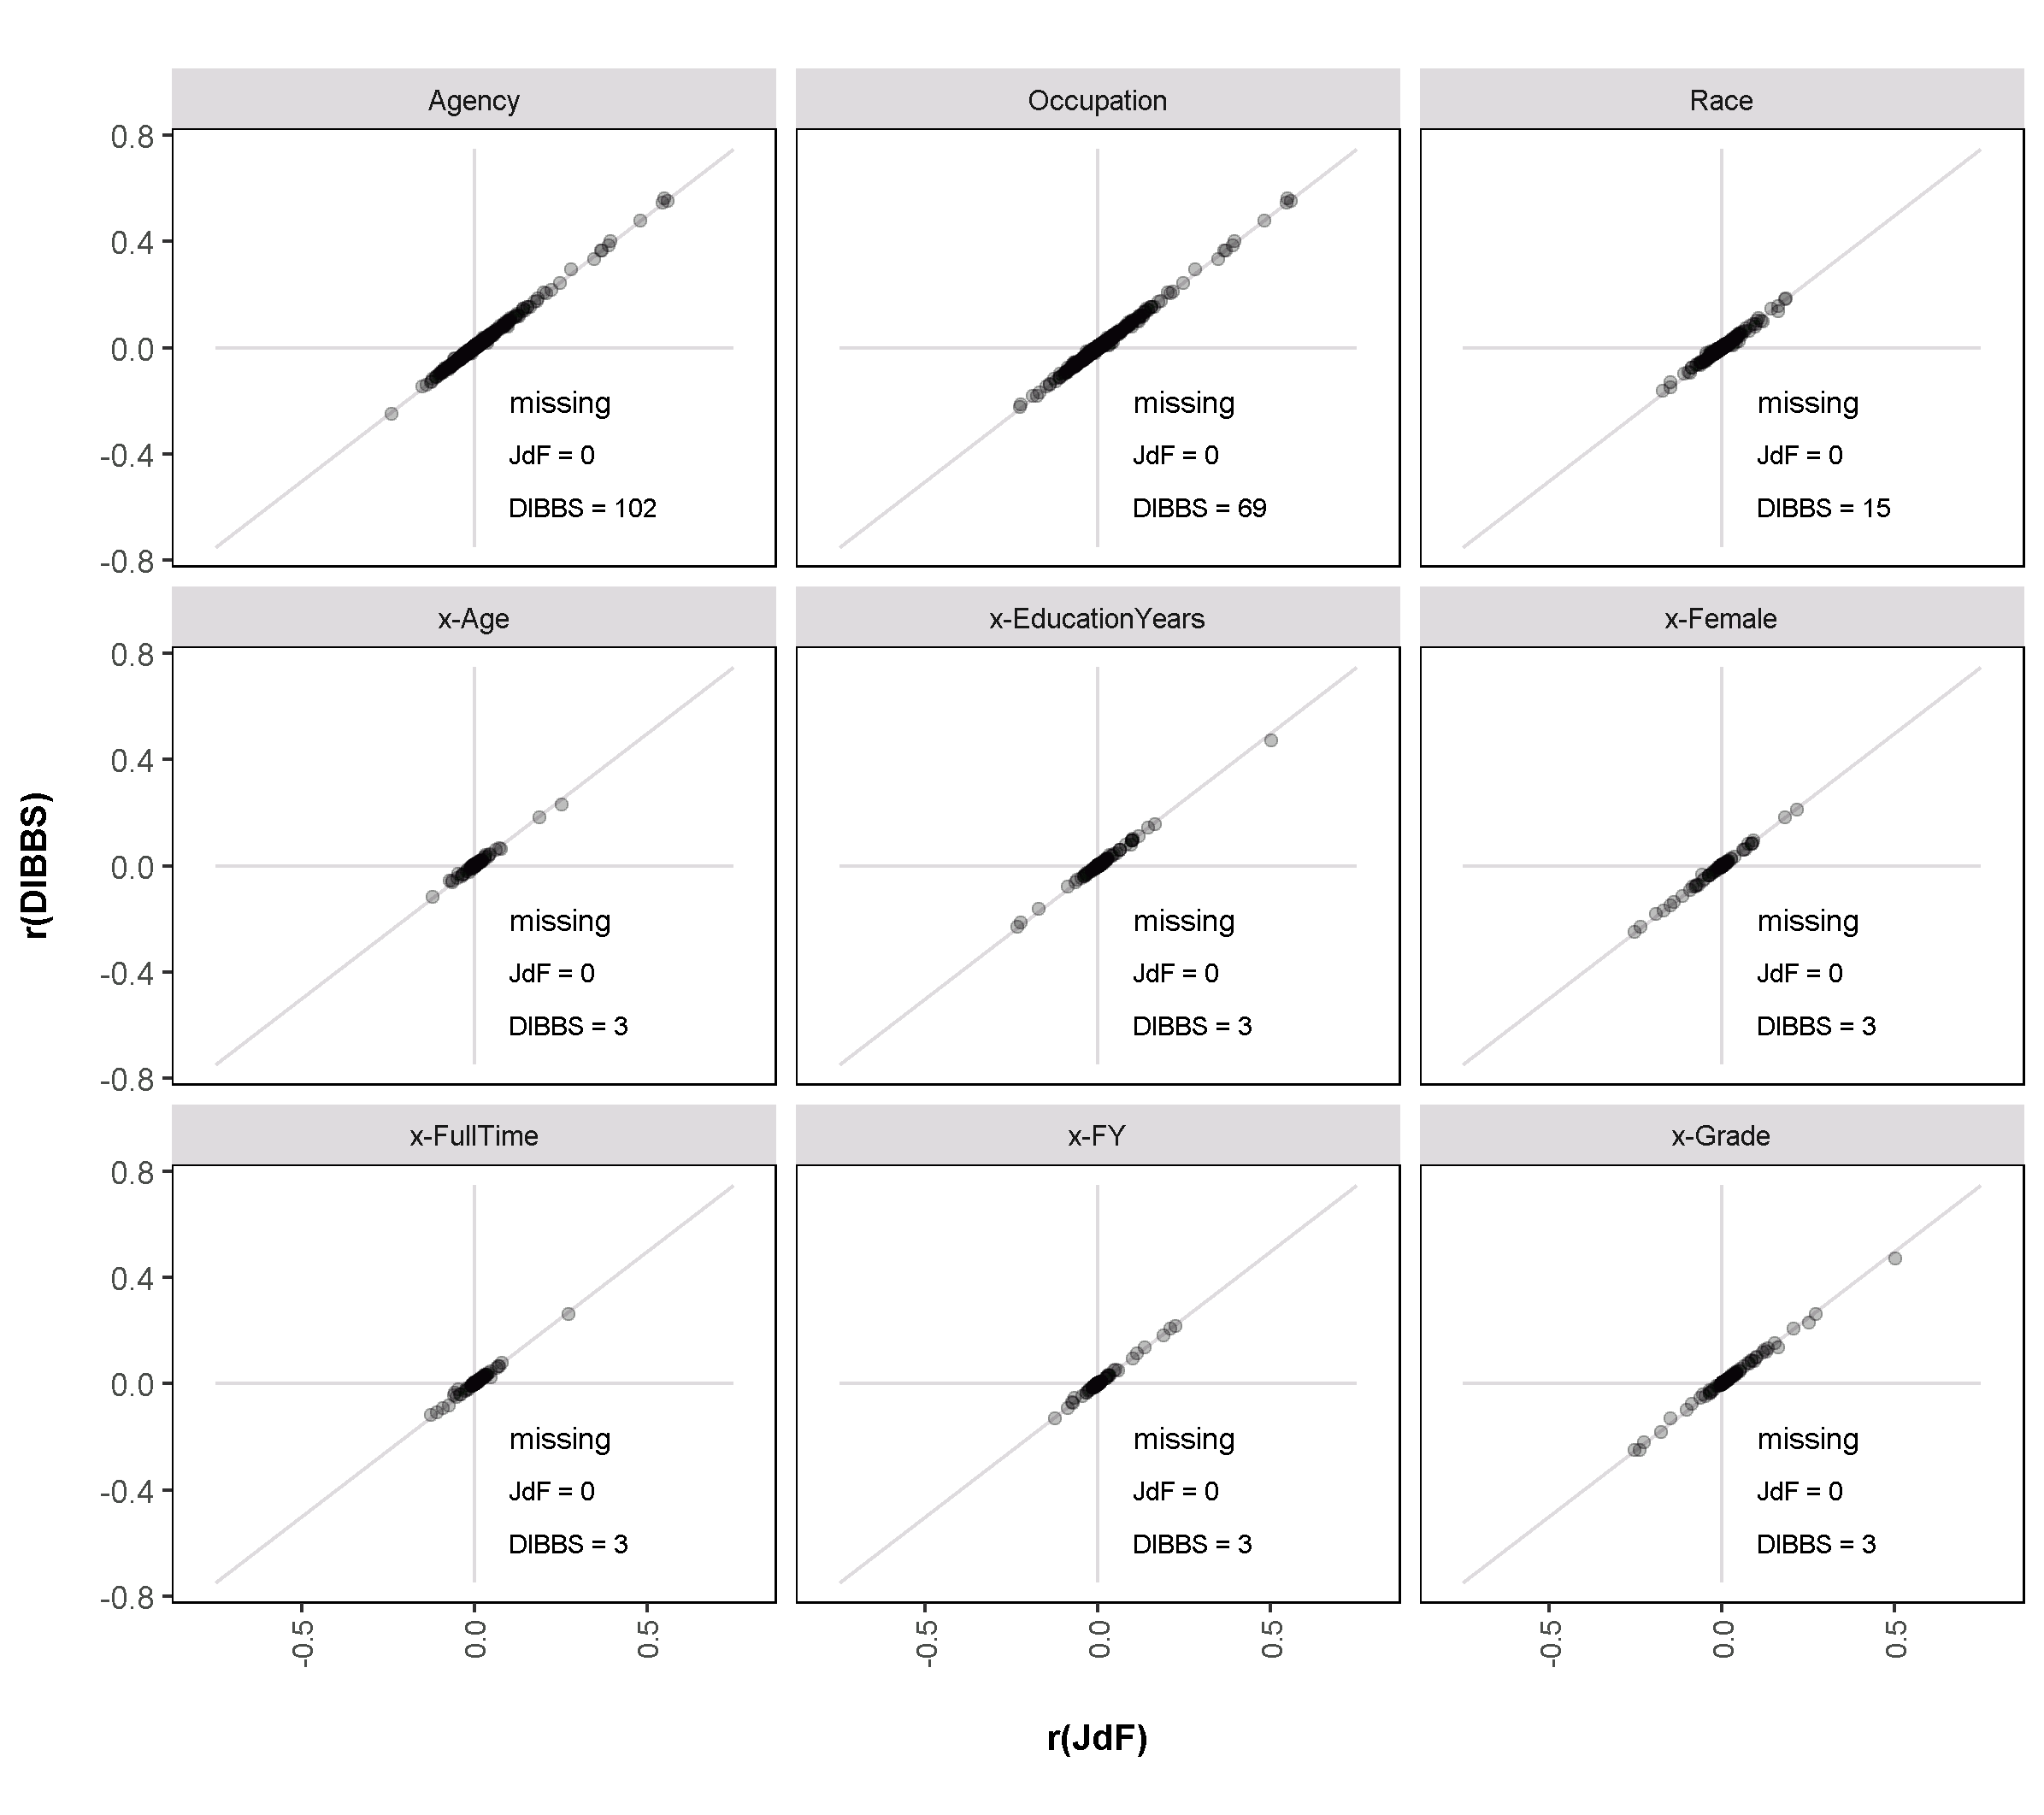
\includegraphics[width=5in]{JdFDIBBSCorrelation.png}
    \centering
    \caption{Two variable correlations of corresponding levels of synthetic and authentic data.  Synthetic level correlation on y-axis, corresponding authentic correlation on x-axis.}
    \label{figure:JdFDIBBSCorrelation}
\end{figure}  

\clearpage

\subsection{Correlation of Primary Variables With Two-Variable Interactions}

Figures \ref{figure:JdFDIBBSCorrelationInteraction1} through \ref{figure:JdFDIBBSCorrelationInteraction5} show correlations between 1.) the variable indicated in the graph title, 2.) all combinations of levels of the variable listed in a title bar, and 3.) all levels of other variables appearing in the title bars.  These constitute correlation of main variables with two variable interactions.  In the case of categorical variables, or fixed effects, this is the association of a primary variable with the proportion of observations in interacting level combinations of two other variables.  Agency and occupation truncated to first two positions.\\

Observation:  Proximity of all points to the slope 1.0 reference line indicates agreement of three-variable associations between data sets and implies depth of utility beyond simple pairwise relationships.\\

\vspace{20pt}

\begin{figure}[h]
    \centering
    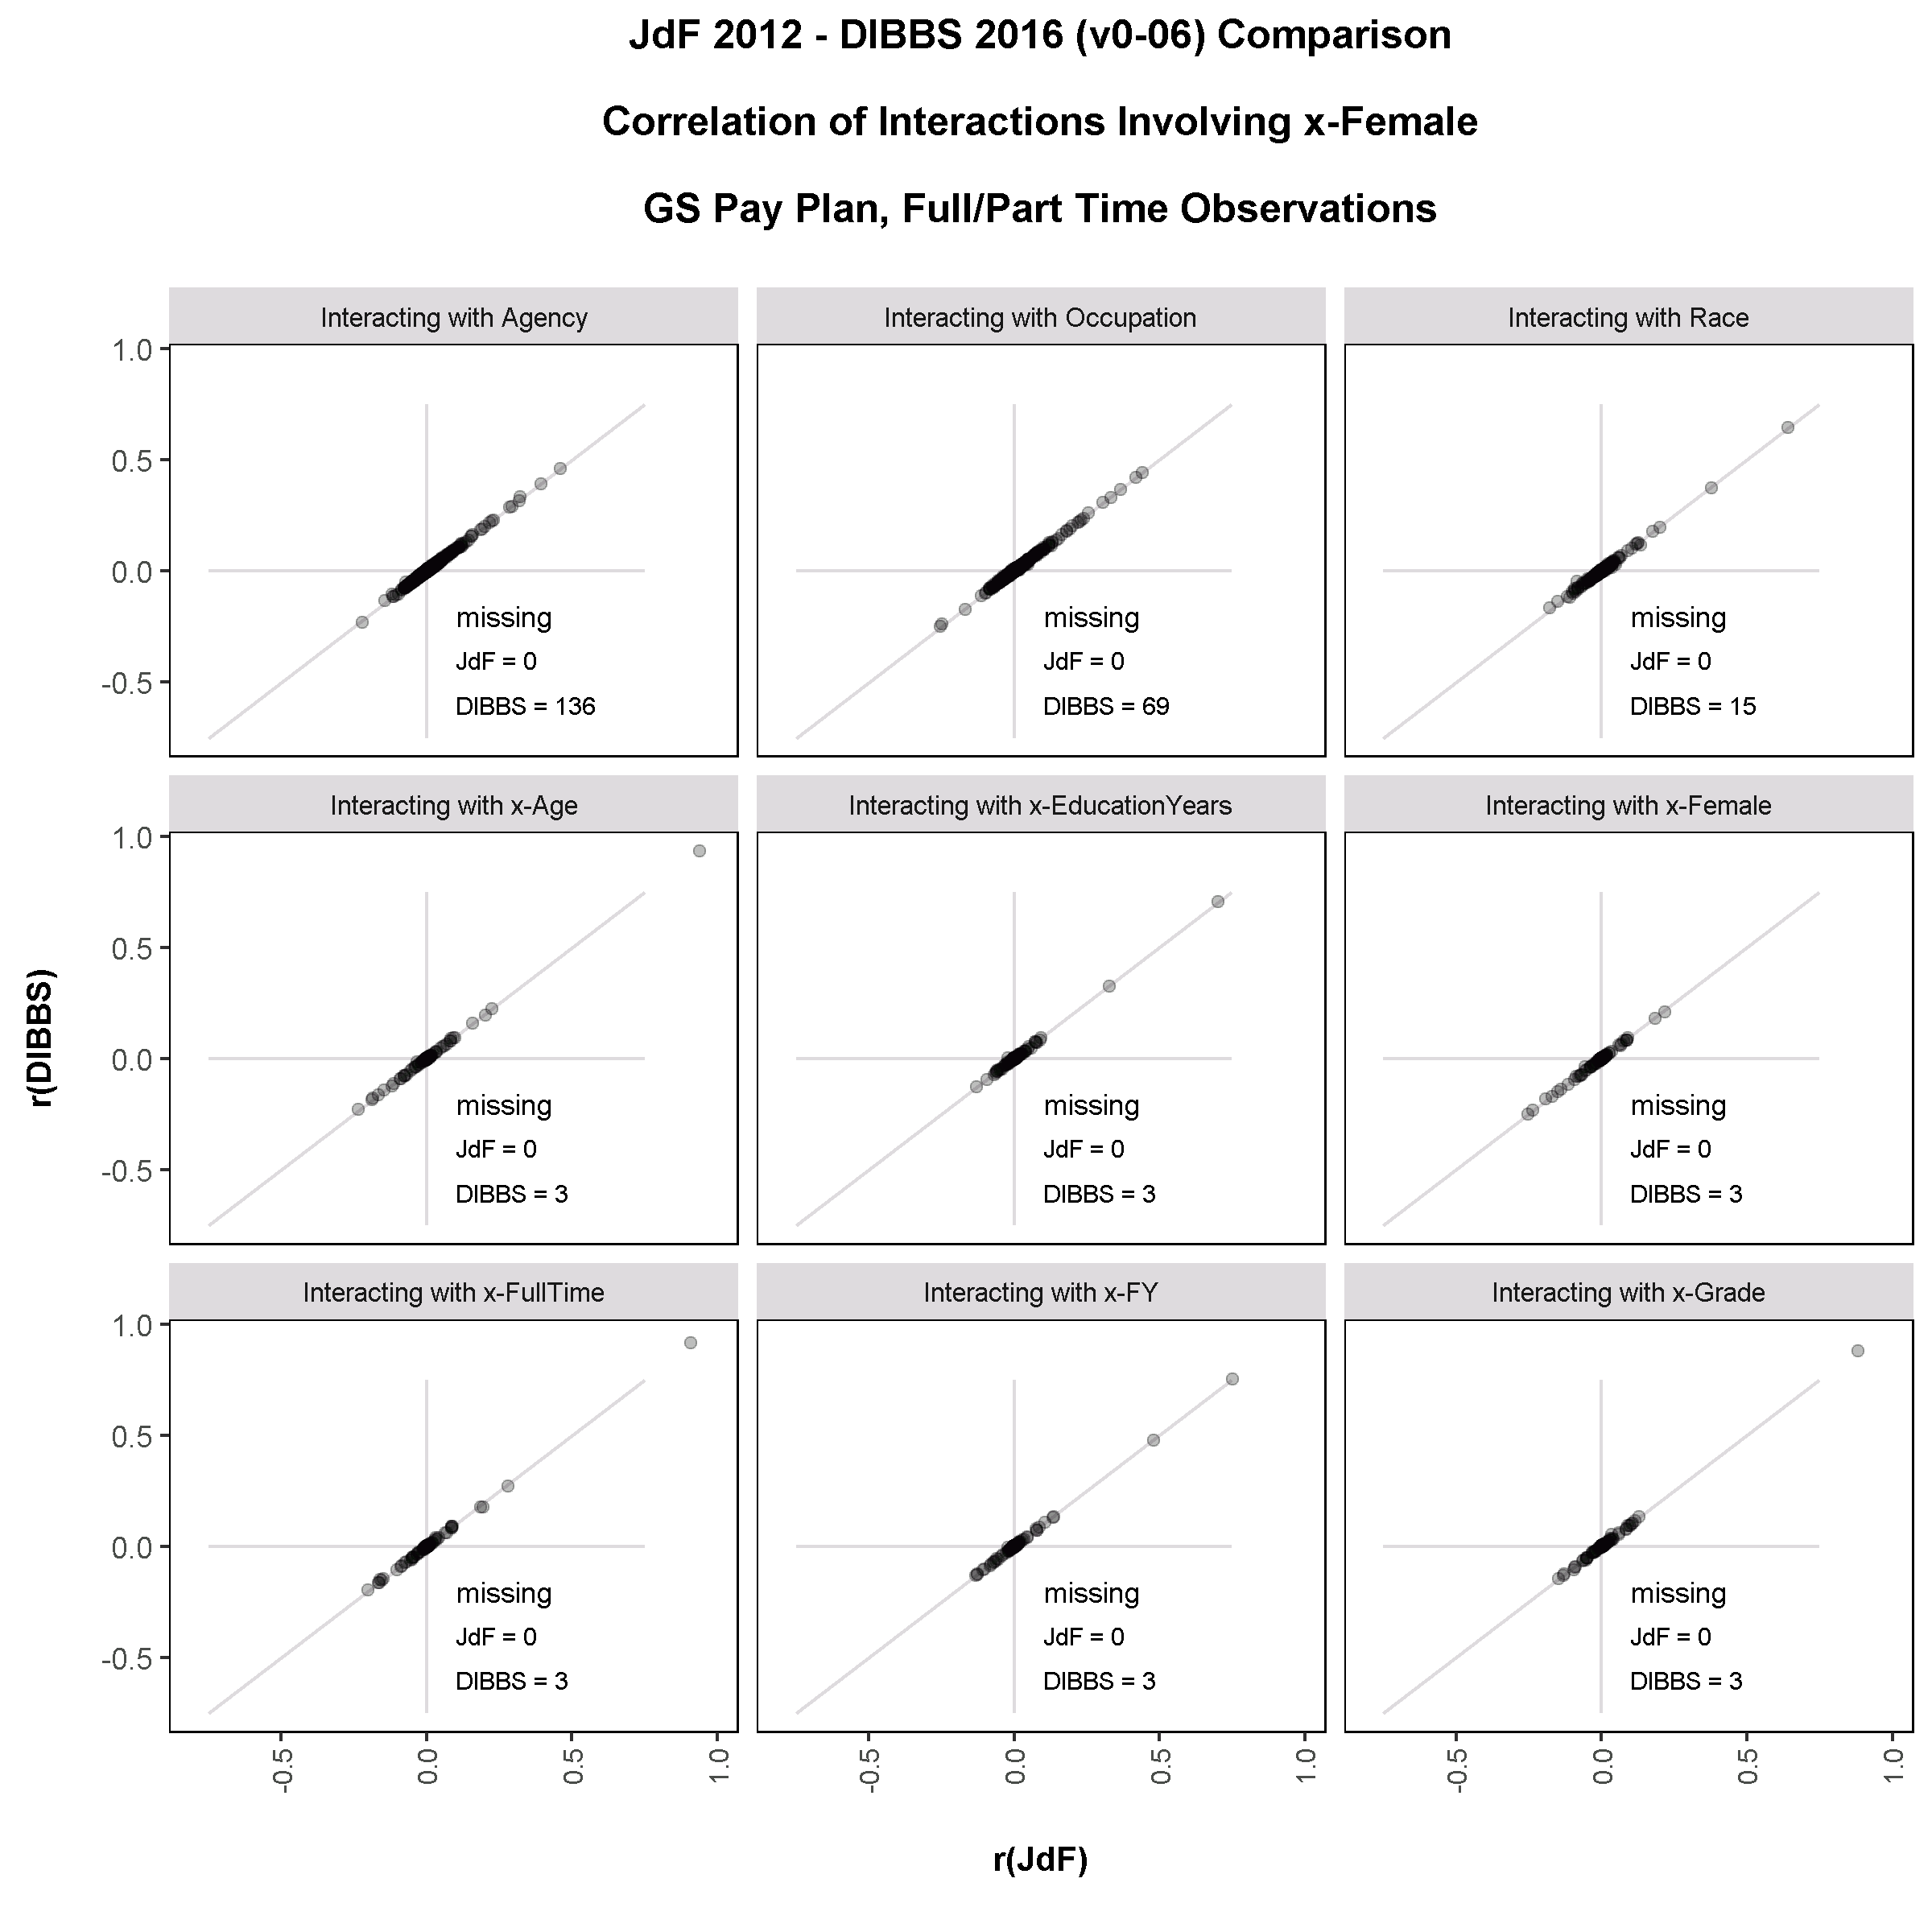
\includegraphics[width=5in, trim={0 0.2in 0 1in}, clip]{JdFDIBBSCorrelationInteraction-x-Female.png}
    \caption{Correlation of primary variables with two variable interactions.  Variable set one, involving sex.  Synthetic level correlation on y-axis, corresponding authentic correlation on x-axis.}
    \label{figure:JdFDIBBSCorrelationInteraction1}
\end{figure}

\clearpage

\begin{figure}[h]
    \centering
    \begin{subfigure}{1\textwidth}
        \centering
        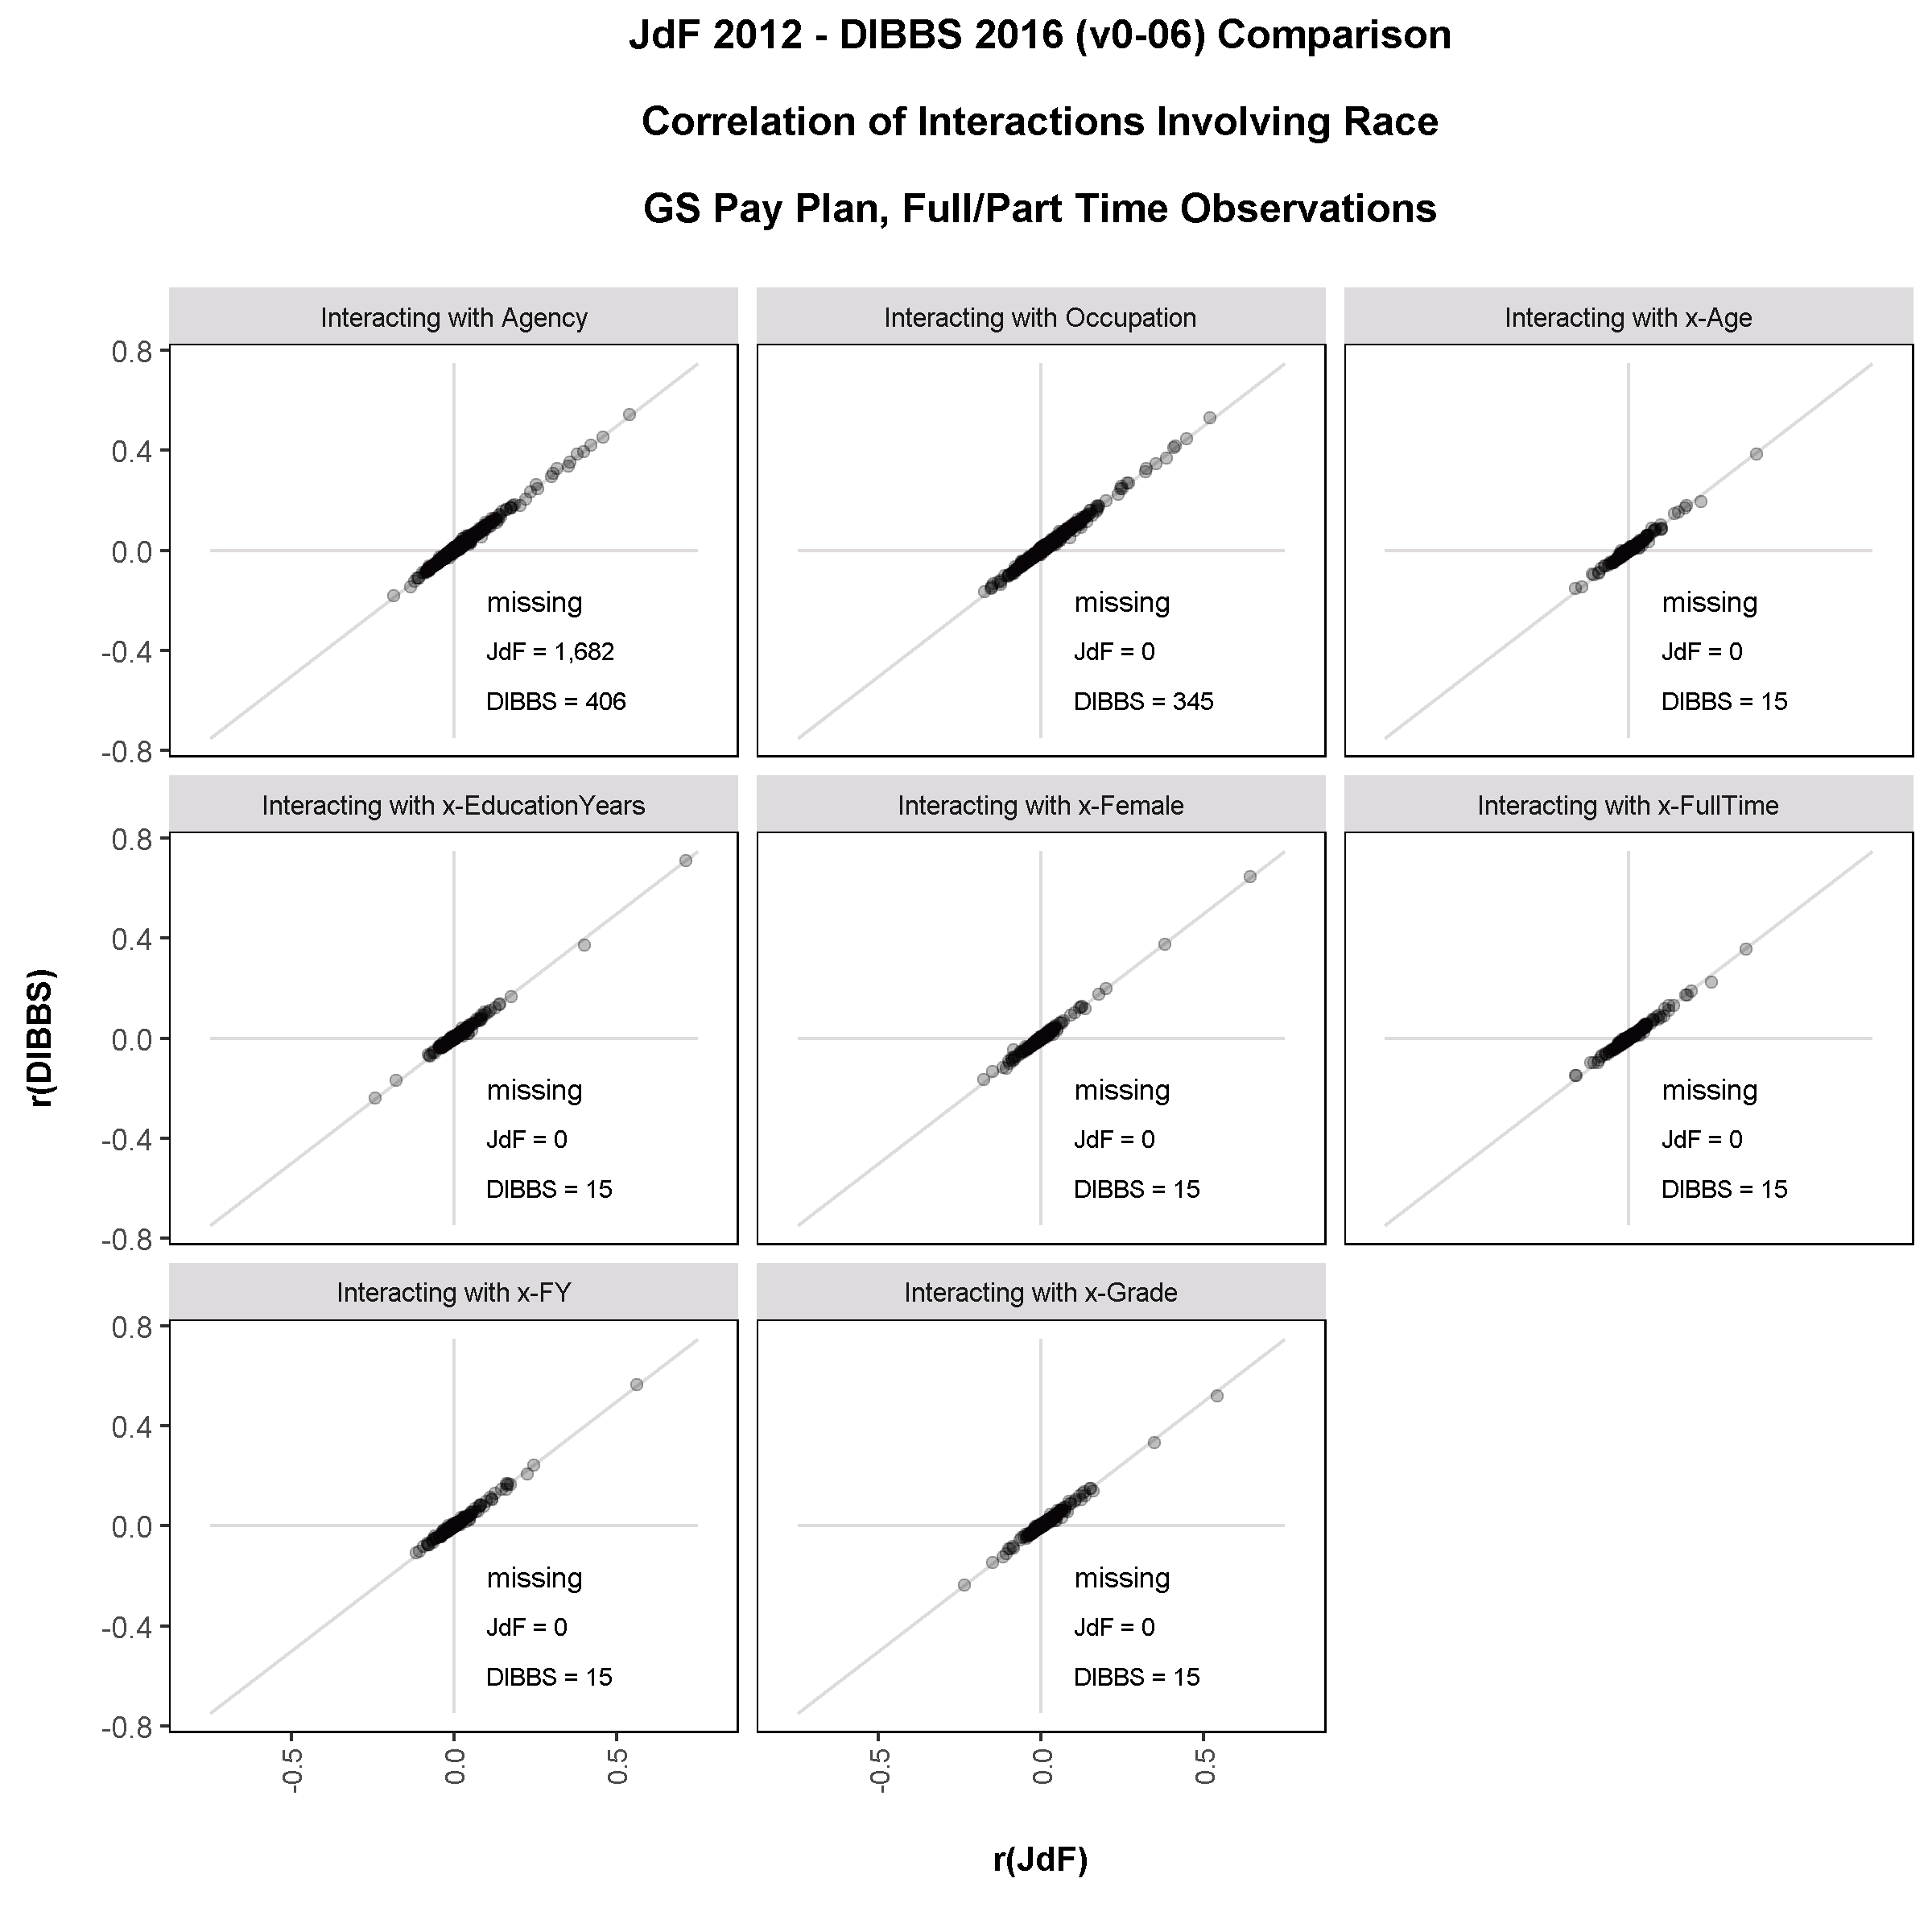
\includegraphics[width=4.5in, trim={0 0.2in 0 1in}, clip]{JdFDIBBSCorrelationInteraction-Race.png}
        \caption{Correlations involving race}
        \vspace{12pt}
    \end{subfigure}
    \begin{subfigure}{1\textwidth}
        \centering
        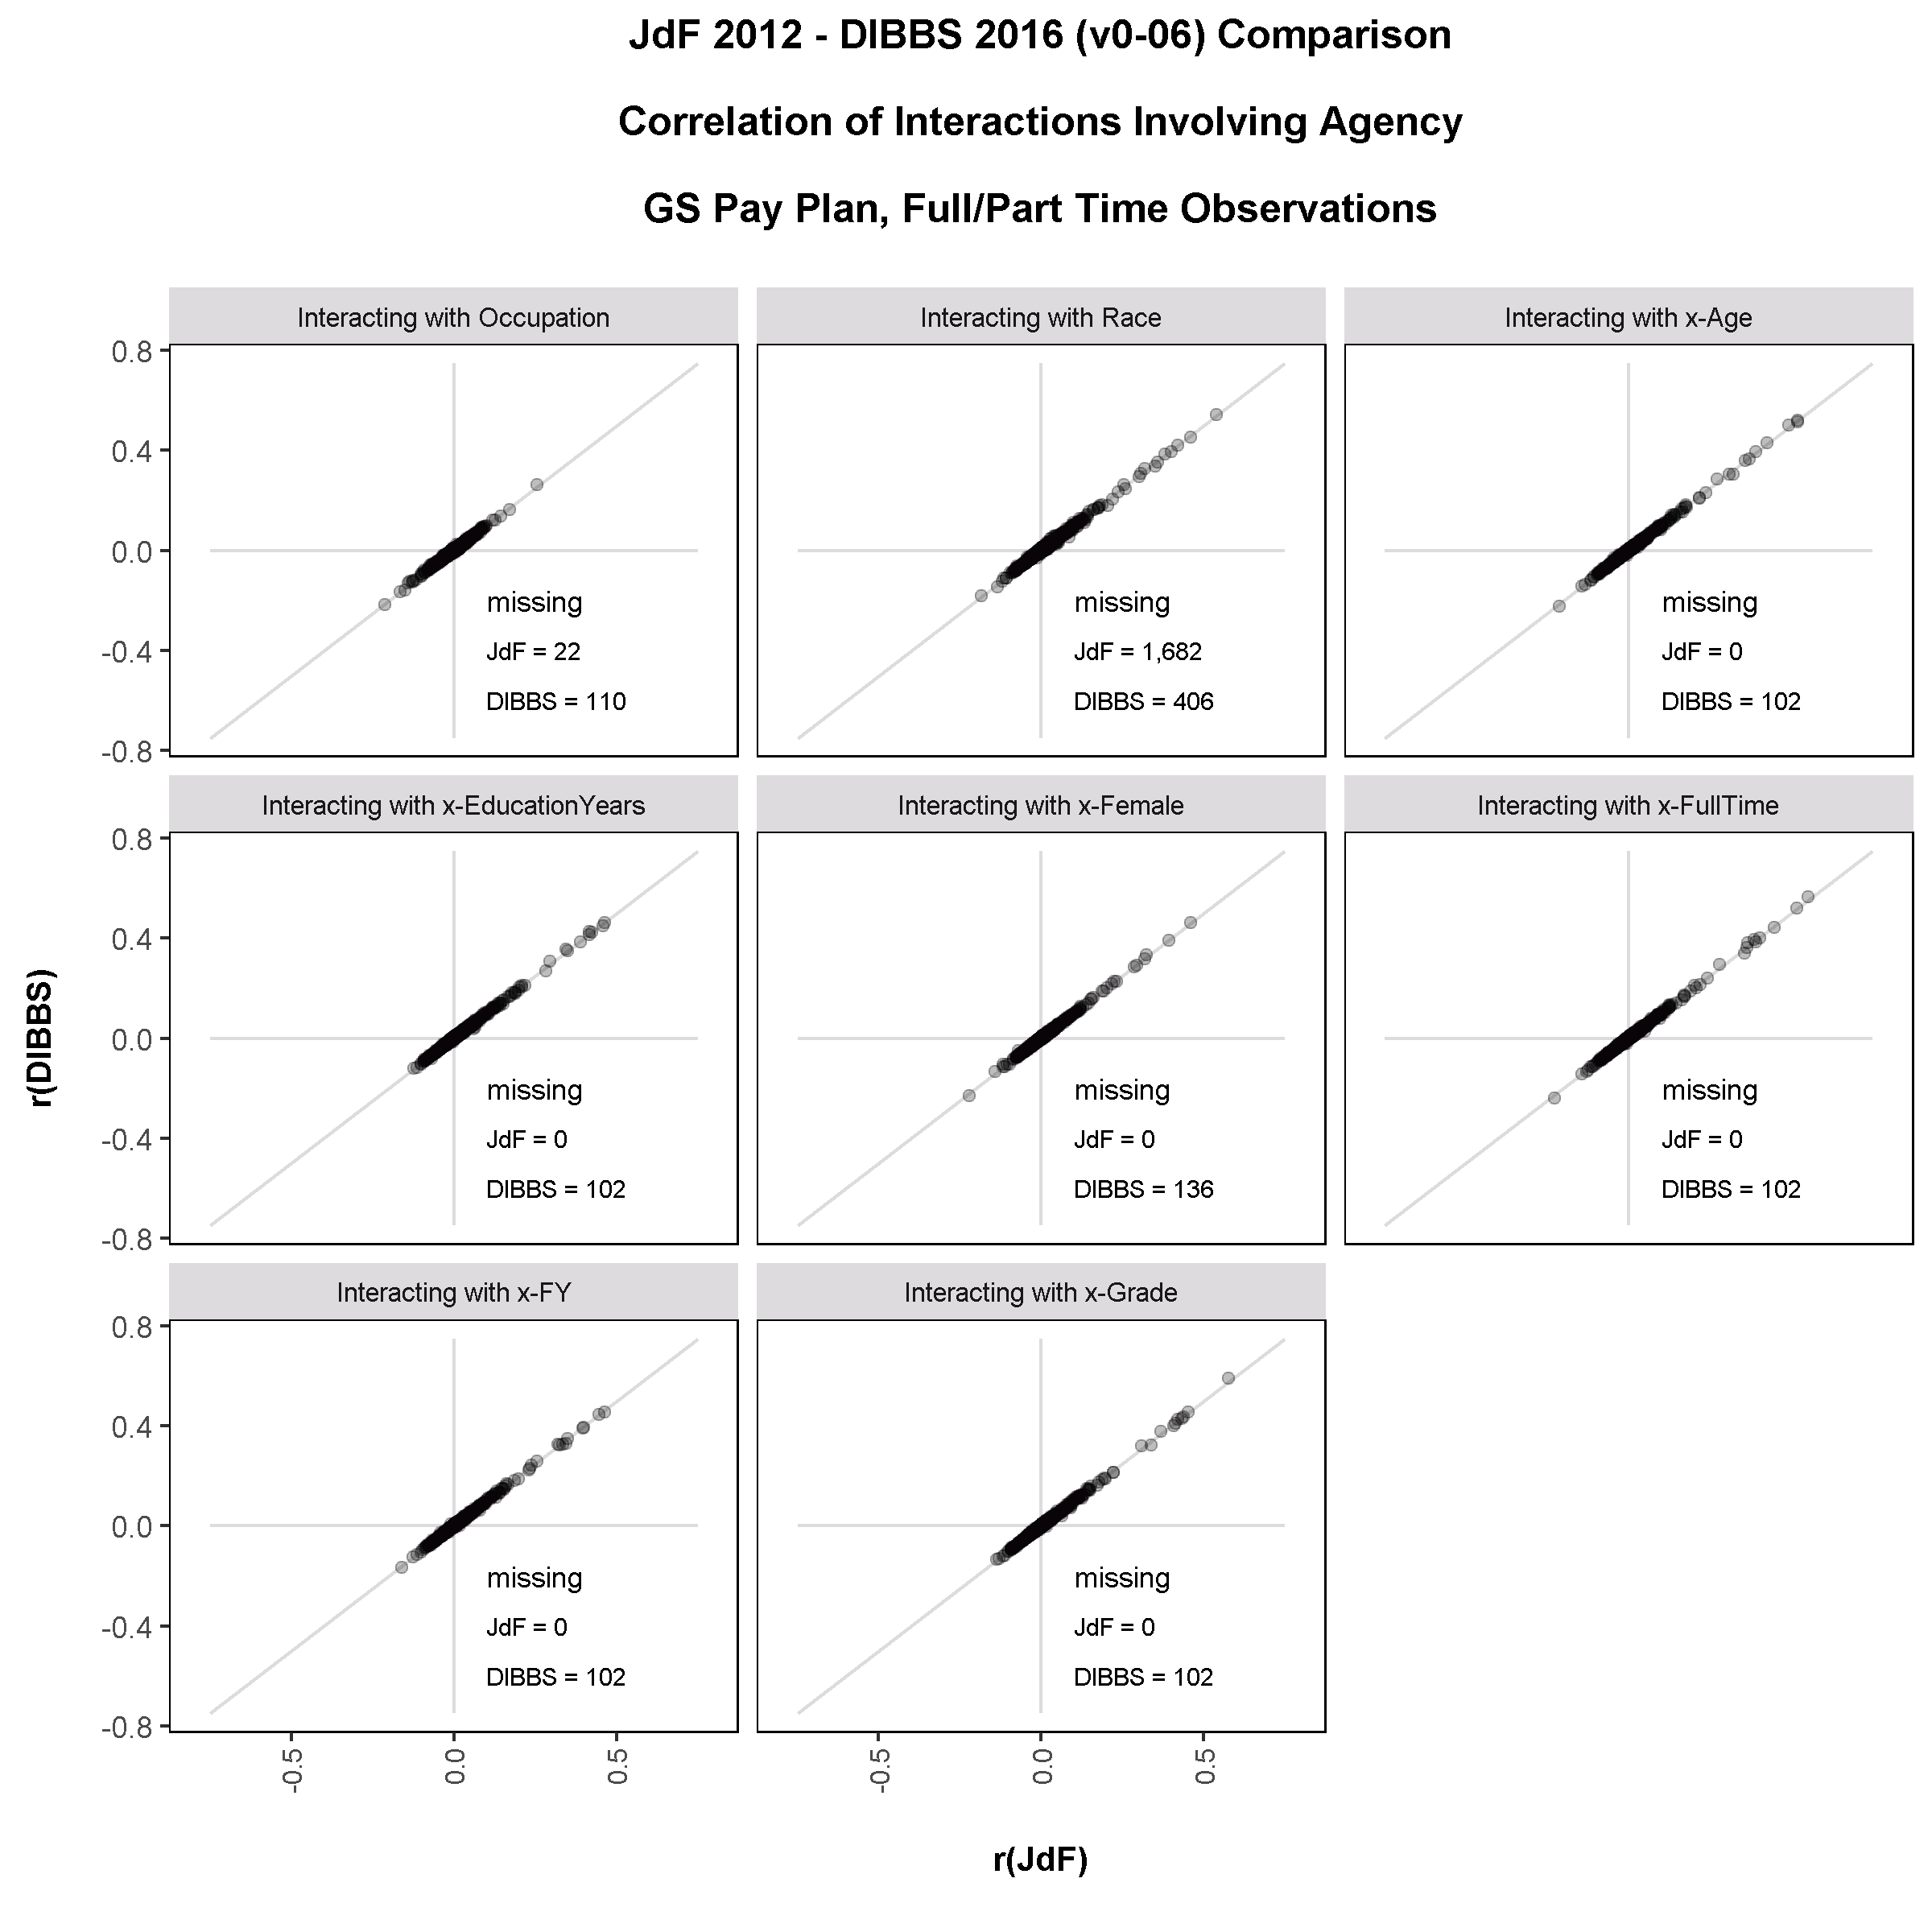
\includegraphics[width=4.5in, trim={0 0.2in 0 1in}, clip]{JdFDIBBSCorrelationInteraction-Agency.png}
        \caption{Correlations involving agency}
        \vspace{12pt}
    \end{subfigure}
    \caption{Correlation of primary variables with two variable interactions.  Variable set two.  Synthetic level correlation on y-axis, corresponding authentic correlation on x-axis.}
    \label{figure:JdFDIBBSCorrelationInteraction2}
\end{figure}

\clearpage

\begin{figure}[h]
    \centering
    \begin{subfigure}{1\textwidth}
        \centering
        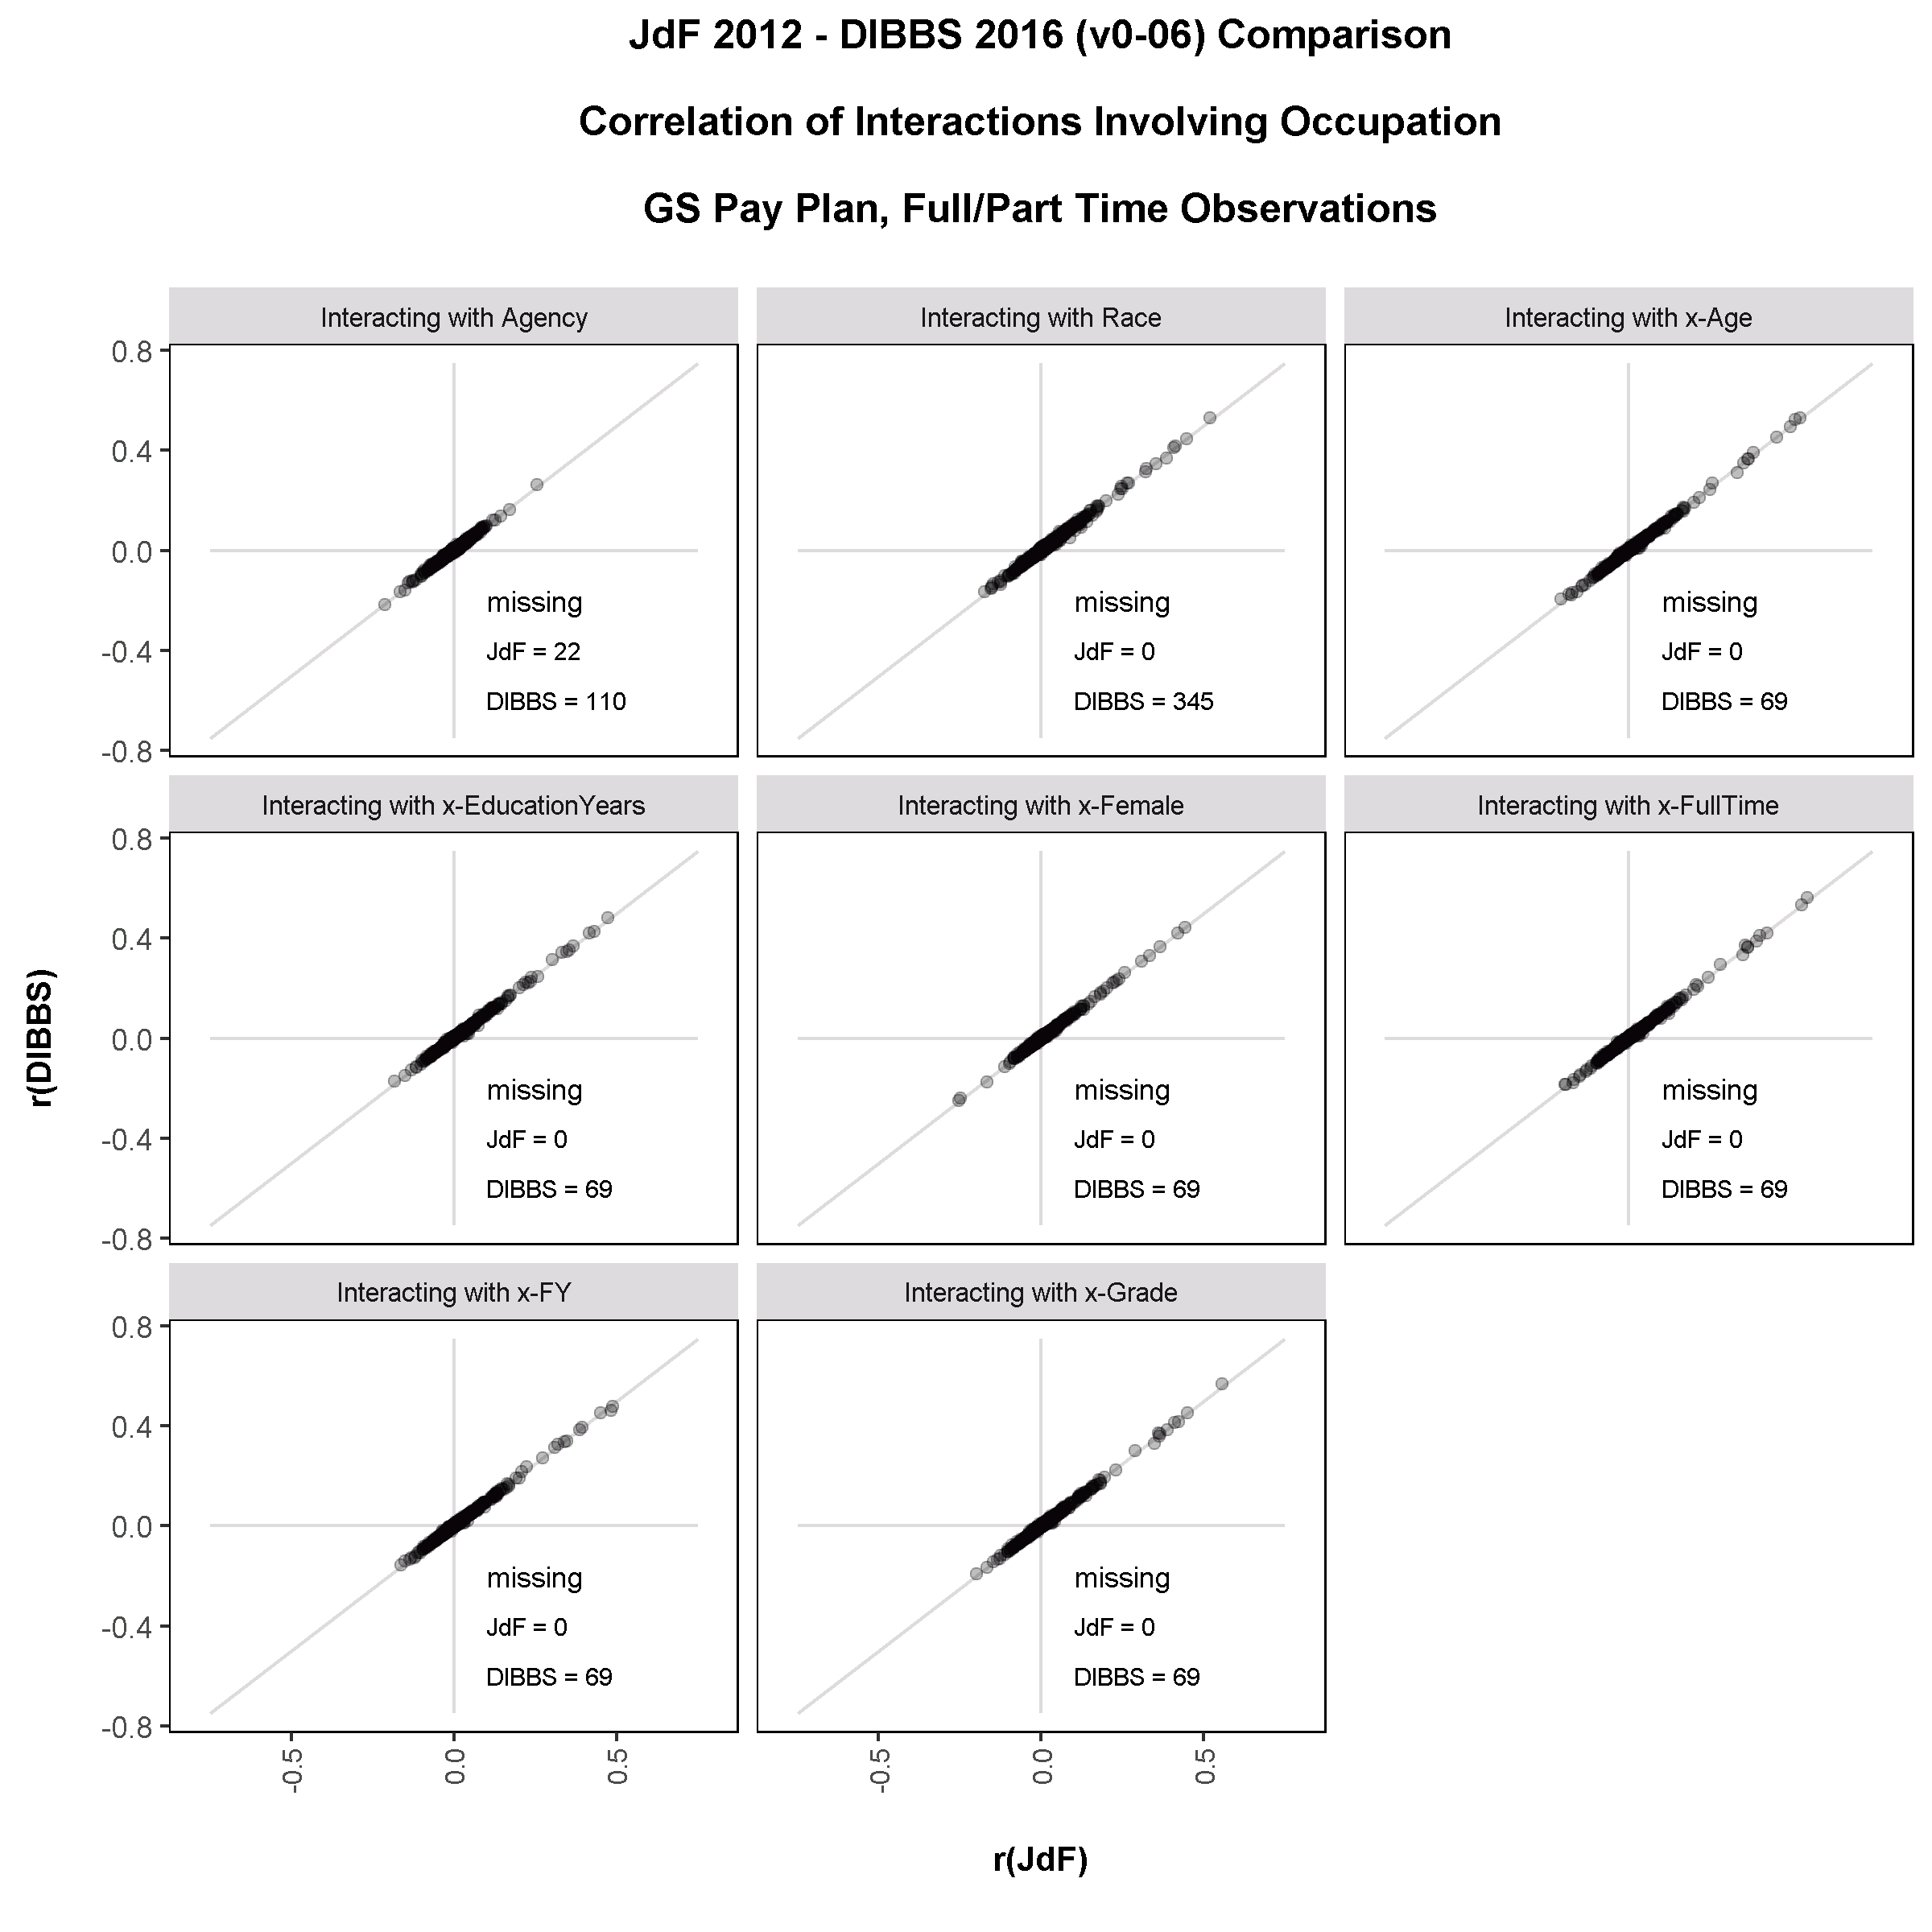
\includegraphics[width=4.5in, trim={0 0.2in 0 1in}, clip]{JdFDIBBSCorrelationInteraction-Occupation.png}
        \caption{Correlations involving occupation}
        \vspace{12pt}
    \end{subfigure}
    \begin{subfigure}{1\textwidth}
        \centering
        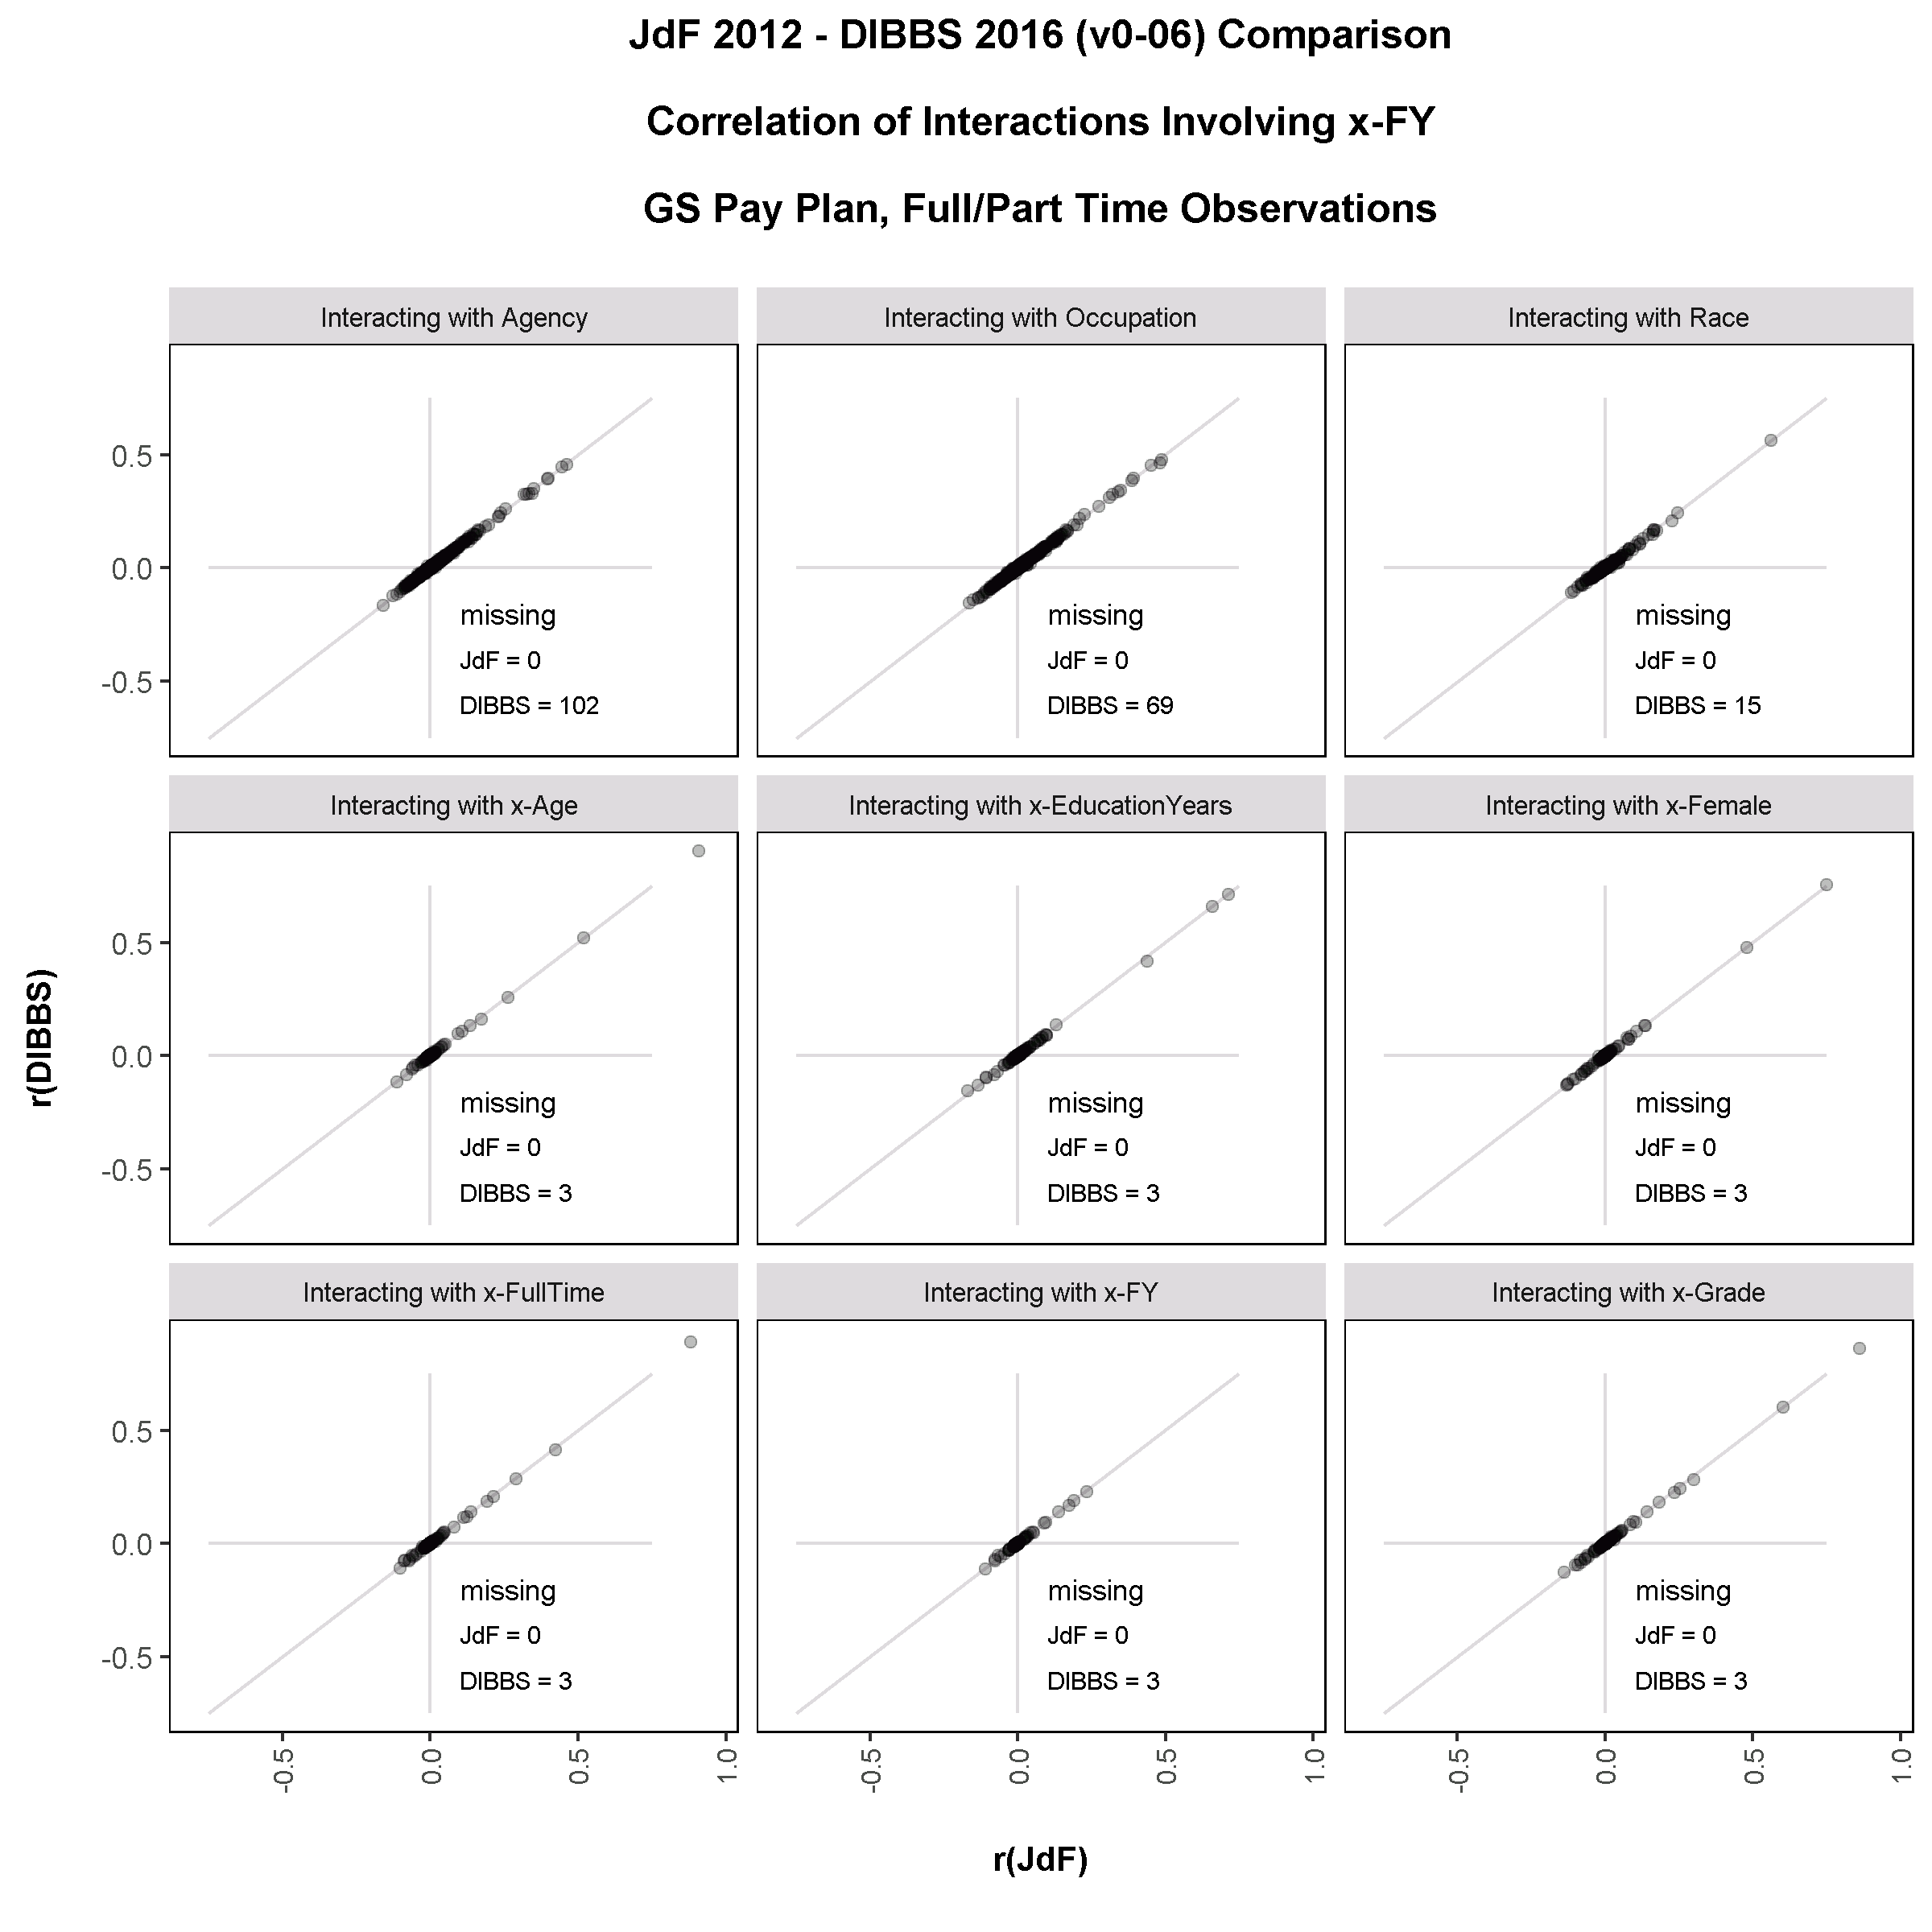
\includegraphics[width=4.5in, trim={0 0.2in 0 1in}, clip]{JdFDIBBSCorrelationInteraction-x-FY.png}
        \caption{Correlations involving fiscal year}
        \vspace{12pt}
    \end{subfigure}
    \caption{Correlation of primary variables with two variable interactions.  Variable set three.  Synthetic level correlation on y-axis, corresponding authentic correlation on x-axis.}
    \label{figure:JdFDIBBSCorrelationInteraction3}
\end{figure}

\clearpage

\begin{figure}[h]
    \centering
    \begin{subfigure}{1\textwidth}
        \centering
        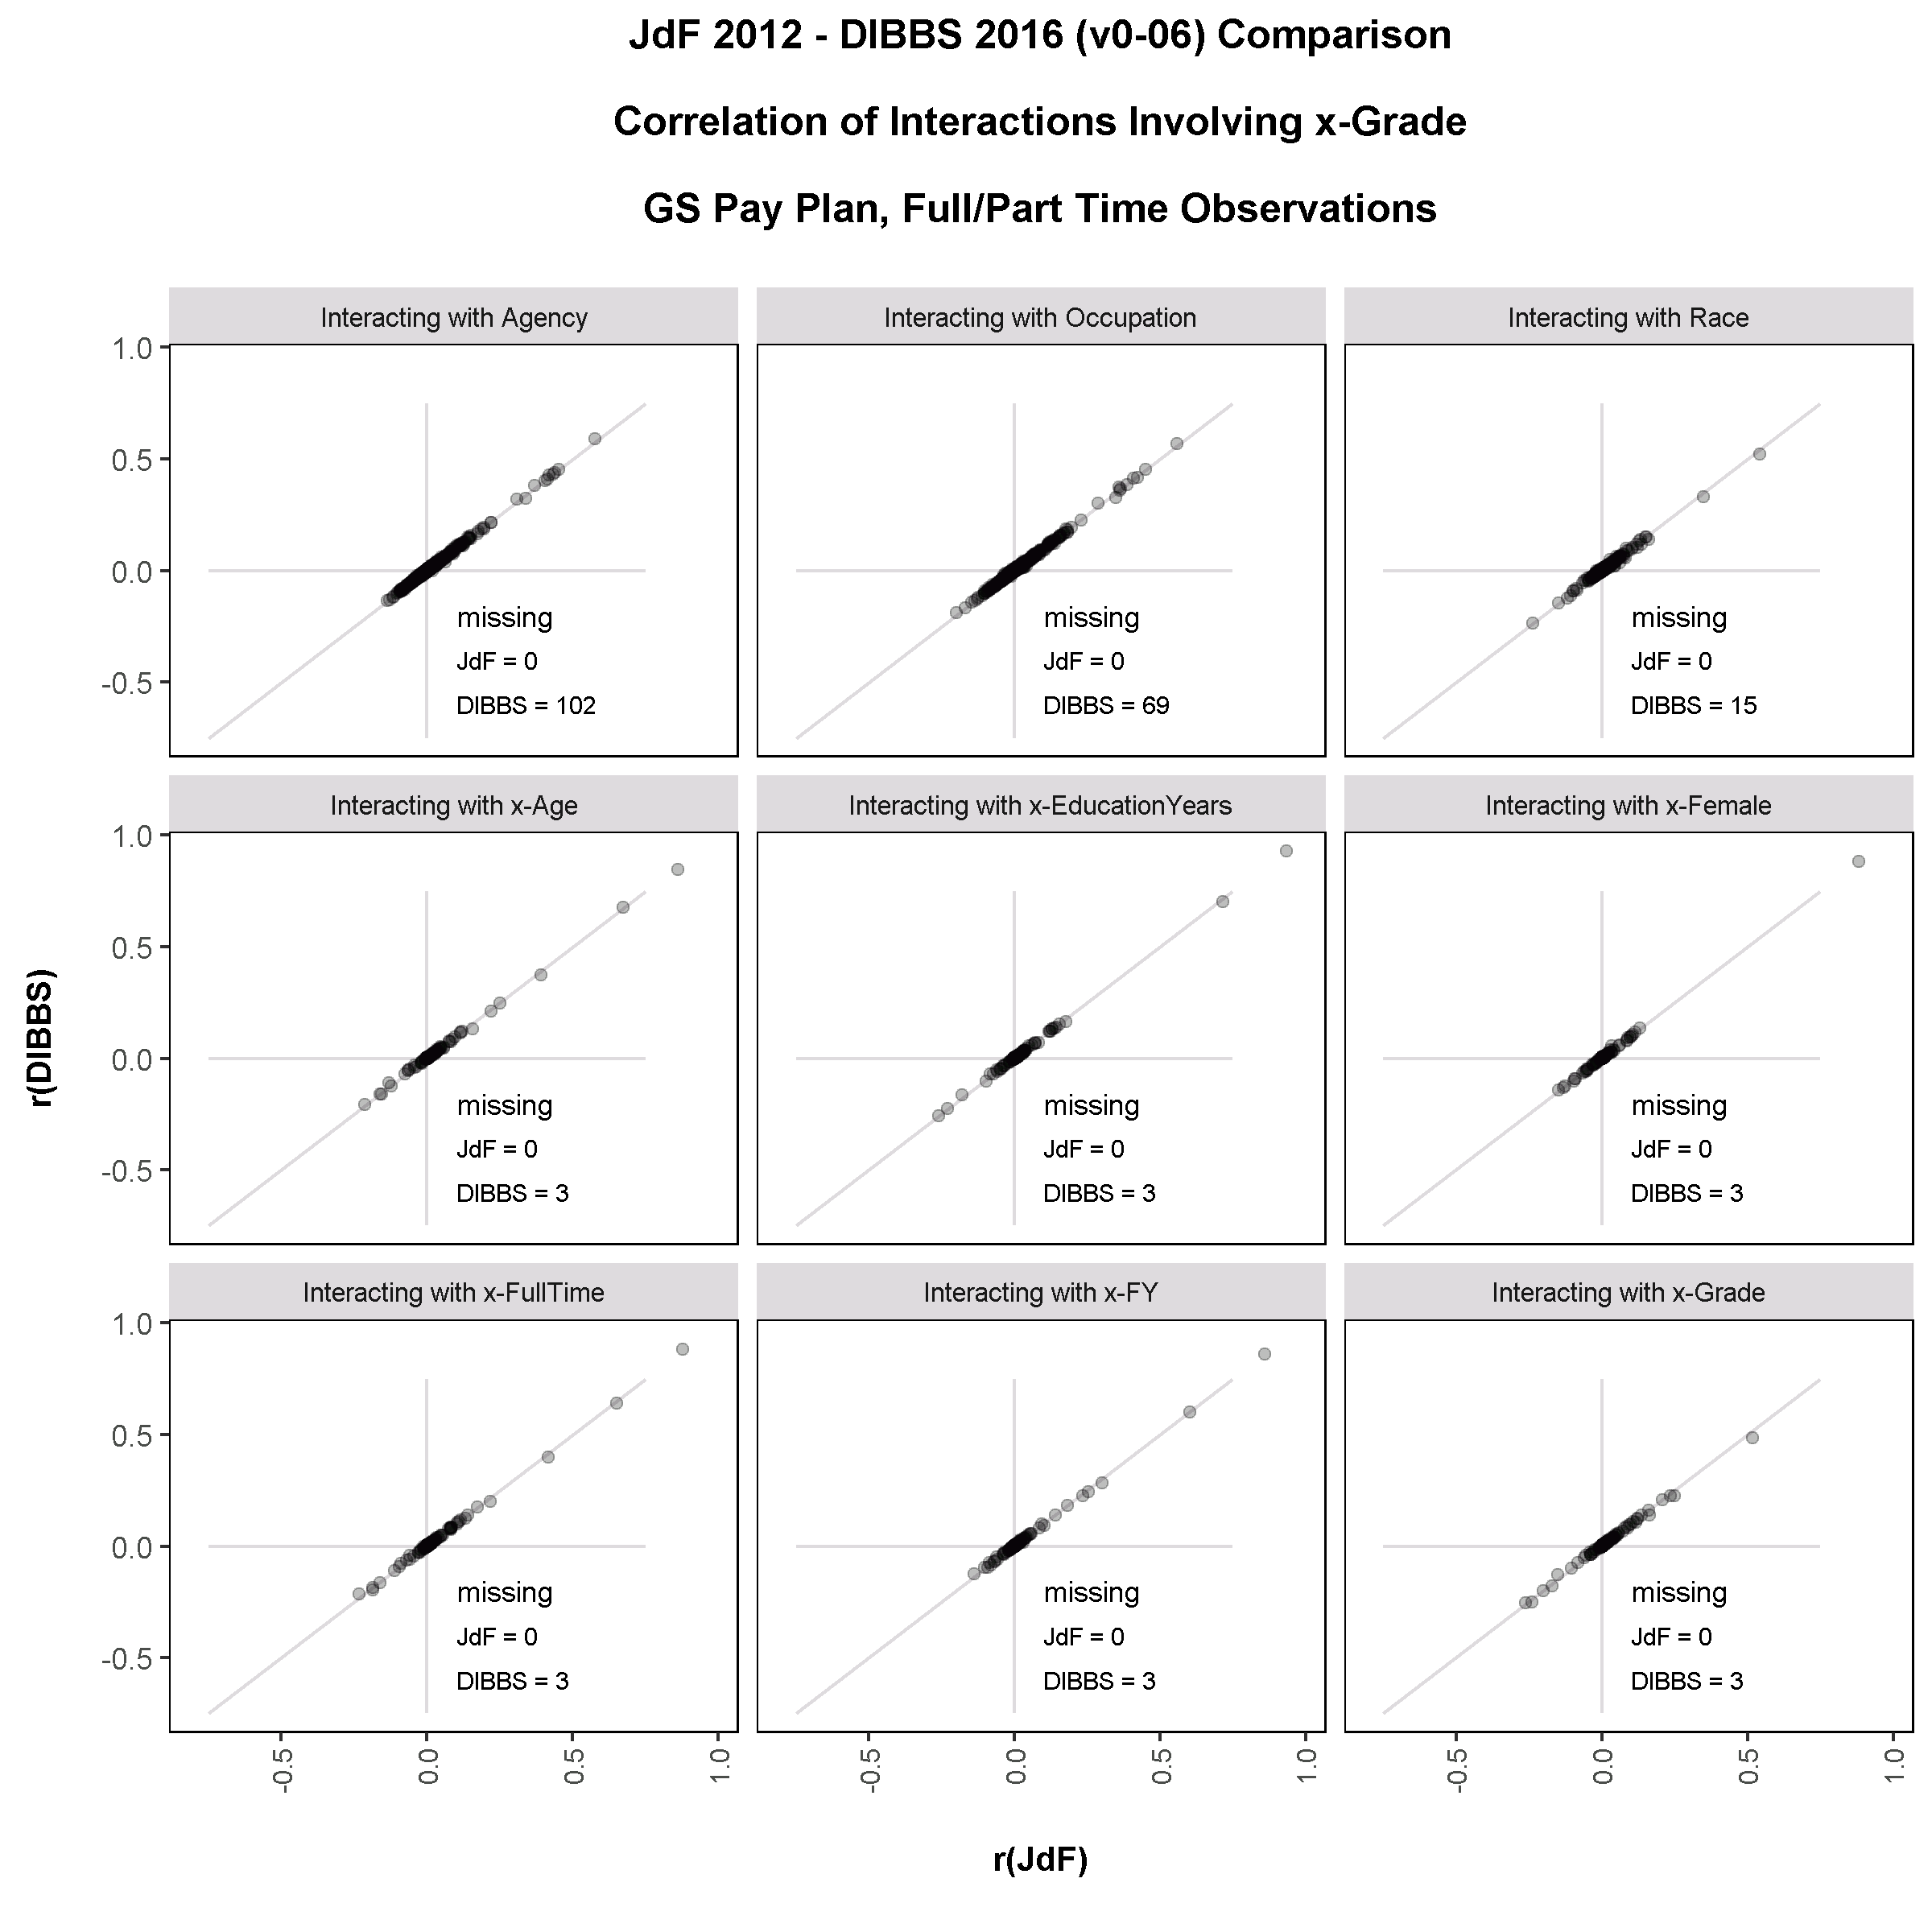
\includegraphics[width=4.5in, trim={0 0.2in 0 1in}, clip]{JdFDIBBSCorrelationInteraction-x-Grade.png}
        \caption{Correlations involving grade}
        \vspace{12pt}
    \end{subfigure}
    \begin{subfigure}{1\textwidth}
        \centering
        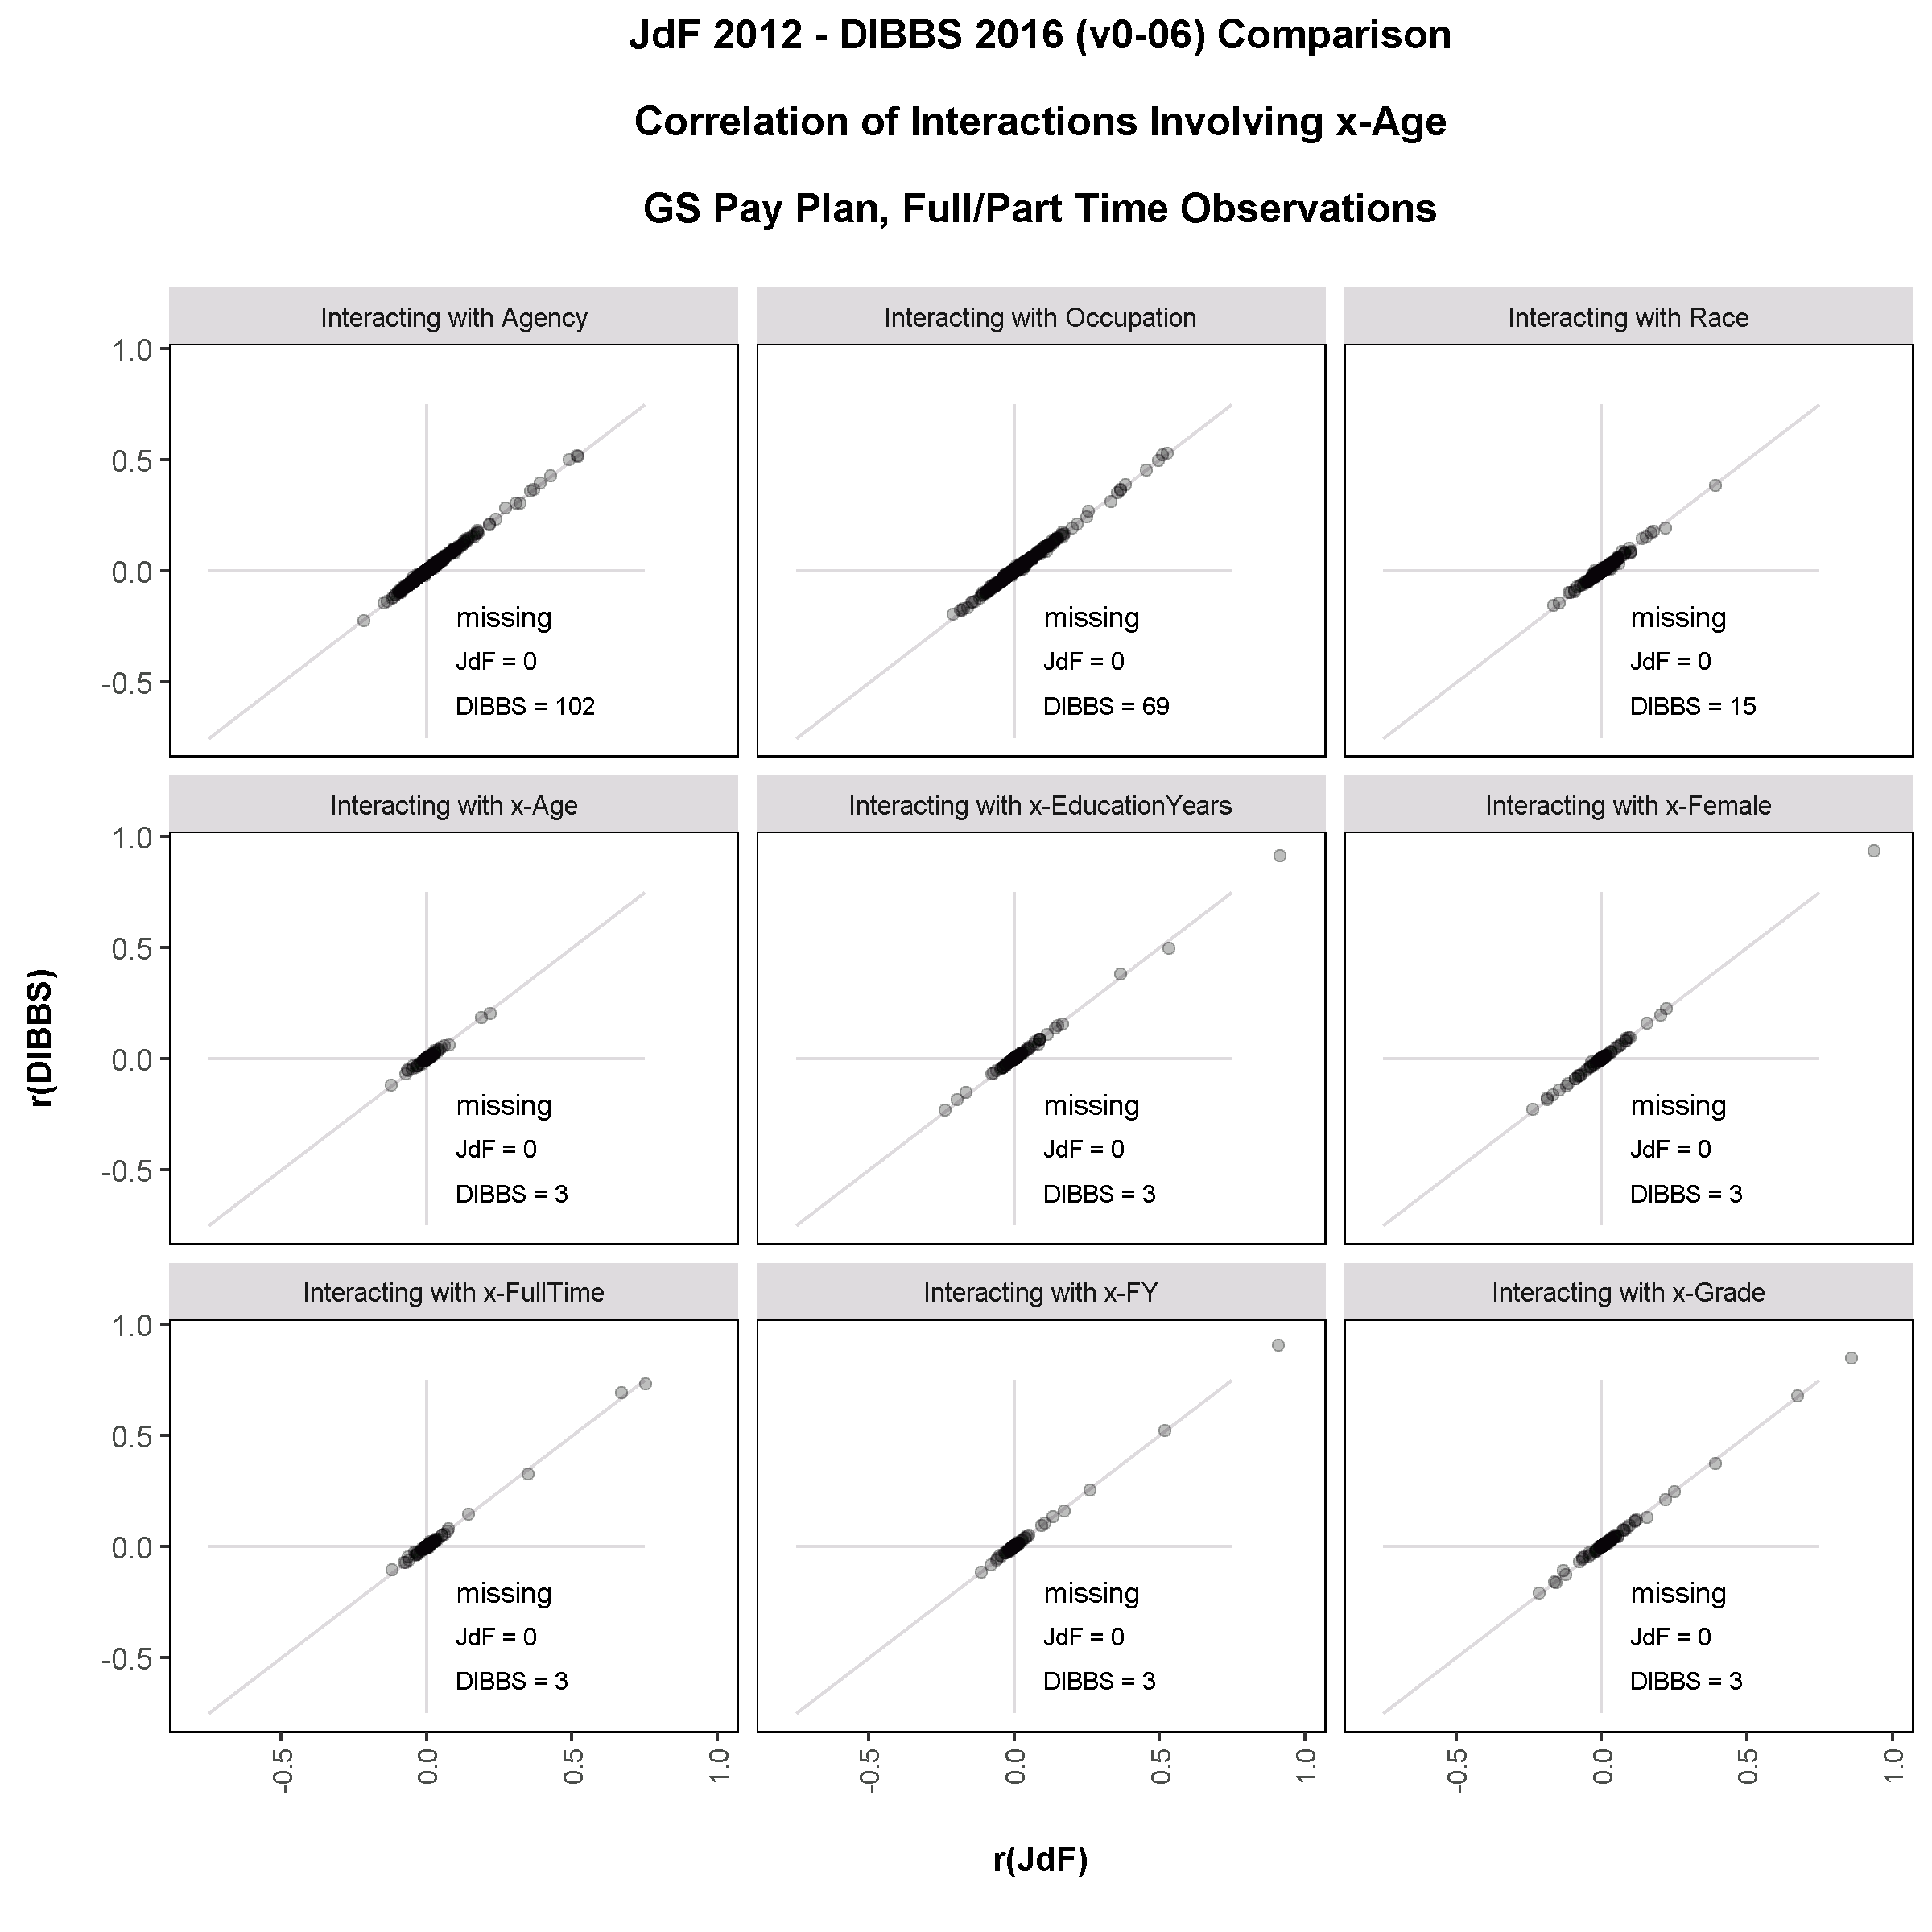
\includegraphics[width=4.5in, trim={0 0.2in 0 1in}, clip]{JdFDIBBSCorrelationInteraction-x-Age.png}
        \caption{Correlations involving age}
        \vspace{12pt}
    \end{subfigure}
    \caption{Correlation of primary variables with two variable interactions.  Variable set four.  Synthetic level correlation on y-axis, corresponding authentic correlation on x-axis.}
    \label{figure:JdFDIBBSCorrelationInteraction4}
\end{figure}

\clearpage

\begin{figure}[h]
    \centering
    \begin{subfigure}{1\textwidth}
        \centering
        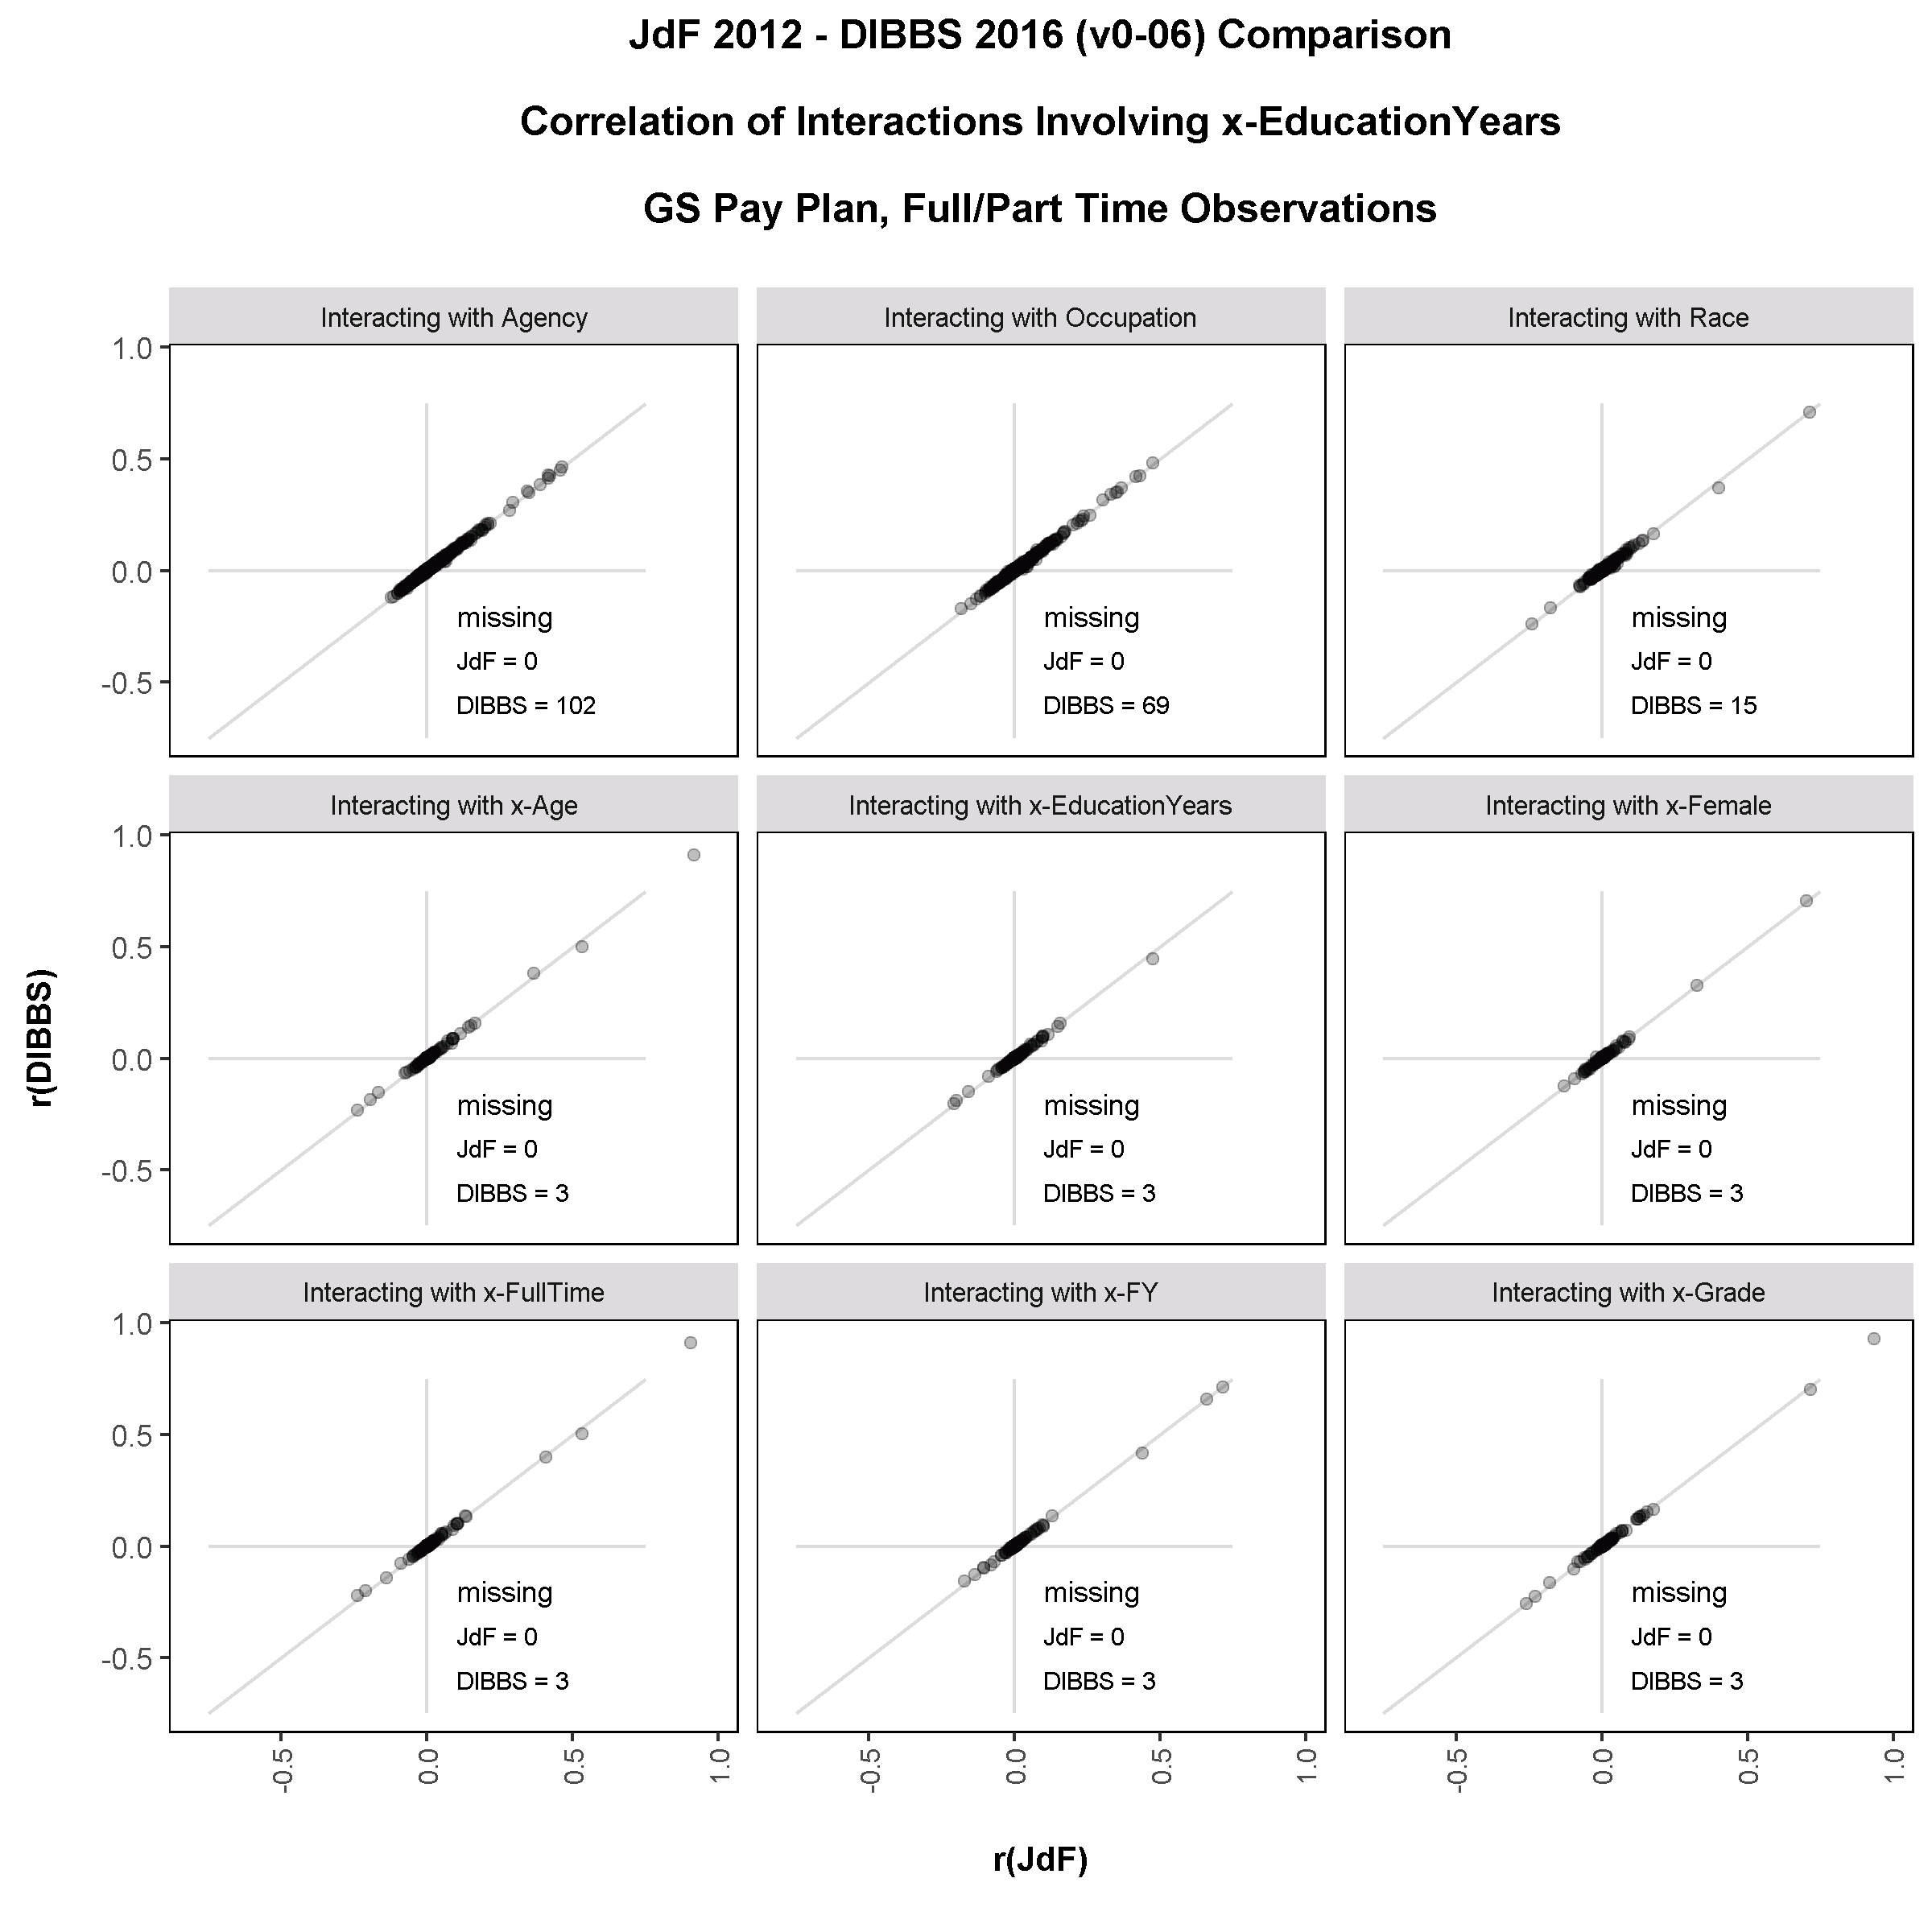
\includegraphics[width=4.5in, trim={0 0.2in 0 1in}, clip]{JdFDIBBSCorrelationInteraction-x-EducationYears.png}
        \caption{Correlations involving education}
        \vspace{12pt}
    \end{subfigure}
    \begin{subfigure}{1\textwidth}
        \centering
        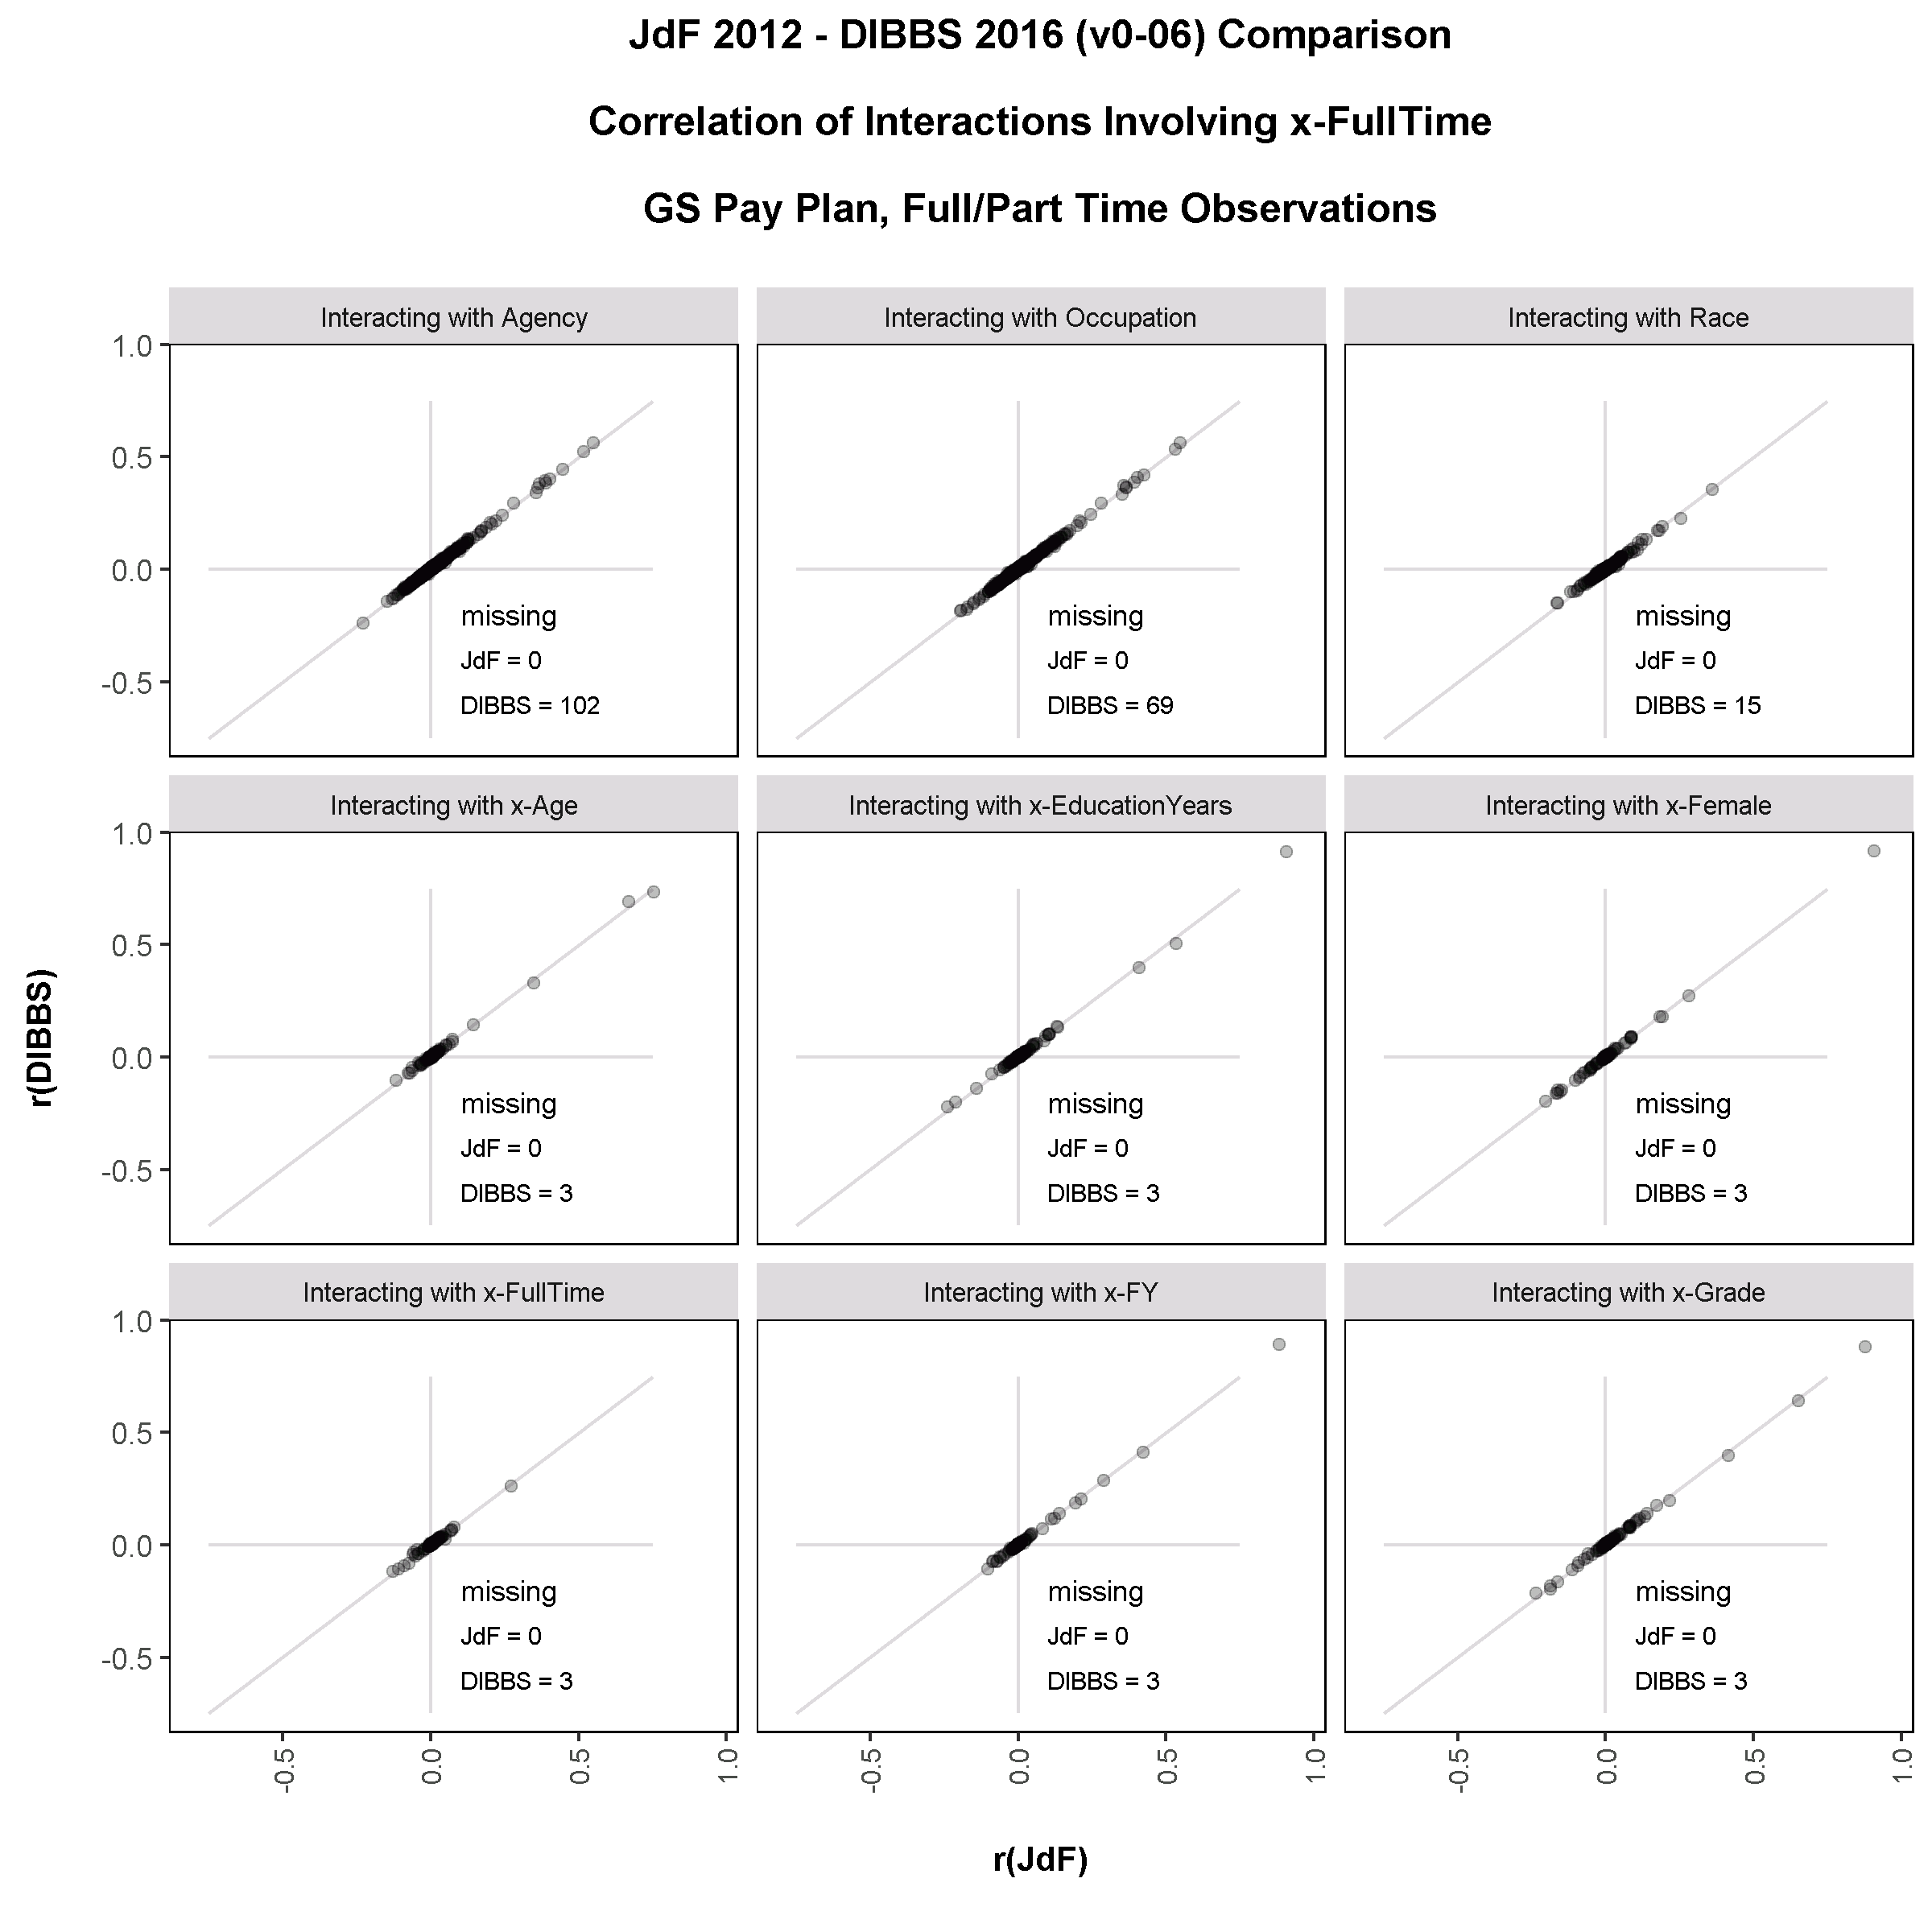
\includegraphics[width=4.5in, trim={0 0.2in 0 1in}, clip]{JdFDIBBSCorrelationInteraction-x-FullTime.png}
        \caption{Correlations involving work schedule}
        \vspace{12pt}
    \end{subfigure}
    \caption{Correlation of primary variables with two variable interactions.  Variable set five.  Synthetic level correlation on y-axis, corresponding authentic correlation on x-axis.}
    \label{figure:JdFDIBBSCorrelationInteraction5}
\end{figure}  

\clearpage

\section{Cumulative Mass (Proportion Observations) by Pay Plan and Occupation}

Pay plan and occupation characterize an employee's job classification and services performed, making them important identifiers in human capital research.  Figures \ref{figure:CMFOccupationPayPlan1} and \ref{figure:CMFOccupationPayPlan2} contain example cumulative mass plots for joint combinations of pay plan and occupation.  All occupations within each pay plan are represented.  Solid line for authentic data, dashed line for synthetic.  ``nJ" indicates observation count in authentic data, ``nD" indicates synthetic data observation count.\\

Observations:  Overlapping or nearness of lines indicates equality of cumulative mass for corresponding levels of occupation within pay plan.  Near identical distribution is observed for high frequency pay plans GS, WG, GM, and VN, which account for more than 95\% of observations, indicating overall close agreement between data sets.  Increasing departure observed as number of observations decreases.\\

\begin{figure}[h!]
    \centering
    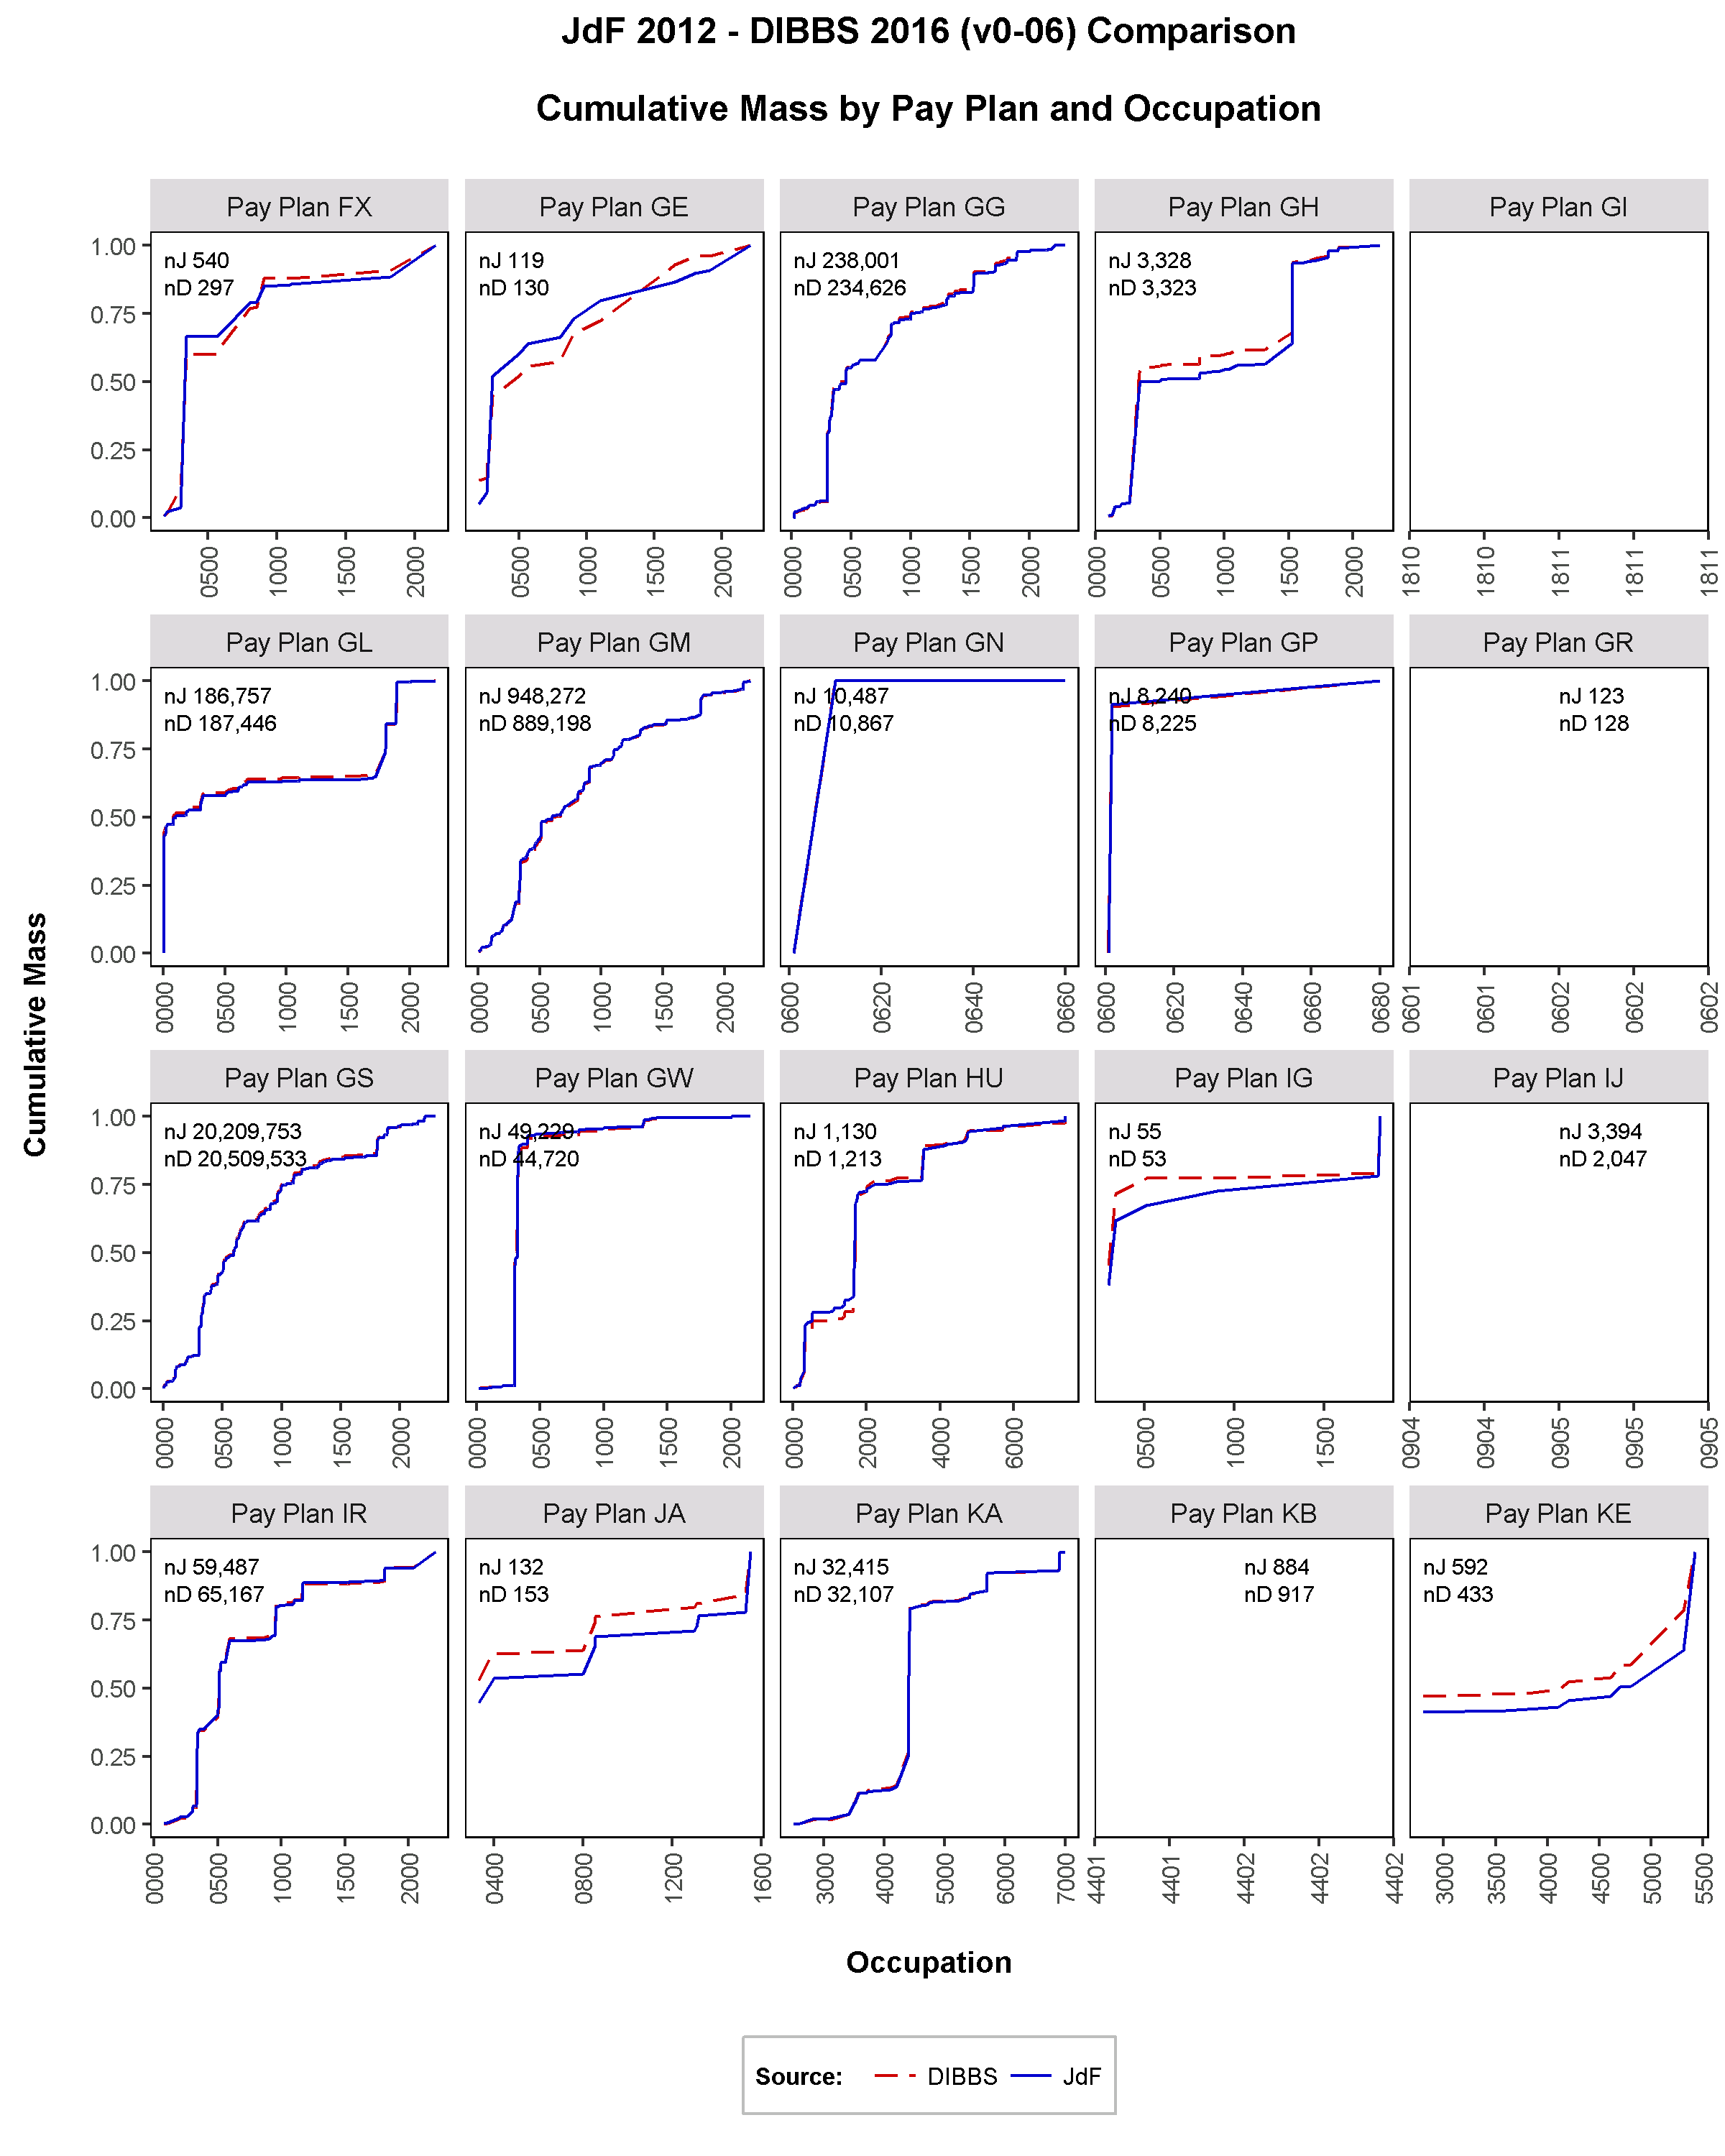
\includegraphics[width=5.85in, trim={0 0.75in 0 0.75in}, clip]{CMFOccupationPayPlan61.png}
    \caption{Cumulative mass (observations) by occupation within pay plan.  Pay plan set one.  Synthetic data represented by dashed line, authentic by solid line.  Occupation on x-axis.}
    \label{figure:CMFOccupationPayPlan1}
\end{figure}

\clearpage

\begin{figure}[]
    \centering
    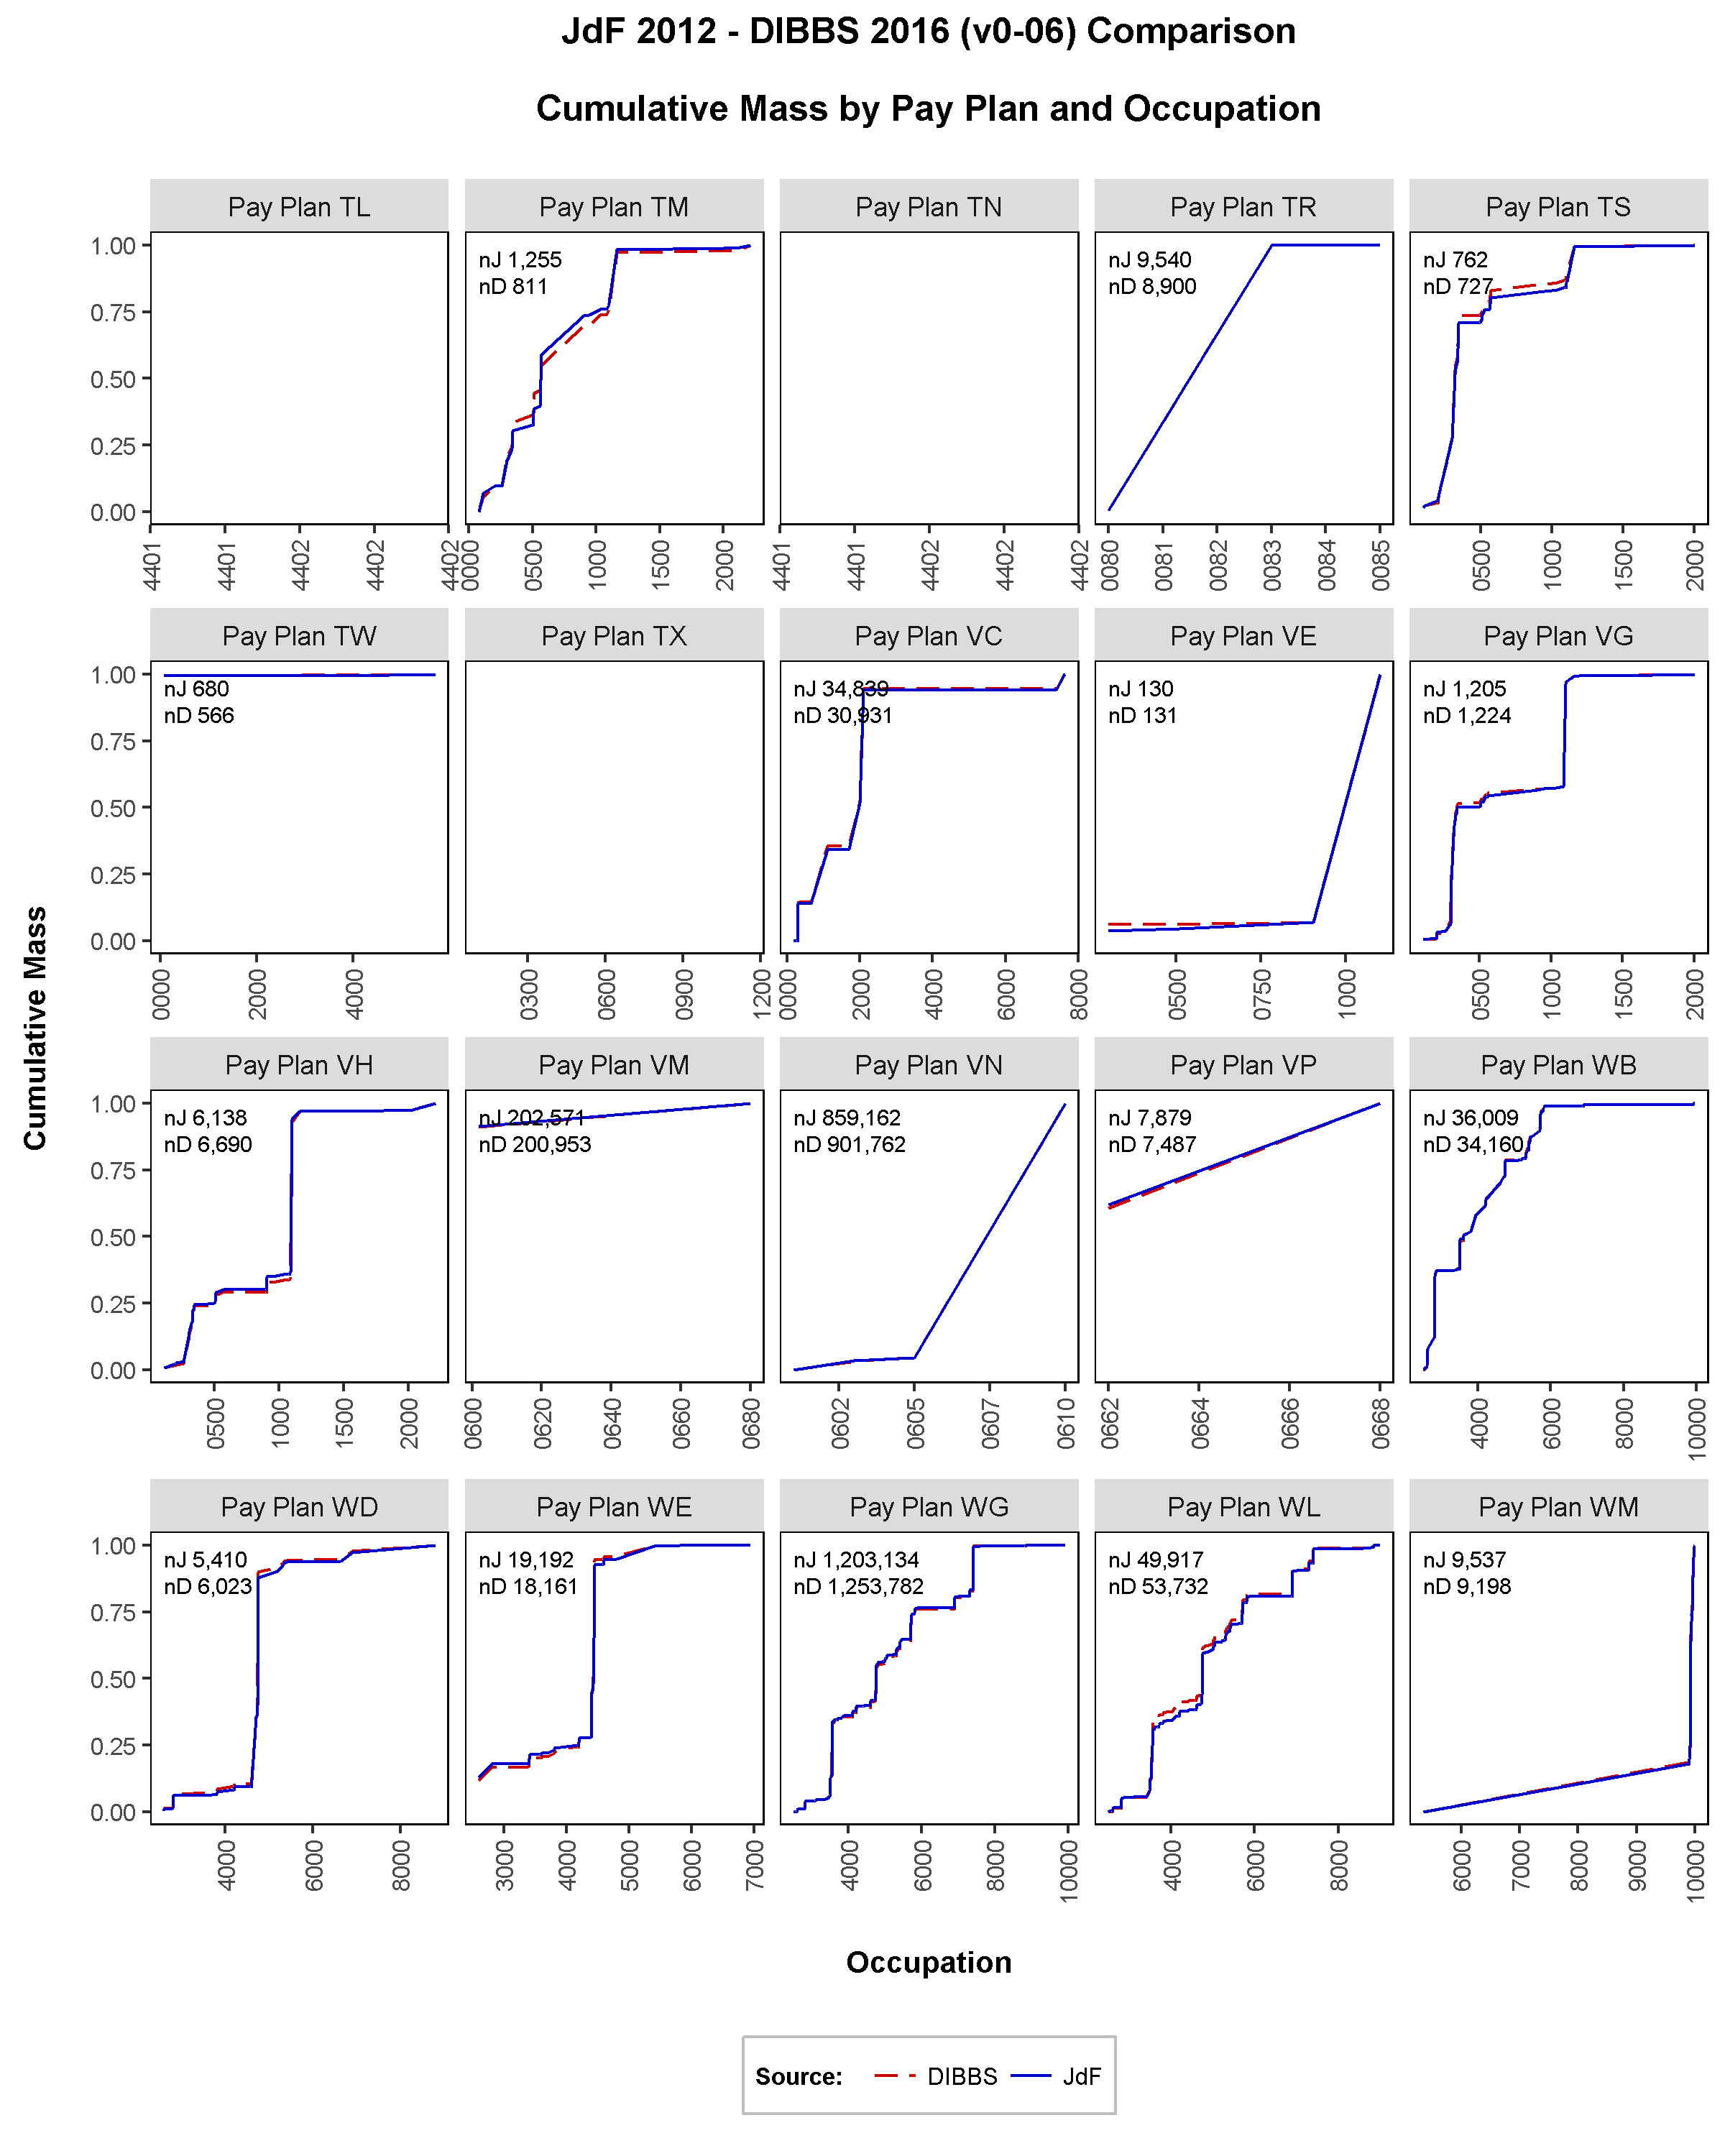
\includegraphics[width=5.85in, trim={0 0.75in 0 0.75in}, clip]{CMFOccupationPayPlan141.png}
    \caption{Cumulative mass (observations) by occupation within pay plan.  Pay plan set two. Synthetic data represented by dashed line, authentic by solid line.  Occupation on x-axis.}
    \label{figure:CMFOccupationPayPlan2}
\end{figure}

\clearpage

\section{Distribution of Grade by Joint Combinations of Agency, Occupation, Education, and Supervisor Status}

Federal employee pay classification consists of a pay plan, grade, and step rate.  Since employee pay is largely determined by grade and promotions are detected by change in grade, it is important for the synthetic data to accurately reflect authentic proportions of observations by grade within joint combinations of critical human capital variables.\footnote{Although pay rate schedules exist for each pay plan, exceptions to published rates of pay may apply when an employee is transferred into a position that requires a grade adjustment.}  Observations are limited to GS pay plan, full-time.\\

Figure \ref{figure:JdFDIBBSGSFullTimeGradeAdminProfessionalAgency} compares synthetic and authentic observation frequencies within joint categories of agency, occupational category, and grade.  Administrative and professional occupational categories are combined and appear in the lower plot of the panel and remaining GS categories (technical, clerical, and other white collar) appear as a group in the upper plot.  Each agency (x-axis) has two columns of dots, one on the left for authentic data and one on the right for synthetic data.  The size of each dot is scaled to represent the number of observations in the corresponding grade listed on the y-axis.  Dot sizes range from small (less than 1,000 observations) to large (more than 250,000 observations).  Total observation counts by agency are listed in rows at the top of each plot, ``n(JdF)" indicating authentic observations, ``n(DIBBS)" indicating synthetic.  Note that the graphs shown are for a sequence of representative agencies.  Those for remaining agencies show similar patterns.\\

Figure \ref{figure:JdFDIBBSGSFullTimeGradeCollegeAgency} compares synthetic and authentic observation frequencies within joint categories of agency, education level (college or not), and grade.  Graphs shown are for a sequence of representative agencies.  Those for remaining agencies show similar patterns.\\

Figure \ref{figure:JdFDIBBSGSFullTimeGradeSupervisoryStatusAgency} compares synthetic and authentic observation frequencies within joint categories of agency, supervisor status, and grade.  Graphs shown are for a sequence of representative agencies.  Those for remaining agencies show similar patterns.\\

Figure \ref{figure:JdFDIBBSGSFullTimeGradeAdminProfessionalOccupation} compares synthetic and authentic observation frequencies within joint categories of occupation, occupational category, and grade.  Since most occupations are restricted to a single occupational category, panels appear disjoint, showing observations in one category, but not the other.  Synthetic data frequencies accurately reflect this property.  Graphs shown are for a sequence of representative occupations.  Those for remaining occupations show similar patterns.\\

Figure \ref{figure:JdFDIBBSGSFullTimeGradeCollegeOccupation} compares synthetic and authentic observation frequencies within joint categories of occupation, education level (college or not), and grade.  Graphs shown are for a sequence of representative occupations.  Those for remaining occupations show similar patterns.\\

Figure \ref{figure:JdFDIBBSGSFullTimeGradeSupervisoryStatusOccupation} compares synthetic and authentic observation frequencies within joint categories of occupation, supervisor status, and grade.  Graphs shown are for a sequence of representative occupations.  Those for remaining occupations show similar patterns.\\

Observations:  Within the resolution of dot size, joint frequencies of agency, occupational category, occupation, education, supervisor status, and grade appear to agree in the data sets.  To compare n(DIBBS) and n(JdF) observation counts (aggregated counts for all grades within category combinations), the ratio of difference in synthetic and authentic count to authentic count was computed.  Figure \ref{figure:nRatioGrade} plots these ratios against corresponding authentic counts (in log scale).  Differences tend to be positive (synthetic greater than authentic) and there is a general decrease in error proportion with increase in n.

\clearpage

\begin{figure}[]
    \centering
    \begin{subfigure}{1\textwidth}
        \centering
        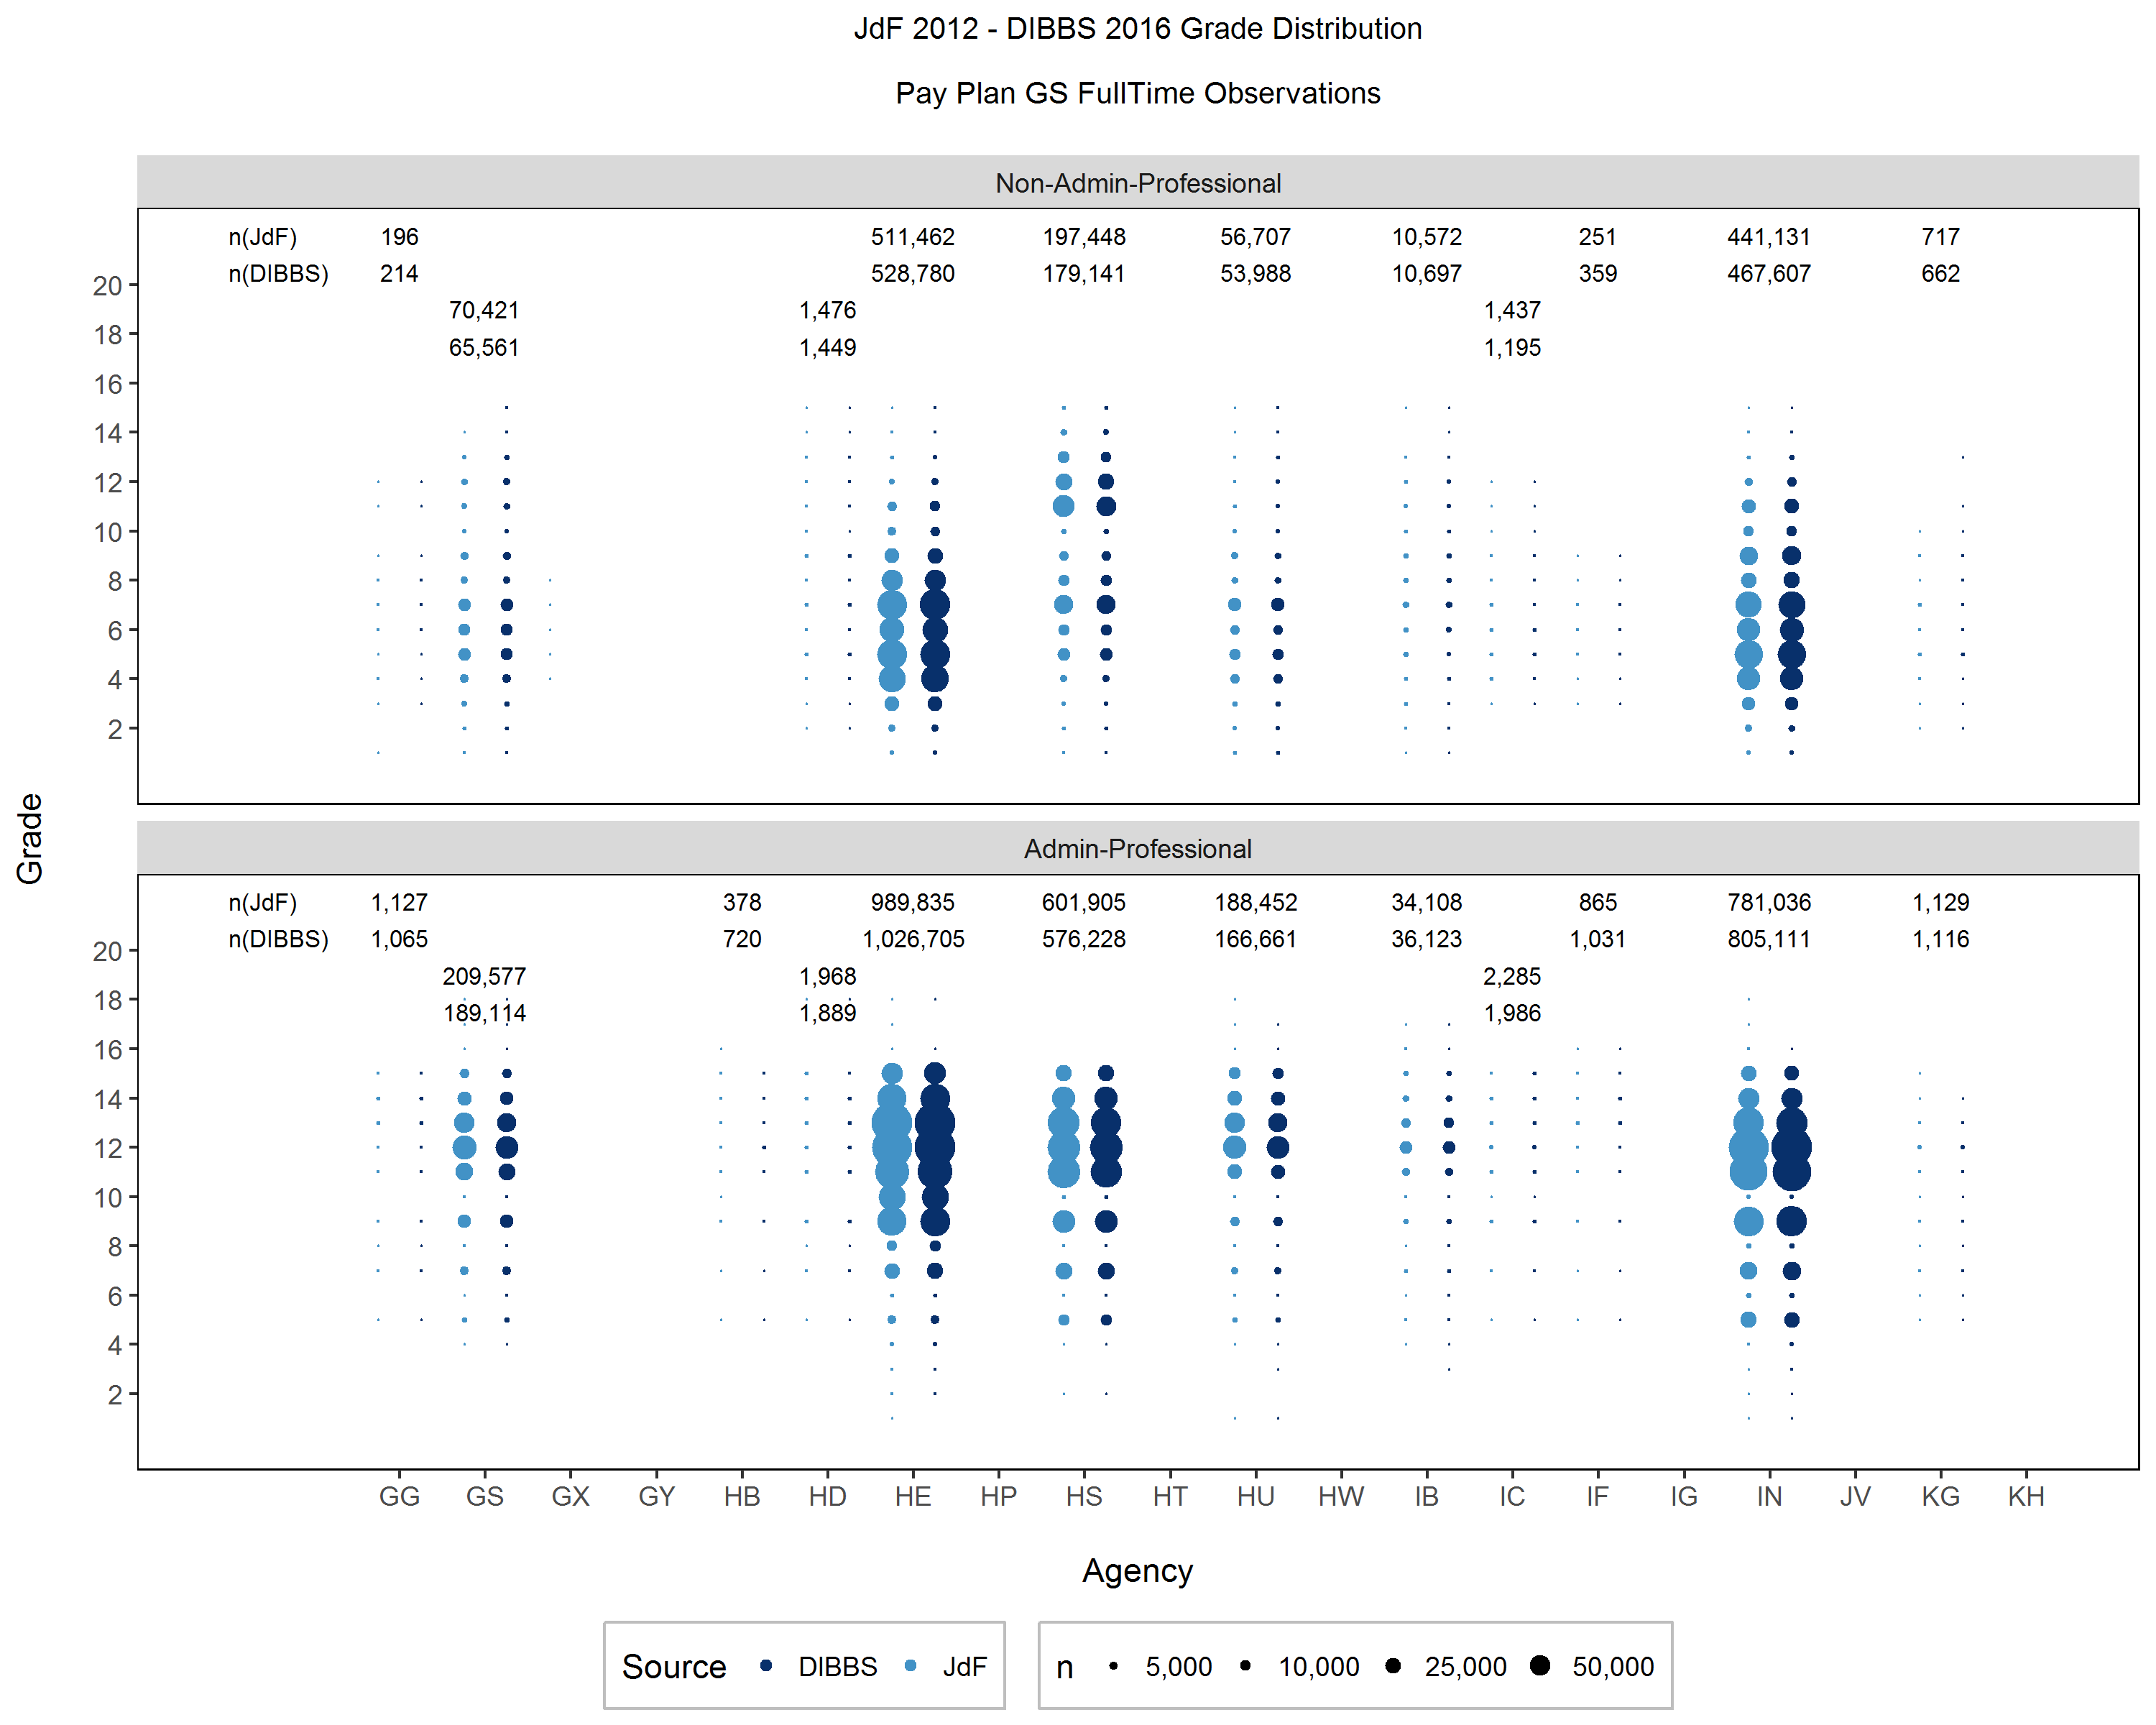
\includegraphics[width=6in, trim={0 200px 0 165px}, clip]{JdFDIBBSGSFullTimeGradeAdminProfessionalAgency61.png}
        \caption{Agencies GG through KH}
        \vspace{20pt}
    \end{subfigure}
    \begin{subfigure}{1\textwidth}
        \centering
        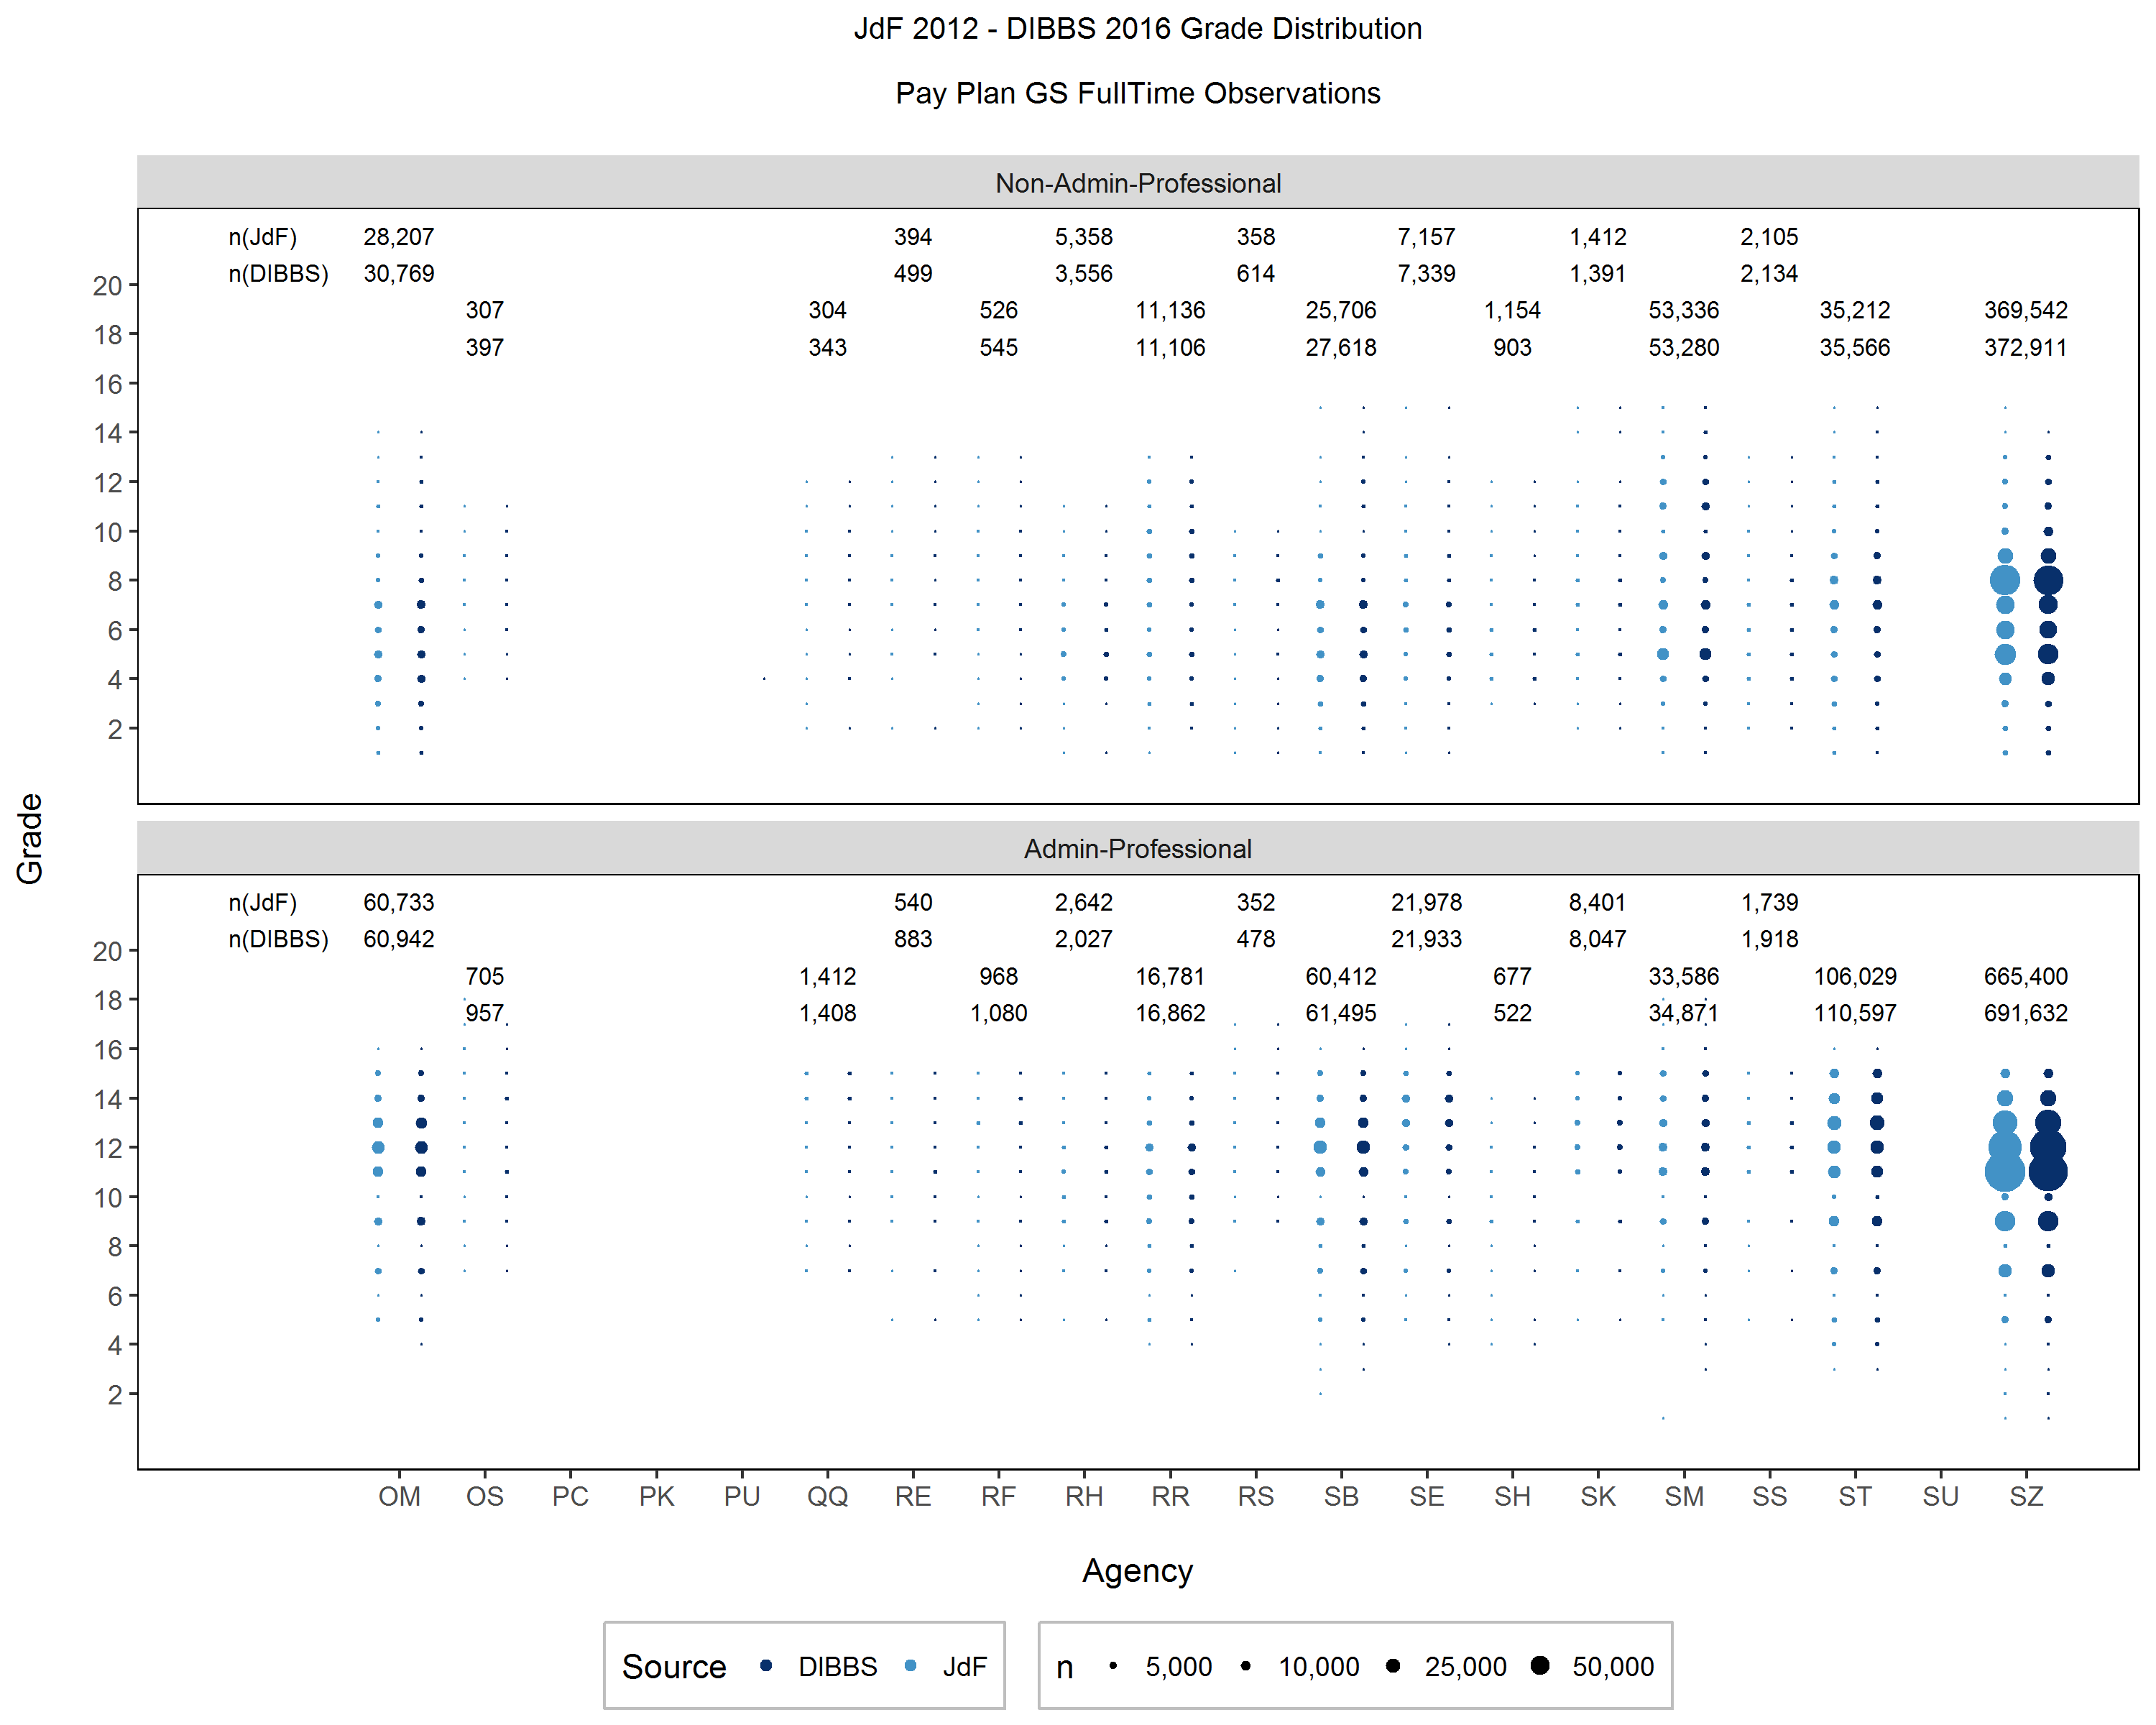
\includegraphics[width=6in, trim={0 200px 0 165px}, clip]{JdFDIBBSGSFullTimeGradeAdminProfessionalAgency101.png}
        \caption{Agencies OM through SZ}
        \vspace{10pt}
    \end{subfigure}
    \caption{Distribution of grade by agency.  Occupational categories Admin/Professional vs. non Admin/Professional.  Authentic on left, synthetic on right.  Dot size small (n$<$5,000) to large (n$>$250,000).  Agencies on x-axis.}
    \label{figure:JdFDIBBSGSFullTimeGradeAdminProfessionalAgency}
\end{figure}

\clearpage

\begin{figure}[]
    \centering
    \begin{subfigure}{1\textwidth}
        \centering
        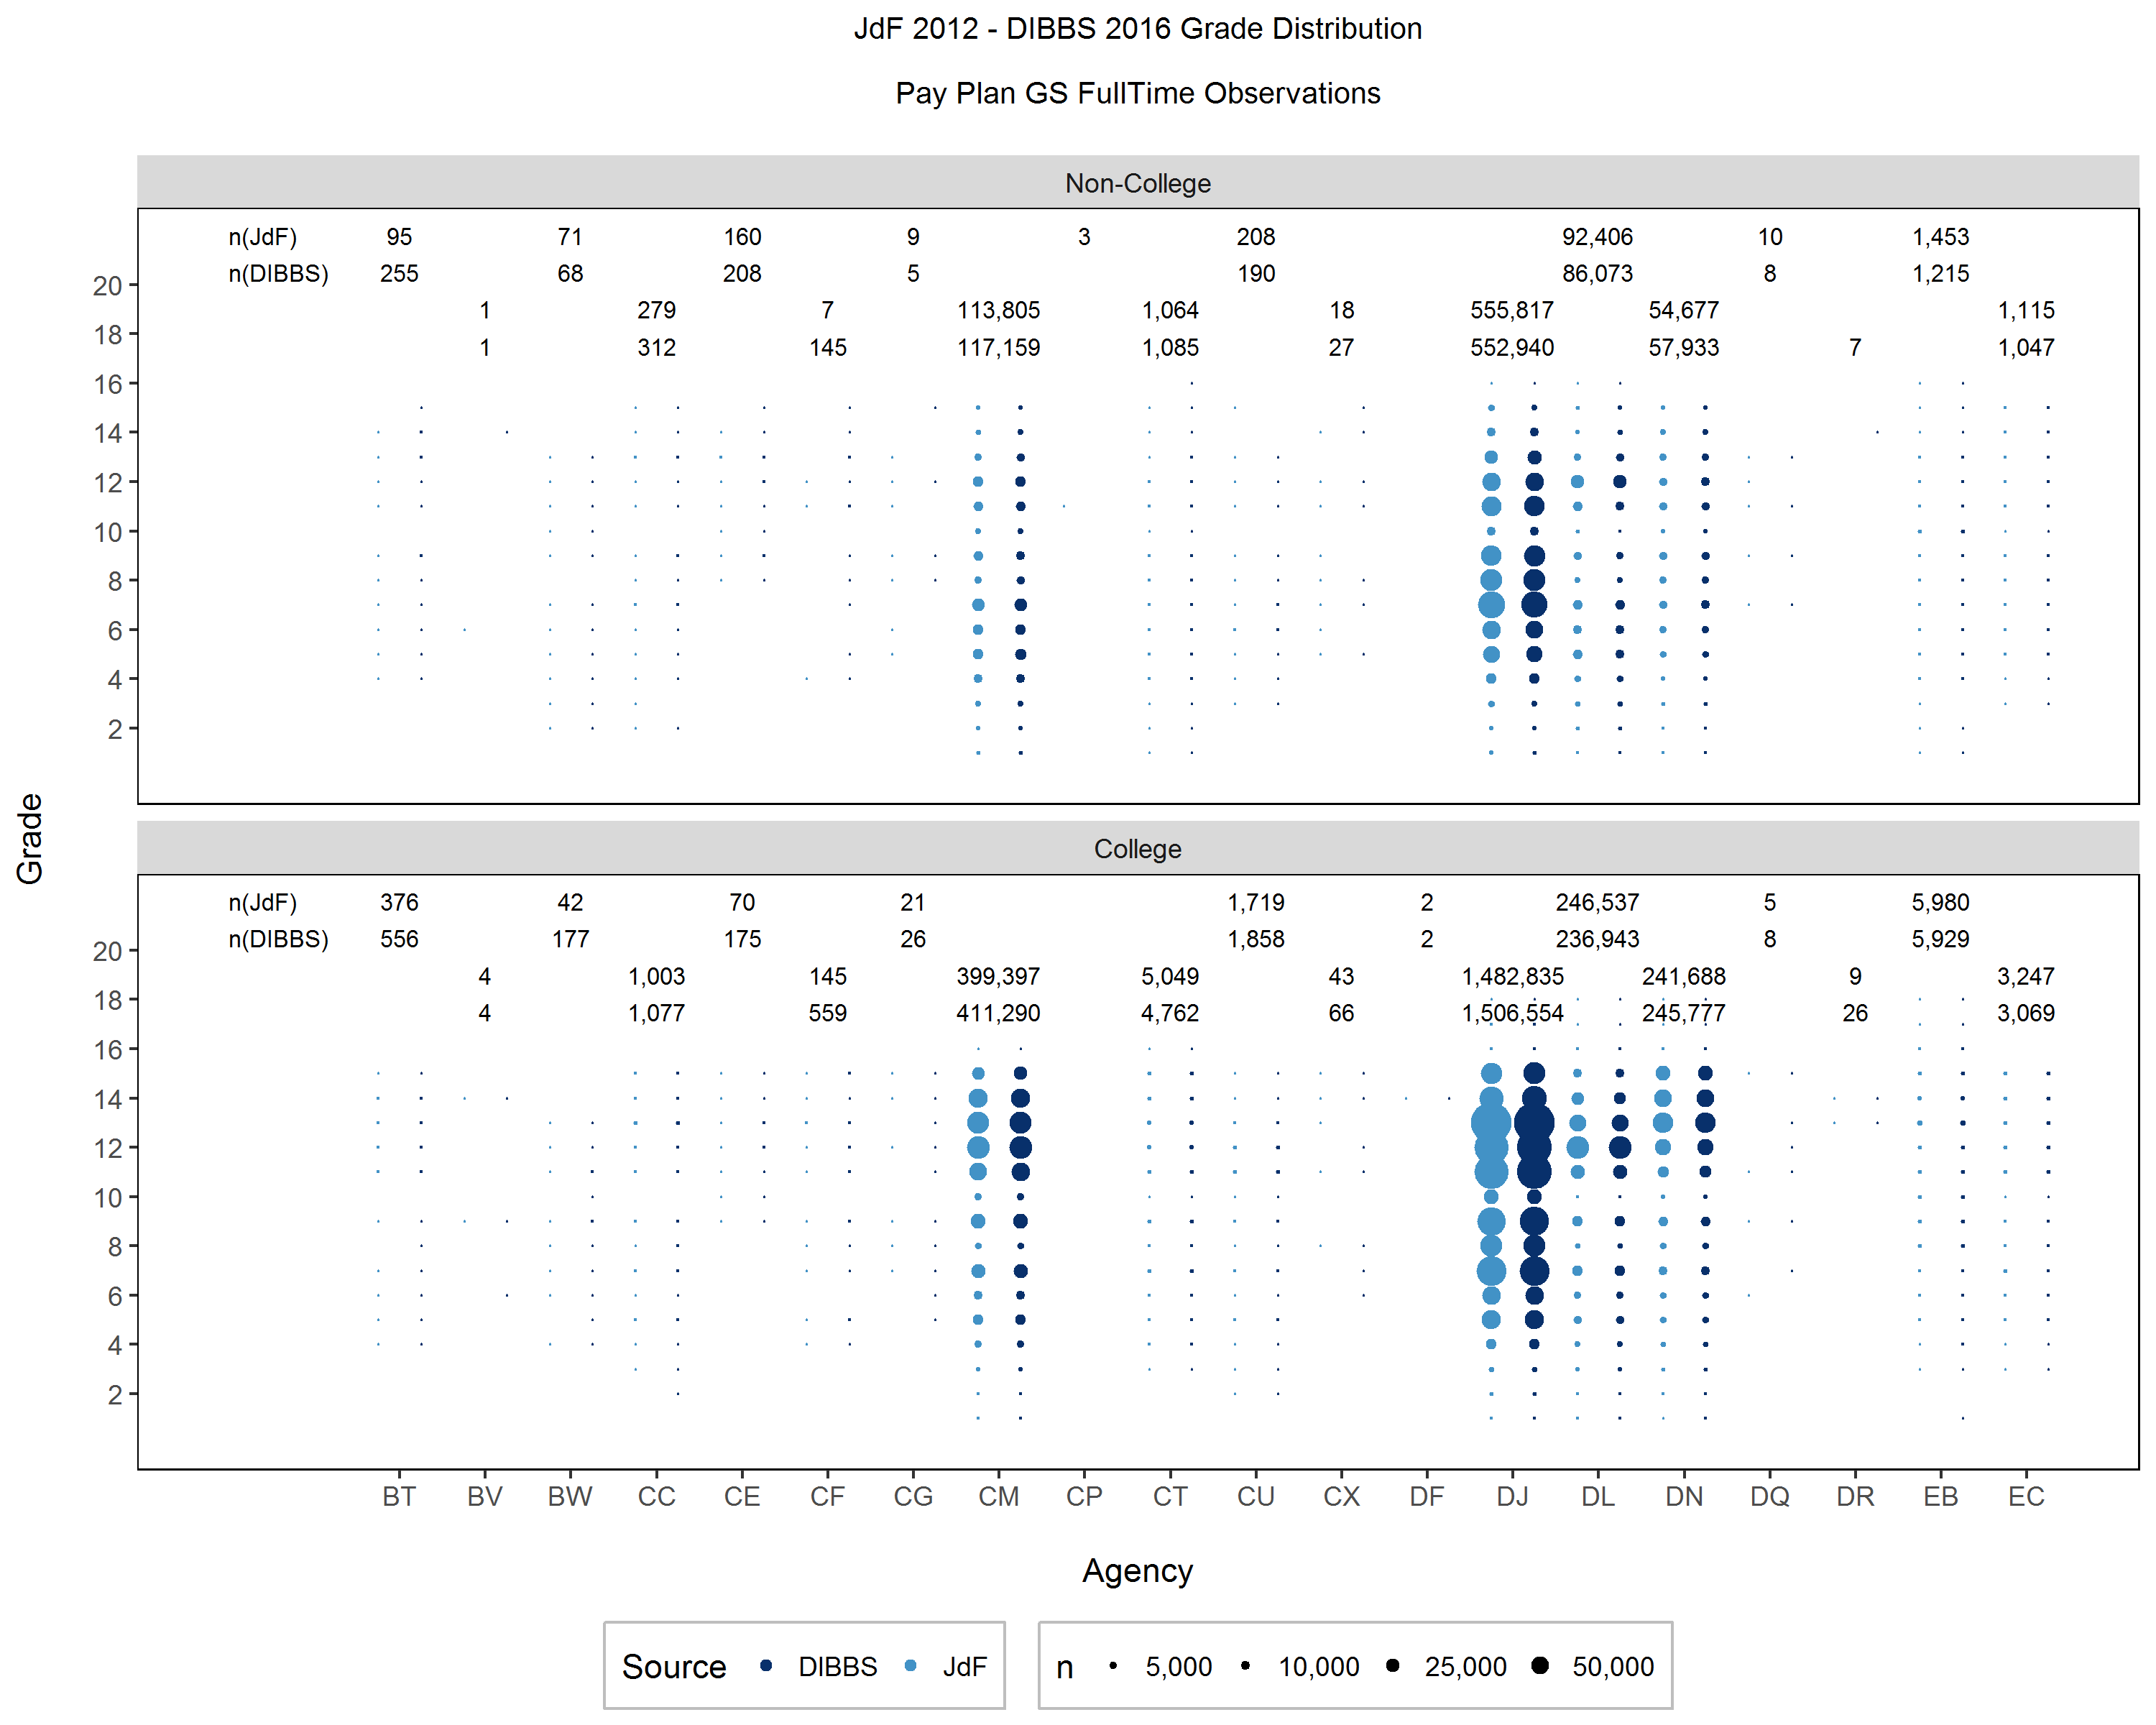
\includegraphics[width=6in, trim={0 200px 0 165px}, clip]{JdFDIBBSGSFullTimeGradeCollegeAgency21.png}
        \caption{Agencies BT through EC}
        \vspace{20pt}
    \end{subfigure}
    \begin{subfigure}{1\textwidth}
        \centering
        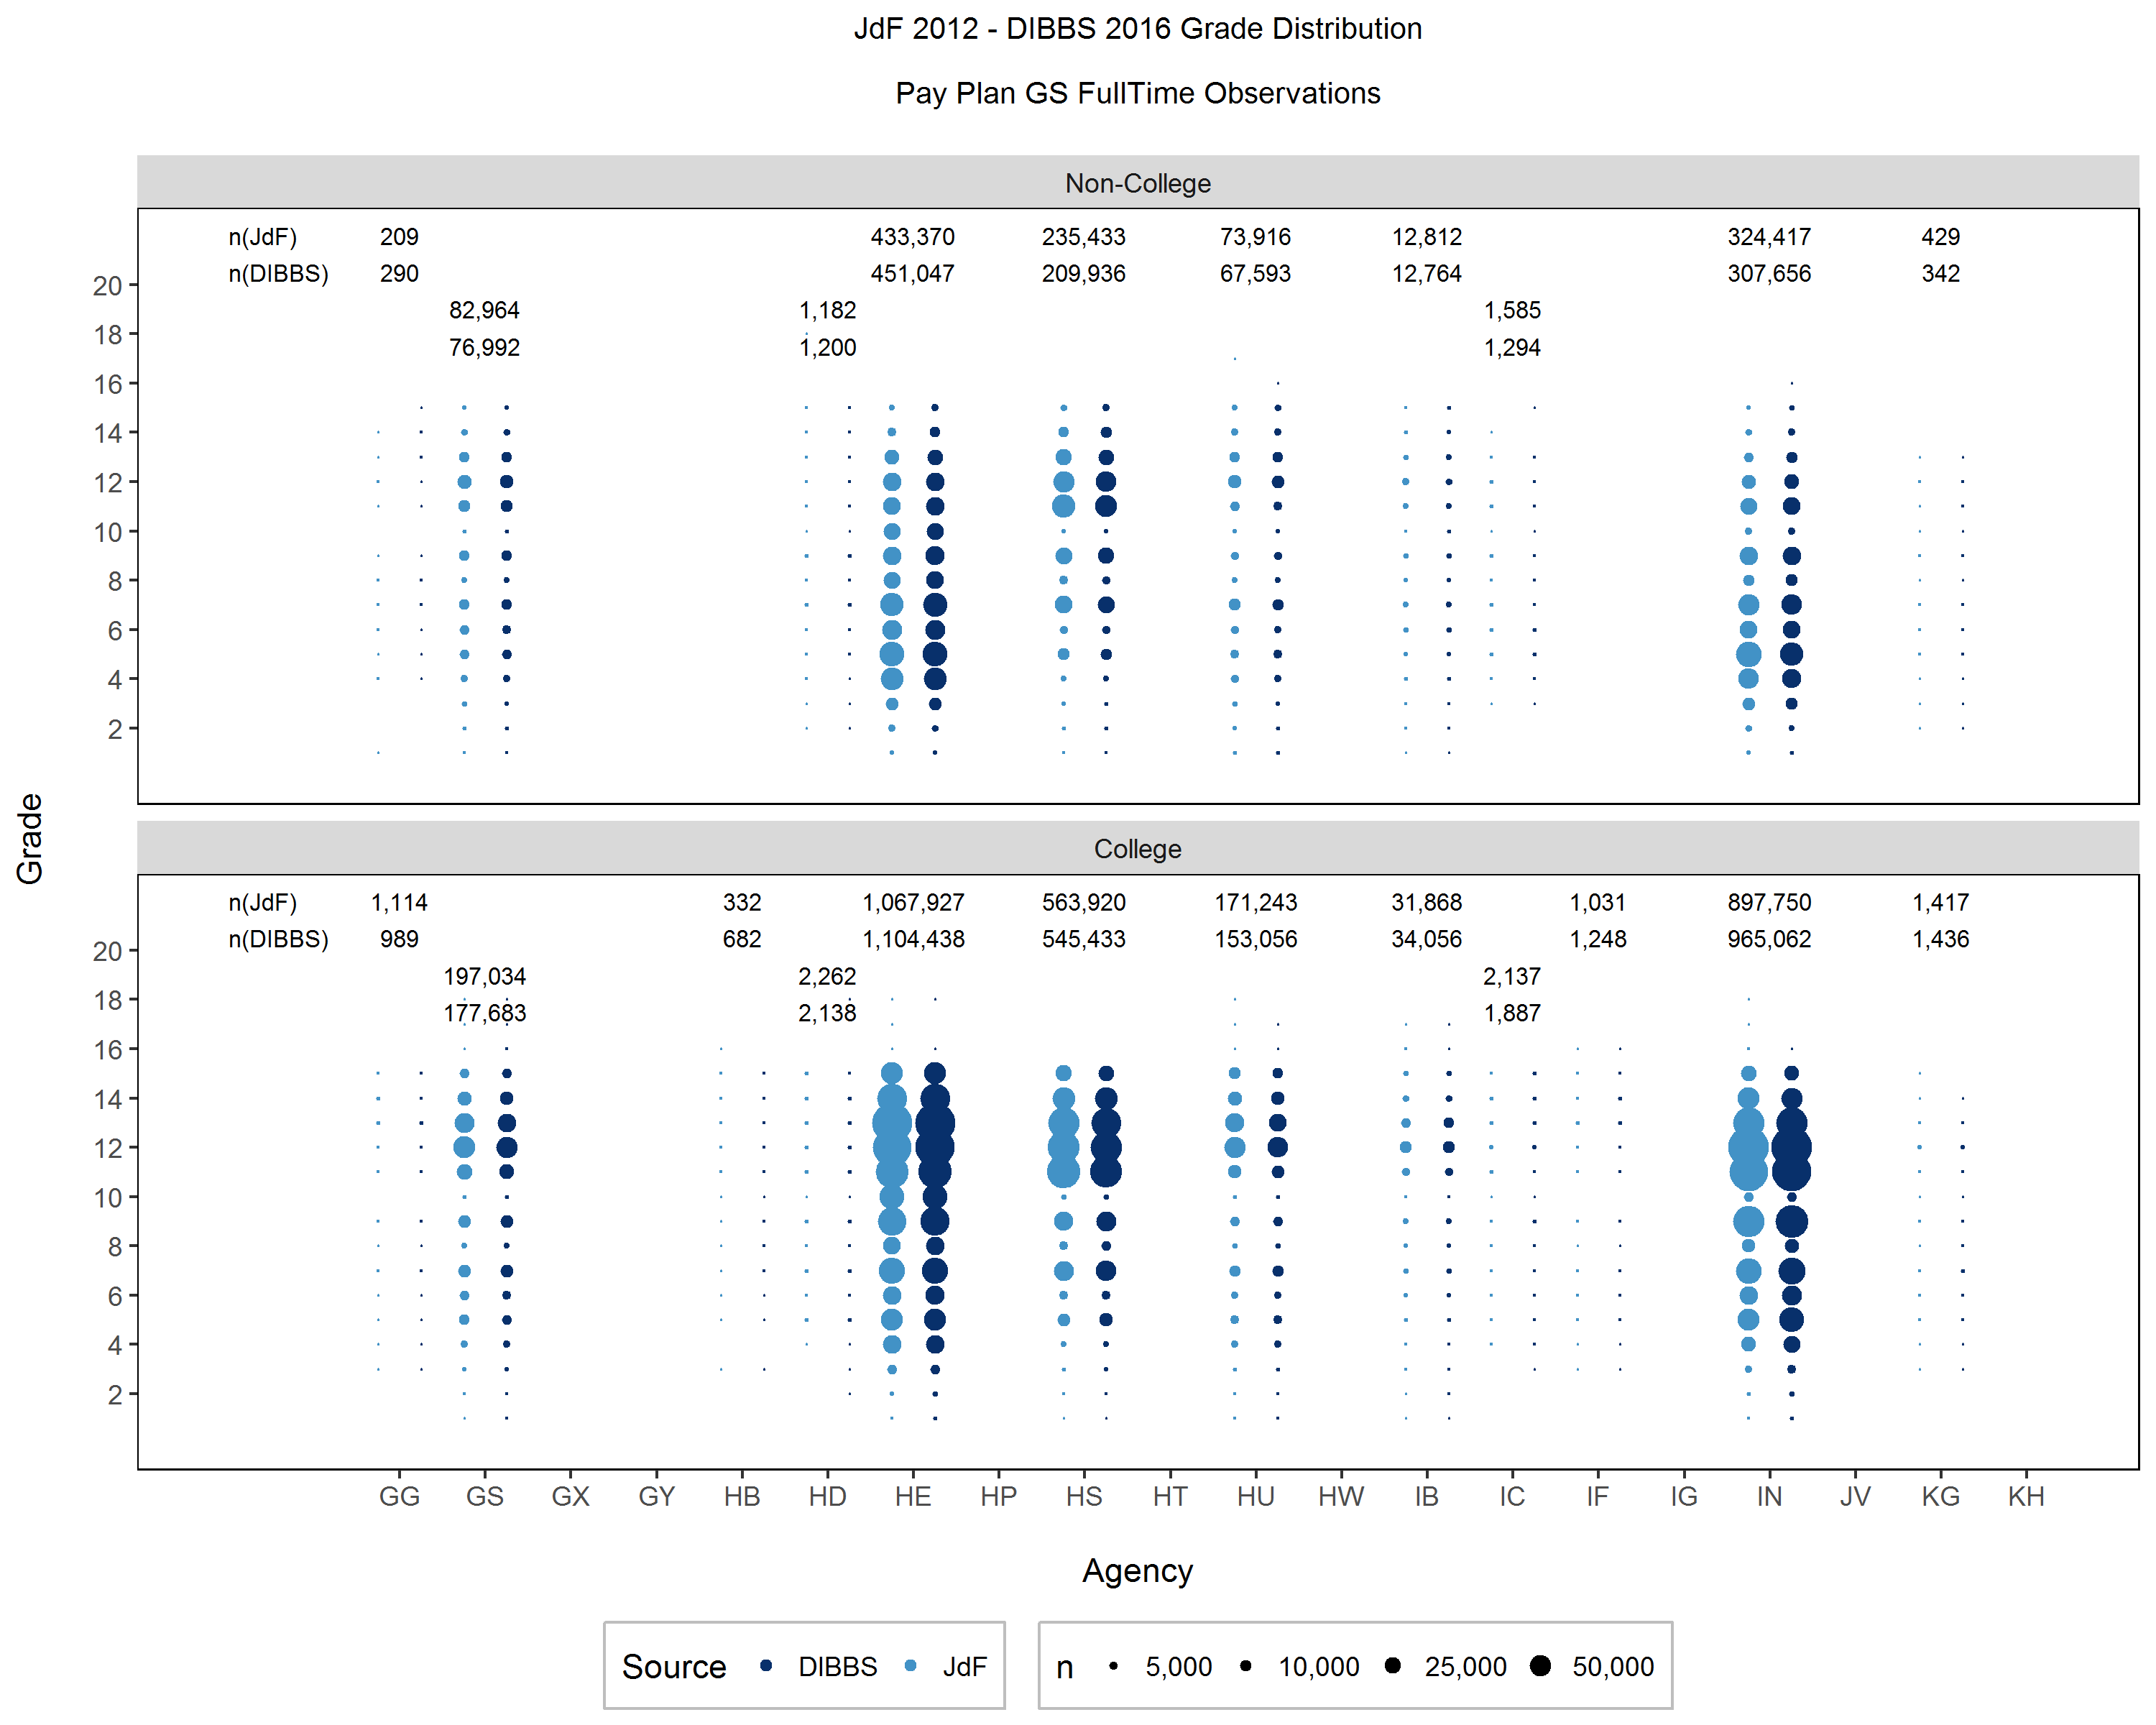
\includegraphics[width=6in, trim={0 200px 0 165px}, clip]{JdFDIBBSGSFullTimeGradeCollegeAgency61.png}
        \caption{Agencies GG through KH}
        \vspace{10pt}
    \end{subfigure}
    \caption{Distribution of grade by agency.  College education vs. non-college.  Authentic on left, synthetic on right.  Dot size small (n$<$5,000) to large (n$>$250,000).  Agencies on x-axis.}
    \label{figure:JdFDIBBSGSFullTimeGradeCollegeAgency}
\end{figure}

\clearpage

\begin{figure}[]
    \centering
    \begin{subfigure}{1\textwidth}
        \centering
        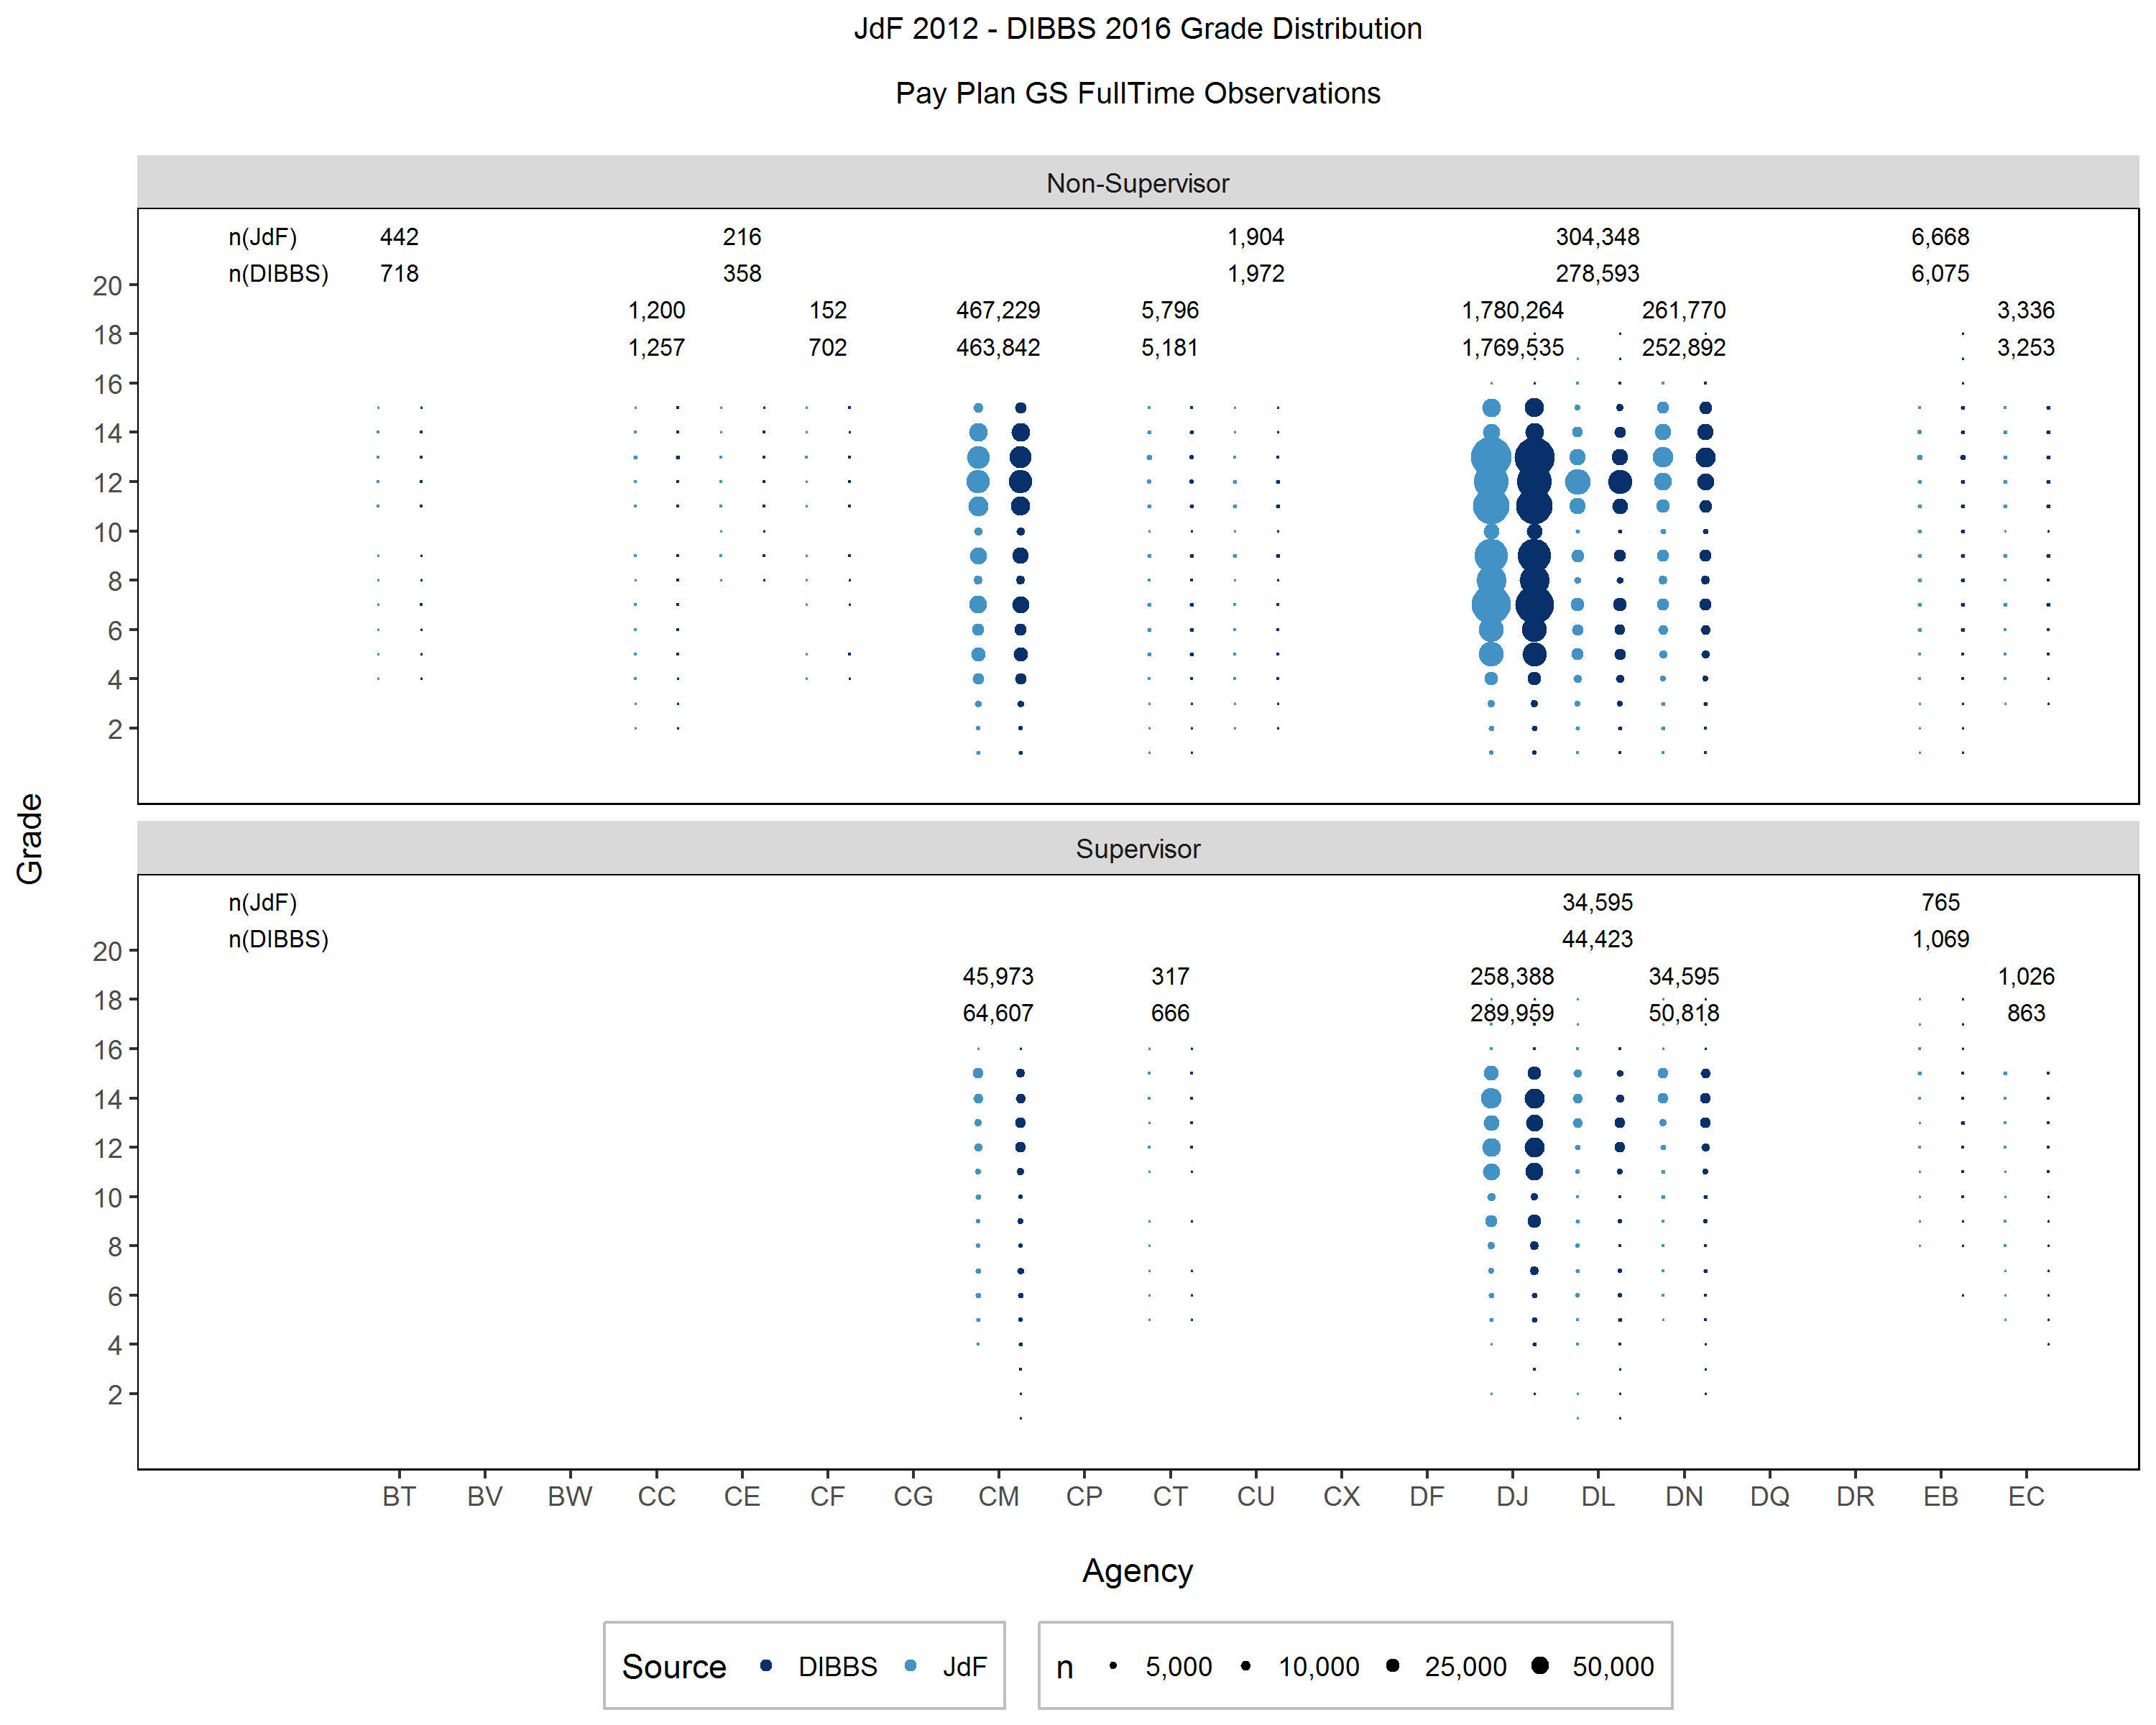
\includegraphics[width=6in, trim={0 200px 0 165px}, clip]{JdFDIBBSGSFullTimeGradeSupervisoryStatusAgency21.png}
        \caption{Agencies BT through EC}
        \vspace{20pt}
    \end{subfigure}
    \begin{subfigure}{1\textwidth}
        \centering
        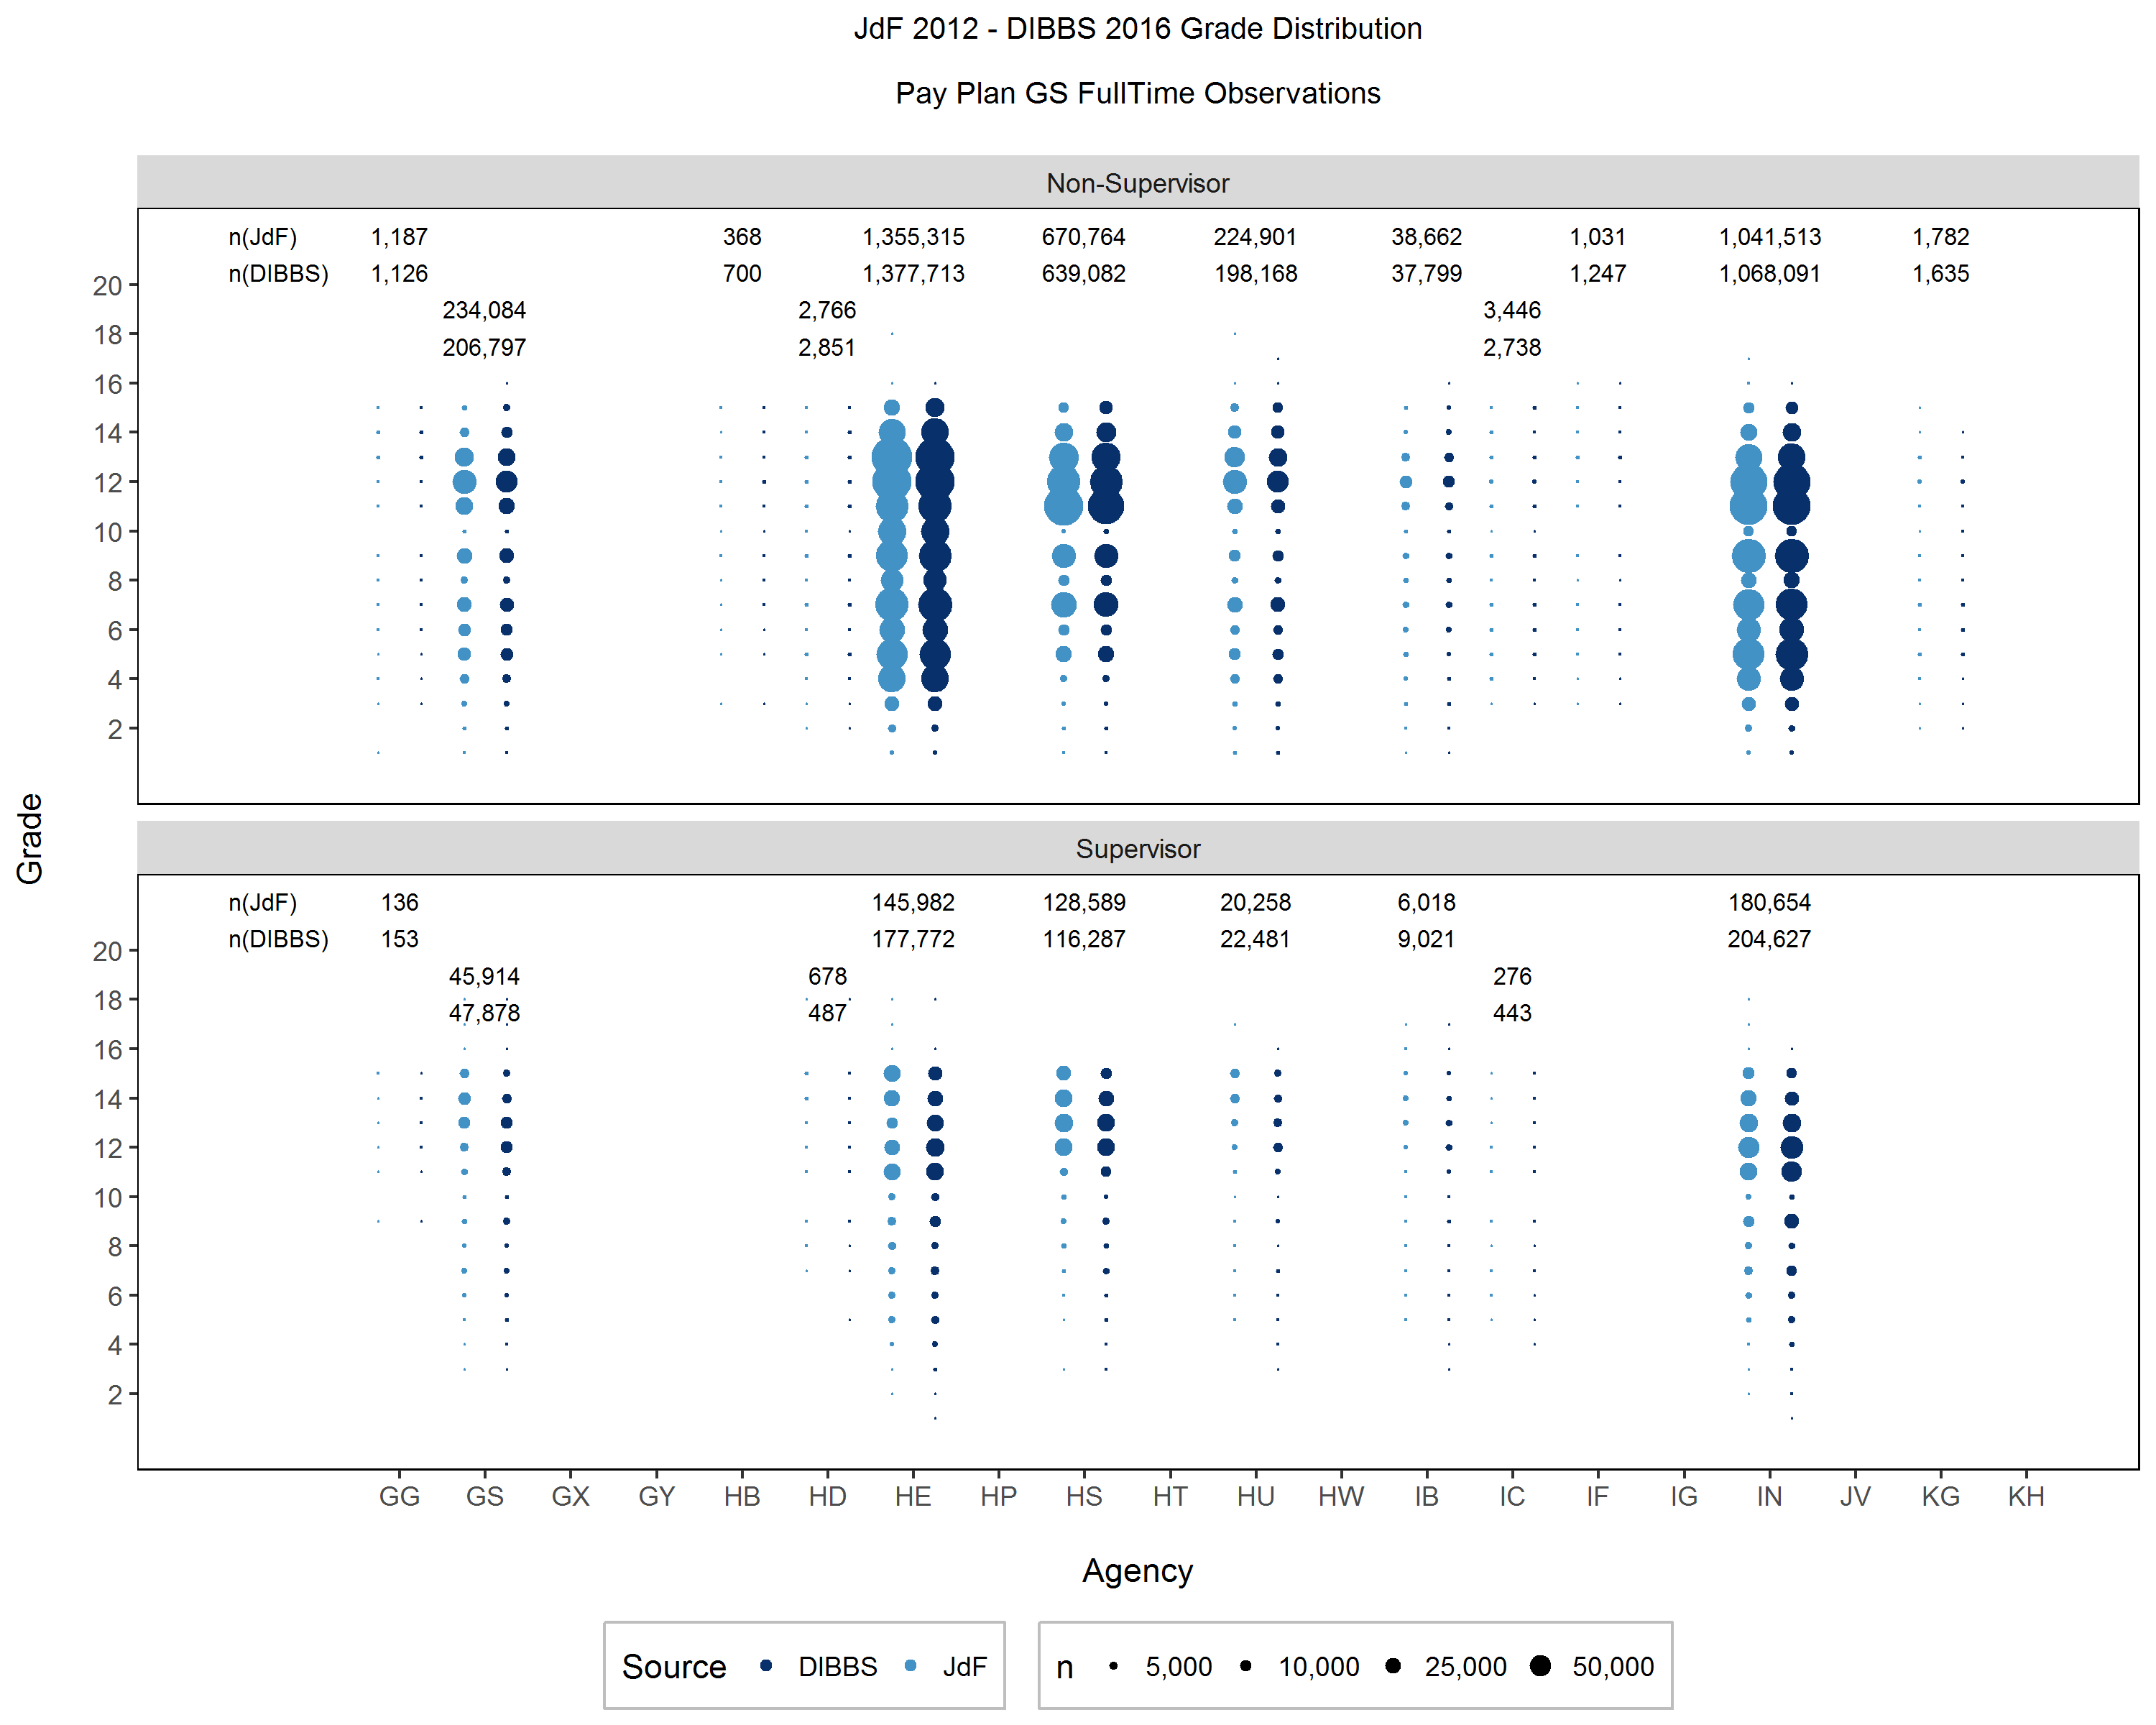
\includegraphics[width=6in, trim={0 200px 0 165px}, clip]{JdFDIBBSGSFullTimeGradeSupervisoryStatusAgency61.png}
        \caption{Agencies GG through KH}
        \vspace{10pt}
    \end{subfigure}
    \caption{Distribution of grade by agency and supervisor status.  Authentic on left, synthetic on right.  Dot size small (n$<$5,000) to large (n$>$250,000).  Agencies on x-axis.}
    \label{figure:JdFDIBBSGSFullTimeGradeSupervisoryStatusAgency}
\end{figure}

\clearpage

\begin{figure}[]
    \centering
    \begin{subfigure}{1\textwidth}
        \centering
        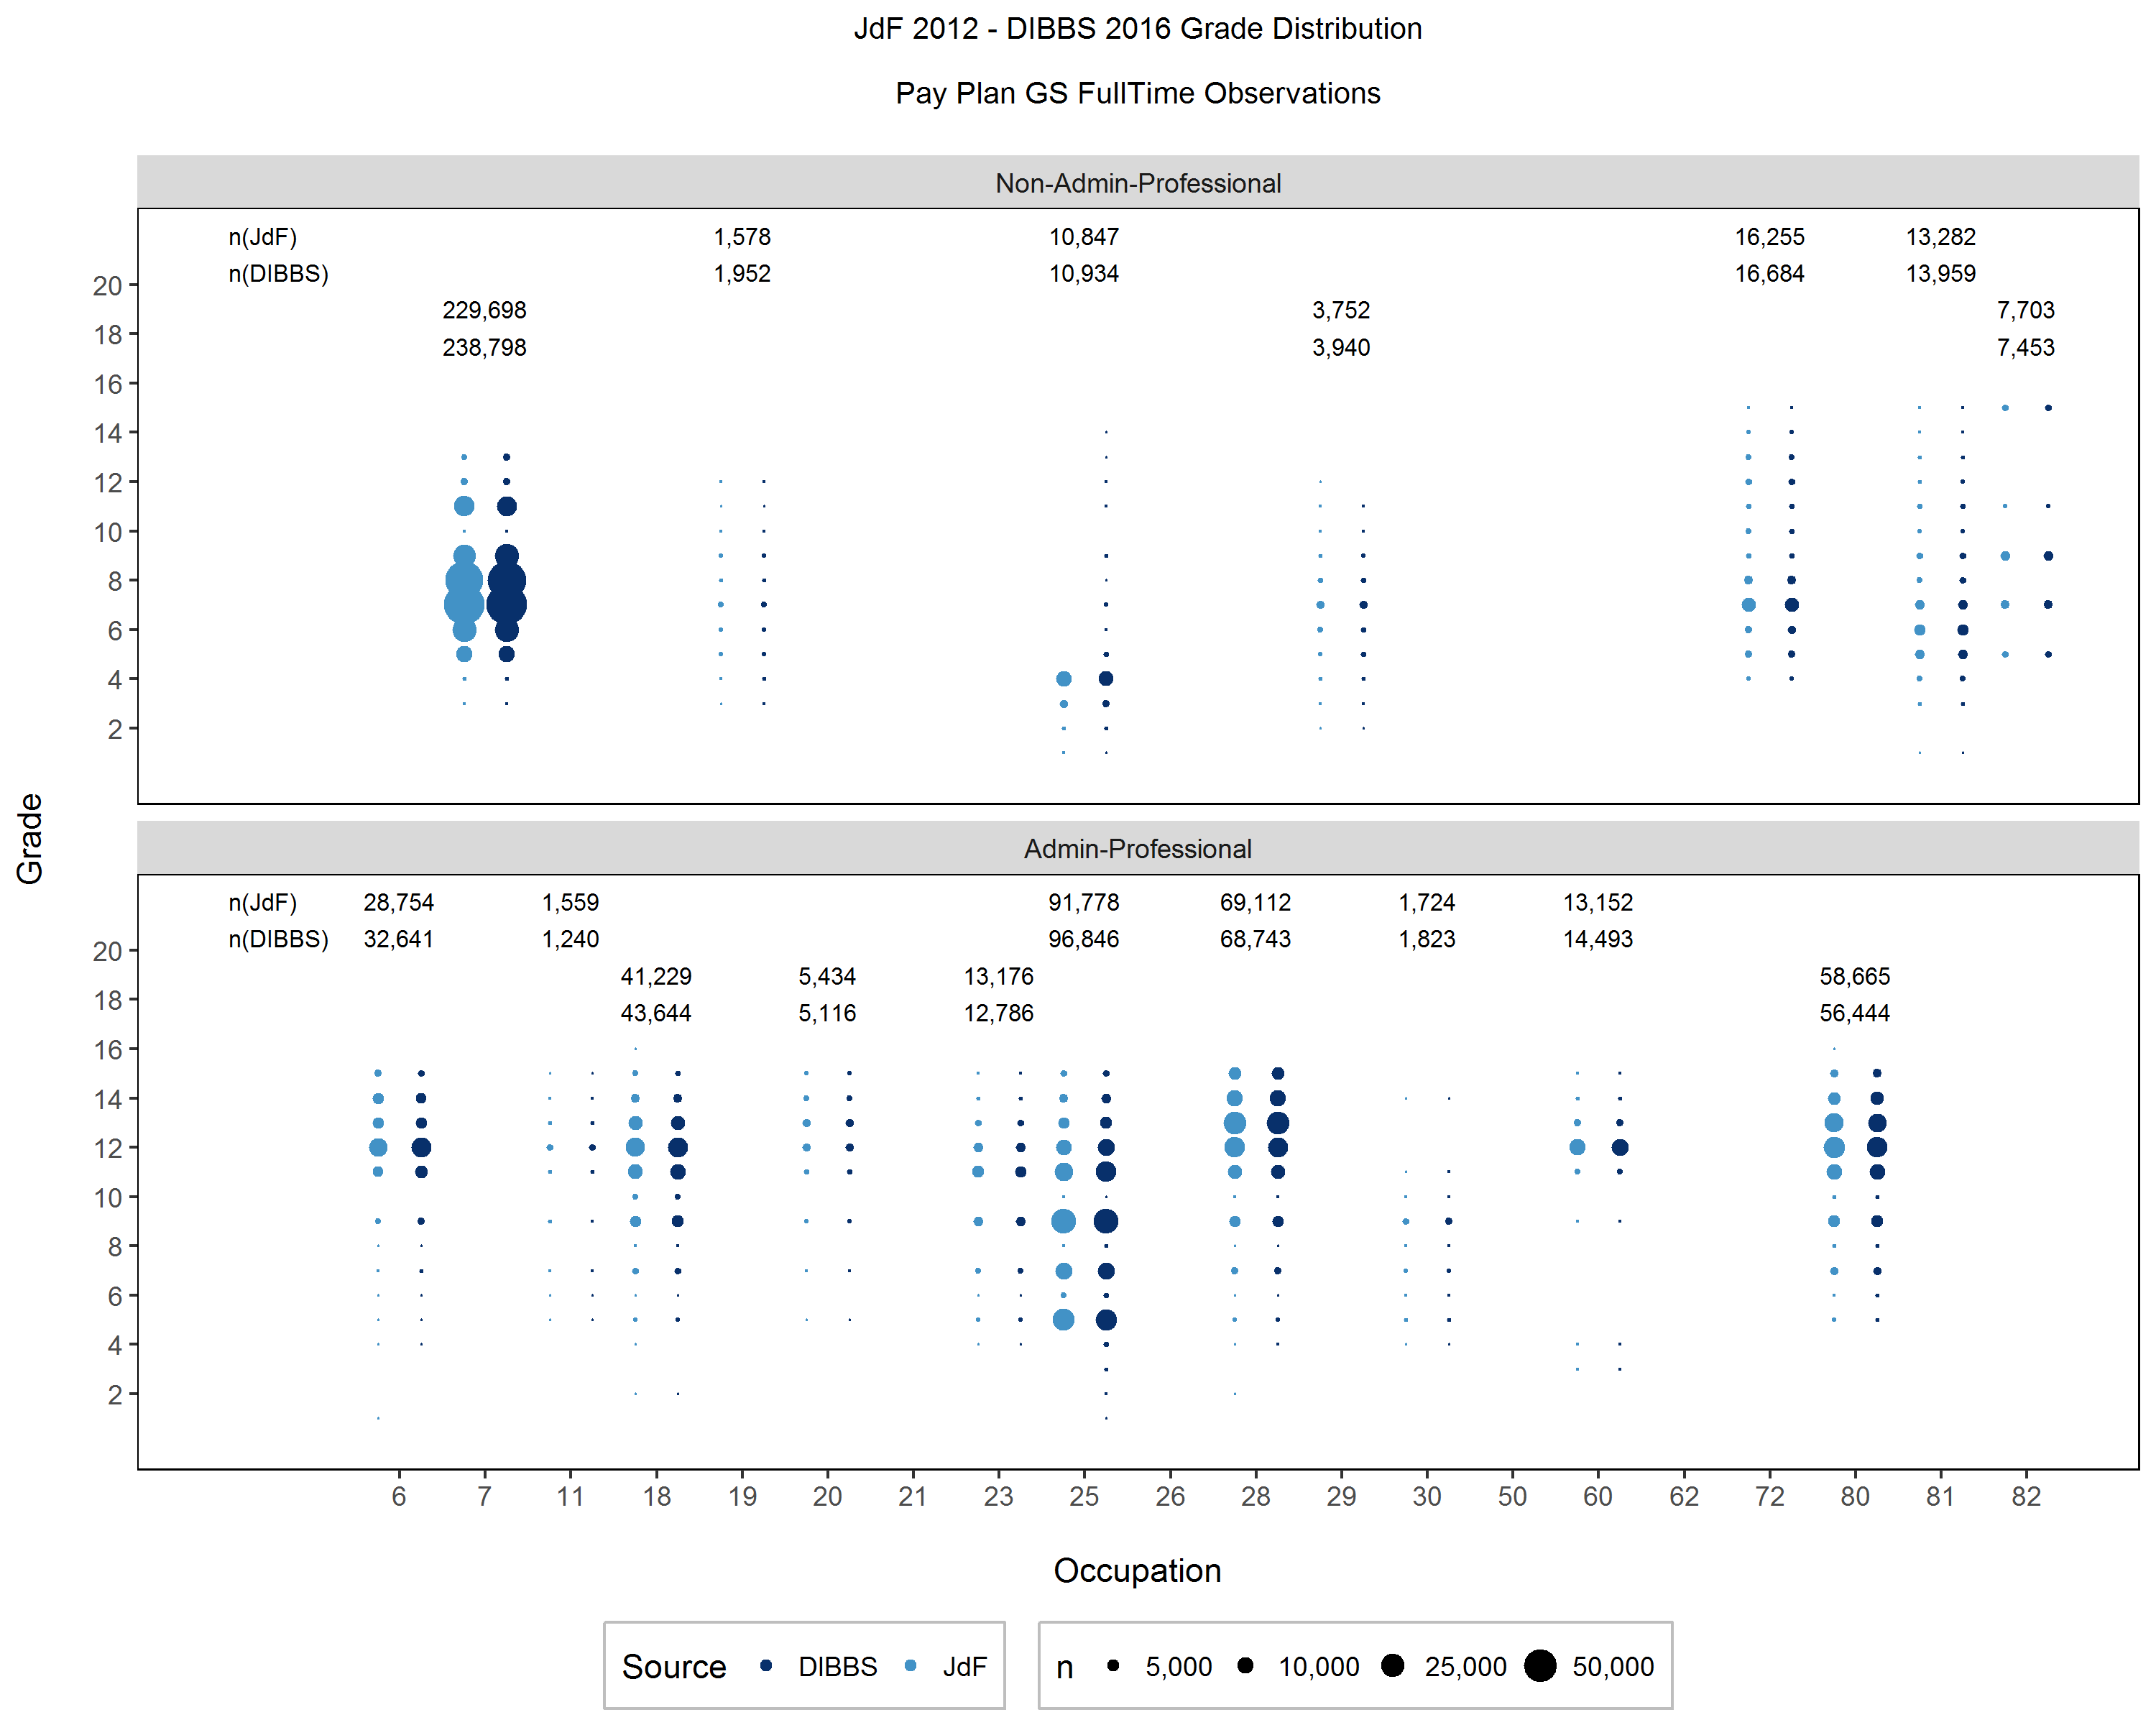
\includegraphics[width=6in, trim={0 200px 0 165px}, clip]{JdFDIBBSGSFullTimeGradeAdminProfessionalOccupation1.png}
        \caption{Occupations 0006 through 0082}
        \vspace{20pt}
    \end{subfigure}
    \begin{subfigure}{1\textwidth}
        \centering
        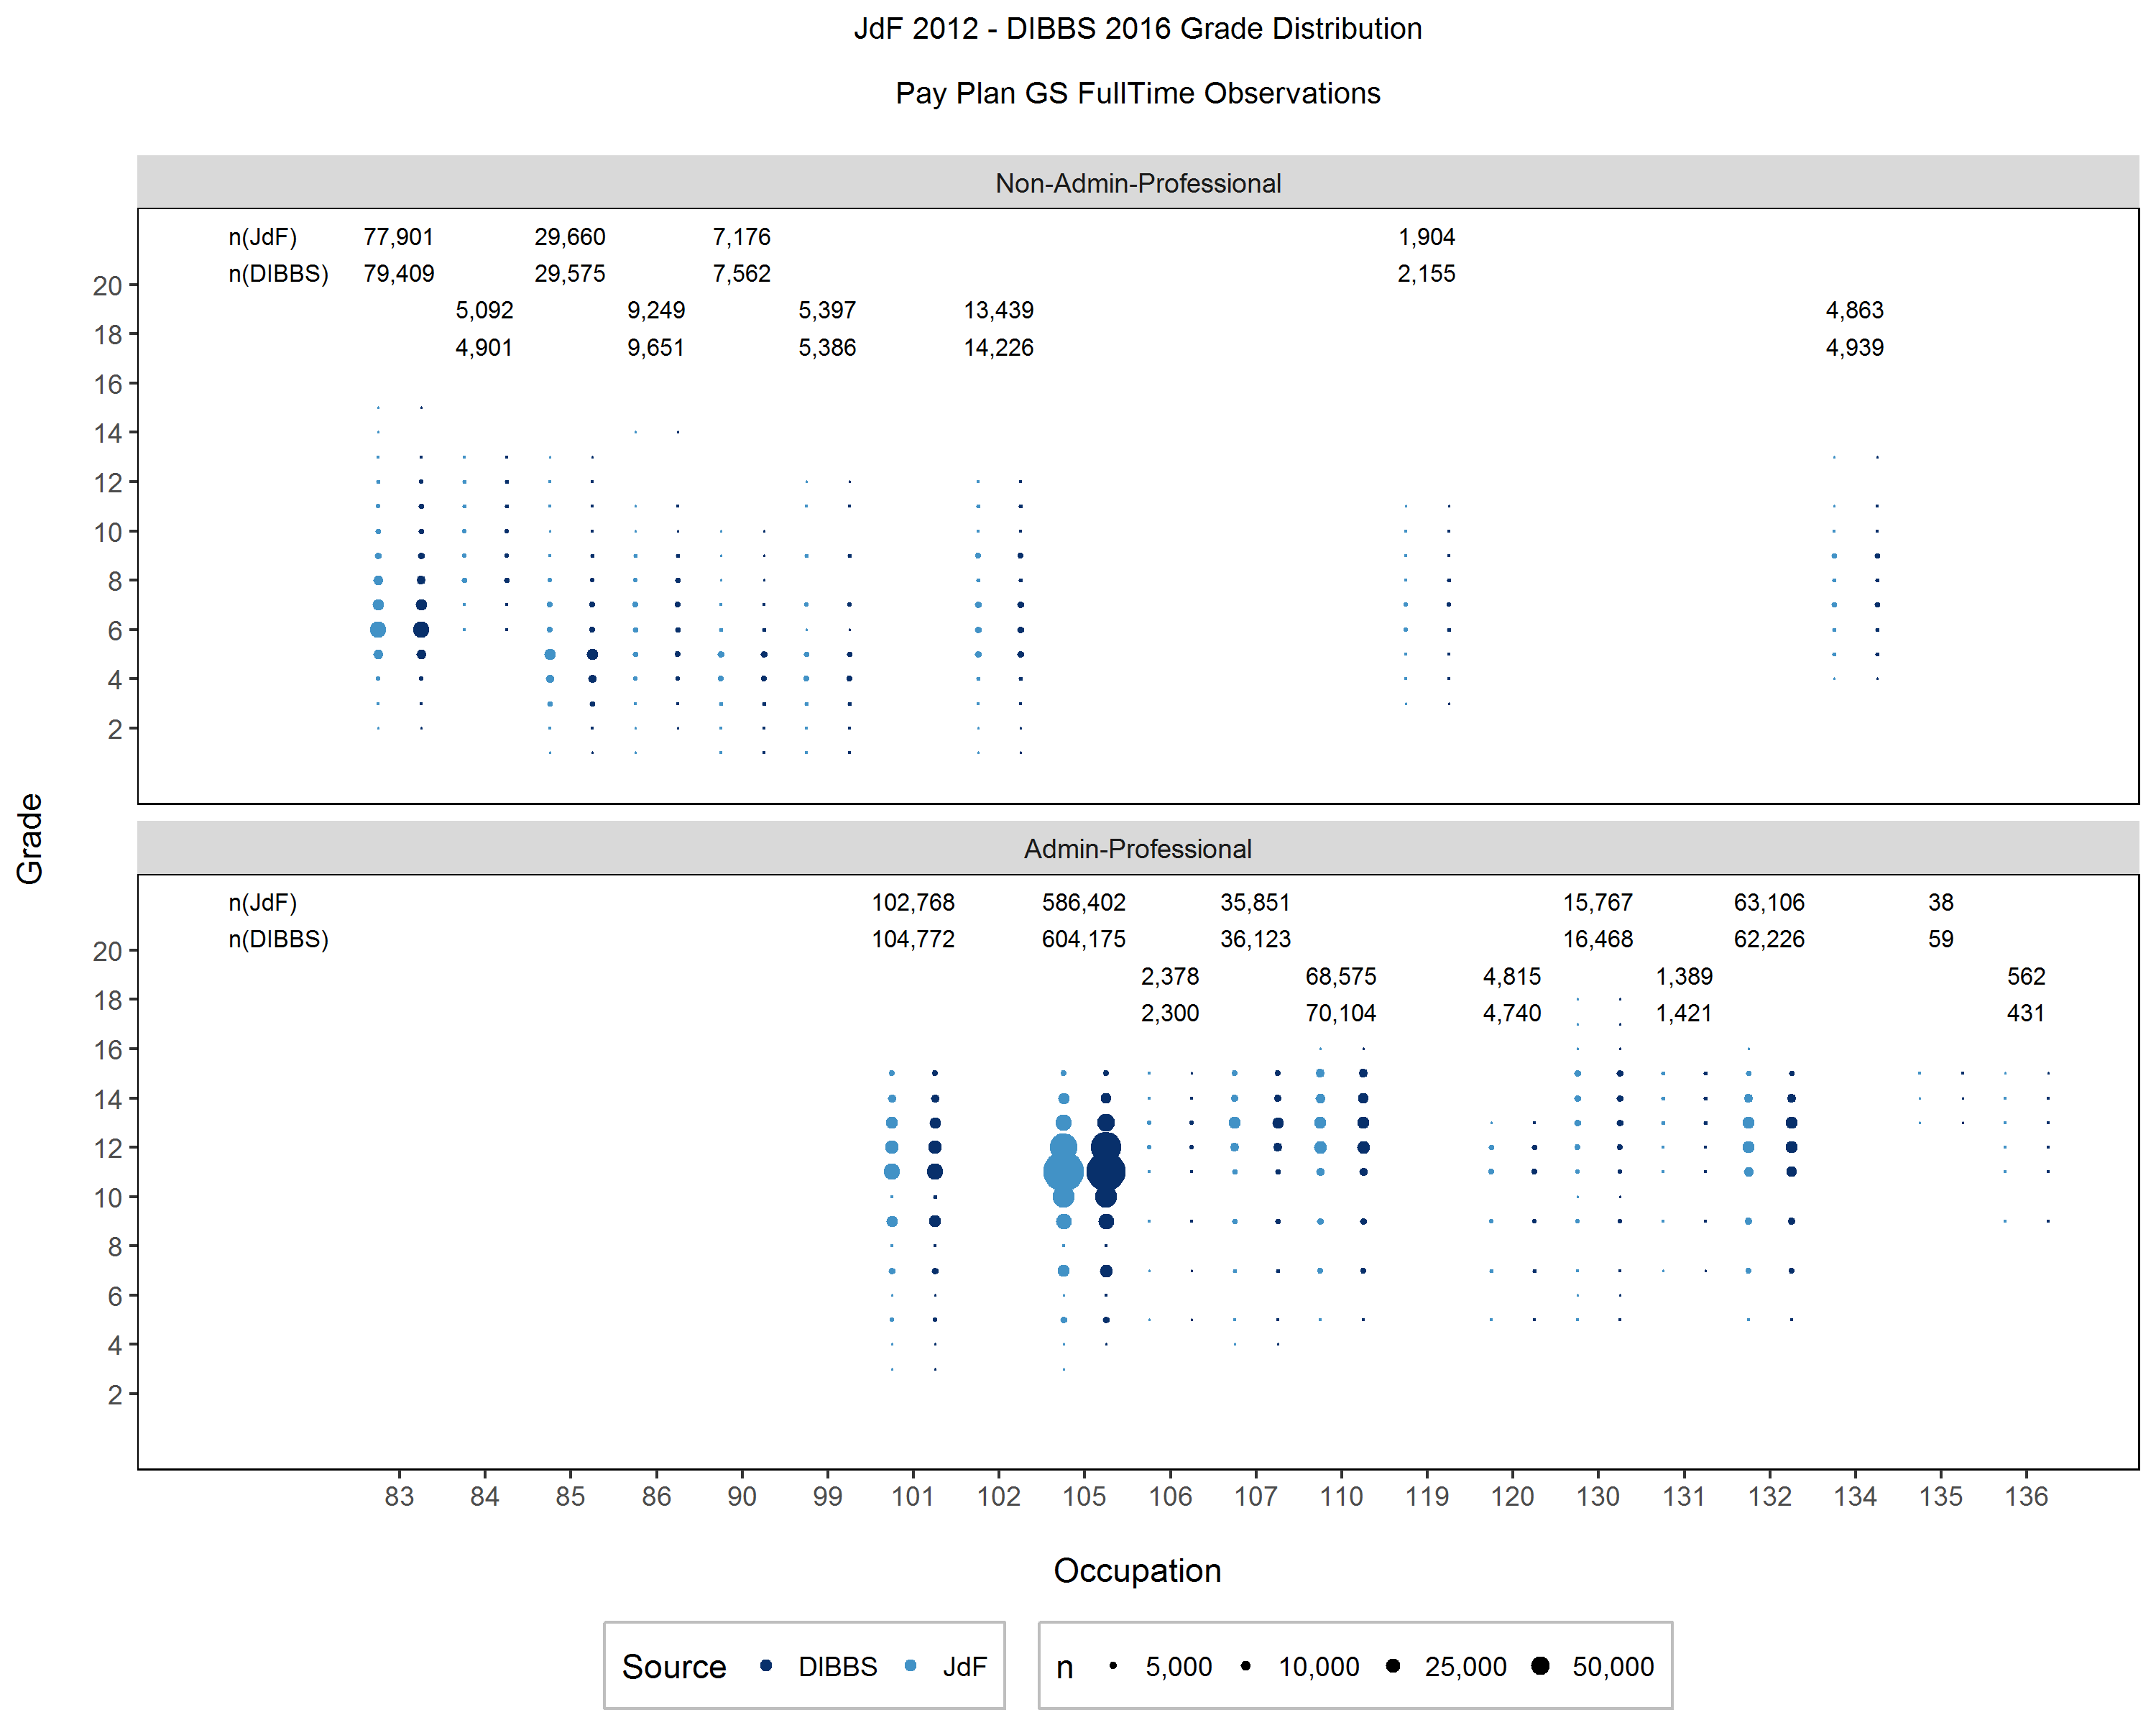
\includegraphics[width=6in, trim={0 200px 0 165px}, clip]{JdFDIBBSGSFullTimeGradeAdminProfessionalOccupation21.png}
        \caption{Occupations 0083 through 0136}
        \vspace{10pt}
    \end{subfigure}
    \caption{Distribution of grade by occupation.  Occupational categories Admin/Professional vs. non Admin/Professional.  Authentic on left, synthetic on right.  Dot size small (n$<$5,000) to large (n$>$250,000).  Occupations on x-axis.}
    \label{figure:JdFDIBBSGSFullTimeGradeAdminProfessionalOccupation}
\end{figure}

\clearpage

\begin{figure}[]
    \centering
    \begin{subfigure}{1\textwidth}
        \centering
        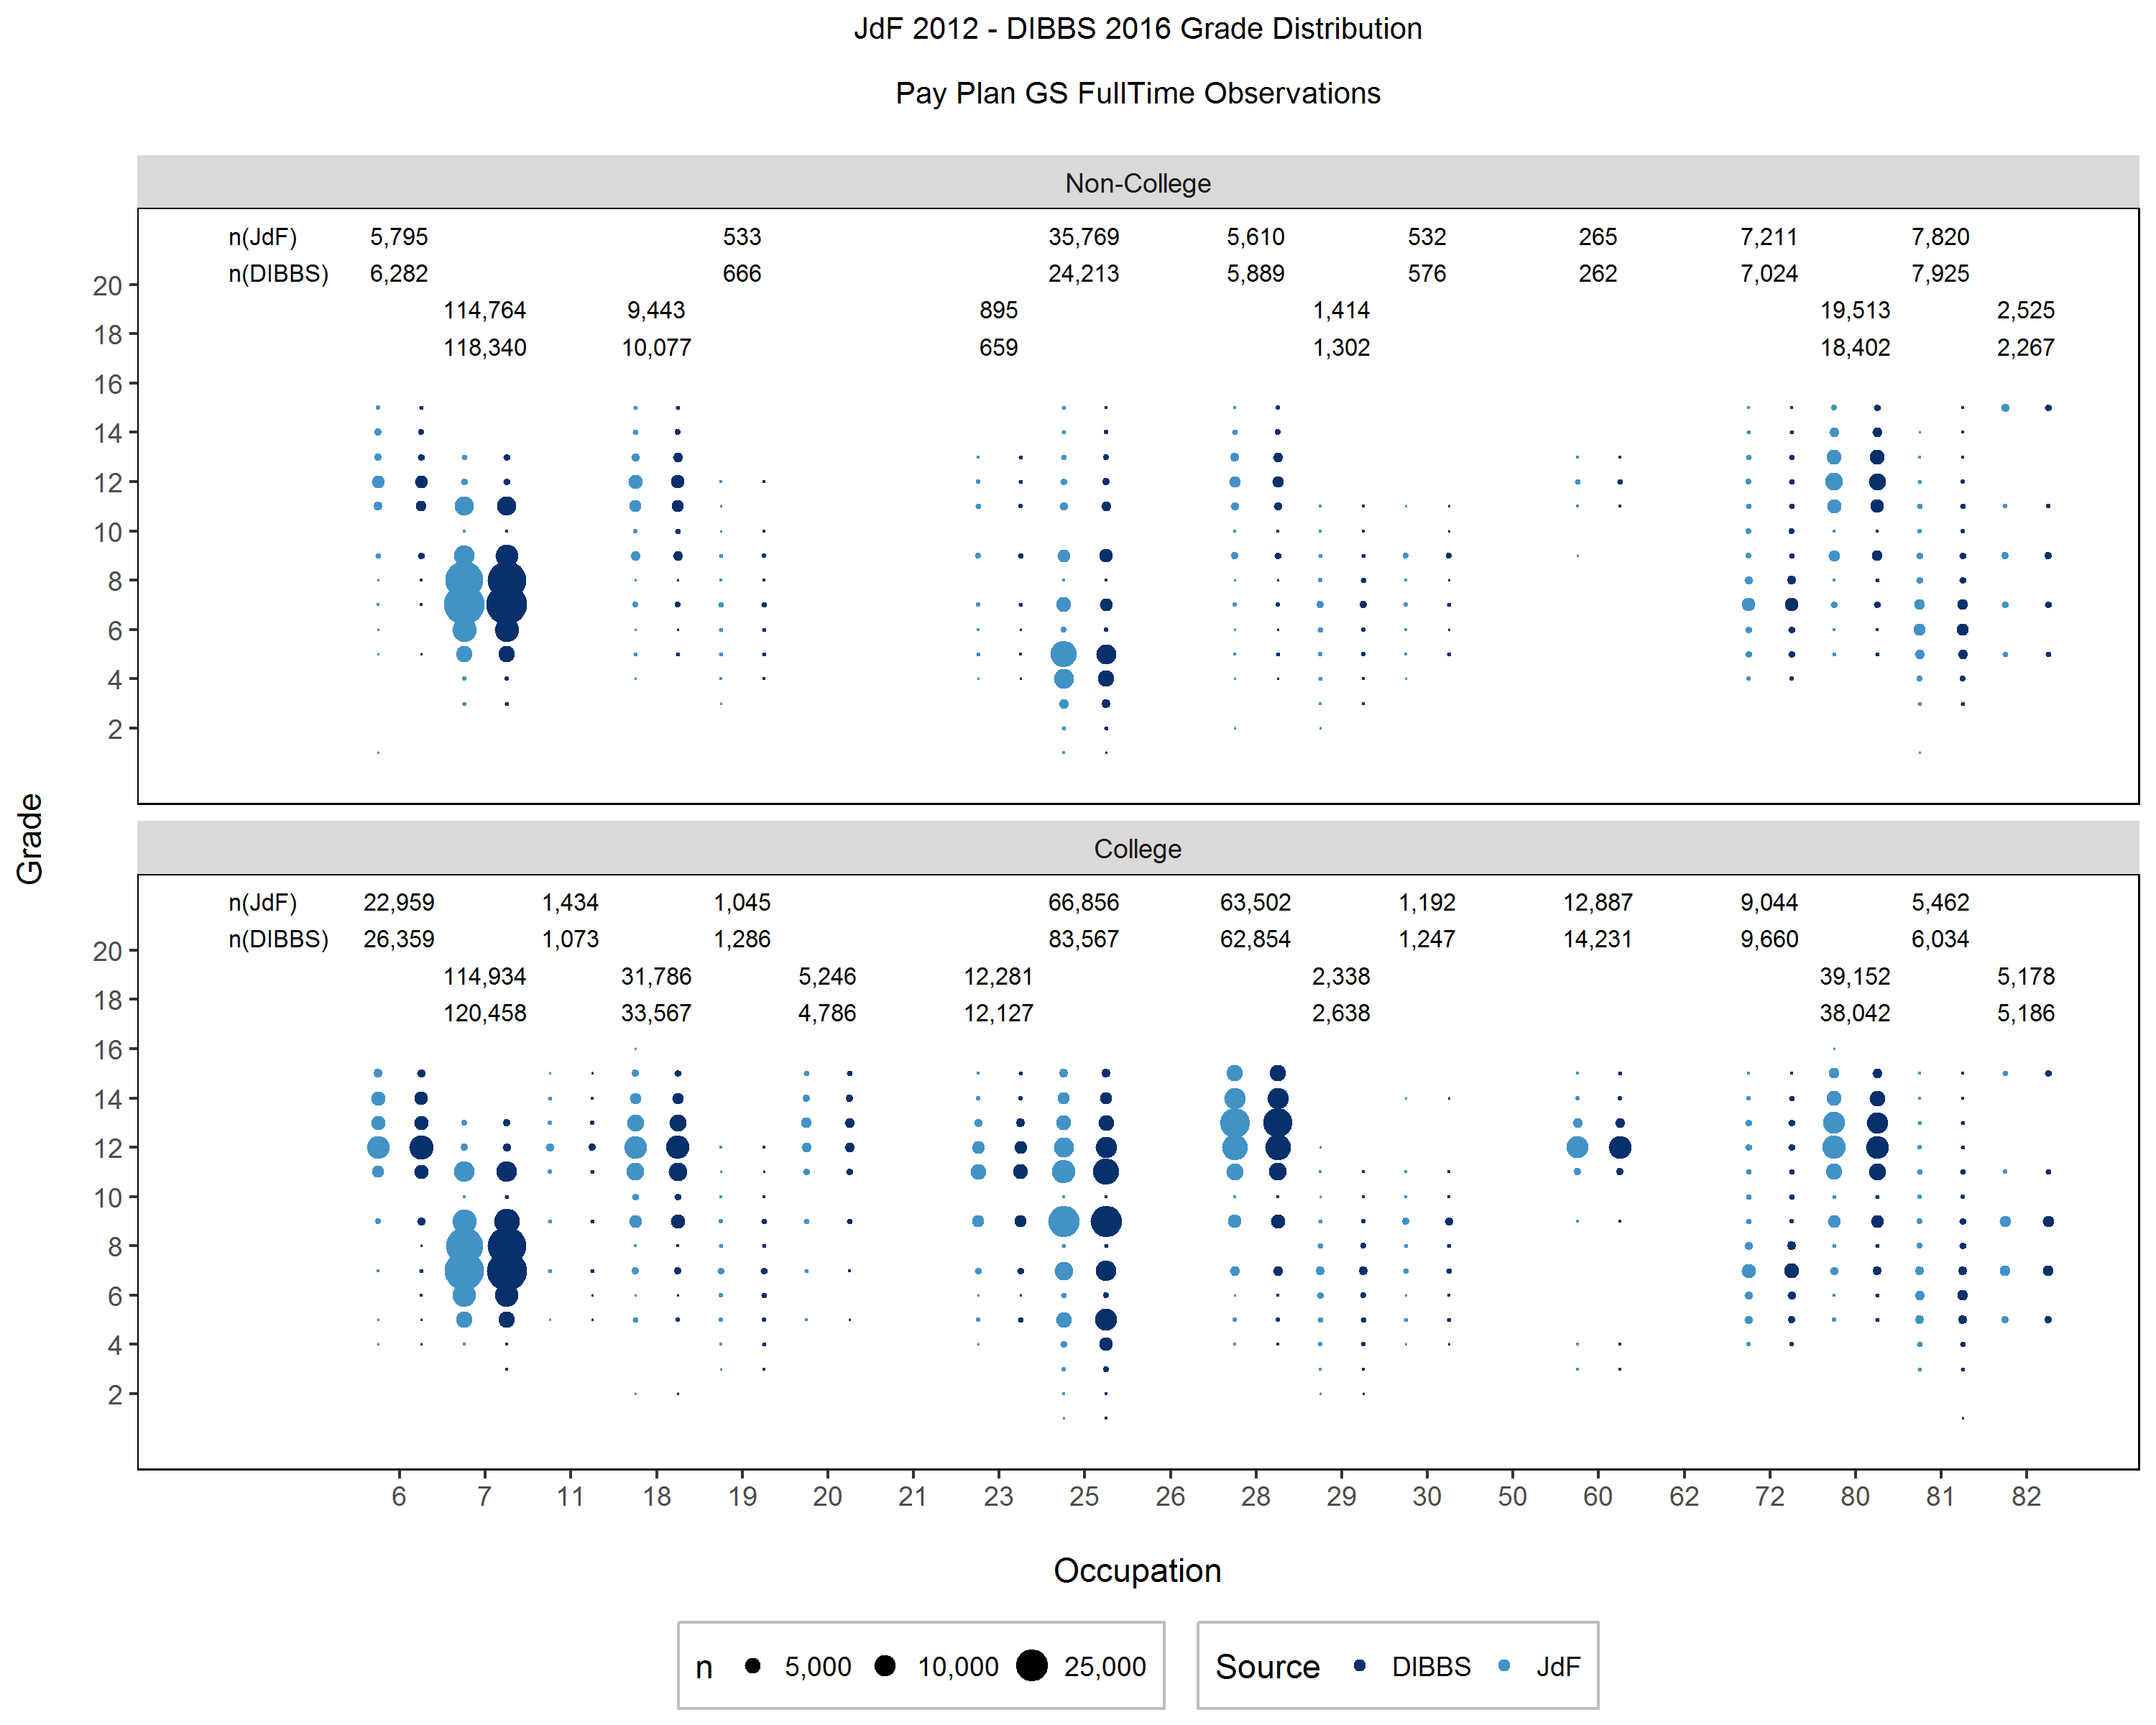
\includegraphics[width=6in, trim={0 200px 0 165px}, clip]{JdFDIBBSGSFullTimeGradeCollegeOccupation1.png}
        \caption{Occupations 0006 through 0082}
        \vspace{20pt}
    \end{subfigure}
    \begin{subfigure}{1\textwidth}
        \centering
        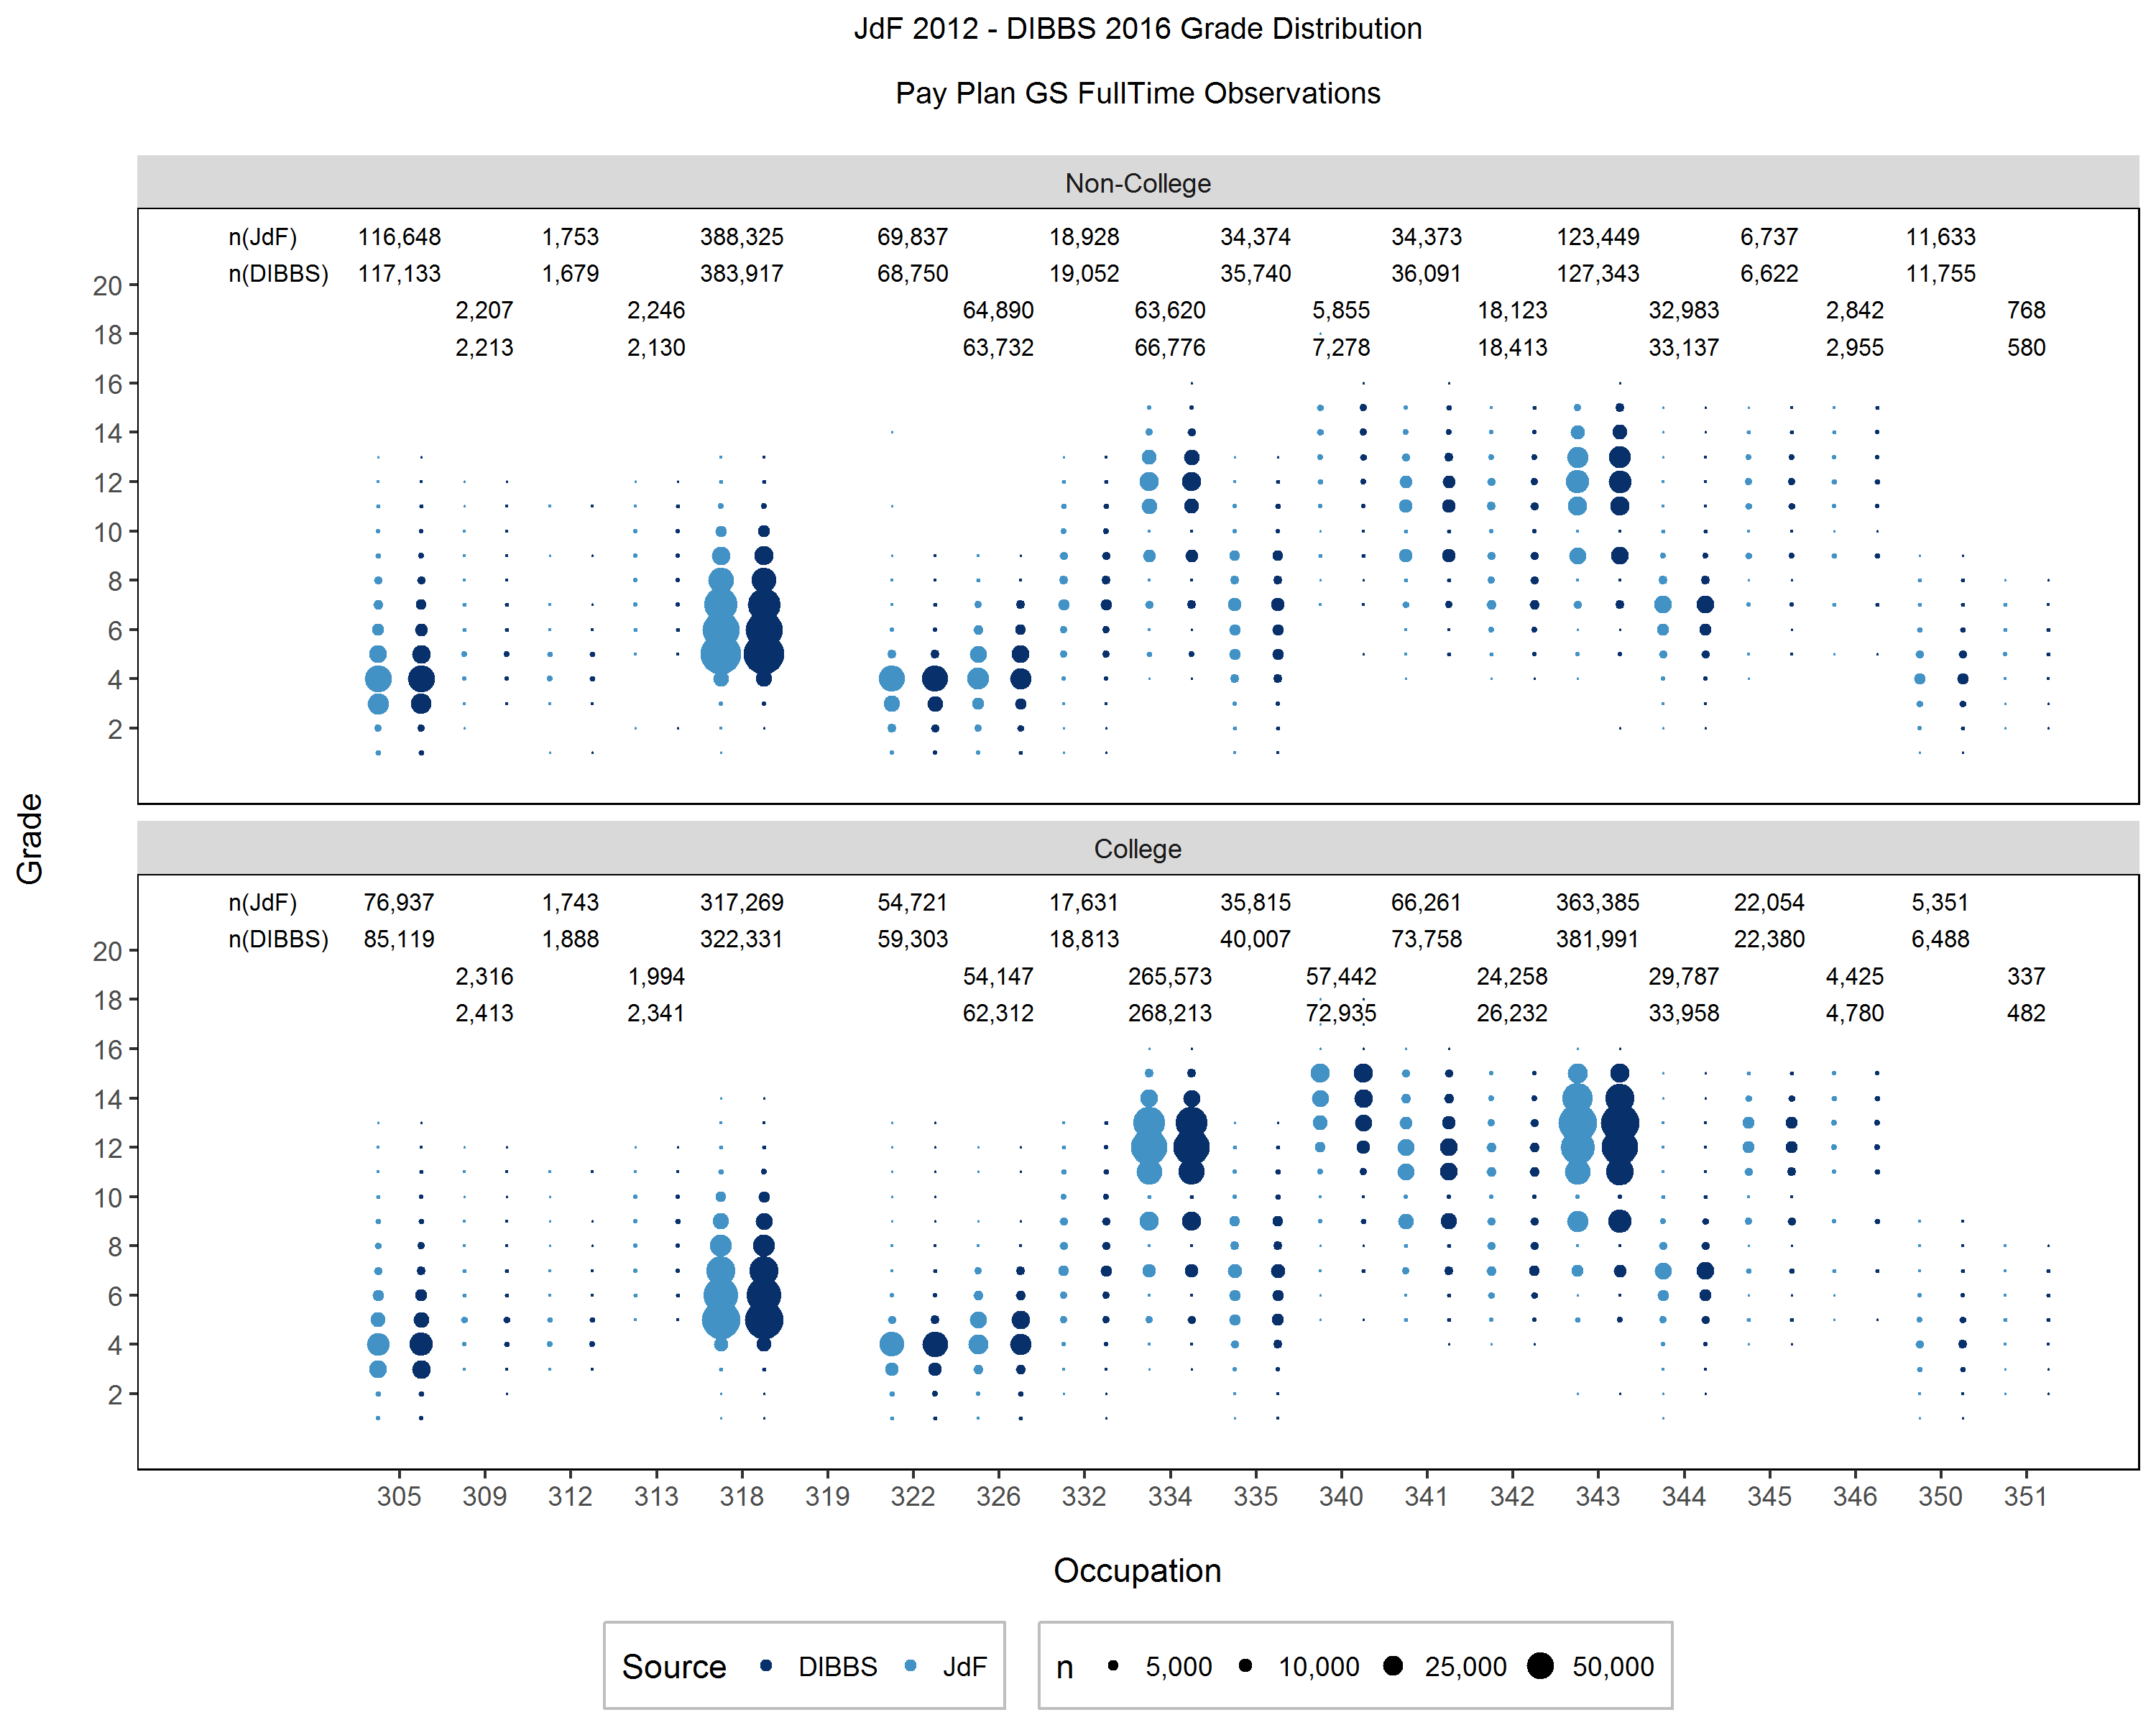
\includegraphics[width=6in, trim={0 200px 0 165px}, clip]{JdFDIBBSGSFullTimeGradeCollegeOccupation81.png}
        \caption{Occupations 0305 through 0351}
        \vspace{10pt}
    \end{subfigure}
    \caption{Distribution of grade by occupation.  College education vs. non-college.  Authentic on left, synthetic on right.  Dot size small (n$<$5,000) to large (n$>$250,000).  Occupations on x-axis.}
    \label{figure:JdFDIBBSGSFullTimeGradeCollegeOccupation}
\end{figure}

\clearpage

\begin{figure}[]
    \centering
    \begin{subfigure}{1\textwidth}
        \centering
        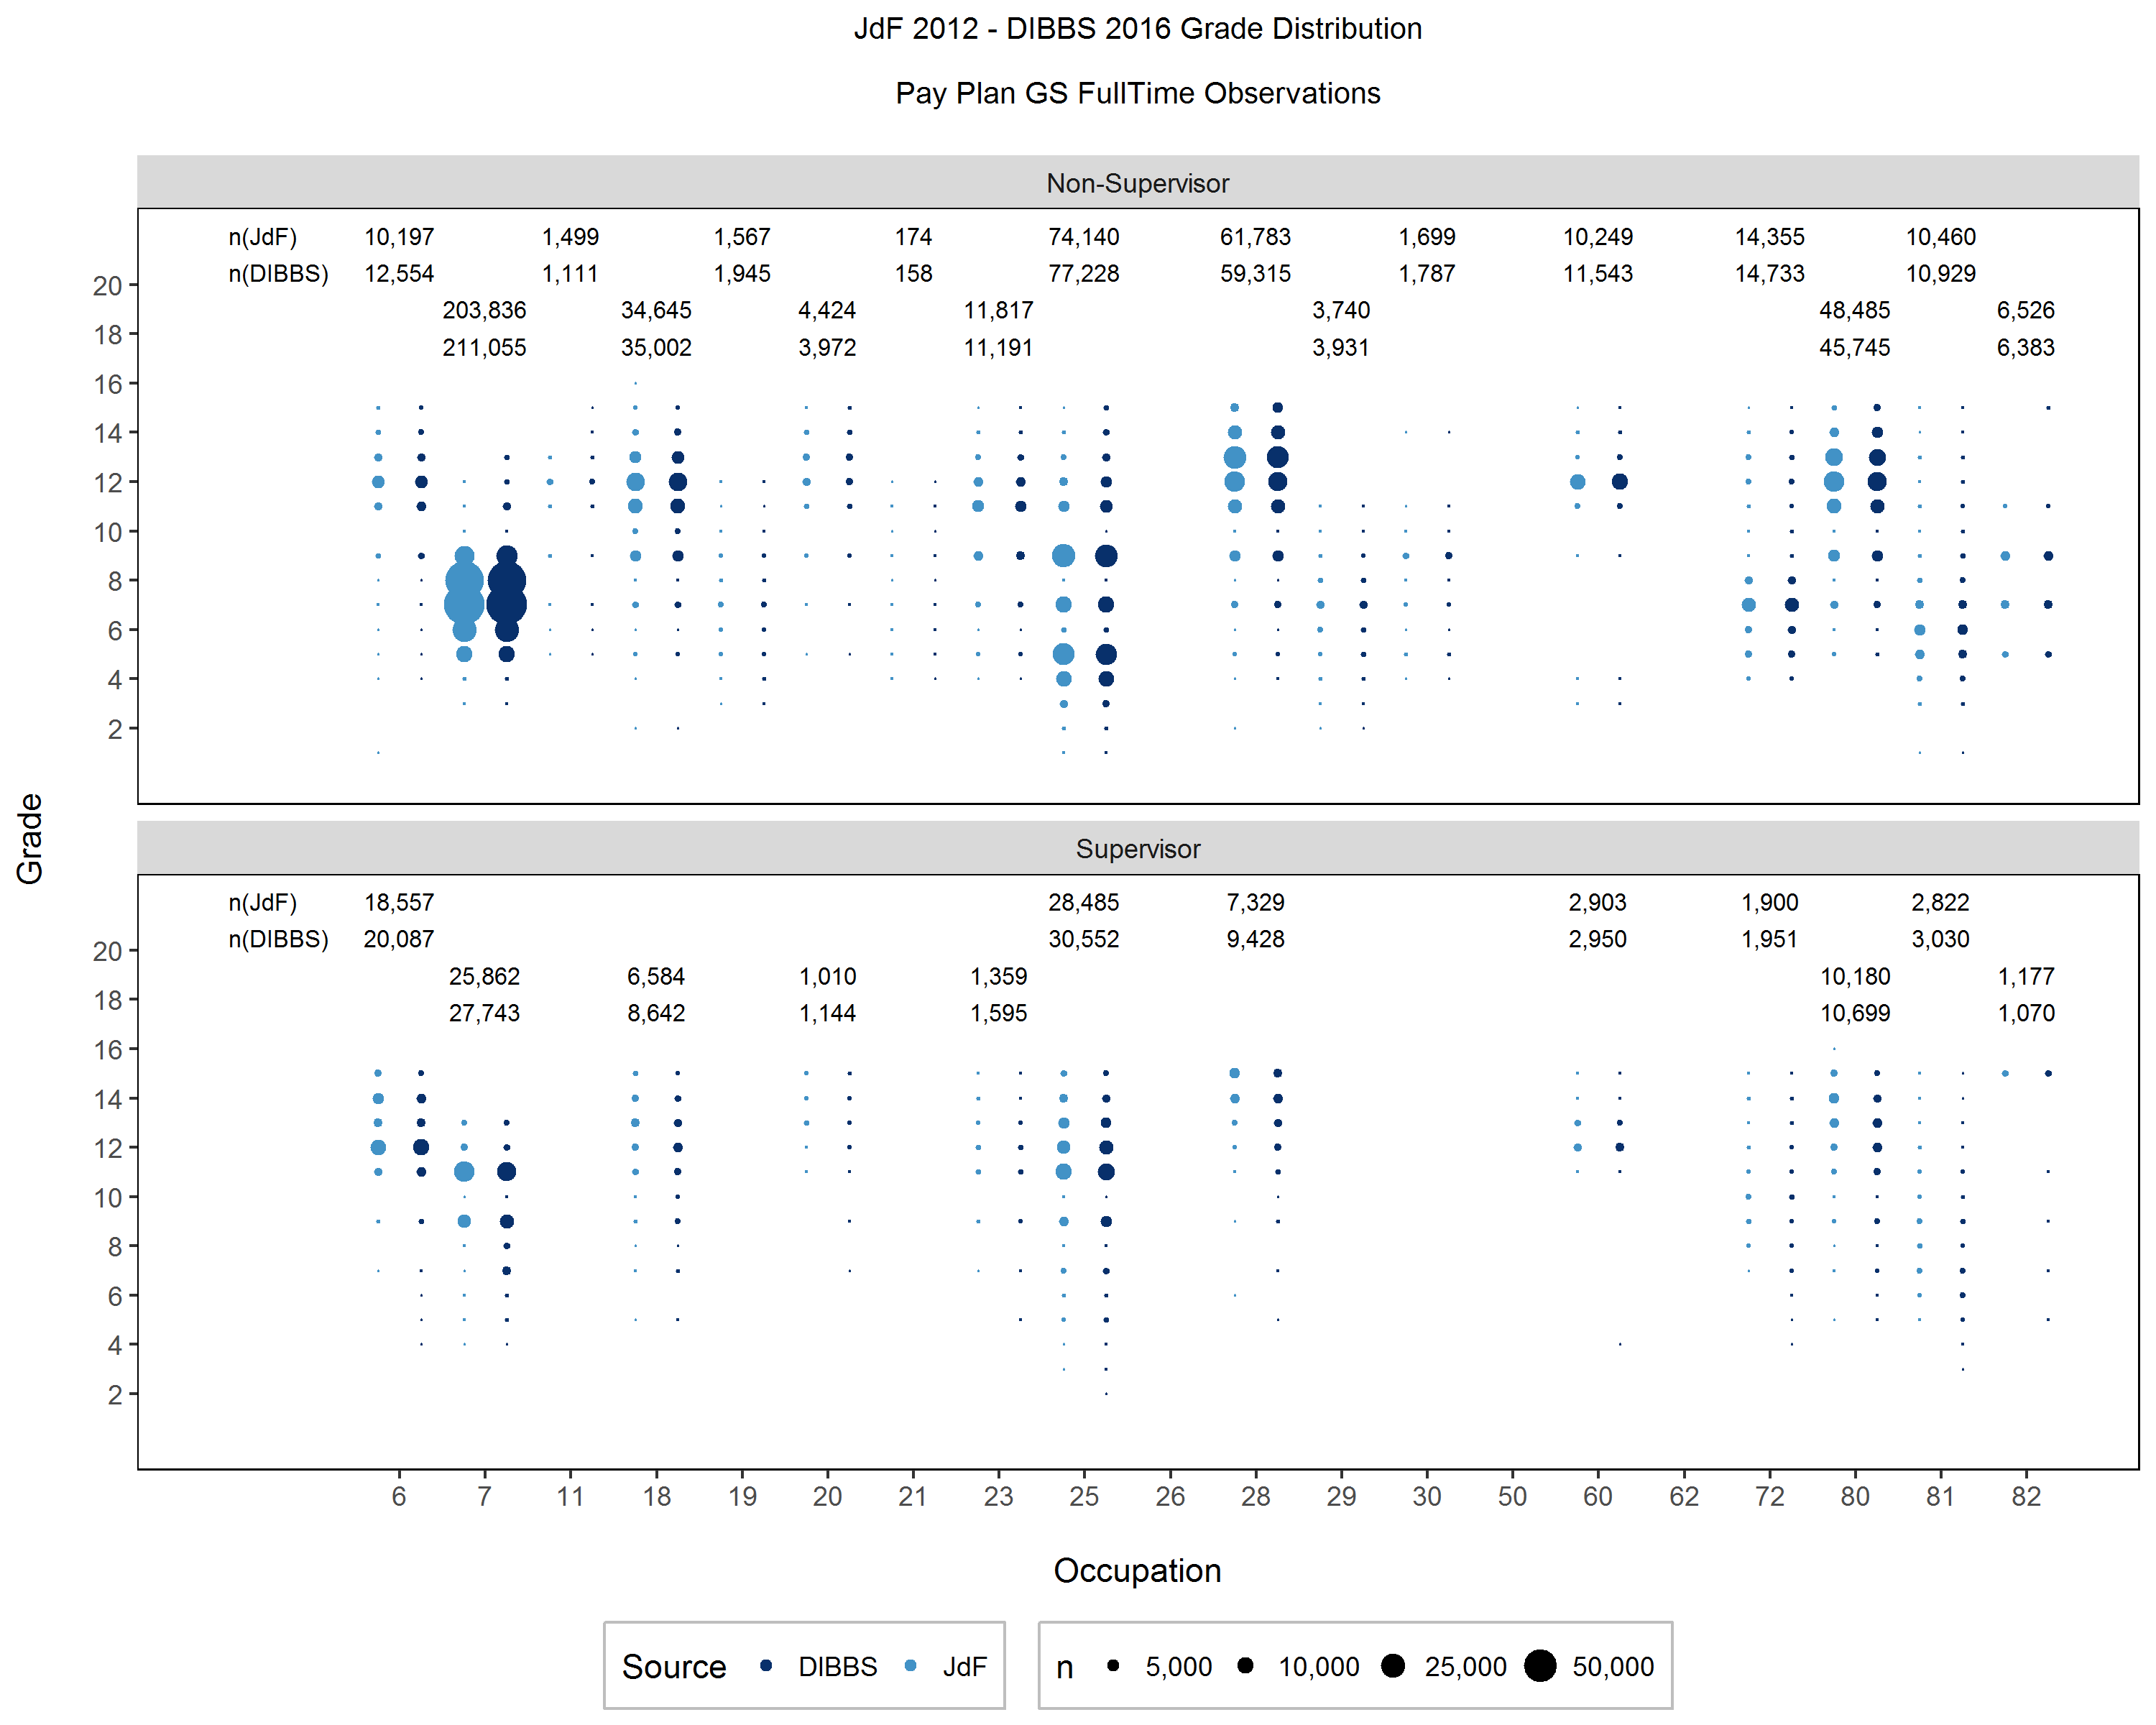
\includegraphics[width=6in, trim={0 200px 0 165px}, clip]{JdFDIBBSGSFullTimeGradeSupervisoryStatusOccupation1.png}
        \caption{Occupations 0006 through 0082}
        \vspace{20pt}
    \end{subfigure}
    \begin{subfigure}{1\textwidth}
        \centering
        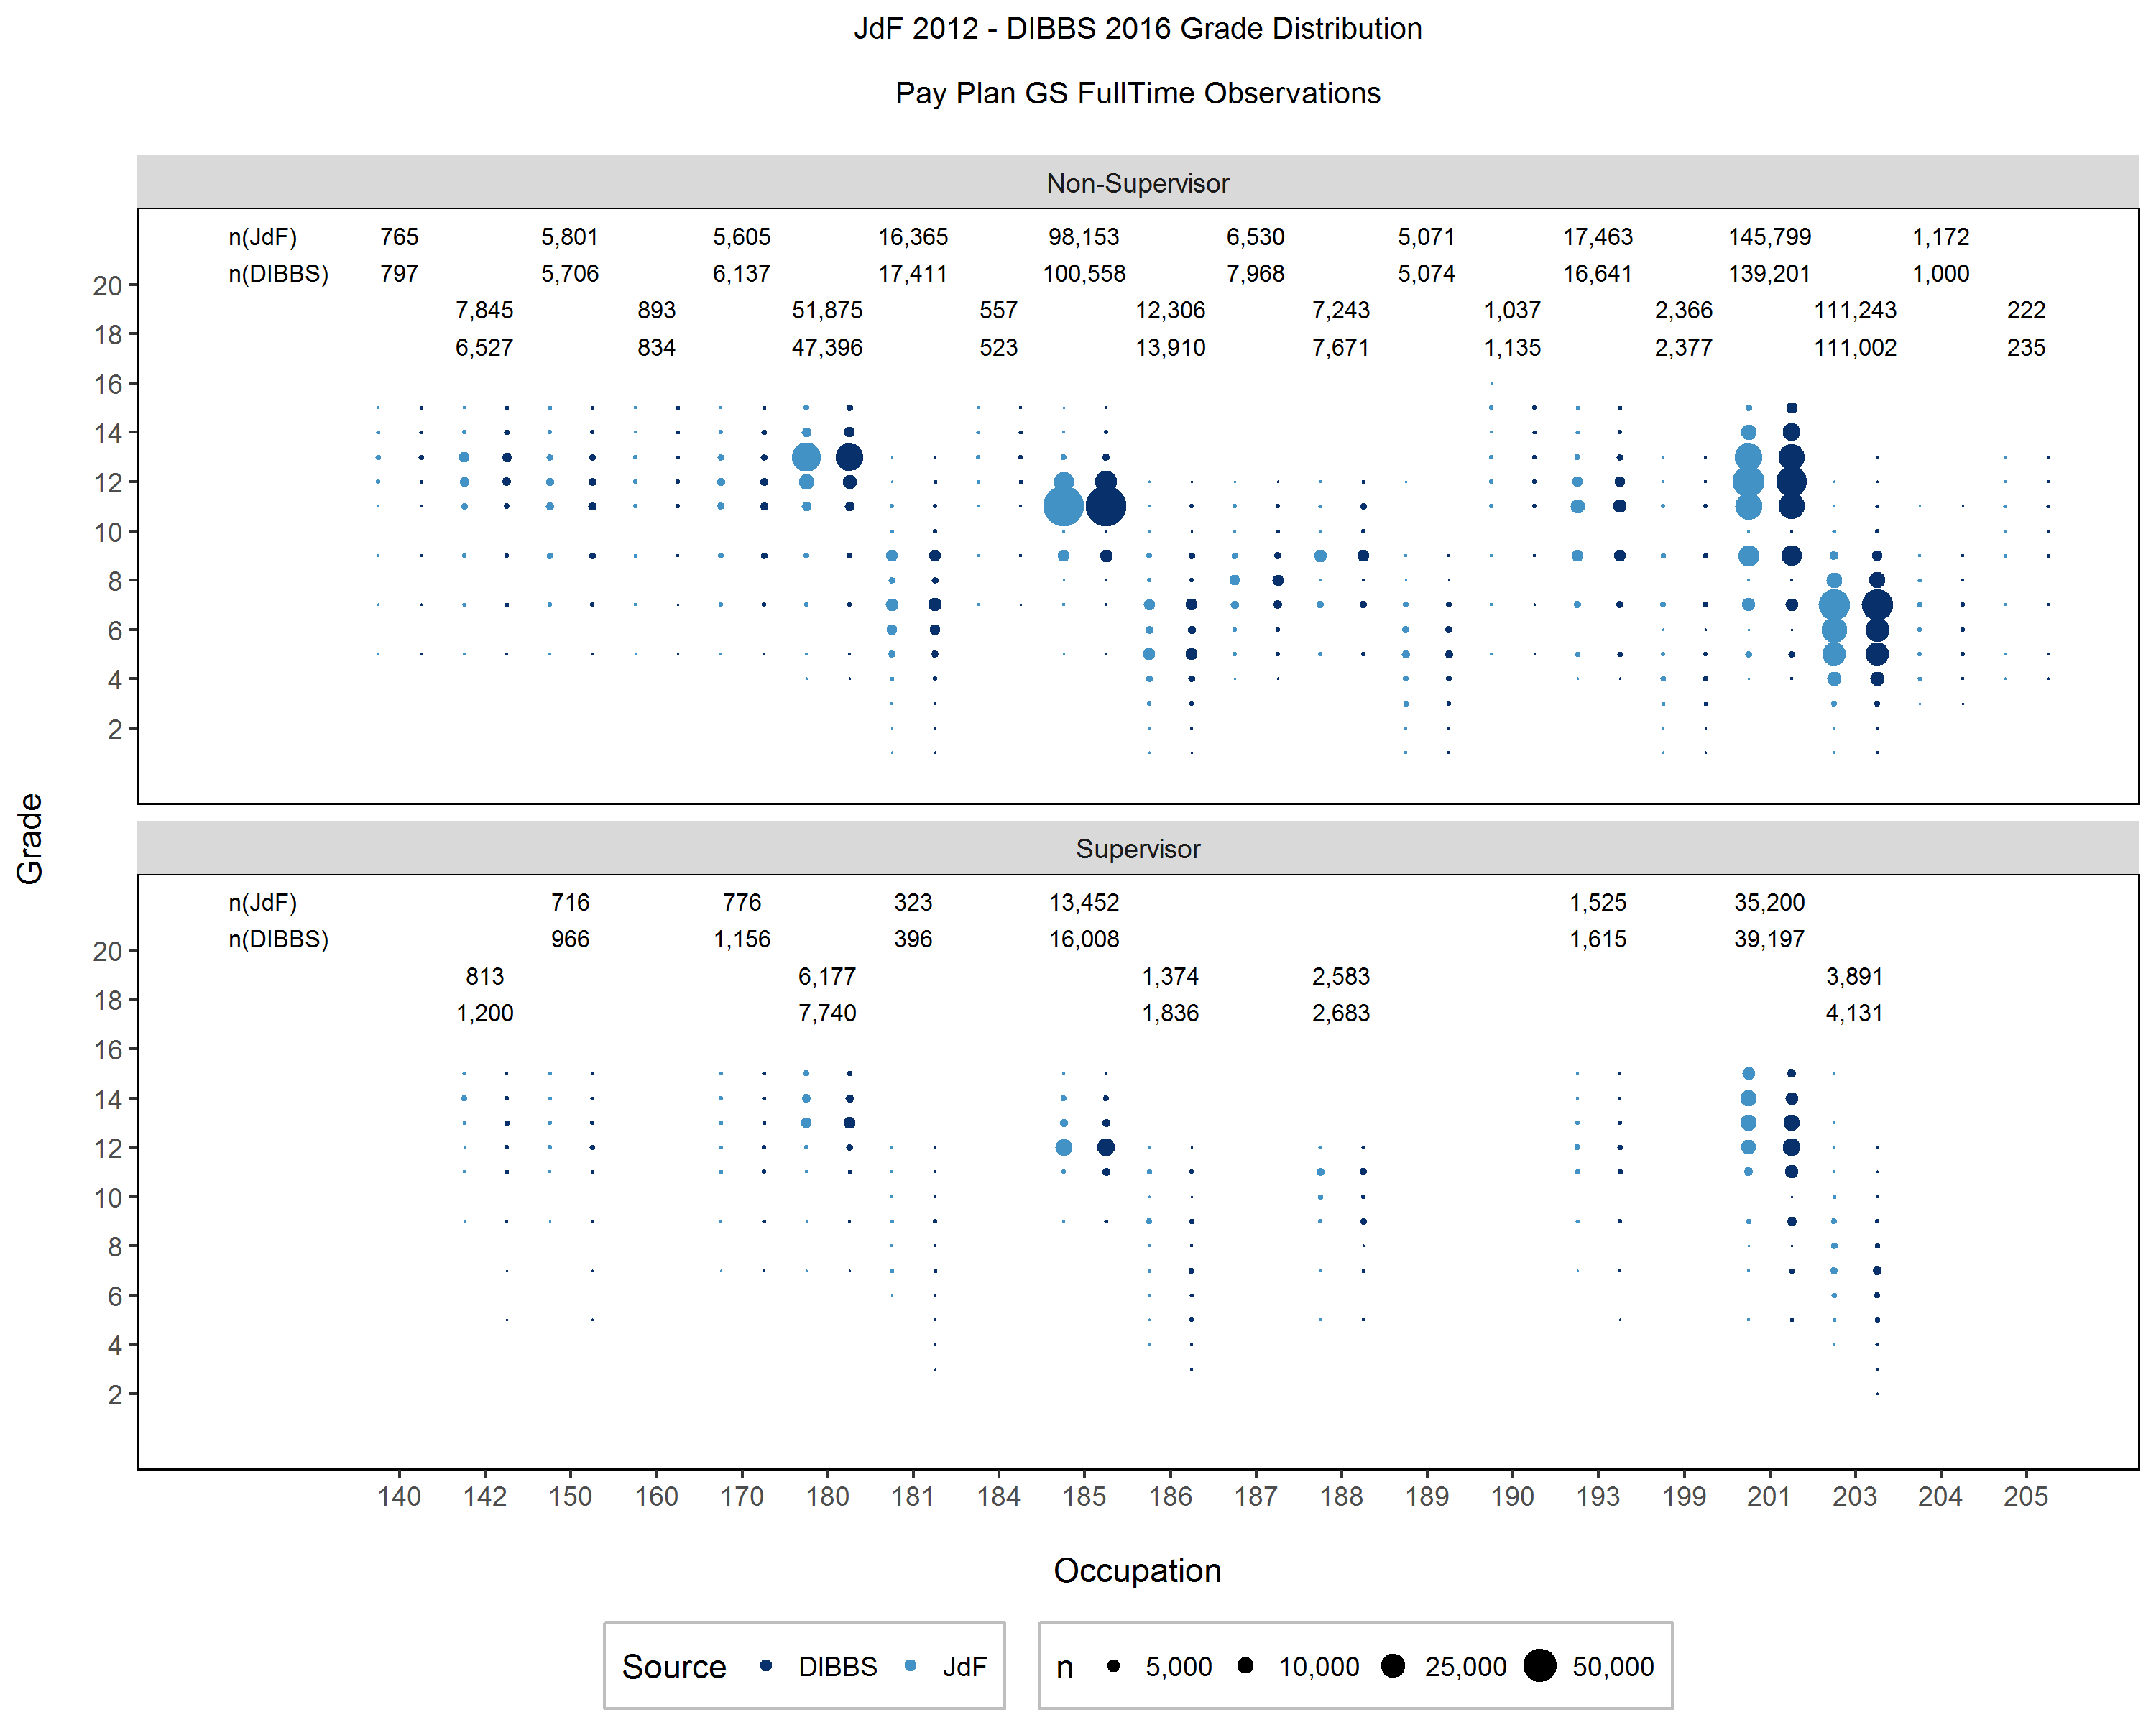
\includegraphics[width=6in, trim={0 200px 0 165px}, clip]{JdFDIBBSGSFullTimeGradeSupervisoryStatusOccupation41.png}
        \caption{Occupations 0140 through 0205}
        \vspace{10pt}
    \end{subfigure}
    \caption{Distribution of grade by agency and supervisor status.  Authentic on left, synthetic on right.  Dot size small (n$<$5,000) to large (n$>$250,000).  Occupations on x-axis.}
    \label{figure:JdFDIBBSGSFullTimeGradeSupervisoryStatusOccupation}
\end{figure}

\clearpage

\begin{figure}[]
    \centering
    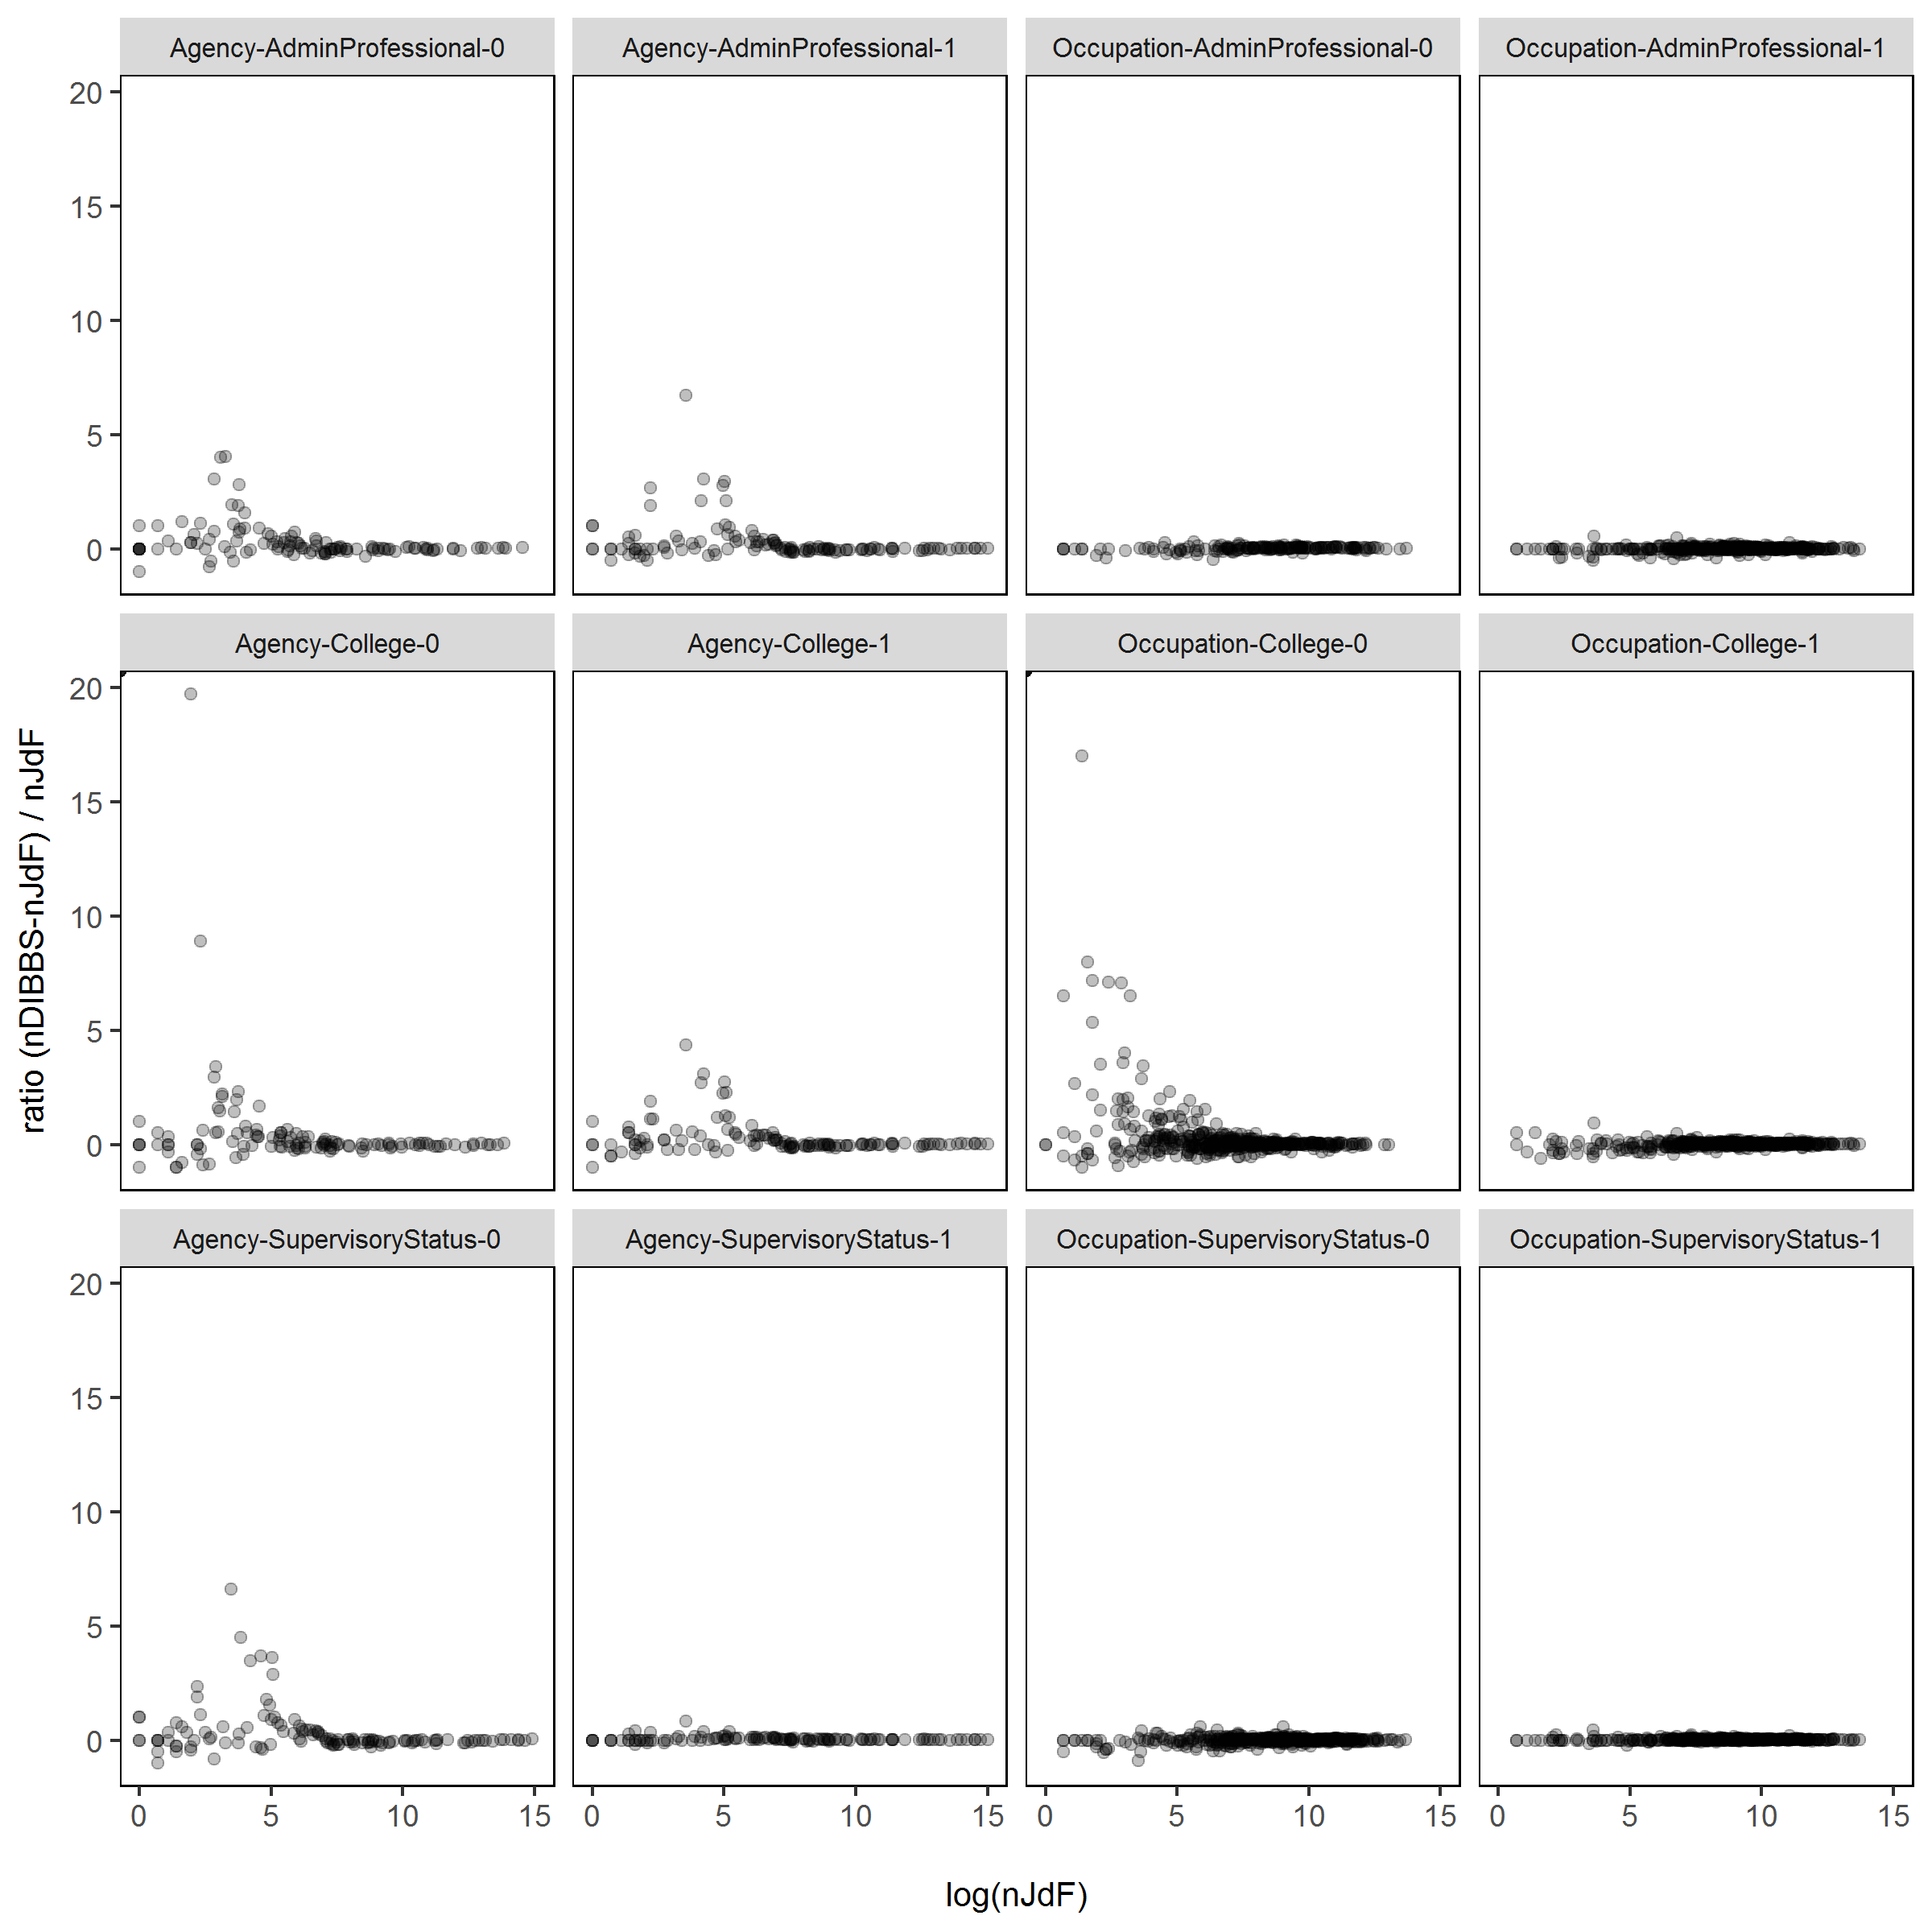
\includegraphics[width=6in]{nRatioGrade.png}
    \caption{Ratio of difference in synthetic and authentic observation count to authentic observation count.  Suffix of 0 indicates non-Admin, non-College, or non-Supervisor, suffix of 1 indicates Admin, College, or Supervisor.  Log x-axis scale.  Differences tend to be positive (synthetic $>$ authentic).  General decrease in error proportion with increase in n.}
    \label{figure:nRatioGrade}
\end{figure}

\clearpage

\section{Distribution of Basic Pay}

Basic pay is an important dependent study variable and the distribution of pay values in the authentic data must be maintained in the synthetic data.\footnote{Basic pay is determined by pay plan, grade, and step rate and does not include adjustments such as for locale.} \footnote{Due to inflation, the value of wages earned is variable, typically decreasing by year.  To compensate for this, and to make inter-year values comparable, pay values throughout the entire document are adjusted to 2011 dollars using annual consumer price indices.}

\subsection{Distribution of Basic Pay by Agency}

Figure \ref{figure:JdFDIBBSBasicPayDistribution} plots the distribution of basic pay for the top eight frequency agencies (first two positions):  Department of Agriculture (AG), Department of Justice (DJ), Department of Health and Human Services (HE), Department of Homeland Security (HS), Department of Interior (IN), Department of Transportation (TD), Department of Treasury (TR), and the Department of Veterans Affairs (VA).  These agencies account for approximately 85\% of observations.  Synthetic distribution represented by dashed line, authentic distribution by solid line.  ``n(D)" indicates synthetic data observation frequency, ``n(J)" indicates authentic data observation count.\\

Observations:  Although each data set is represented in each graph, a single striped-appearing line is visible, due to identical frequency proportions at each pay level.  Local increases, decreases, and trends in authentic distribution are accurately represented in the synthetic data.\\

\begin{figure}[h]
    \centering
    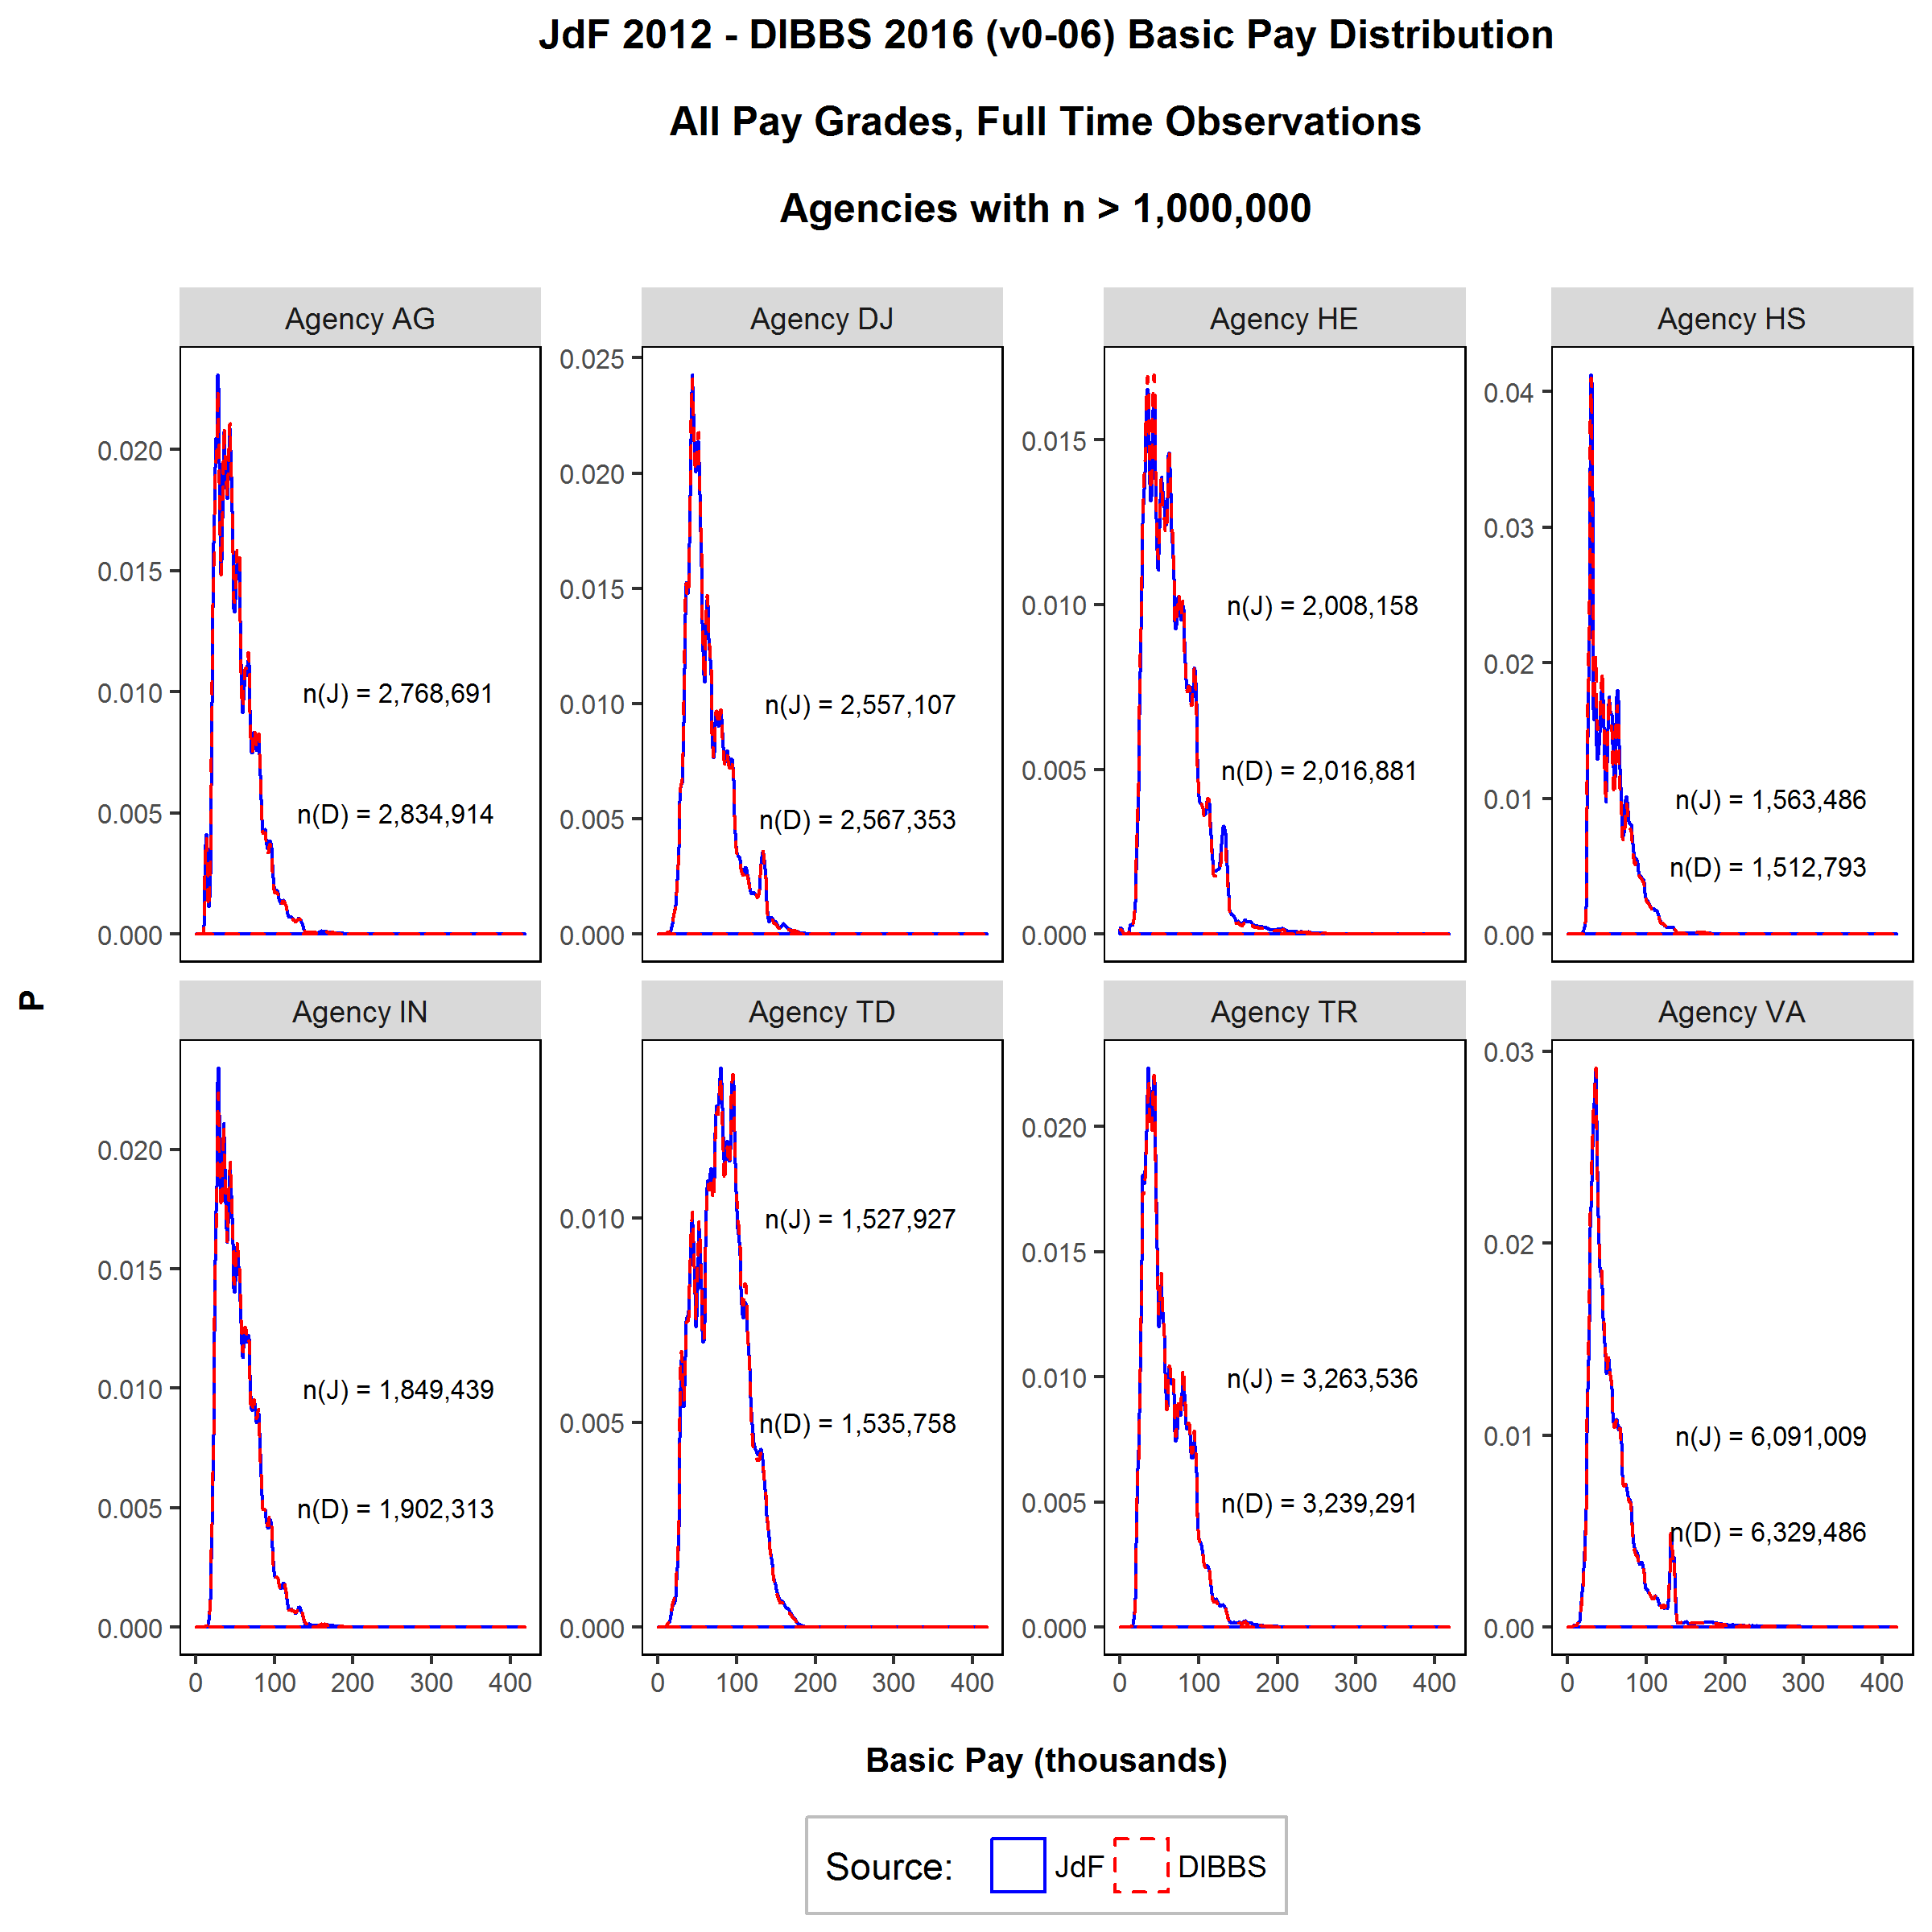
\includegraphics[width=6in, trim={0 0.8in 0 1.2in}, clip]{JdFDIBBSBasicPayDistribution.png}
    \caption{Basic pay marginal distribution for top eight agencies.  Dashed line for synthetic data, solid line for authentic.  Basic pay  (in thousands) on x-axis.}
    \label{figure:JdFDIBBSBasicPayDistribution}
\end{figure}

\clearpage

\subsection{Distribution of Basic Pay by Professional, Supervisory, College Education, and Work Schedule Category}

Professional classification, supervisory status, and college education are important independent variables in human capital research.  Figures \ref{figure:JdFDIBBSBasicPayCDFAG} through \ref{figure:JdFDIBBSBasicPayCDFVA} plot, for the top eight frequency agencies, the distribution of basic pay by these independent variables and work schedule code.  One column for each professional, supervisory, college combination (column code position one equals ``P" if occupational category is administrative or professional, position two equals ``S" if supervisory status is enabled, position three equals ``C" if education level at or above college).  One row for each work schedule code [significant codes are full time (F), full time seasonal (G), intermittent (I), intermittent seasonal (J), and part time (P)].  Synthetic distribution indicated by dashed line, authentic distribution by solid line.  ``n(D)" indicates synthetic data observation frequency, ``n(J)" indicates authentic data observation count.\\

Observations:  There exists near identical distribution for high frequency combinations, as indicated by striped, single line appearance due to overlay of synthetic on authentic lines.  Slight differences in distribution are observed for small frequency combinations.\\

\begin{figure}[h]
    \centering
    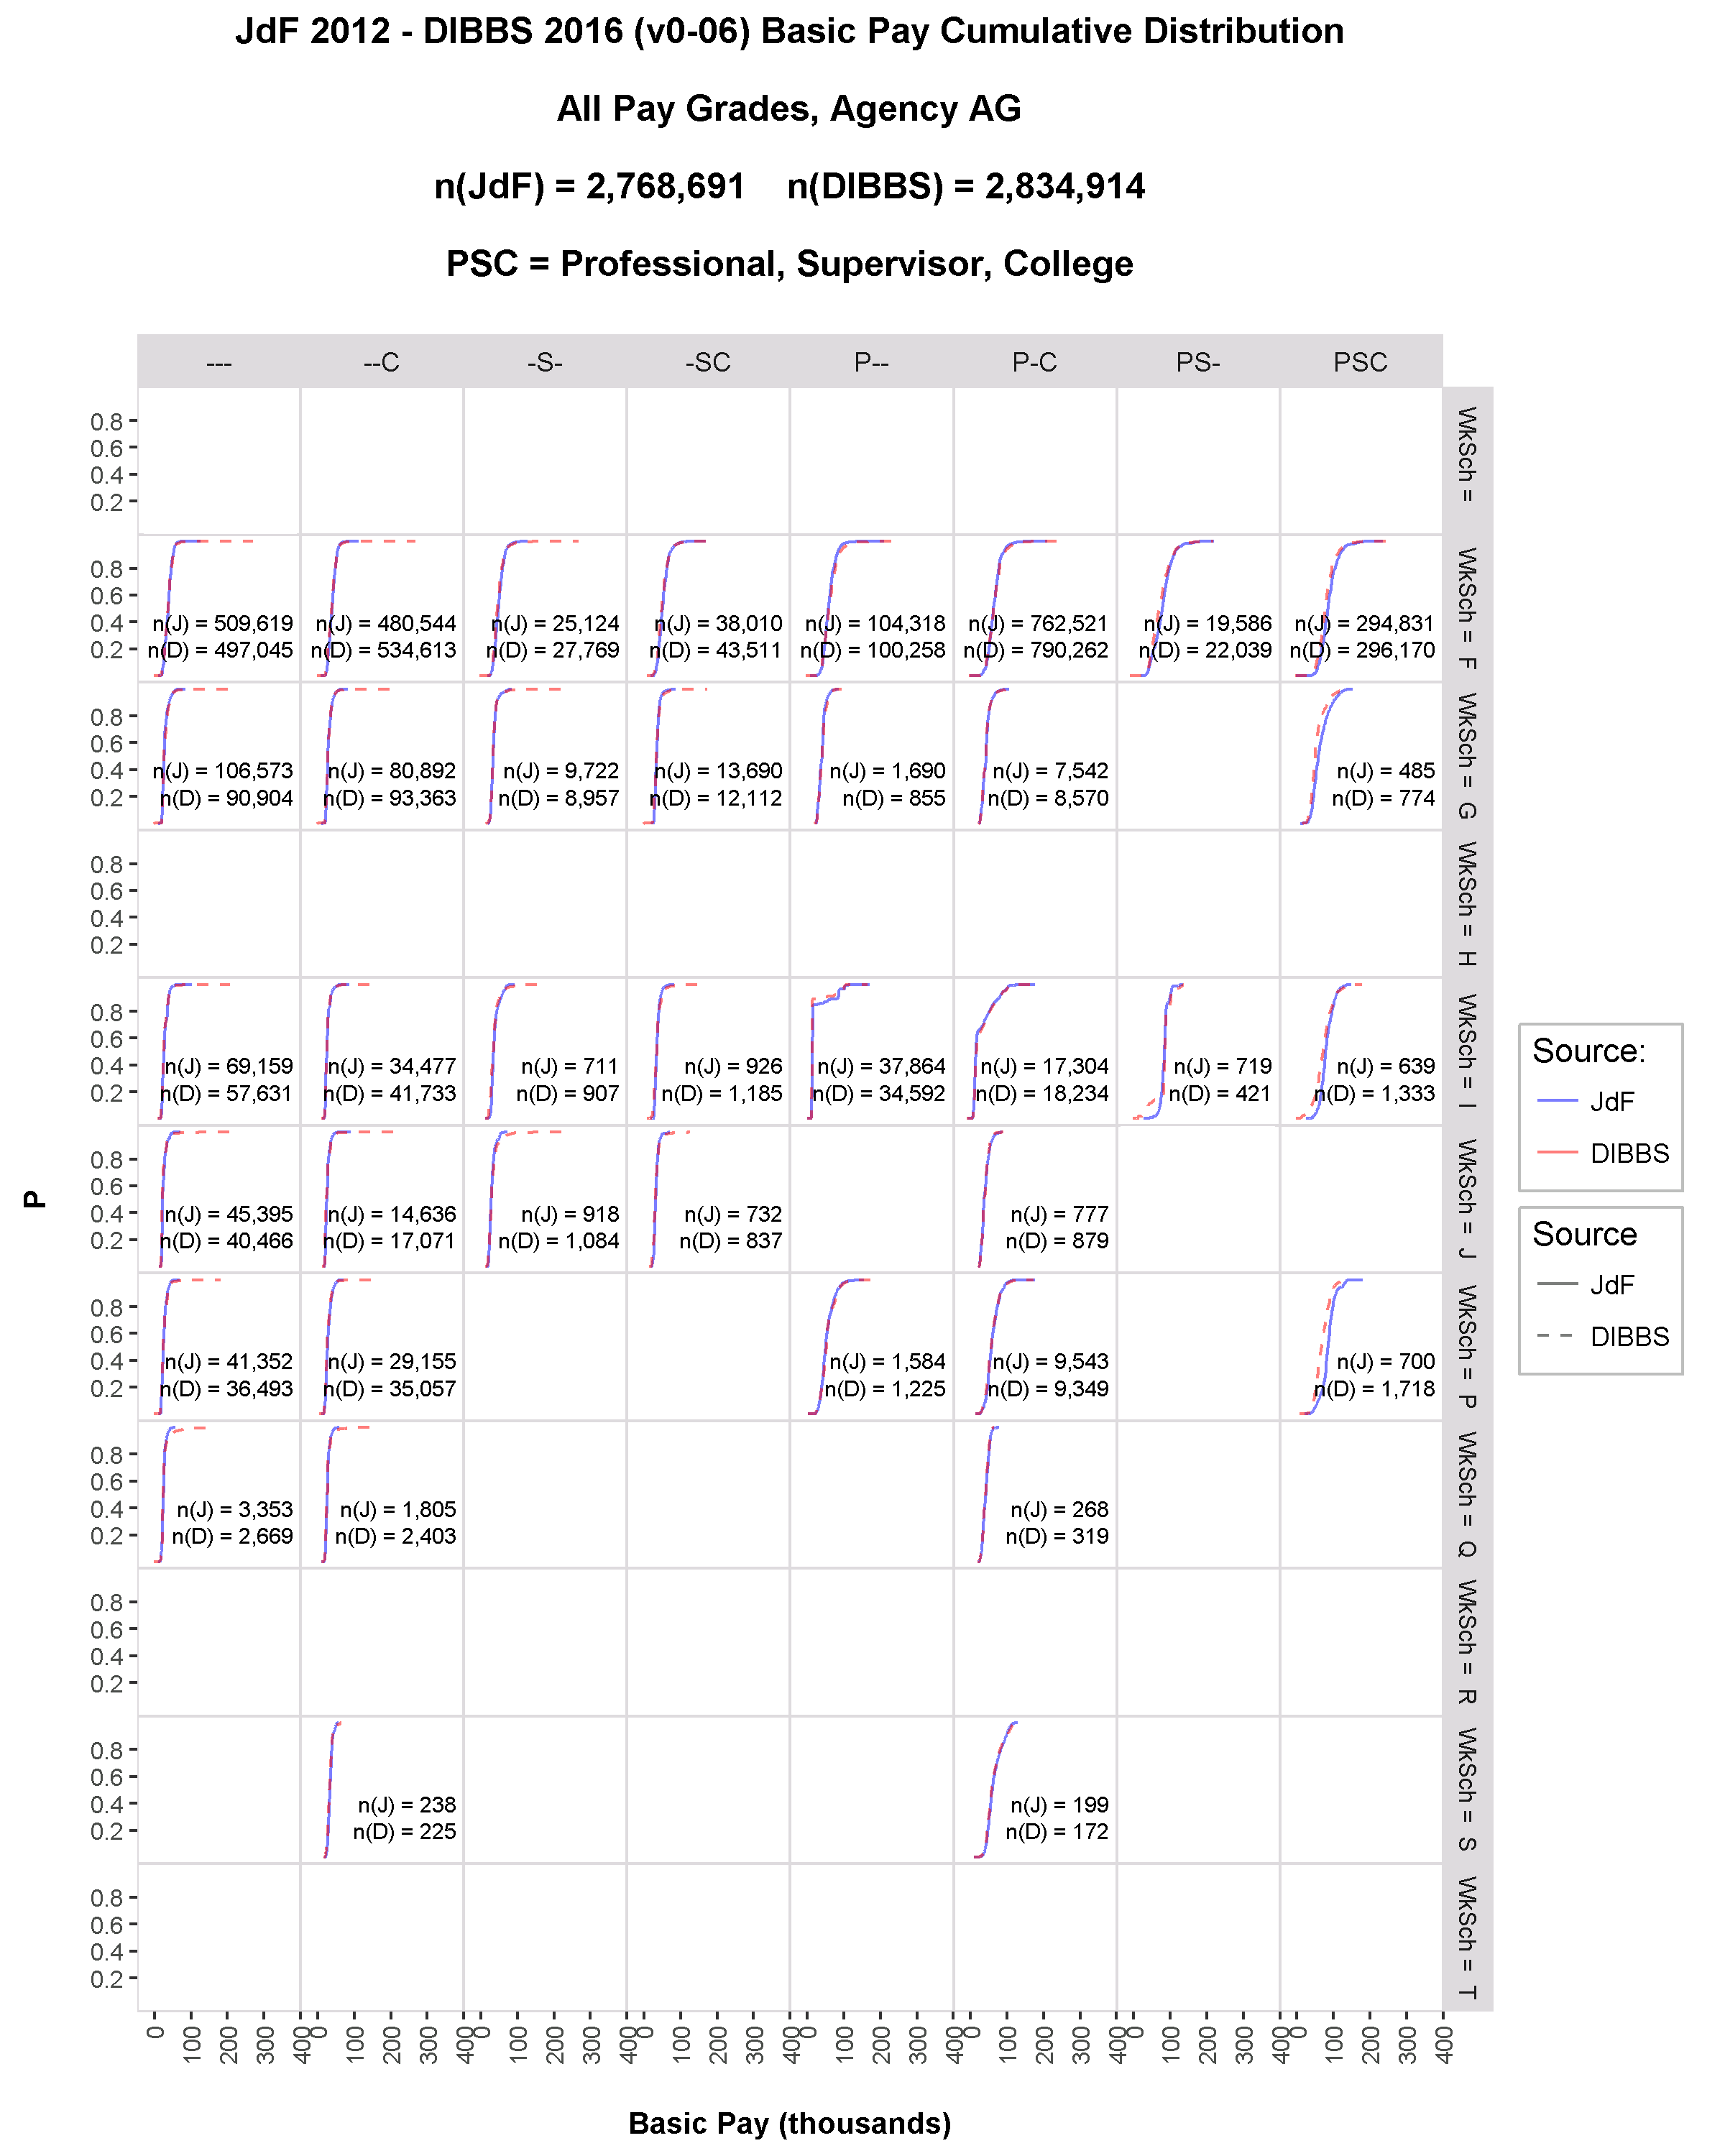
\includegraphics[width=6.5in, trim={0 0 1in 1.5in}, clip]{JdFDIBBSBasicPayCDFAG.png}
    \caption{Basic pay distribution by joint professional, supervisory status, college education, and work schedule  categories.  Department of Agriculture (AG).  Dashed line for synthetic data, solid line for authentic.}
    \label{figure:JdFDIBBSBasicPayCDFAG}
\end{figure}

\clearpage

\begin{figure}[h]
    \centering
    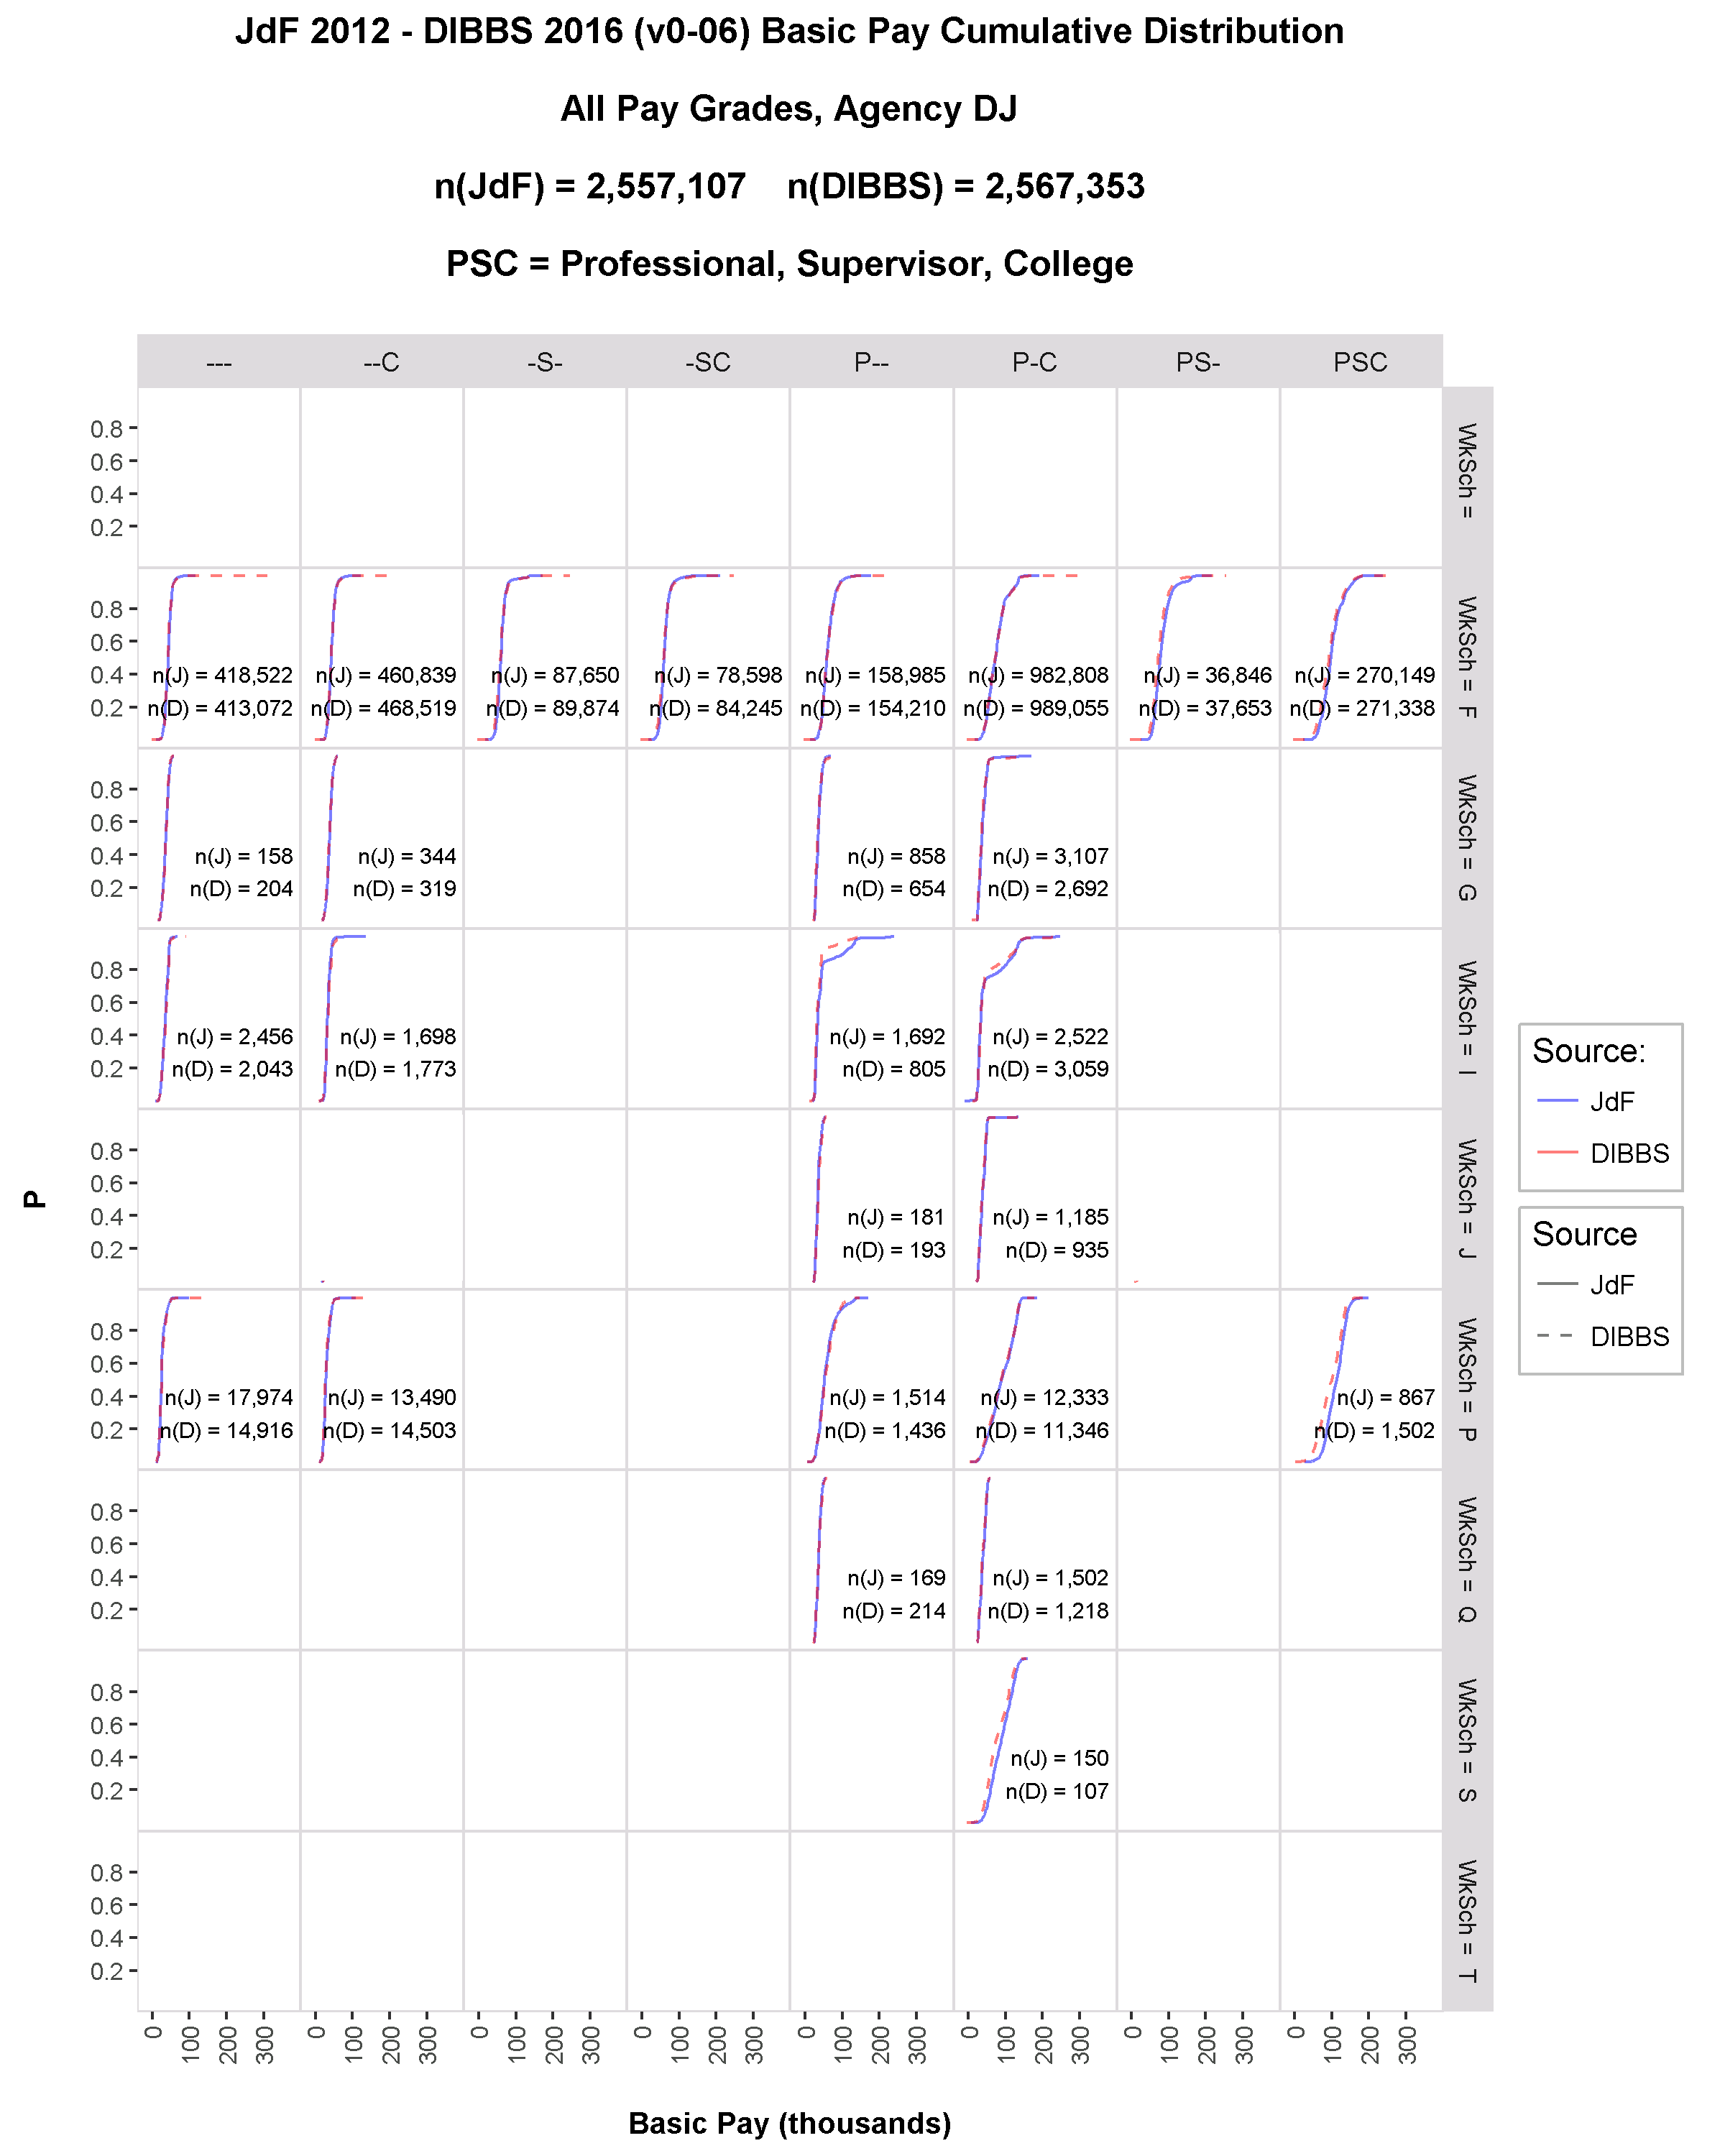
\includegraphics[width=6.5in, trim={0 0 1in 1.5in}, clip]{JdFDIBBSBasicPayCDFDJ.png}
    \caption{Basic pay distribution by joint professional, supervisory status, college education, and work schedule  categories.  Department of Justice (DJ).  Dashed line for synthetic data, solid line for authentic.}
    \label{figure:JdFDIBBSBasicPayCDFDJ}
\end{figure}

\clearpage

\begin{figure}[h]
    \centering
    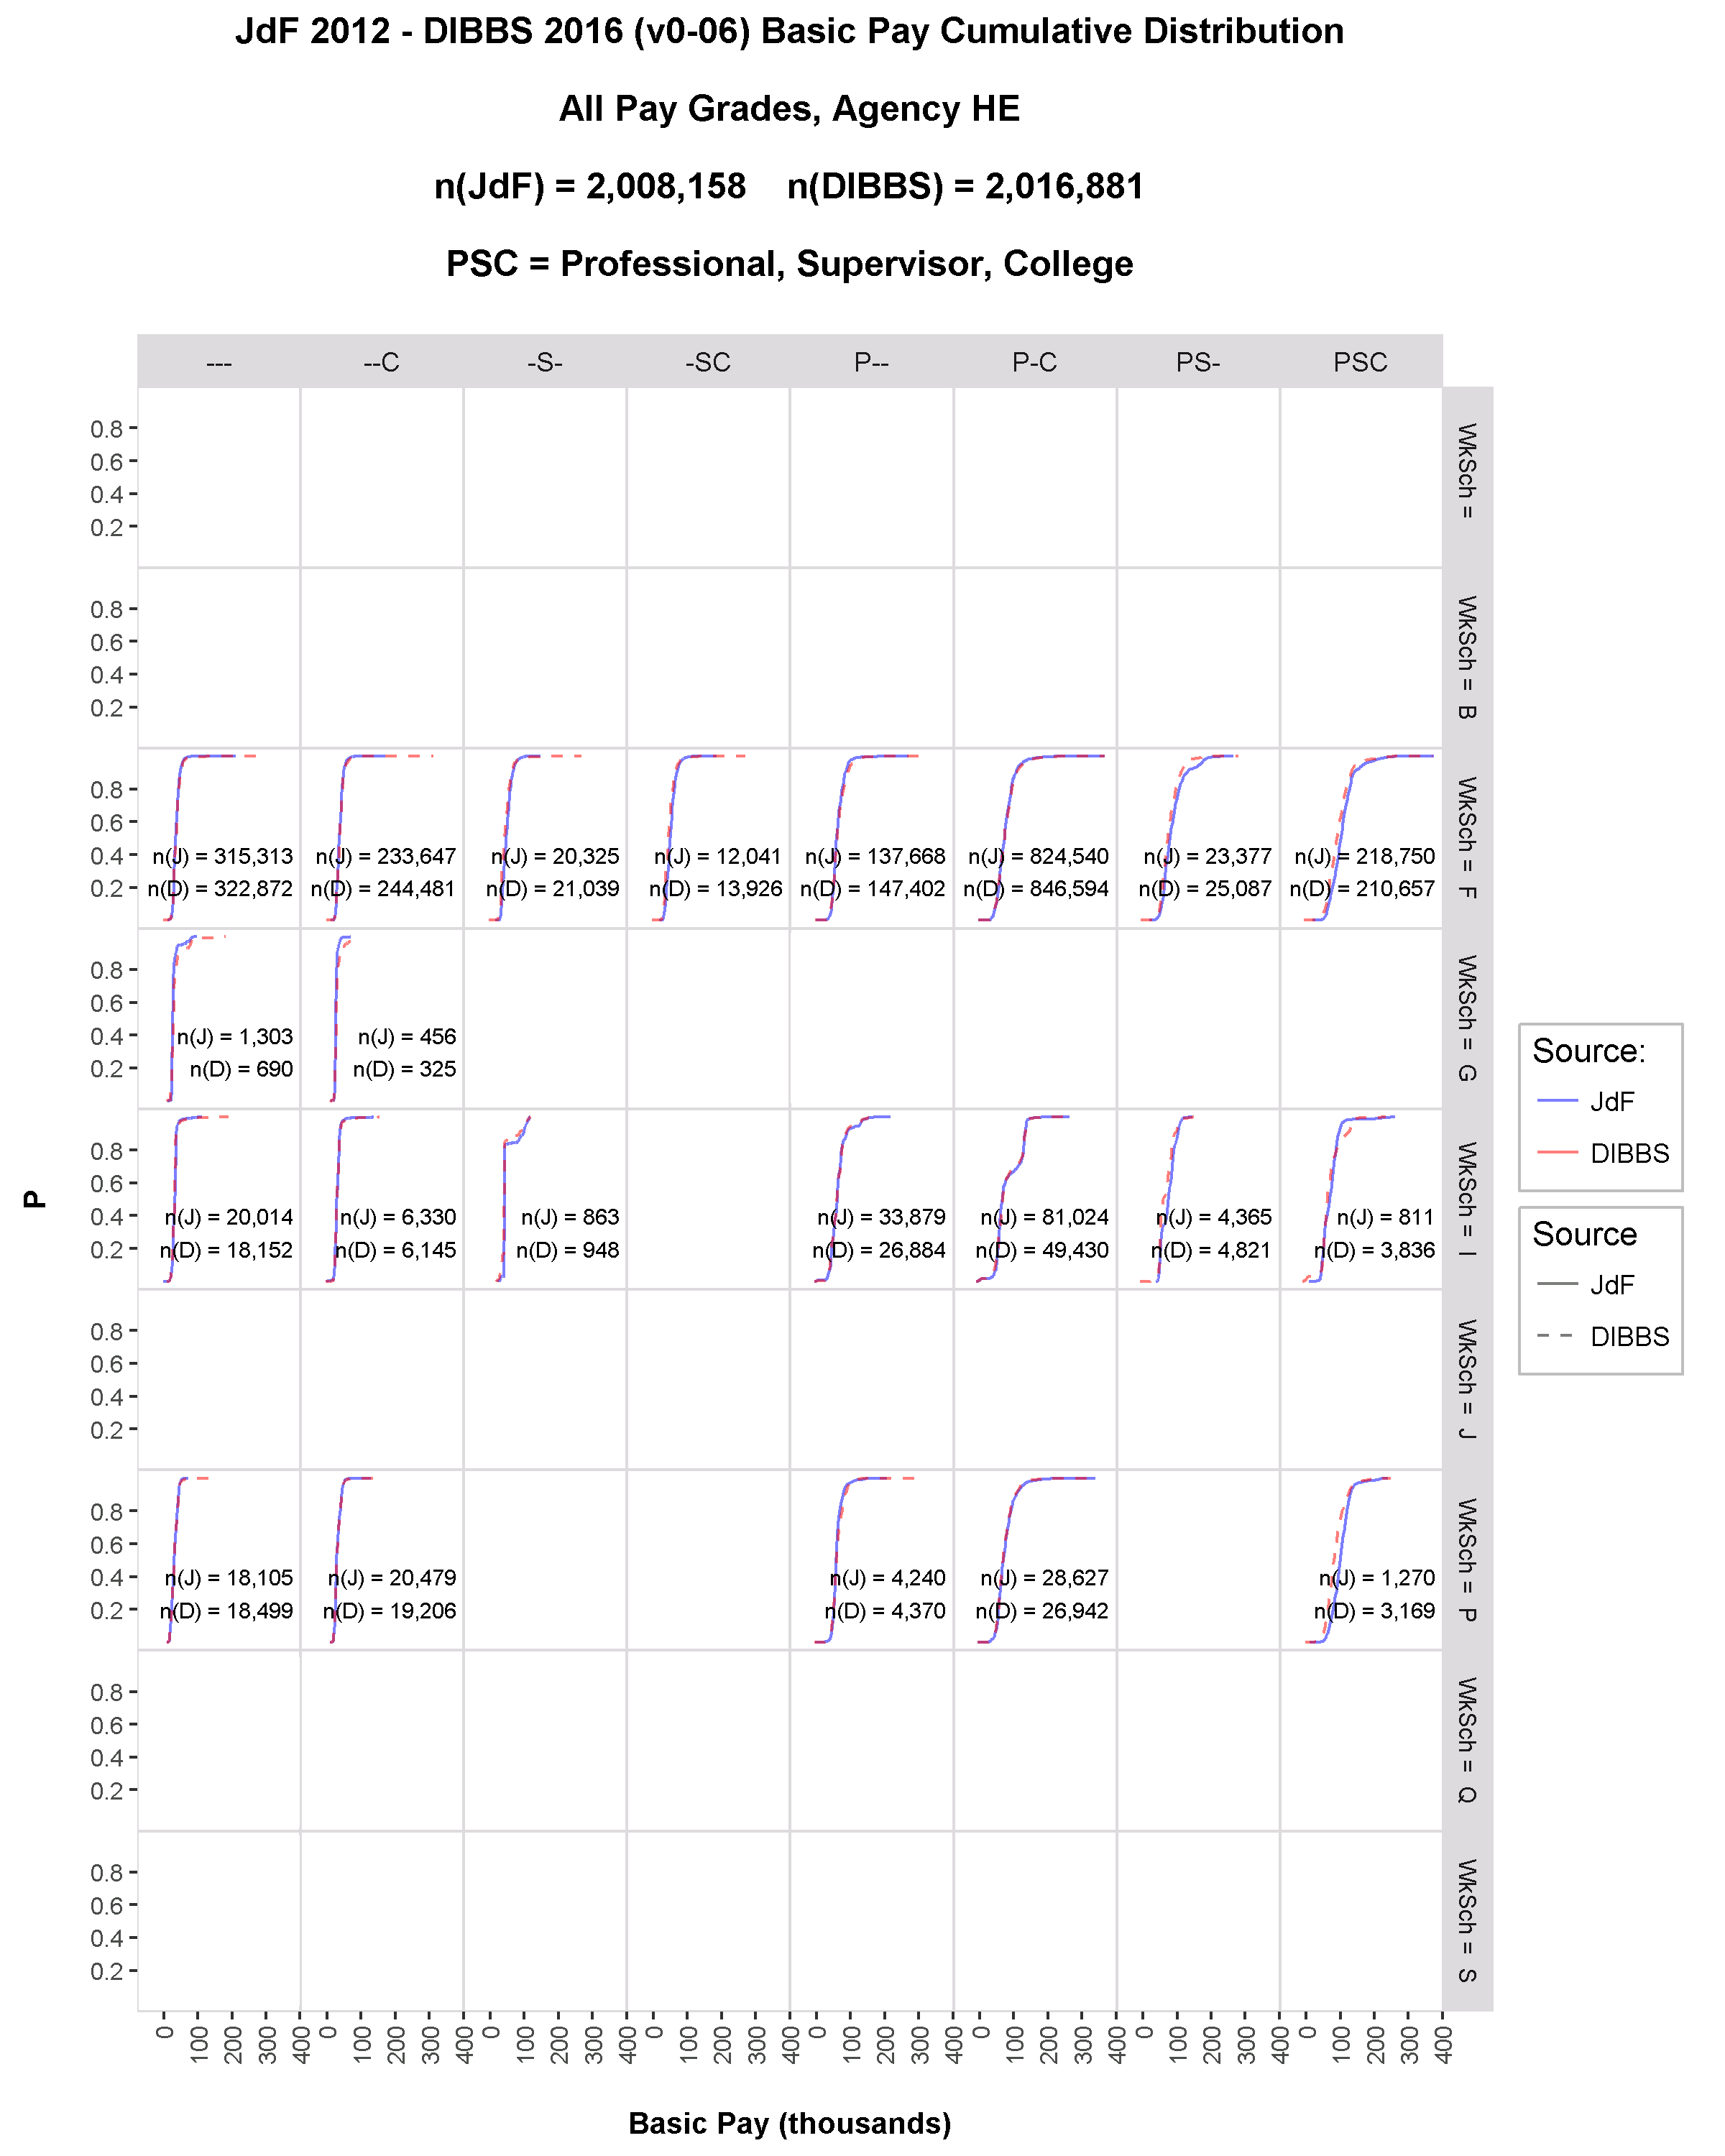
\includegraphics[width=6.5in, trim={0 0 1in 1.5in}, clip]{JdFDIBBSBasicPayCDFHE.png}
    \caption{Basic pay distribution by joint professional, supervisory status, college education, and work schedule  categories.  Department of Health and Human Services (HE).  Dashed line for synthetic data, solid line for authentic.}
    \label{figure:JdFDIBBSBasicPayCDFHE}
\end{figure}

\clearpage

\begin{figure}[h]
    \centering
    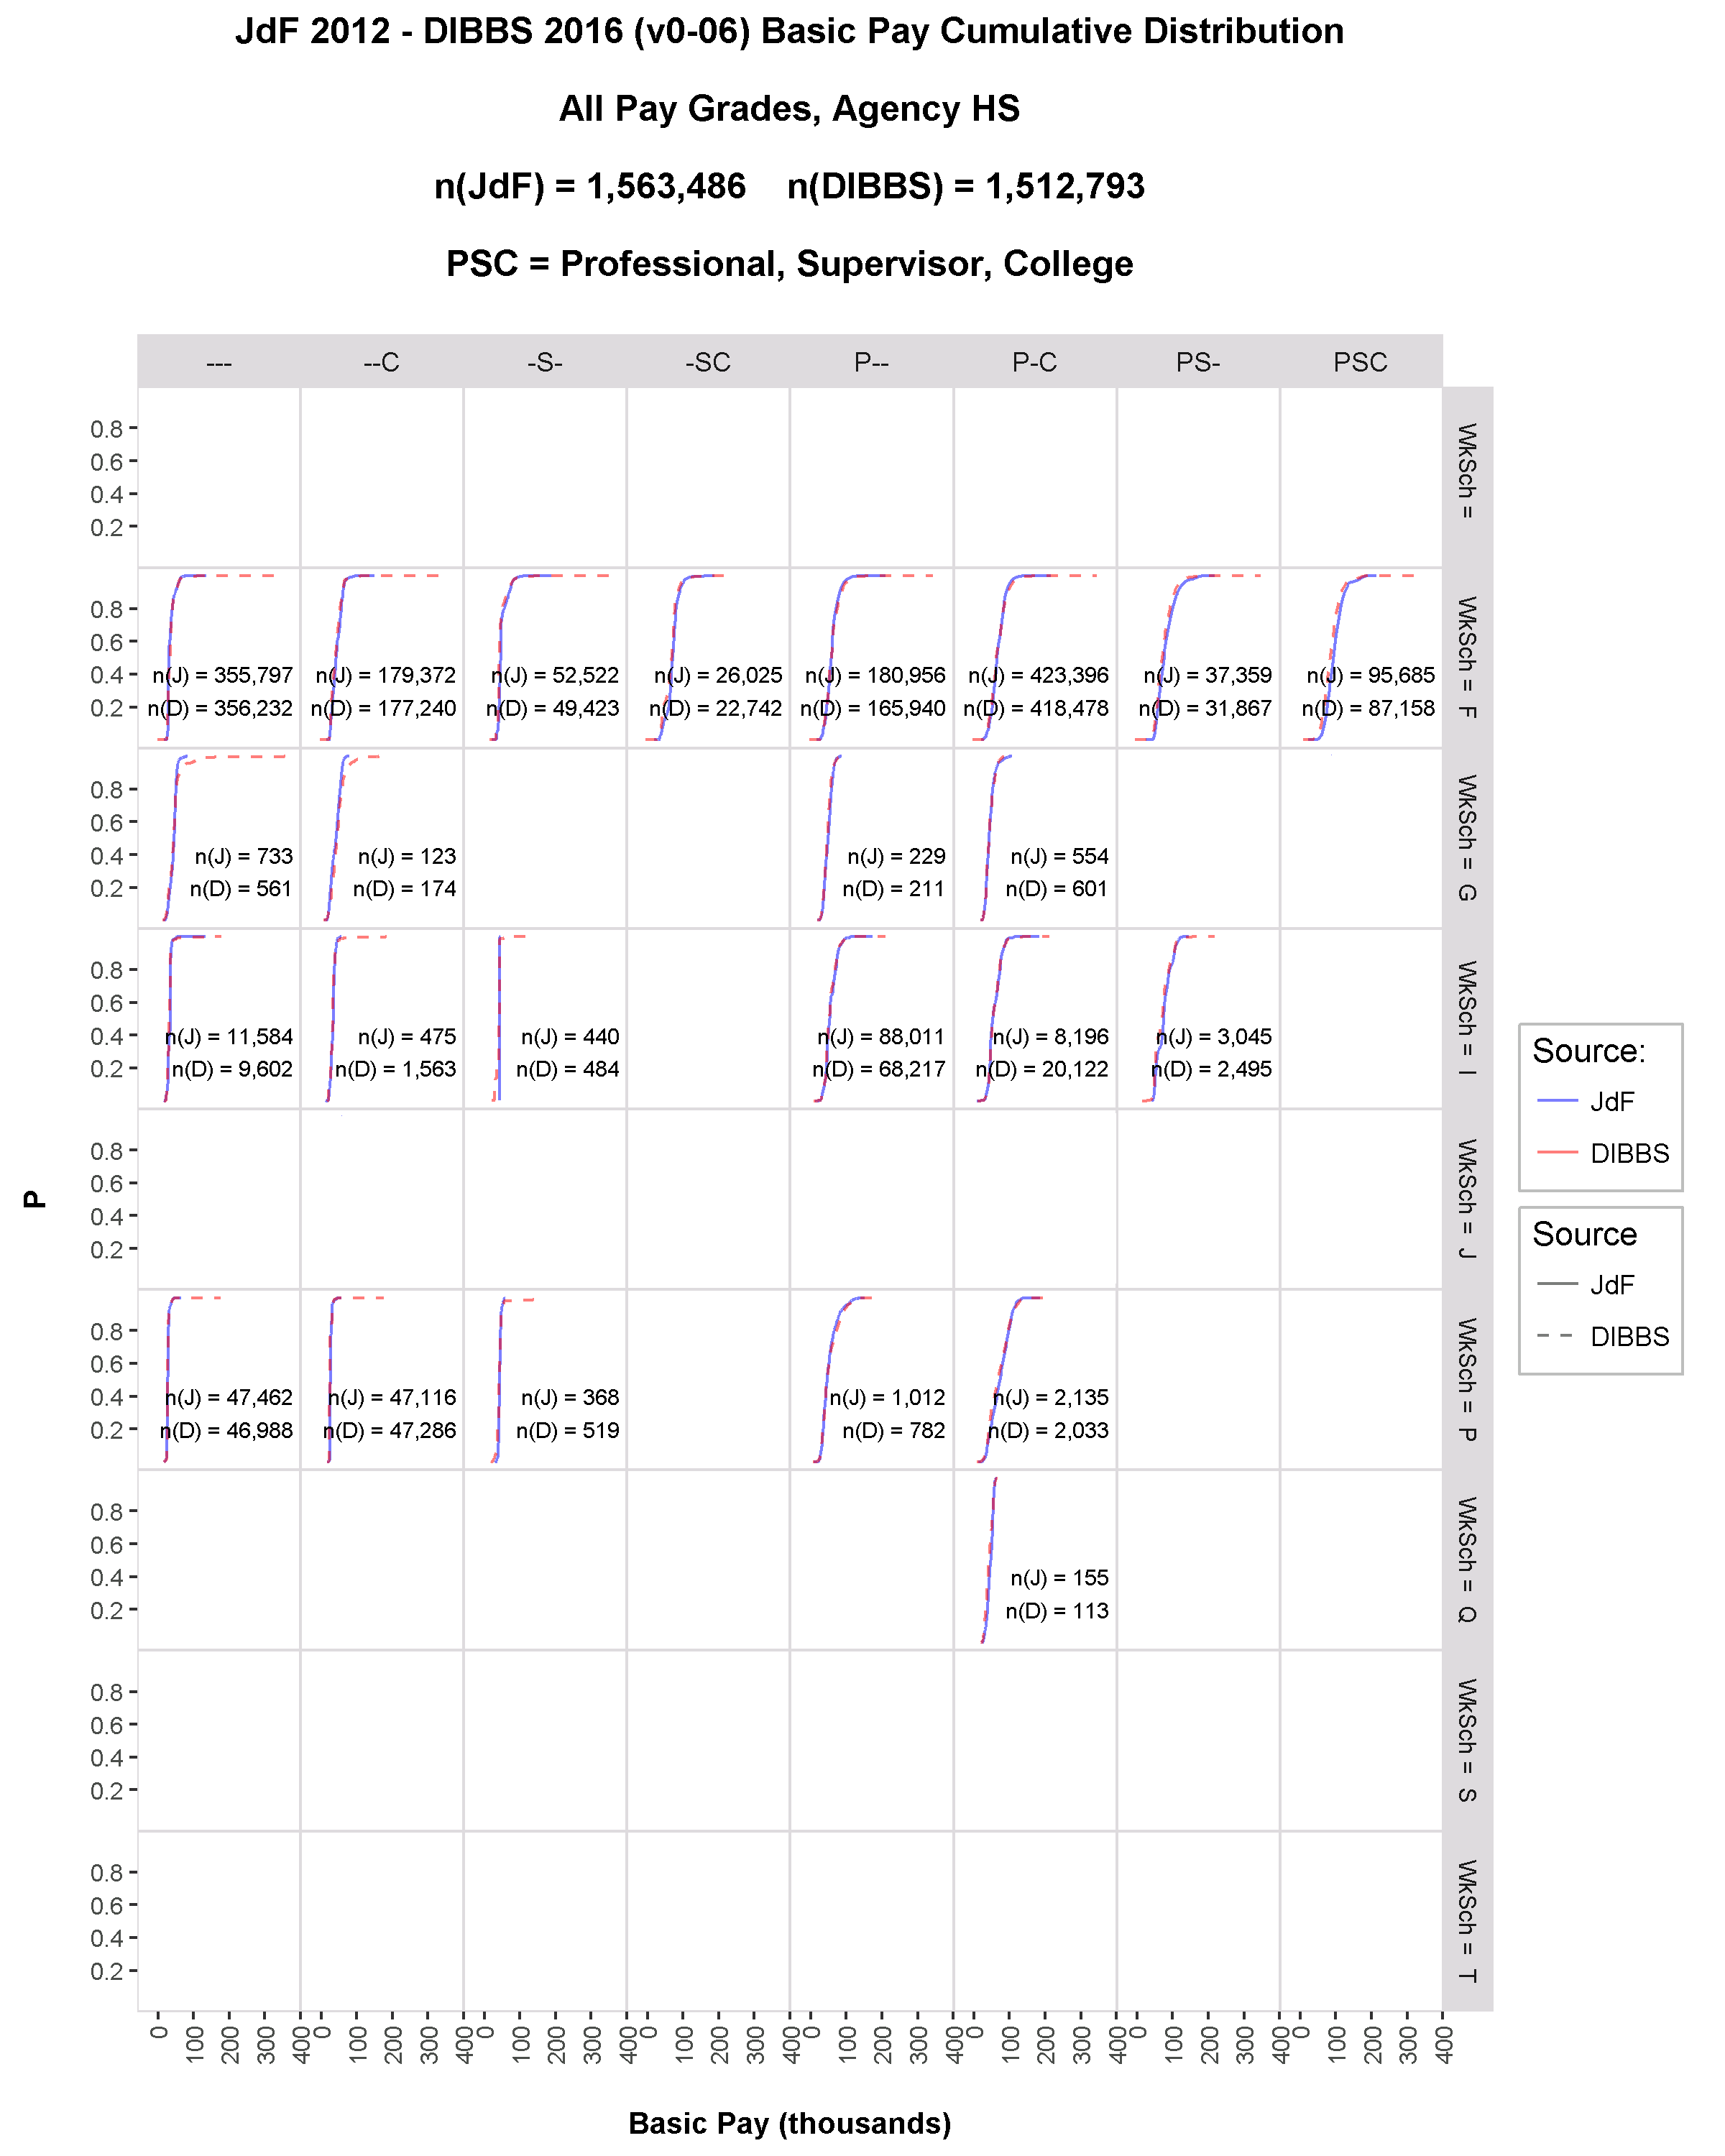
\includegraphics[width=6.5in, trim={0 0 1in 1.5in}, clip]{JdFDIBBSBasicPayCDFHS.png}
    \caption{Basic pay distribution by joint professional, supervisory status, college education, and work schedule  categories.  Department of Homeland Security (HS).  Dashed line for synthetic data, solid line for authentic.}
    \label{figure:JdFDIBBSBasicPayCDFHS}
\end{figure}

\clearpage

\begin{figure}[h]
    \centering
    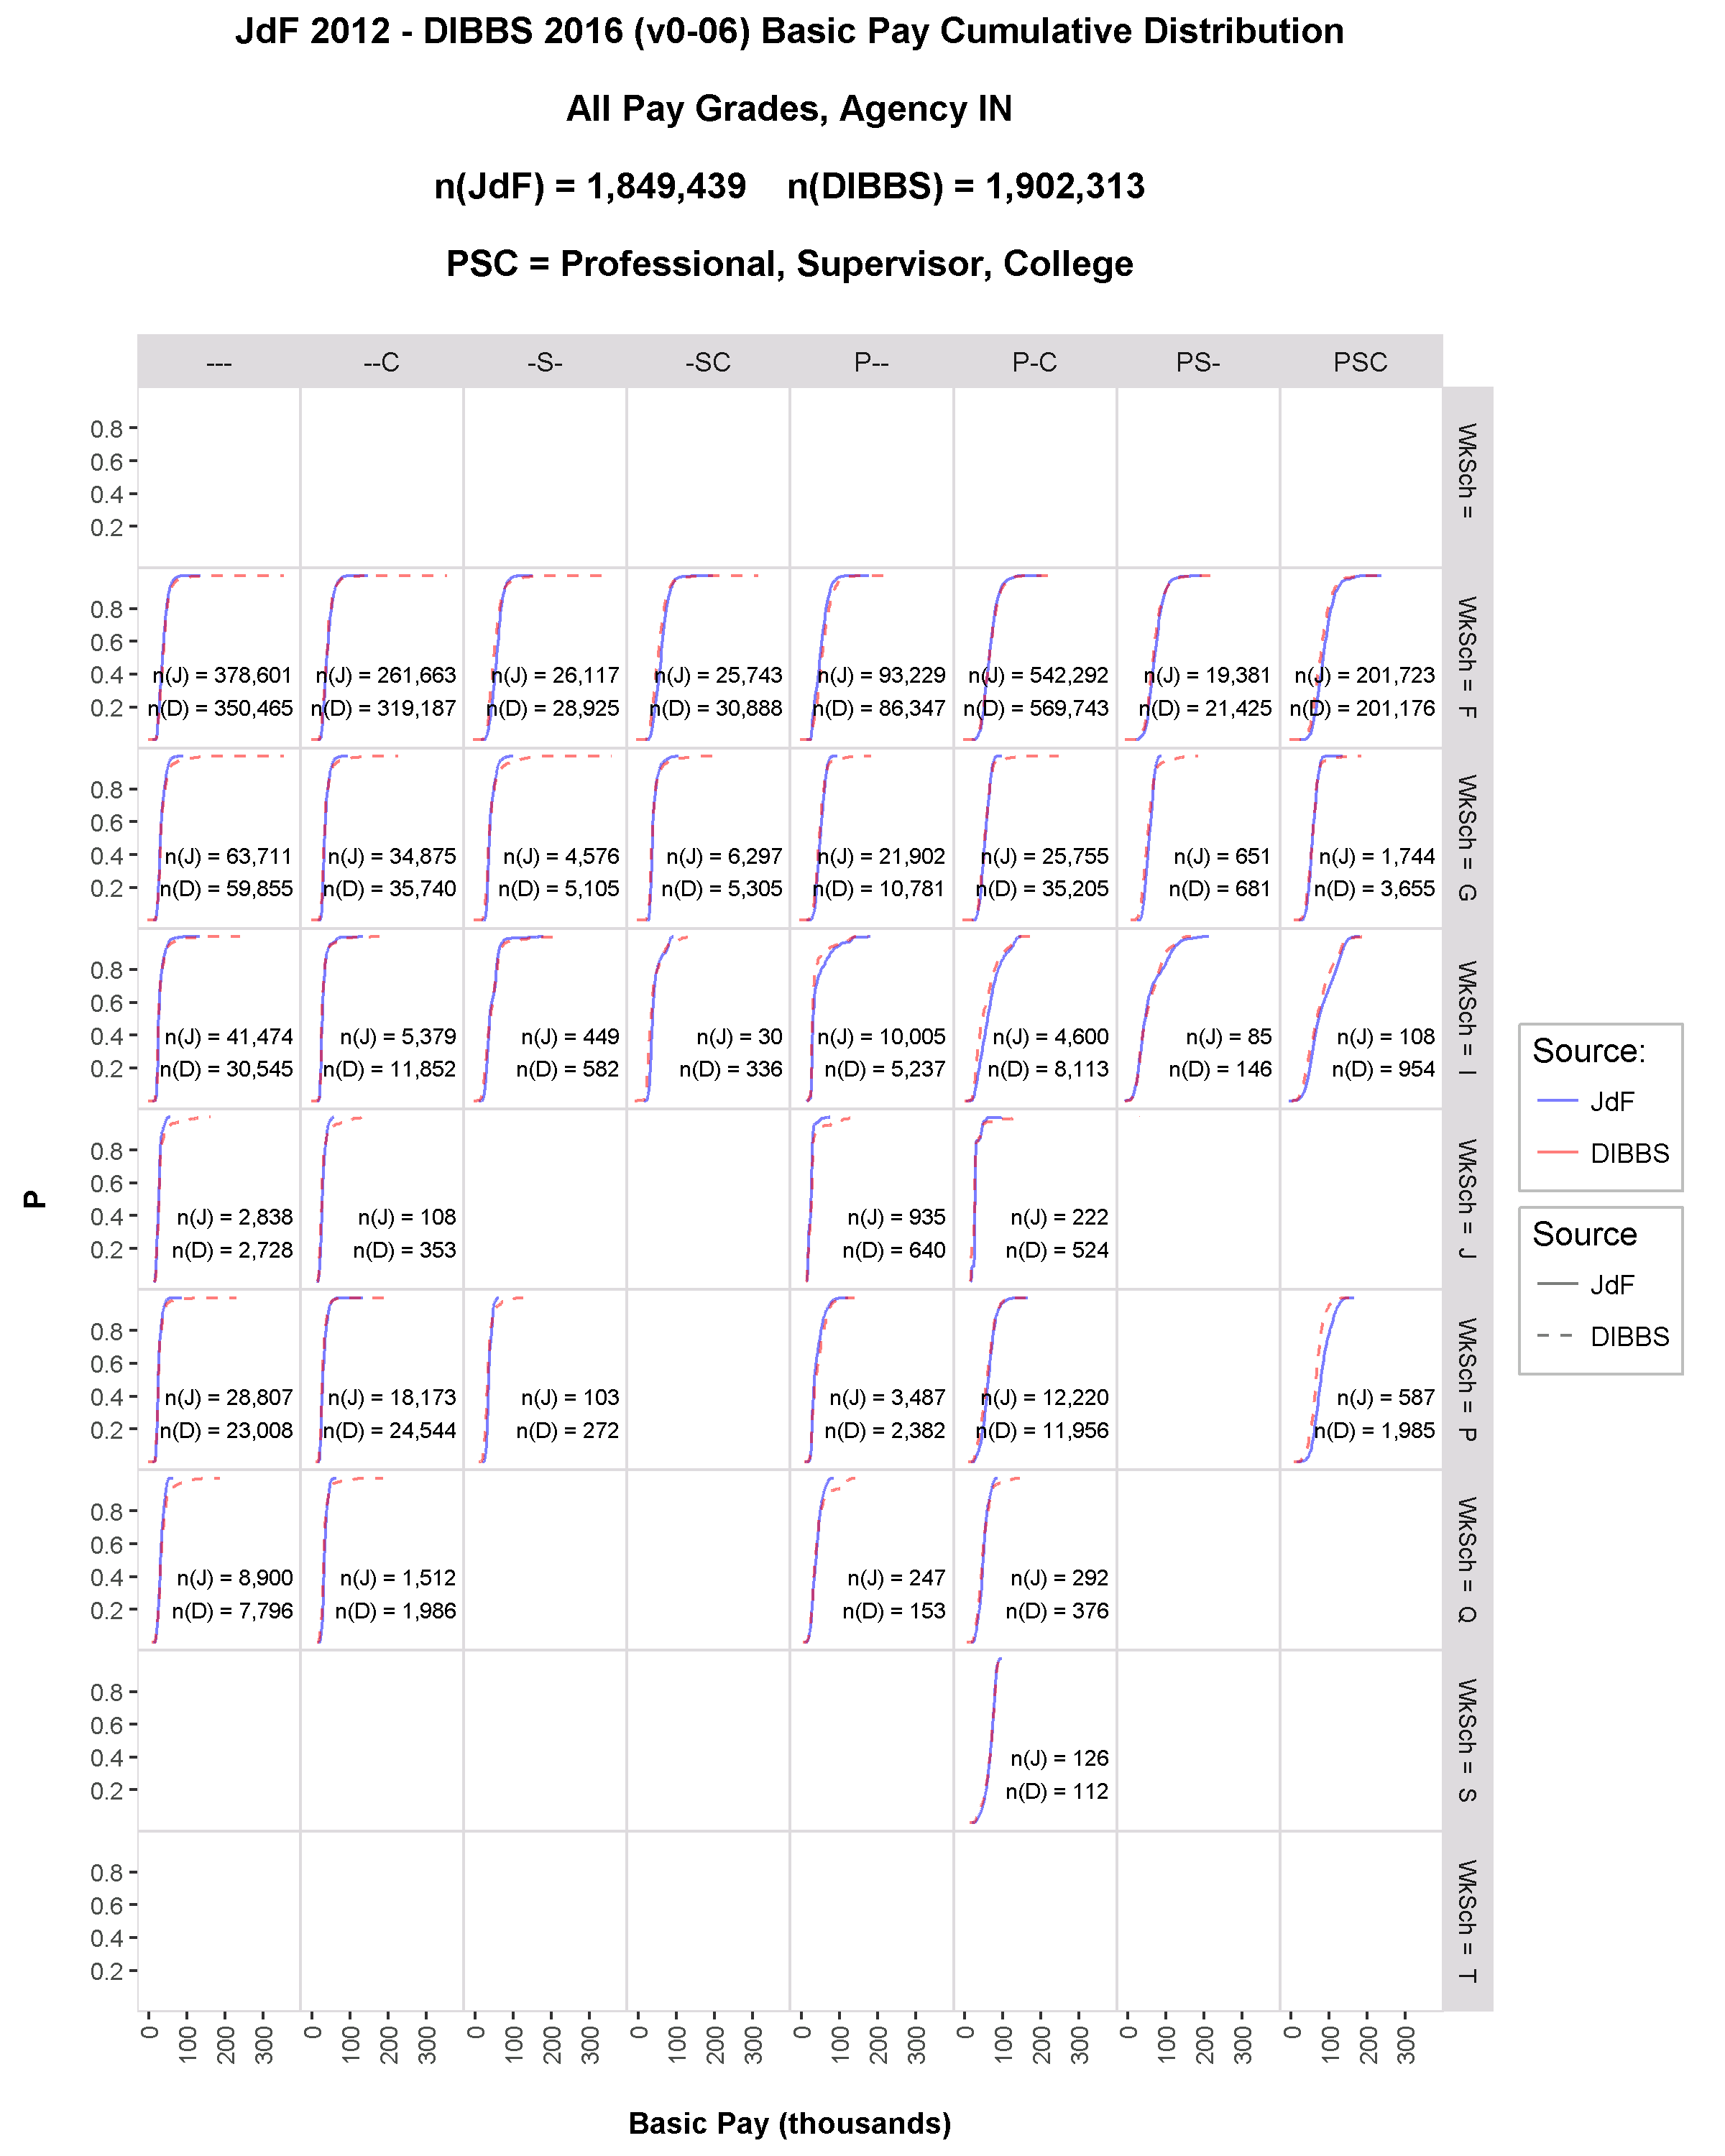
\includegraphics[width=6.5in, trim={0 0 1in 1.5in}, clip]{JdFDIBBSBasicPayCDFIN.png}
    \caption{Basic pay distribution by joint professional, supervisory status, college education, and work schedule  categories.  Department of Interior (IN).  Dashed line for synthetic data, solid line for authentic.}
    \label{figure:JdFDIBBSBasicPayCDFIN}
\end{figure}

\clearpage

\begin{figure}[h]
    \centering
    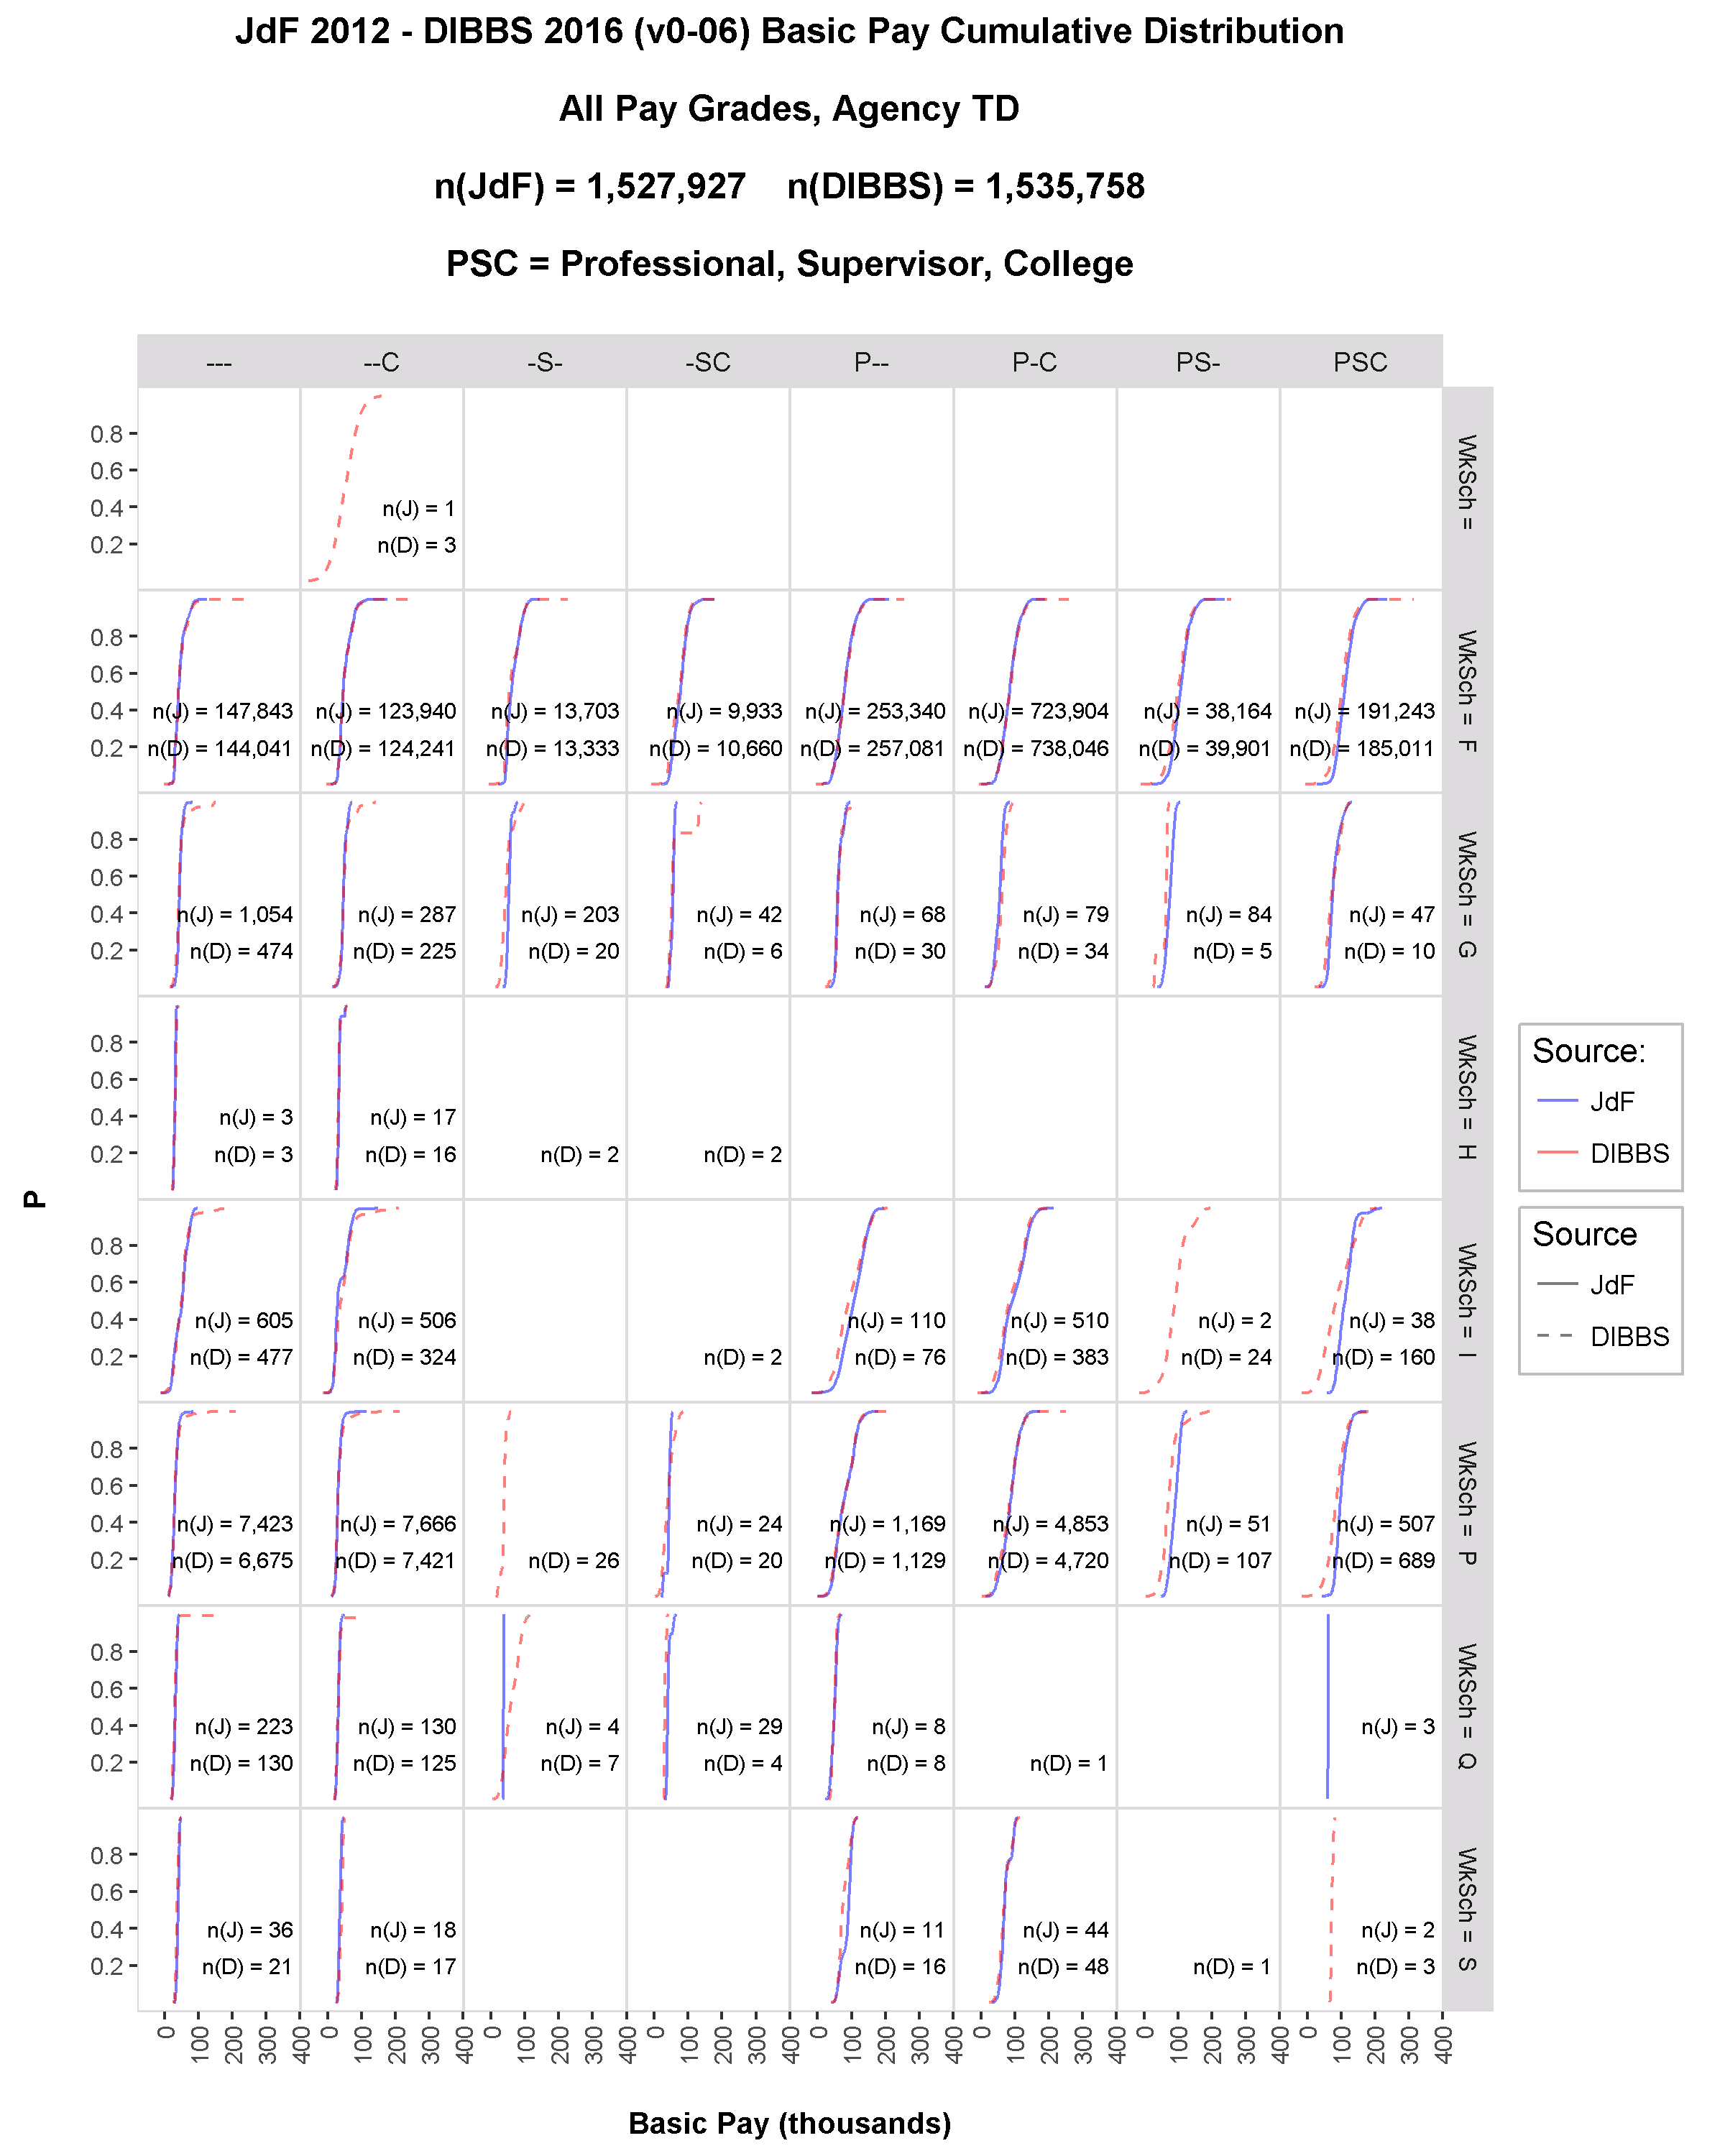
\includegraphics[width=6.5in, trim={0 0 1in 1.5in}, clip]{JdFDIBBSBasicPayCDFTD.png}
    \caption{Basic pay distribution by joint professional, supervisory status, college education, and work schedule  categories.  Department of Transportation (TD).  Dashed line for synthetic data, solid line for authentic.}
    \label{figure:JdFDIBBSBasicPayCDFTD}
\end{figure}

\clearpage

\begin{figure}[h]
    \centering
    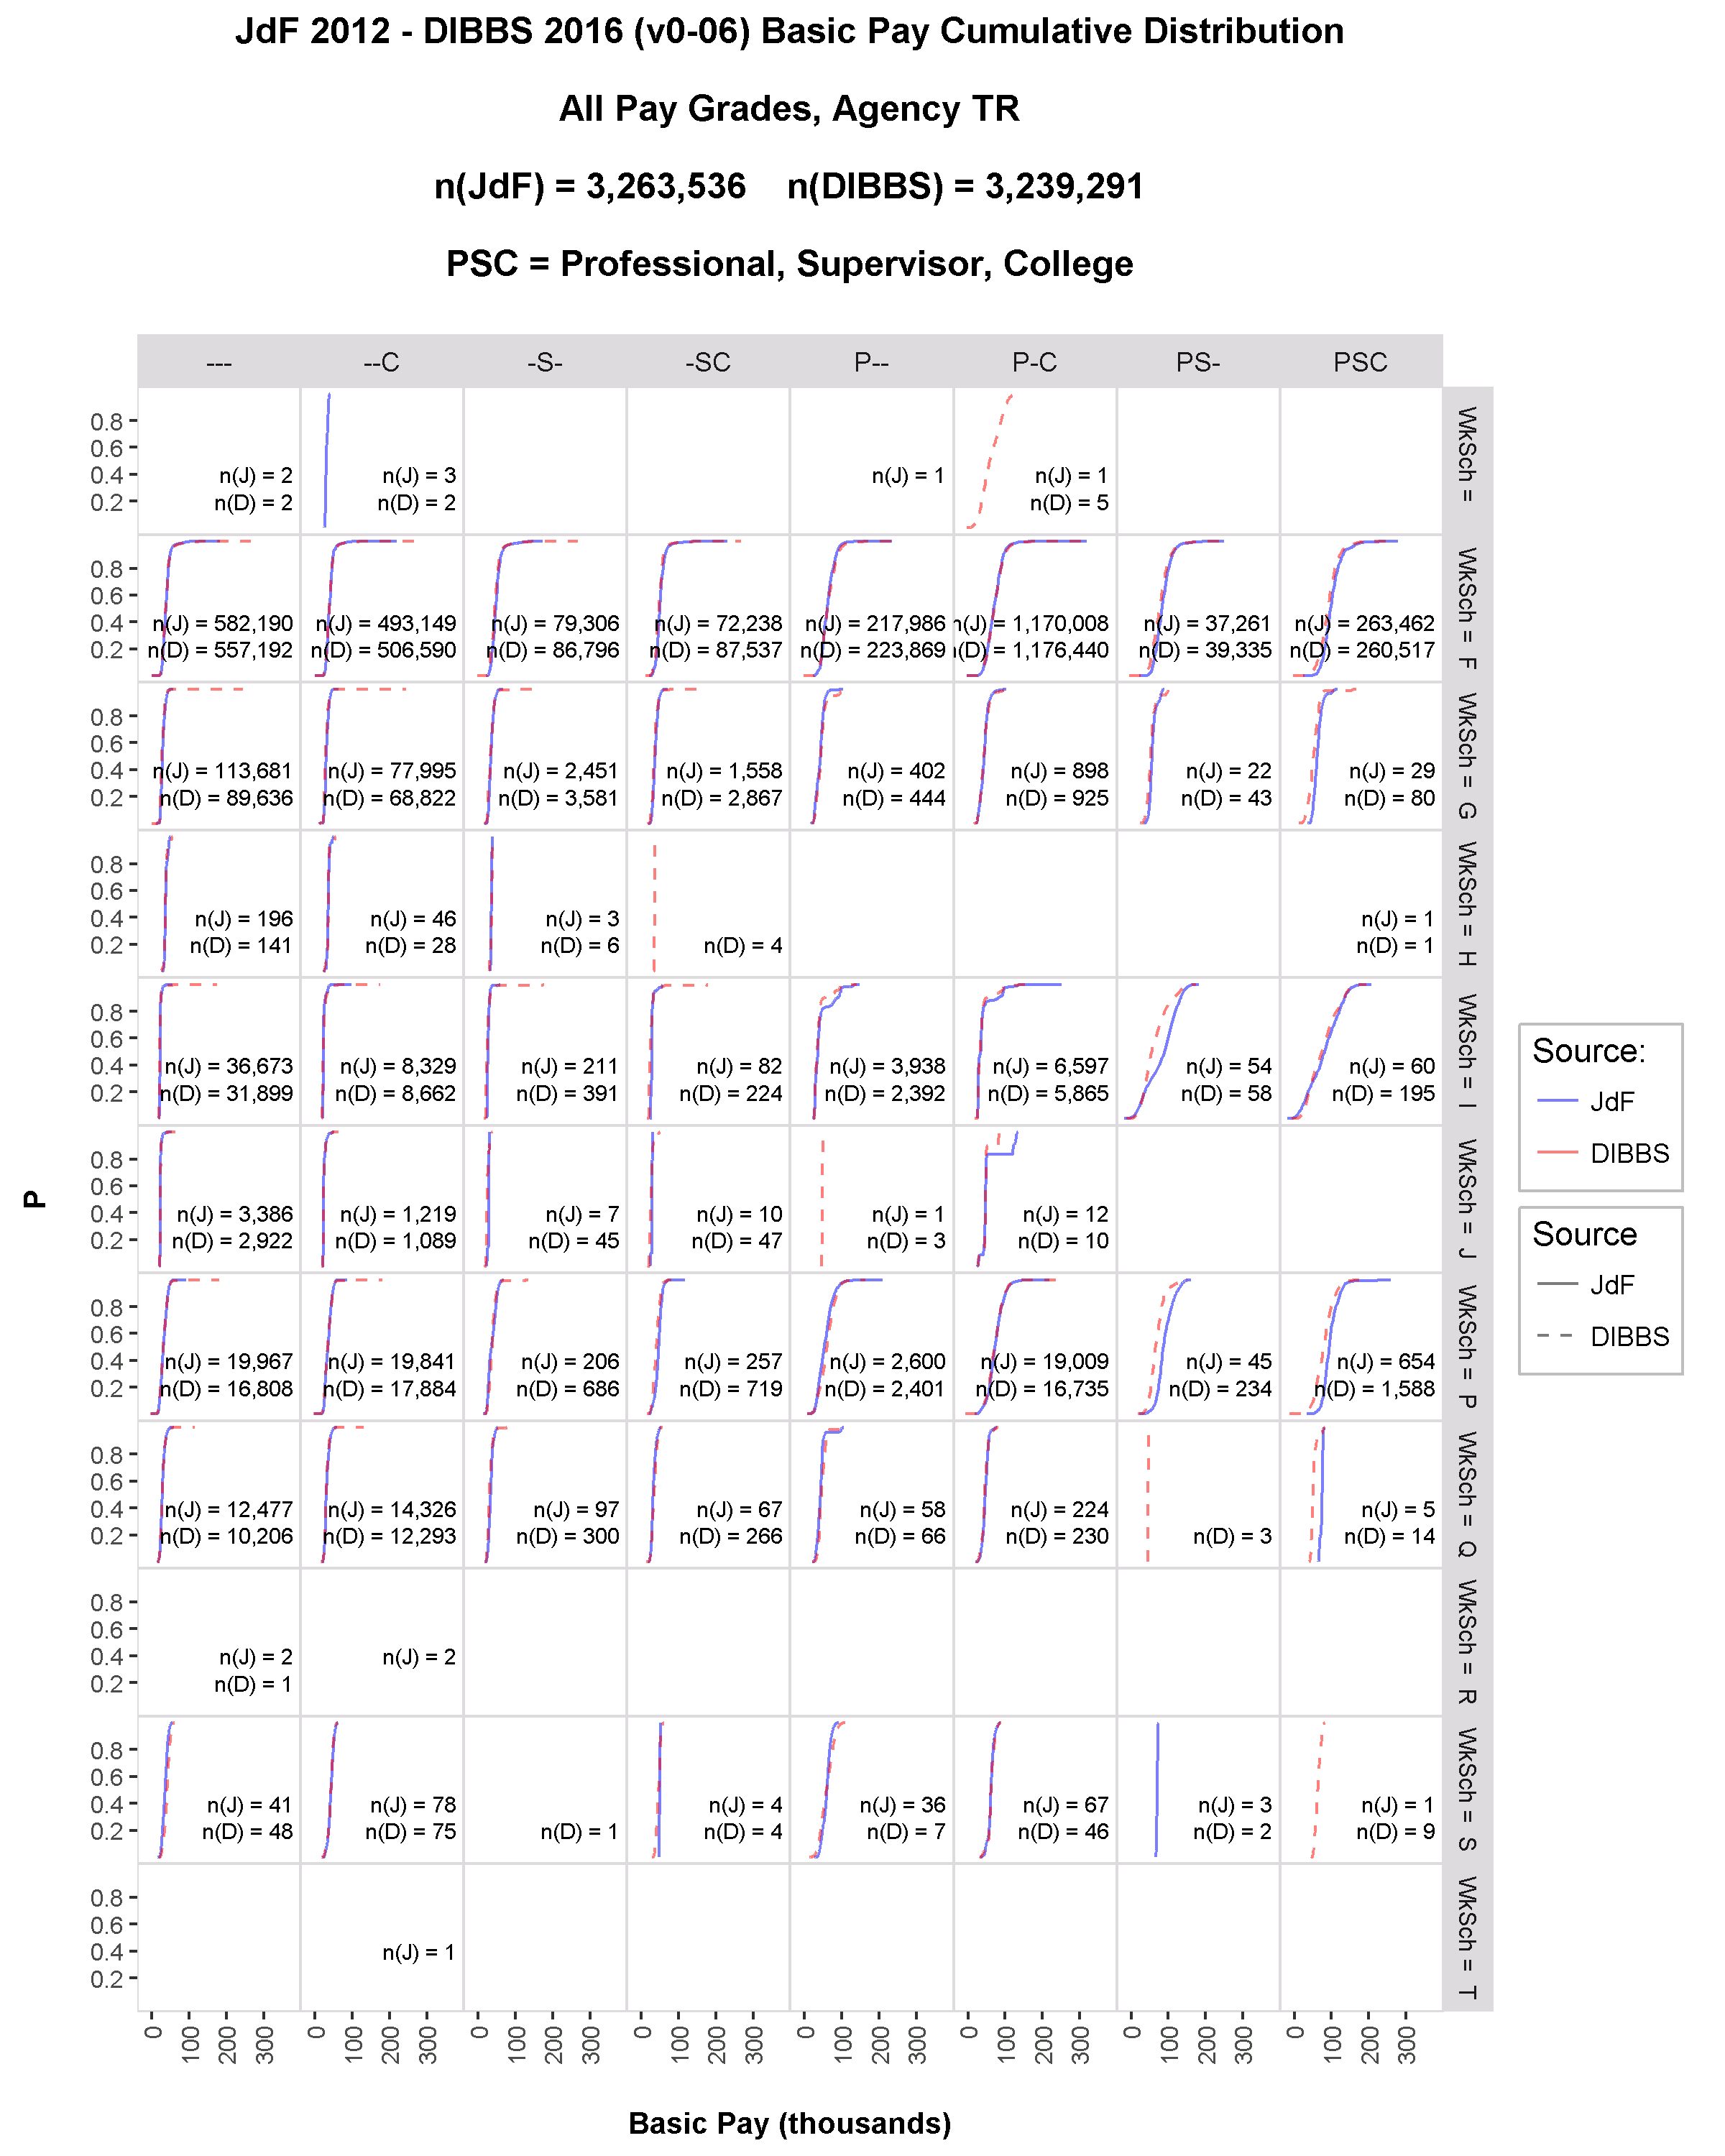
\includegraphics[width=6.5in, trim={0 0 1in 1.5in}, clip]{JdFDIBBSBasicPayCDFTR.png}
    \caption{Basic pay distribution by joint professional, supervisory status, college education, and work schedule  categories.  Department of Treasury (TR).  Dashed line for synthetic data, solid line for authentic.}
    \label{figure:JdFDIBBSBasicPayCDFTR}
\end{figure}

\clearpage

\begin{figure}[h]
    \centering
    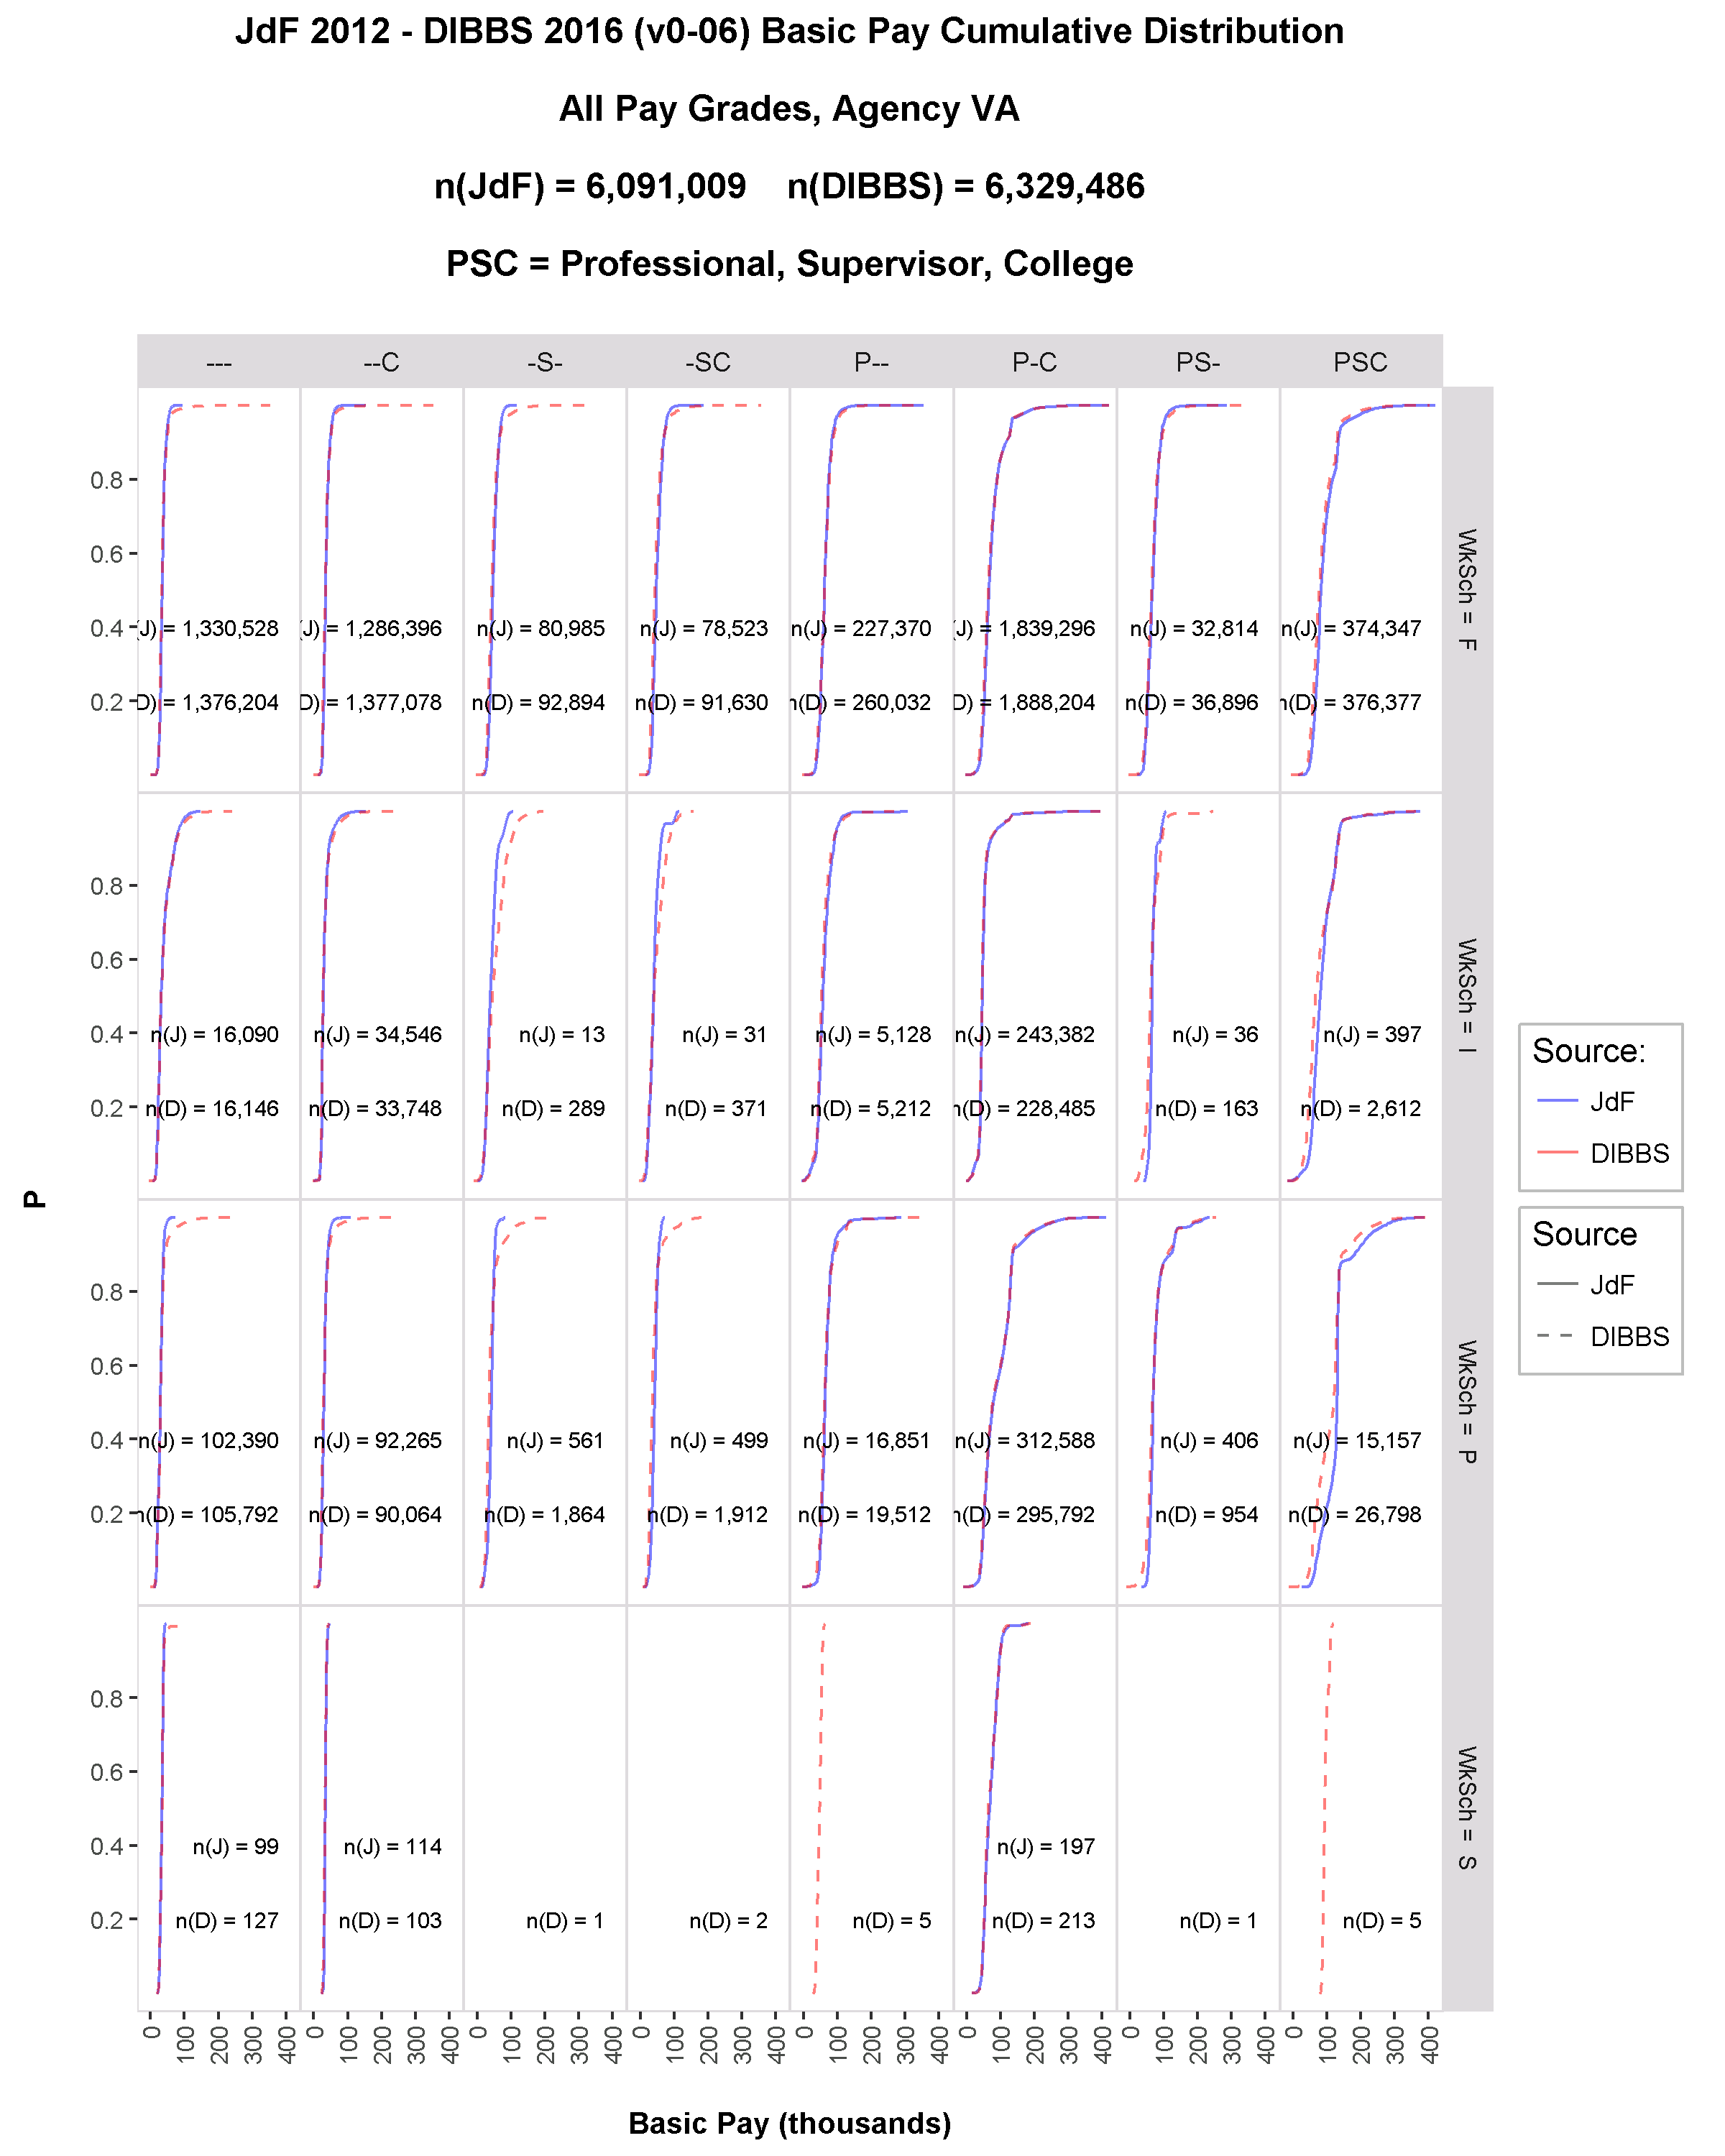
\includegraphics[width=6.5in, trim={0 0 1in 1.5in}, clip]{JdFDIBBSBasicPayCDFVA.png}
    \caption{Basic pay distribution by joint professional, supervisory status, college education, and work schedule  categories.  Department of Veterans Affairs (VA).  Dashed line for synthetic data, solid line for authentic.}
    \label{figure:JdFDIBBSBasicPayCDFVA}
\end{figure}

\clearpage

\subsection{Distribution of Basic Pay by Occupation and Supervisory Status}

803 distinct occupations are represented in the data supplied by OPM.  To verify distribution of basic pay by occupation and supervisory status in the synthetic data, box plots consisting of a pair of authentic/synthetic distributions for each occupation were constructed.  Figures \ref{figure:JdFDIBBSBasicPaySupervisoryStatusOccupation1} through \ref{figure:JdFDIBBSBasicPaySupervisoryStatusOccupation3} show box plots for the first 120 occupations in order of occupation code.  Trade, or blue collar, occupations begin at code 2500.  Figures \ref{figure:JdFDIBBSBasicPaySupervisoryStatusOccupation4} and \ref{figure:JdFDIBBSBasicPaySupervisoryStatusOccupation5} show the distributions of the first 80 of these occupations.  Remaining occupations exhibit patterns similar to those presented.\\

Observations:  Median pay and inter-quartile ranges appear consistent between data sets.  Upper tails of distributions of in the synthetic data generally appear greater than corresponding authentic distributions, particulary for trade occupations.  Note that, of the 318 trade occupations represented in the authentic data, 190 have proportion female observations less than 0.05.  Given disparity in federal employee pay by gender \citep{BoltondeFigGenderPayGap2017} and a requirement, for protection of privacy, of a degree of modification of gender and occupation in synthetic observations, some difference in pay extremes may be expected.\\

\begin{figure}[h]
    \centering
    \begin{subfigure}{1\textwidth}
        \centering
        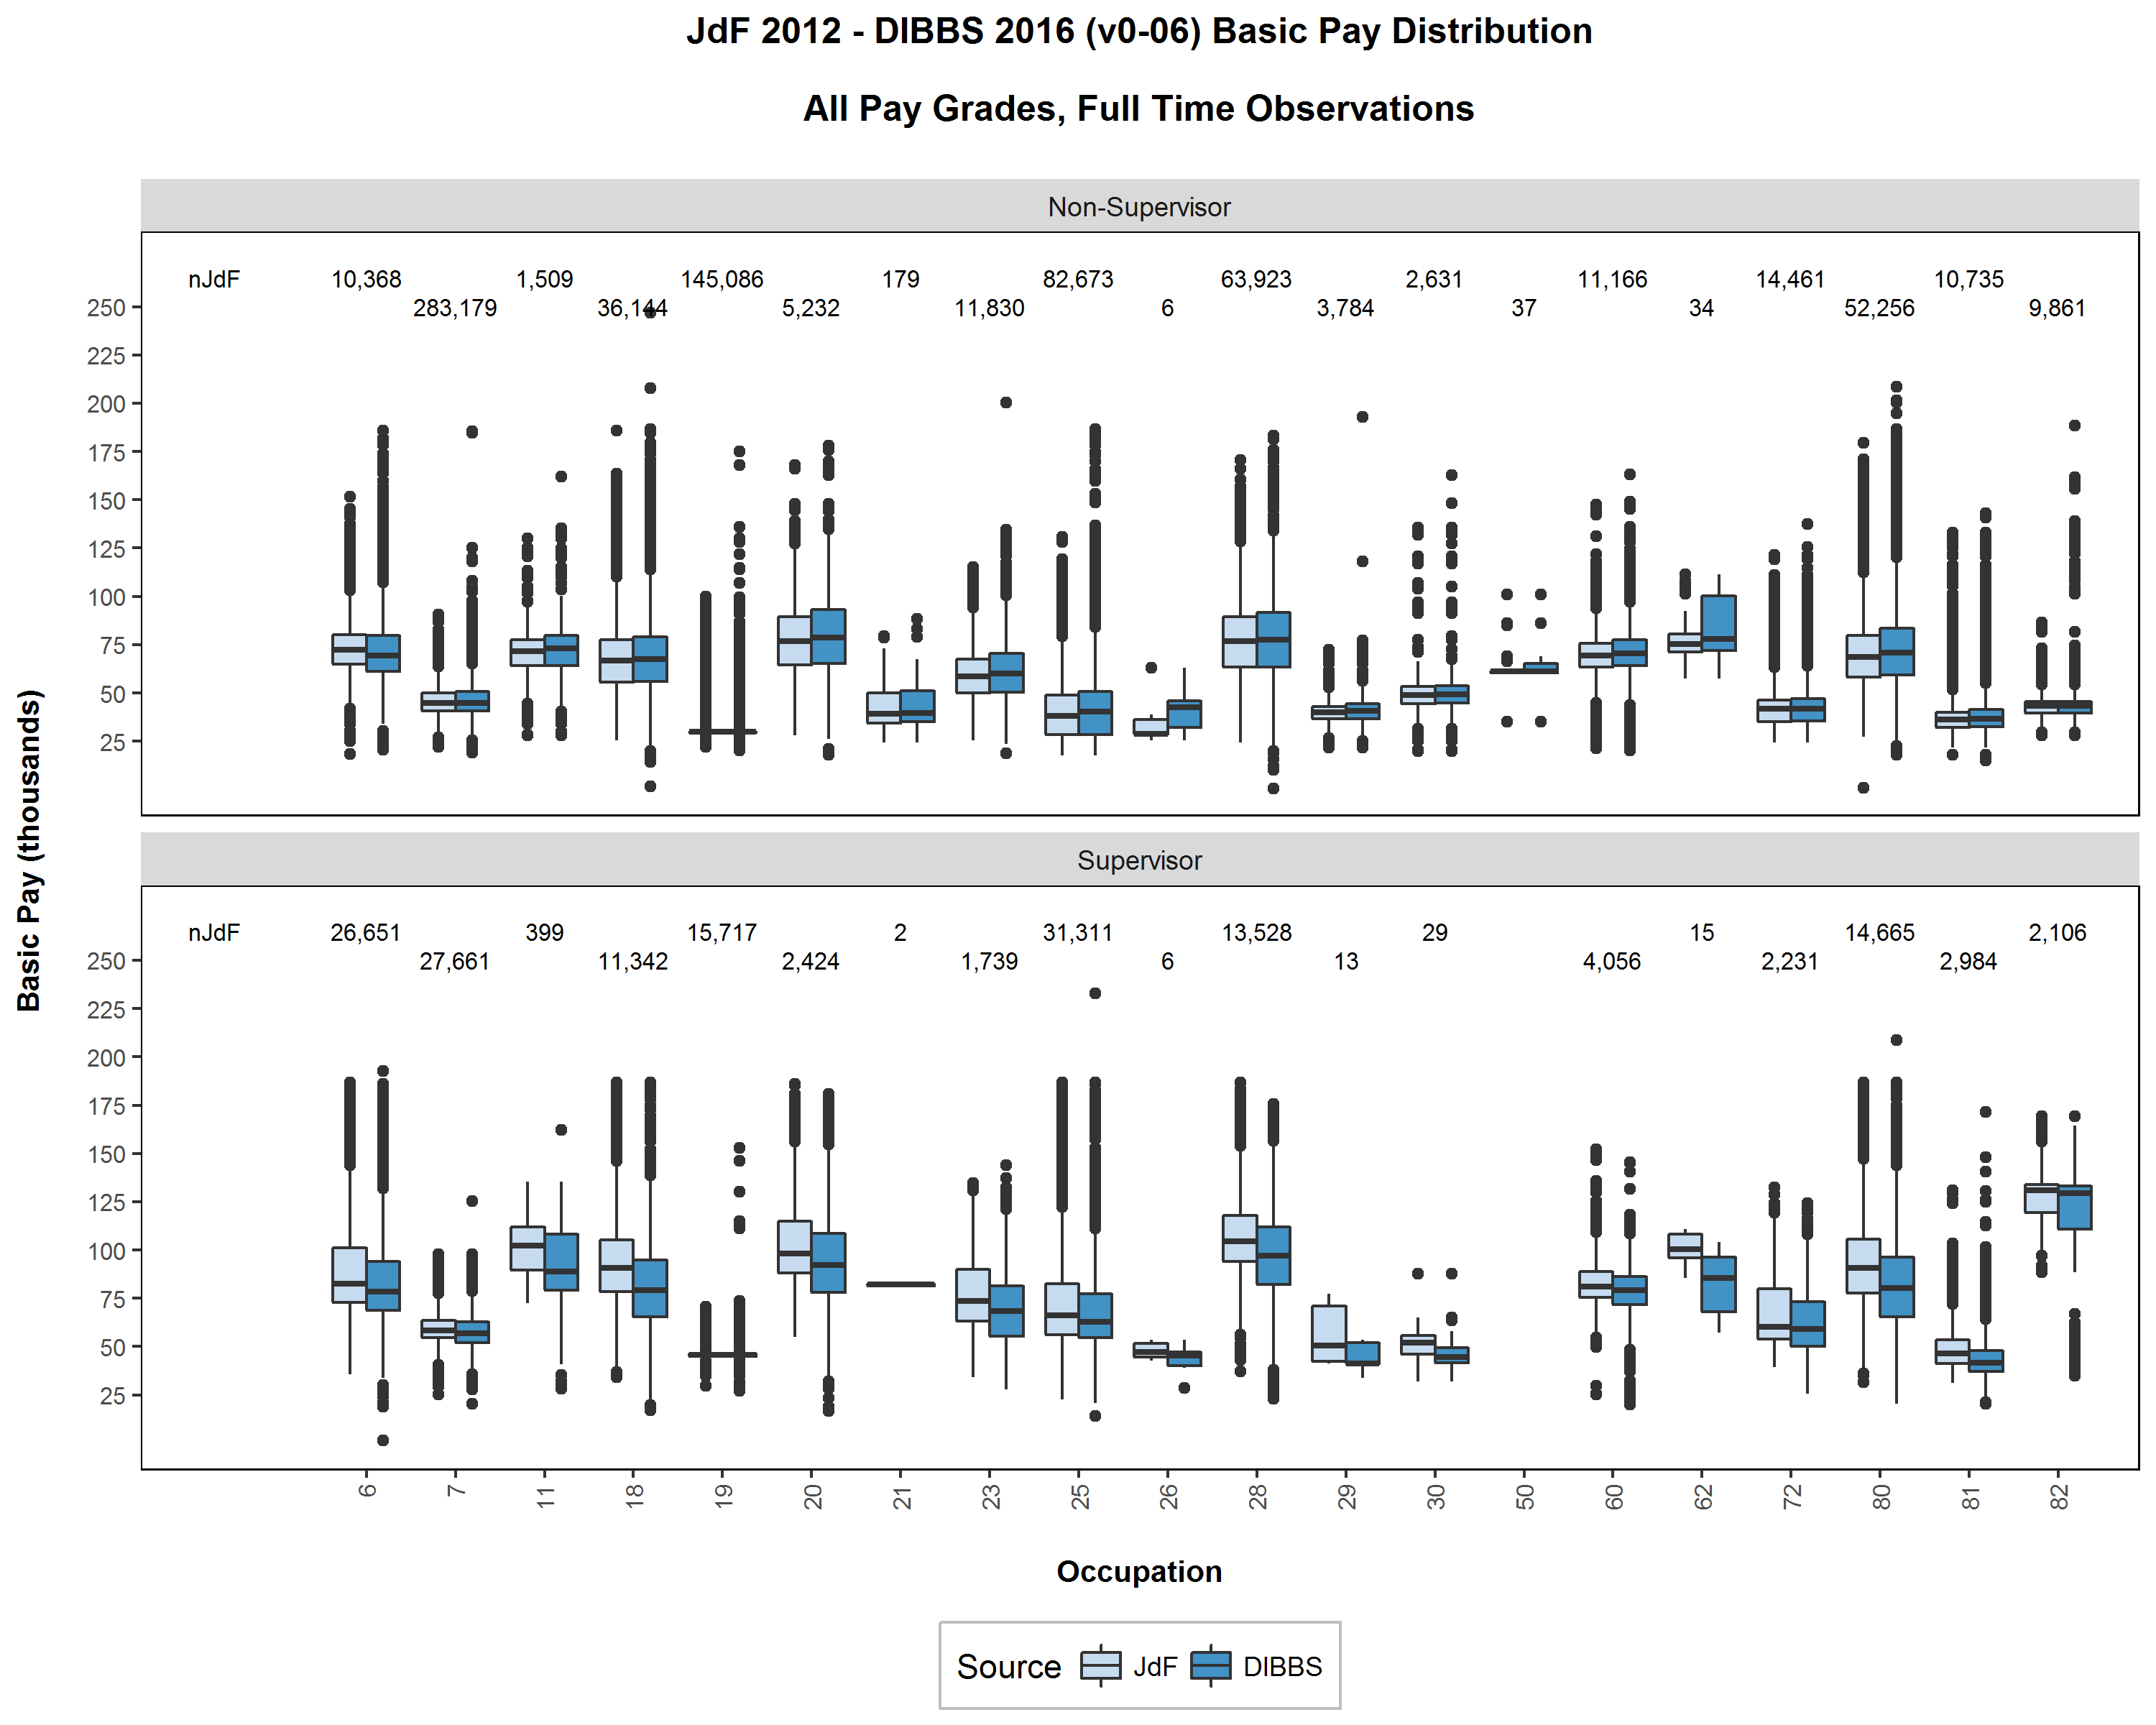
\includegraphics[width=6in, trim={0 1in 0 0.75in}, clip]{JdFDIBBSBasicPaySupervisoryStatusOccupation1.png}
        \caption{Occupations 0006 through 0082}
        \vspace{10pt}
    \end{subfigure}
    \begin{subfigure}{1\textwidth}
        \centering
        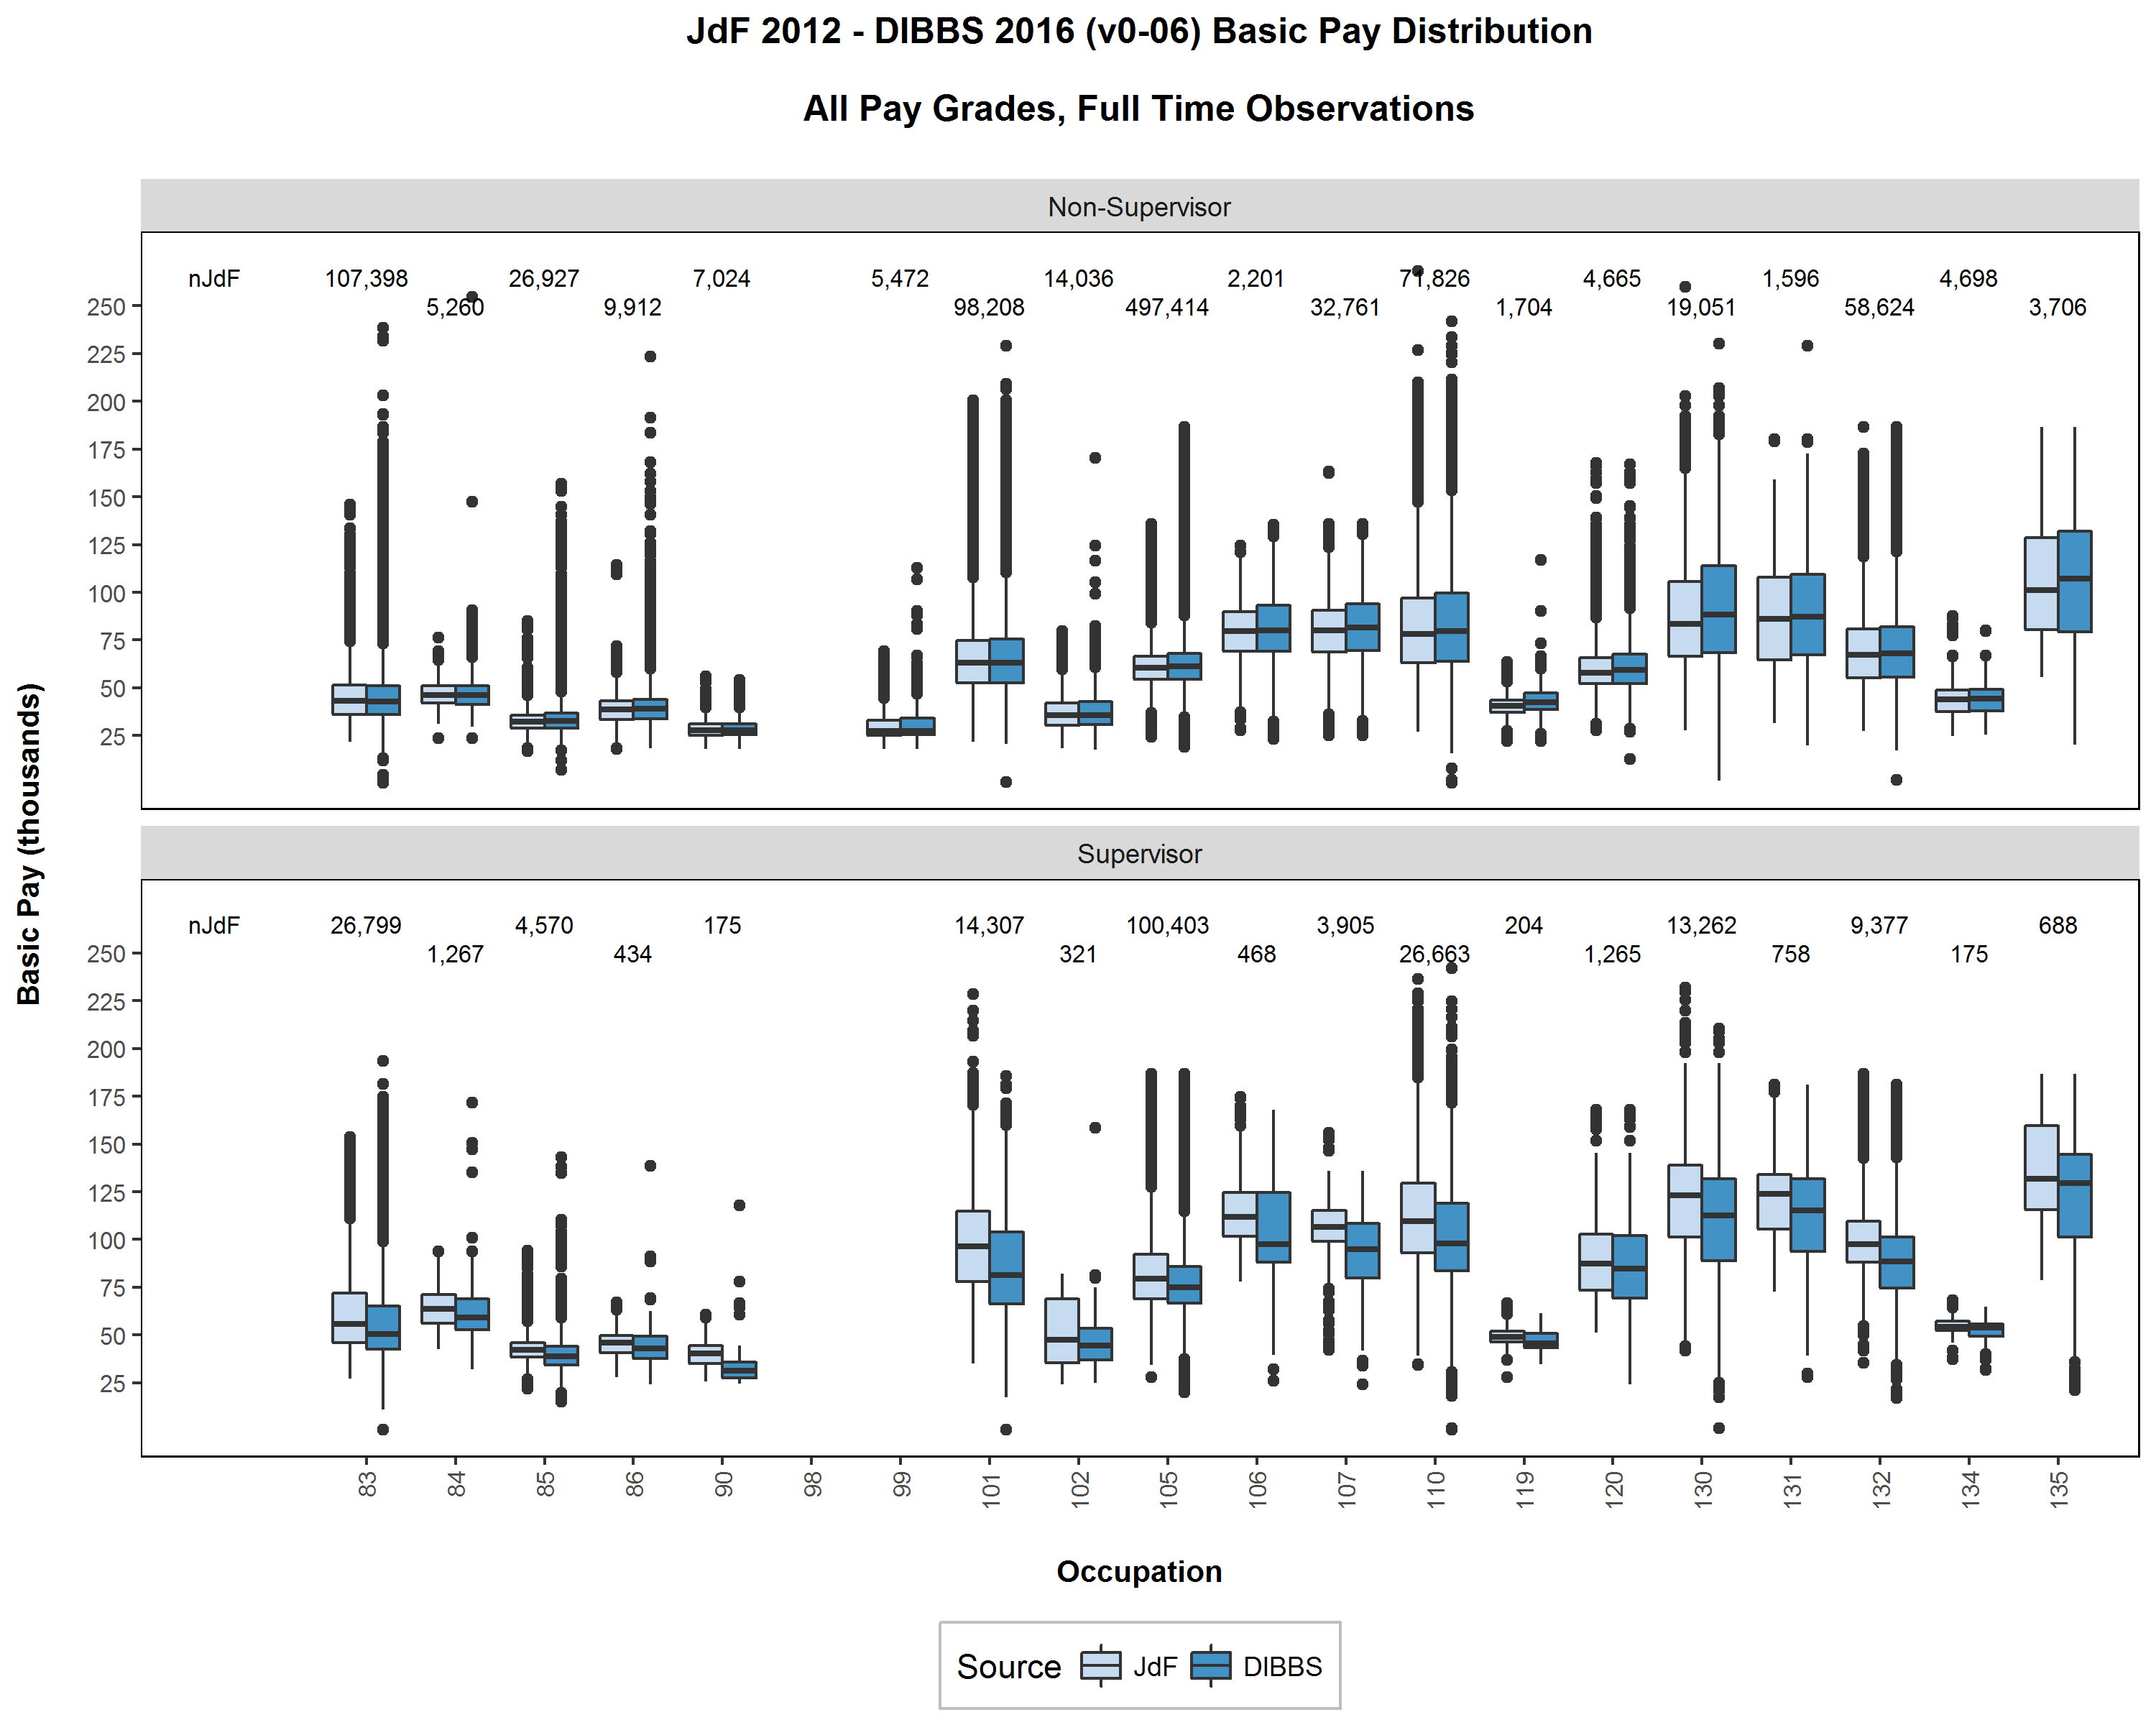
\includegraphics[width=6in, trim={0 1in 0 0.75in}, clip]{JdFDIBBSBasicPaySupervisoryStatusOccupation21.png}
        \caption{Occupations 0083 through 0135}
        \vspace{10pt}
    \end{subfigure}
    \caption{Basic pay distribution by occupation and supervisor status.  All agencies combined.  Authentic boxes on left, synthetic on right.  Occupation on x-axis.}
    \label{figure:JdFDIBBSBasicPaySupervisoryStatusOccupation1}
\end{figure}

\clearpage

\begin{figure}[h]
    \centering
    \begin{subfigure}{1\textwidth}
        \centering
        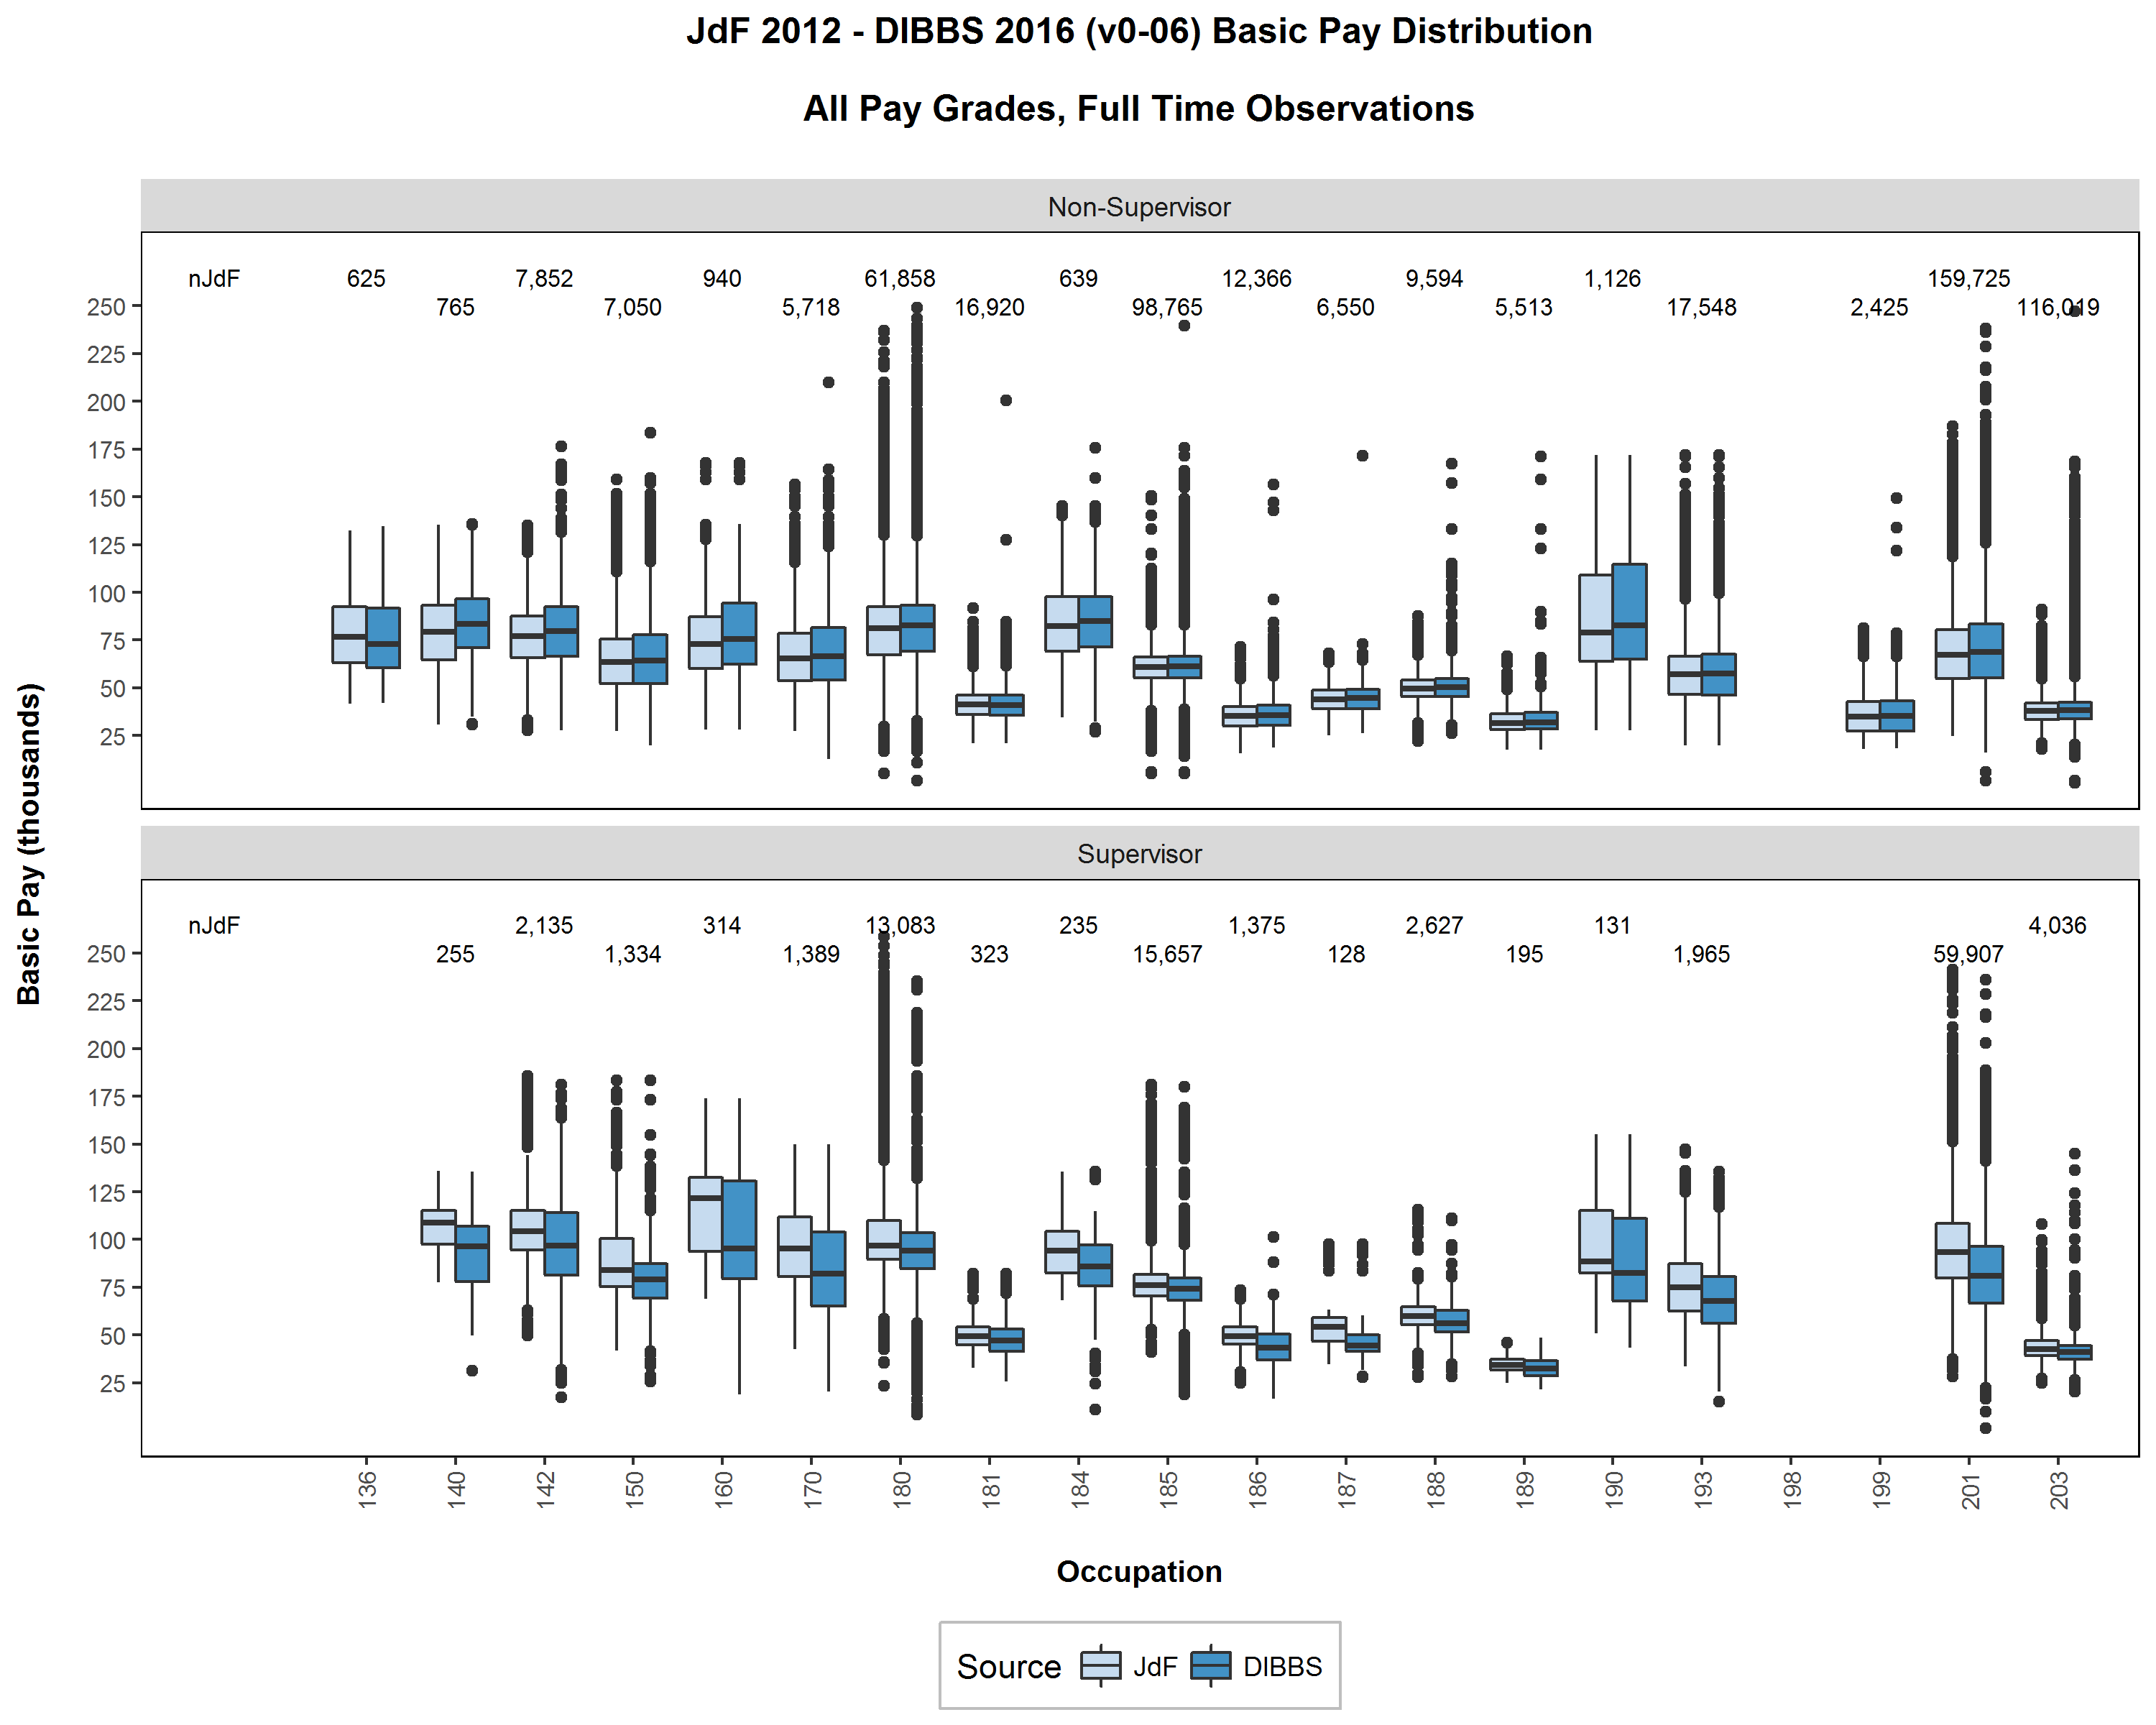
\includegraphics[width=6in, trim={0 1in 0 0.75in}, clip]{JdFDIBBSBasicPaySupervisoryStatusOccupation41.png}
        \caption{Occupations 0136 through 0203}
        \vspace{10pt}
    \end{subfigure}
    \begin{subfigure}{1\textwidth}
        \centering
        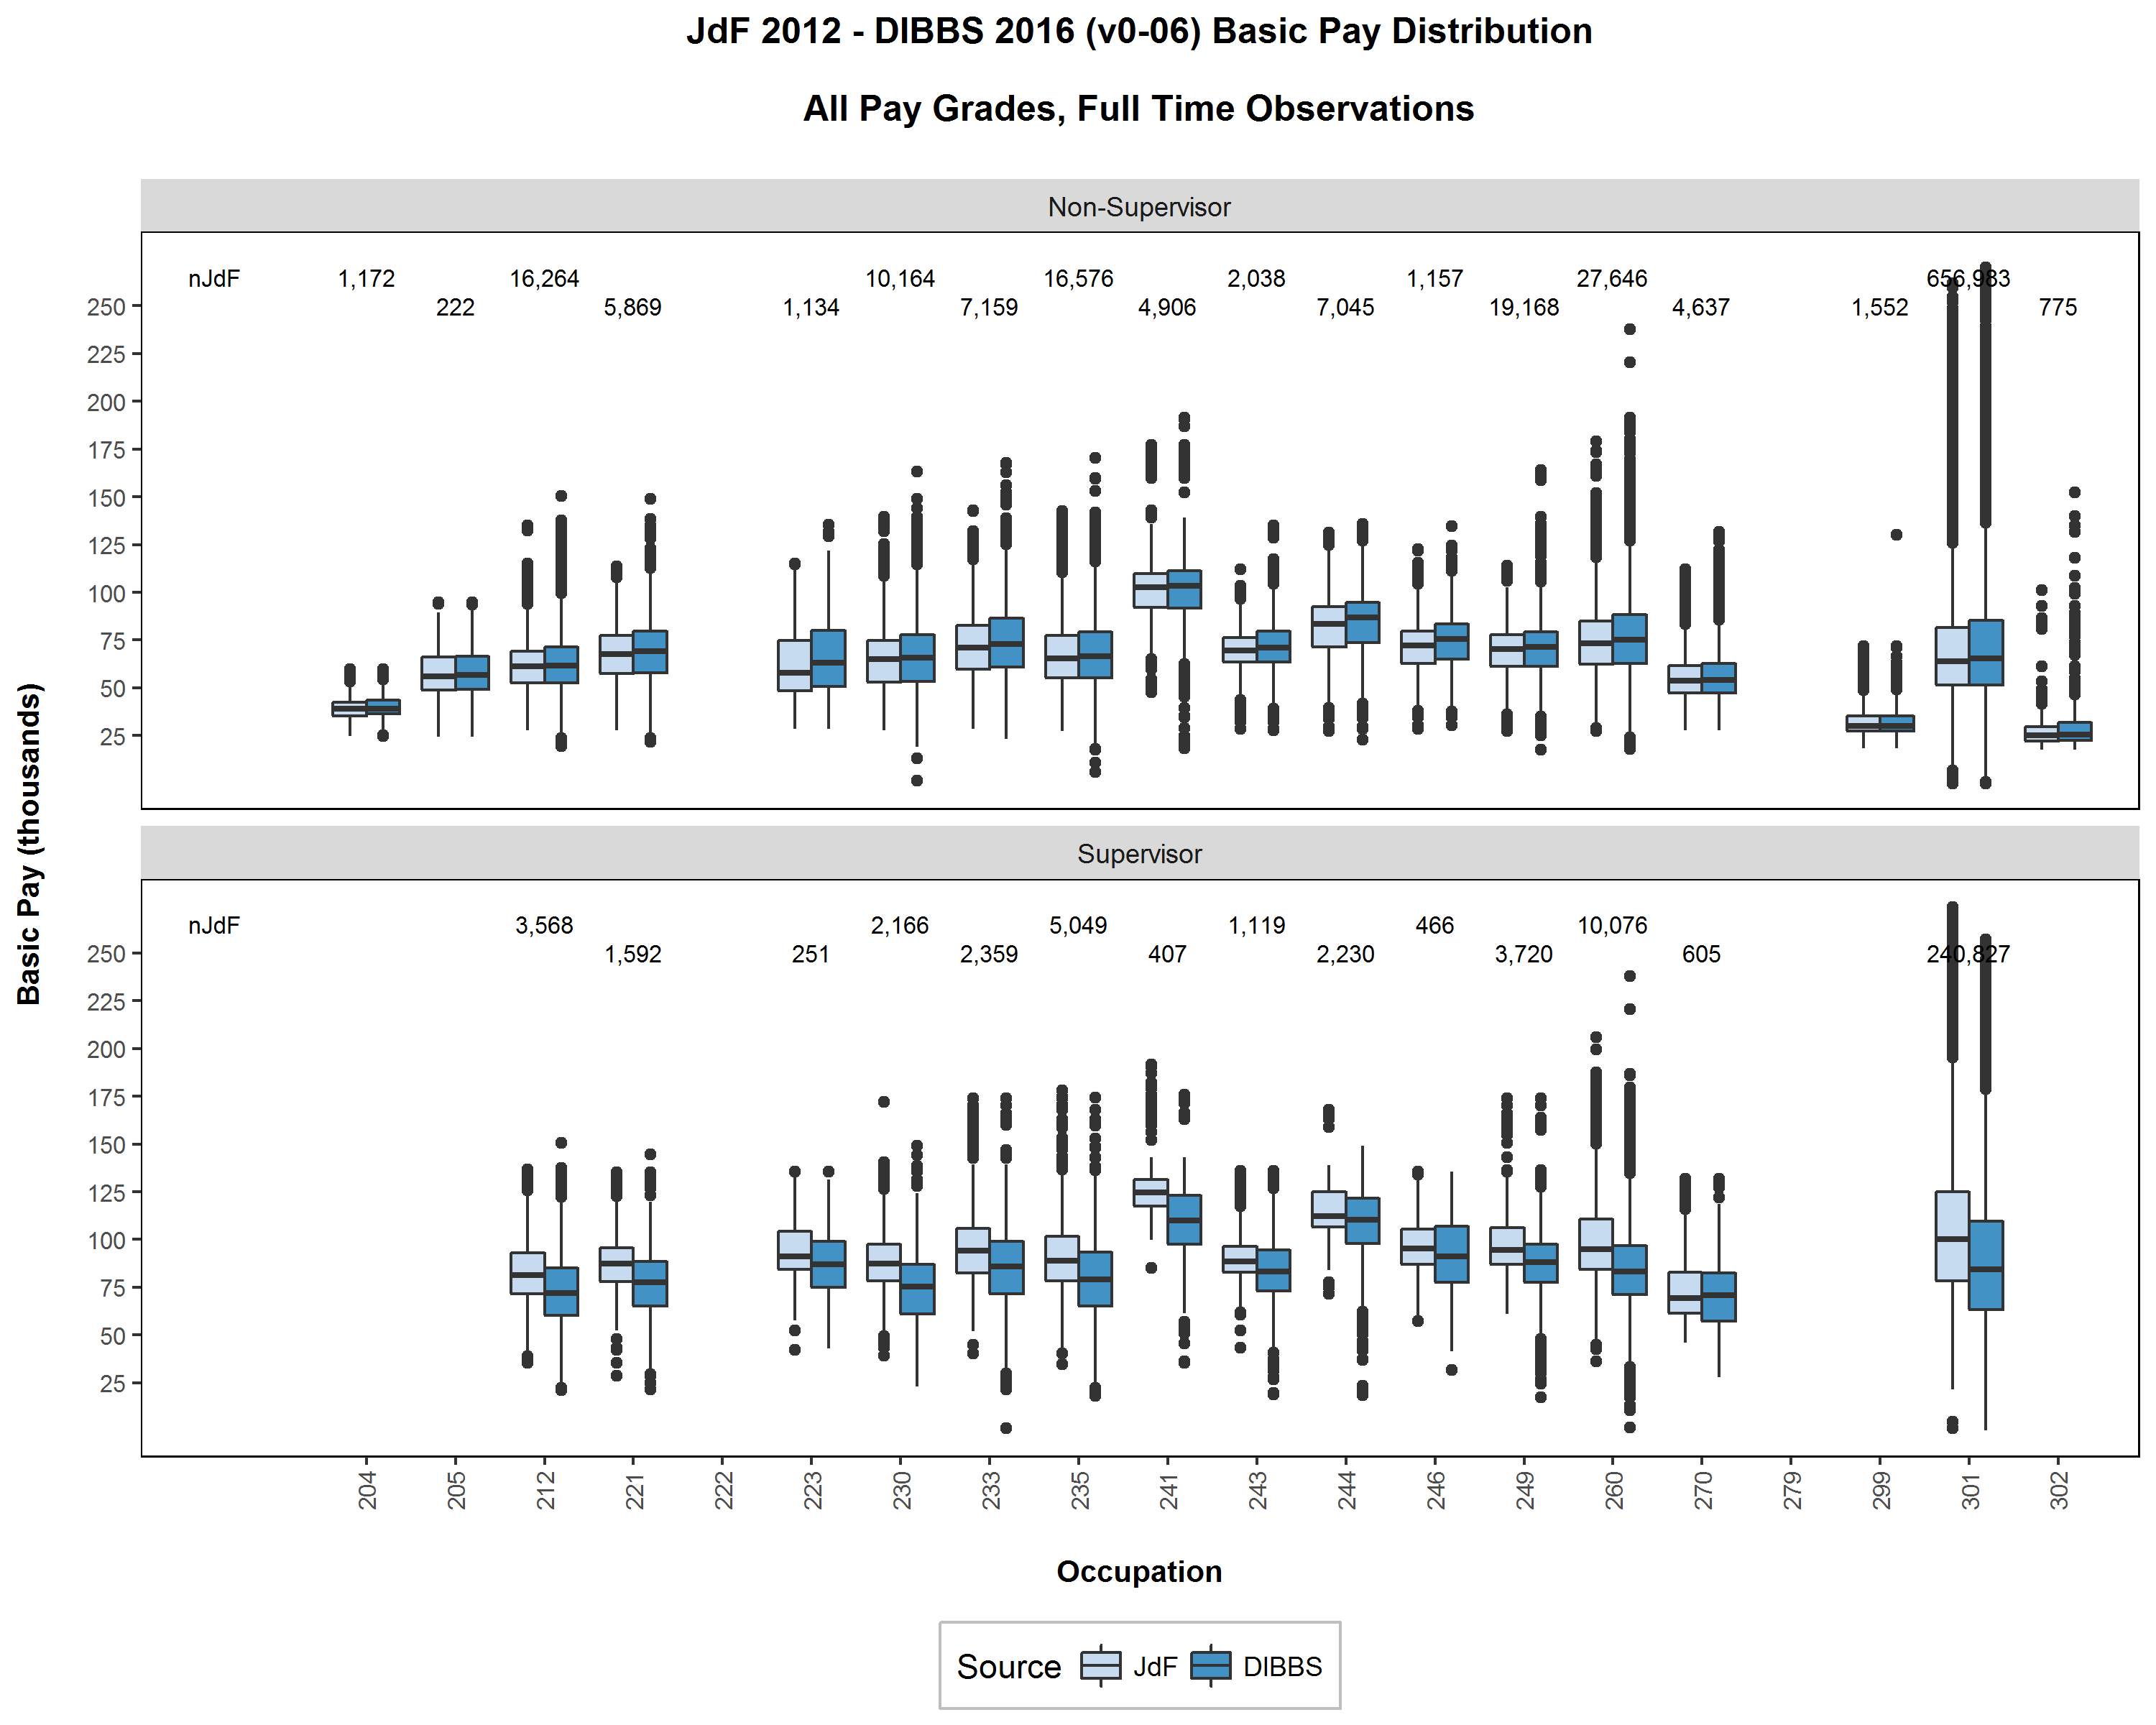
\includegraphics[width=6in, trim={0 1in 0 0.75in}, clip]{JdFDIBBSBasicPaySupervisoryStatusOccupation61.png}
        \caption{Occupations 0204 through 0302}
        \vspace{10pt}
    \end{subfigure}
    \caption{Basic pay distribution by occupation and supervisor status.  All agencies combined.  Authentic boxes on left, synthetic on right.  Occupation on x-axis.}
    \label{figure:JdFDIBBSBasicPaySupervisoryStatusOccupation2}
\end{figure}

\clearpage

\begin{figure}[h]
    \centering
    \begin{subfigure}{1\textwidth}
        \centering
        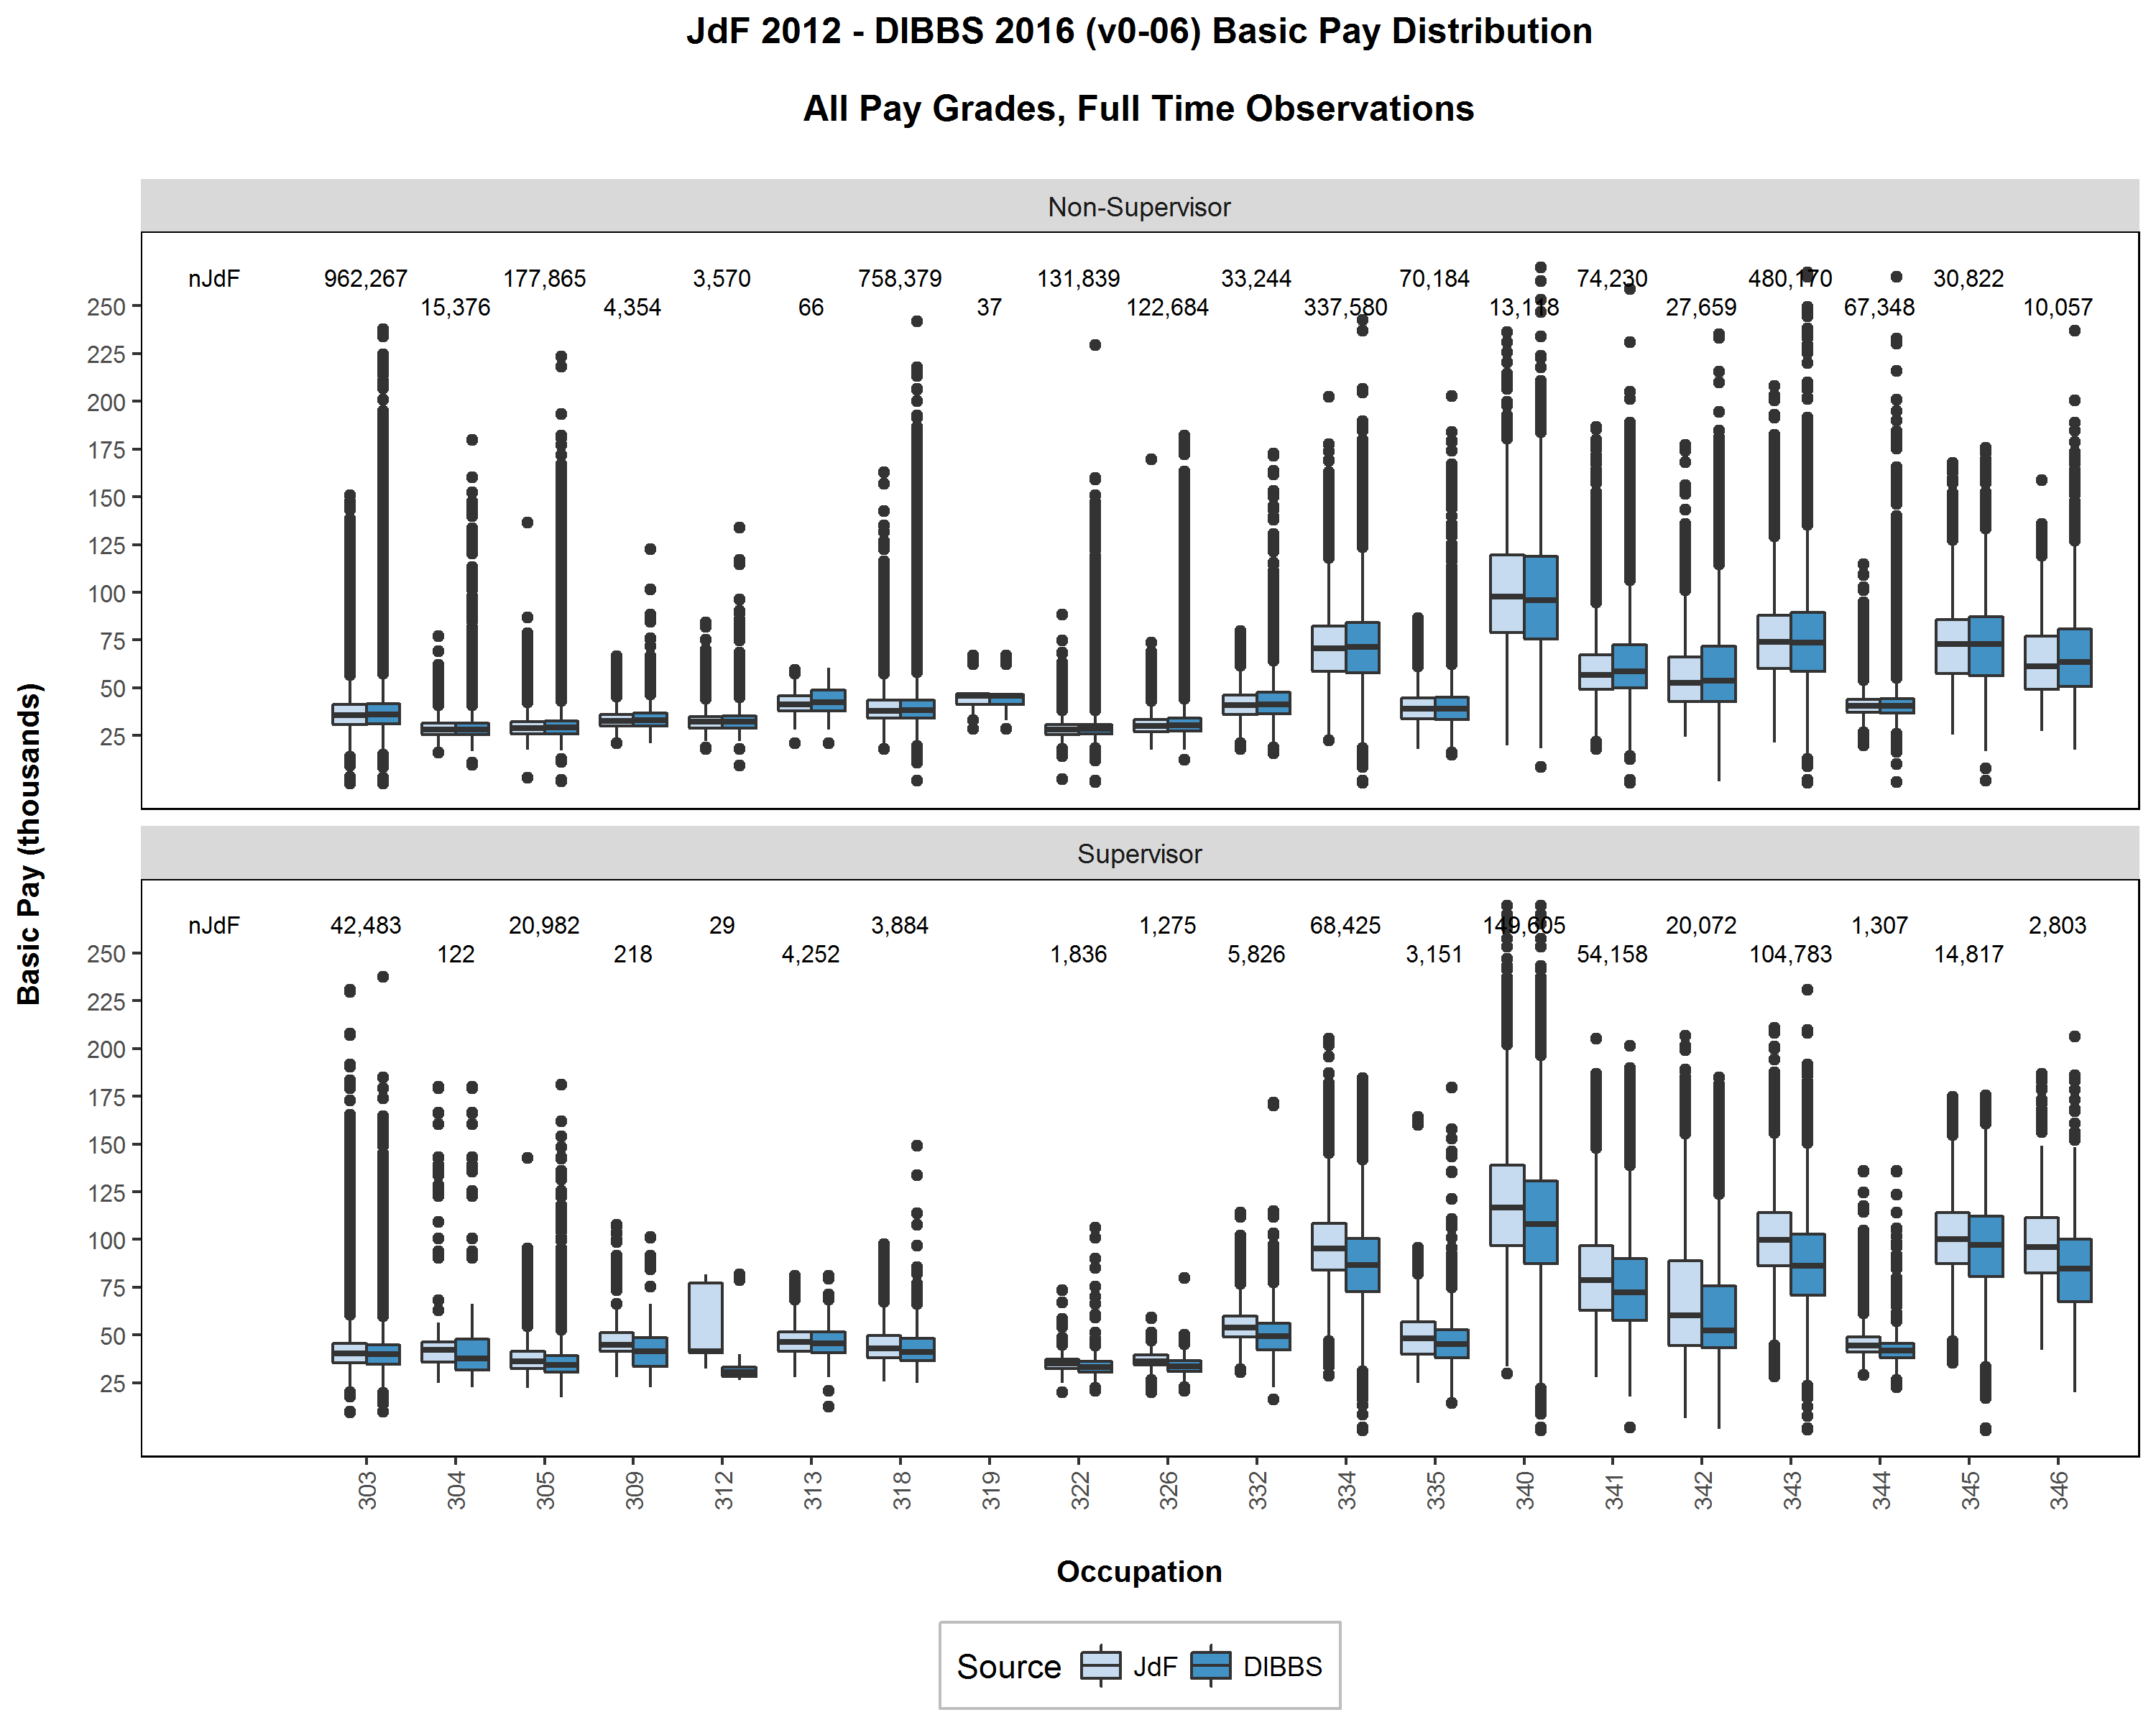
\includegraphics[width=6in, trim={0 1in 0 0.75in}, clip]{JdFDIBBSBasicPaySupervisoryStatusOccupation81.png}
        \caption{Occupations 0303 through 0346}
        \vspace{10pt}
    \end{subfigure}
    \begin{subfigure}{1\textwidth}
        \centering
        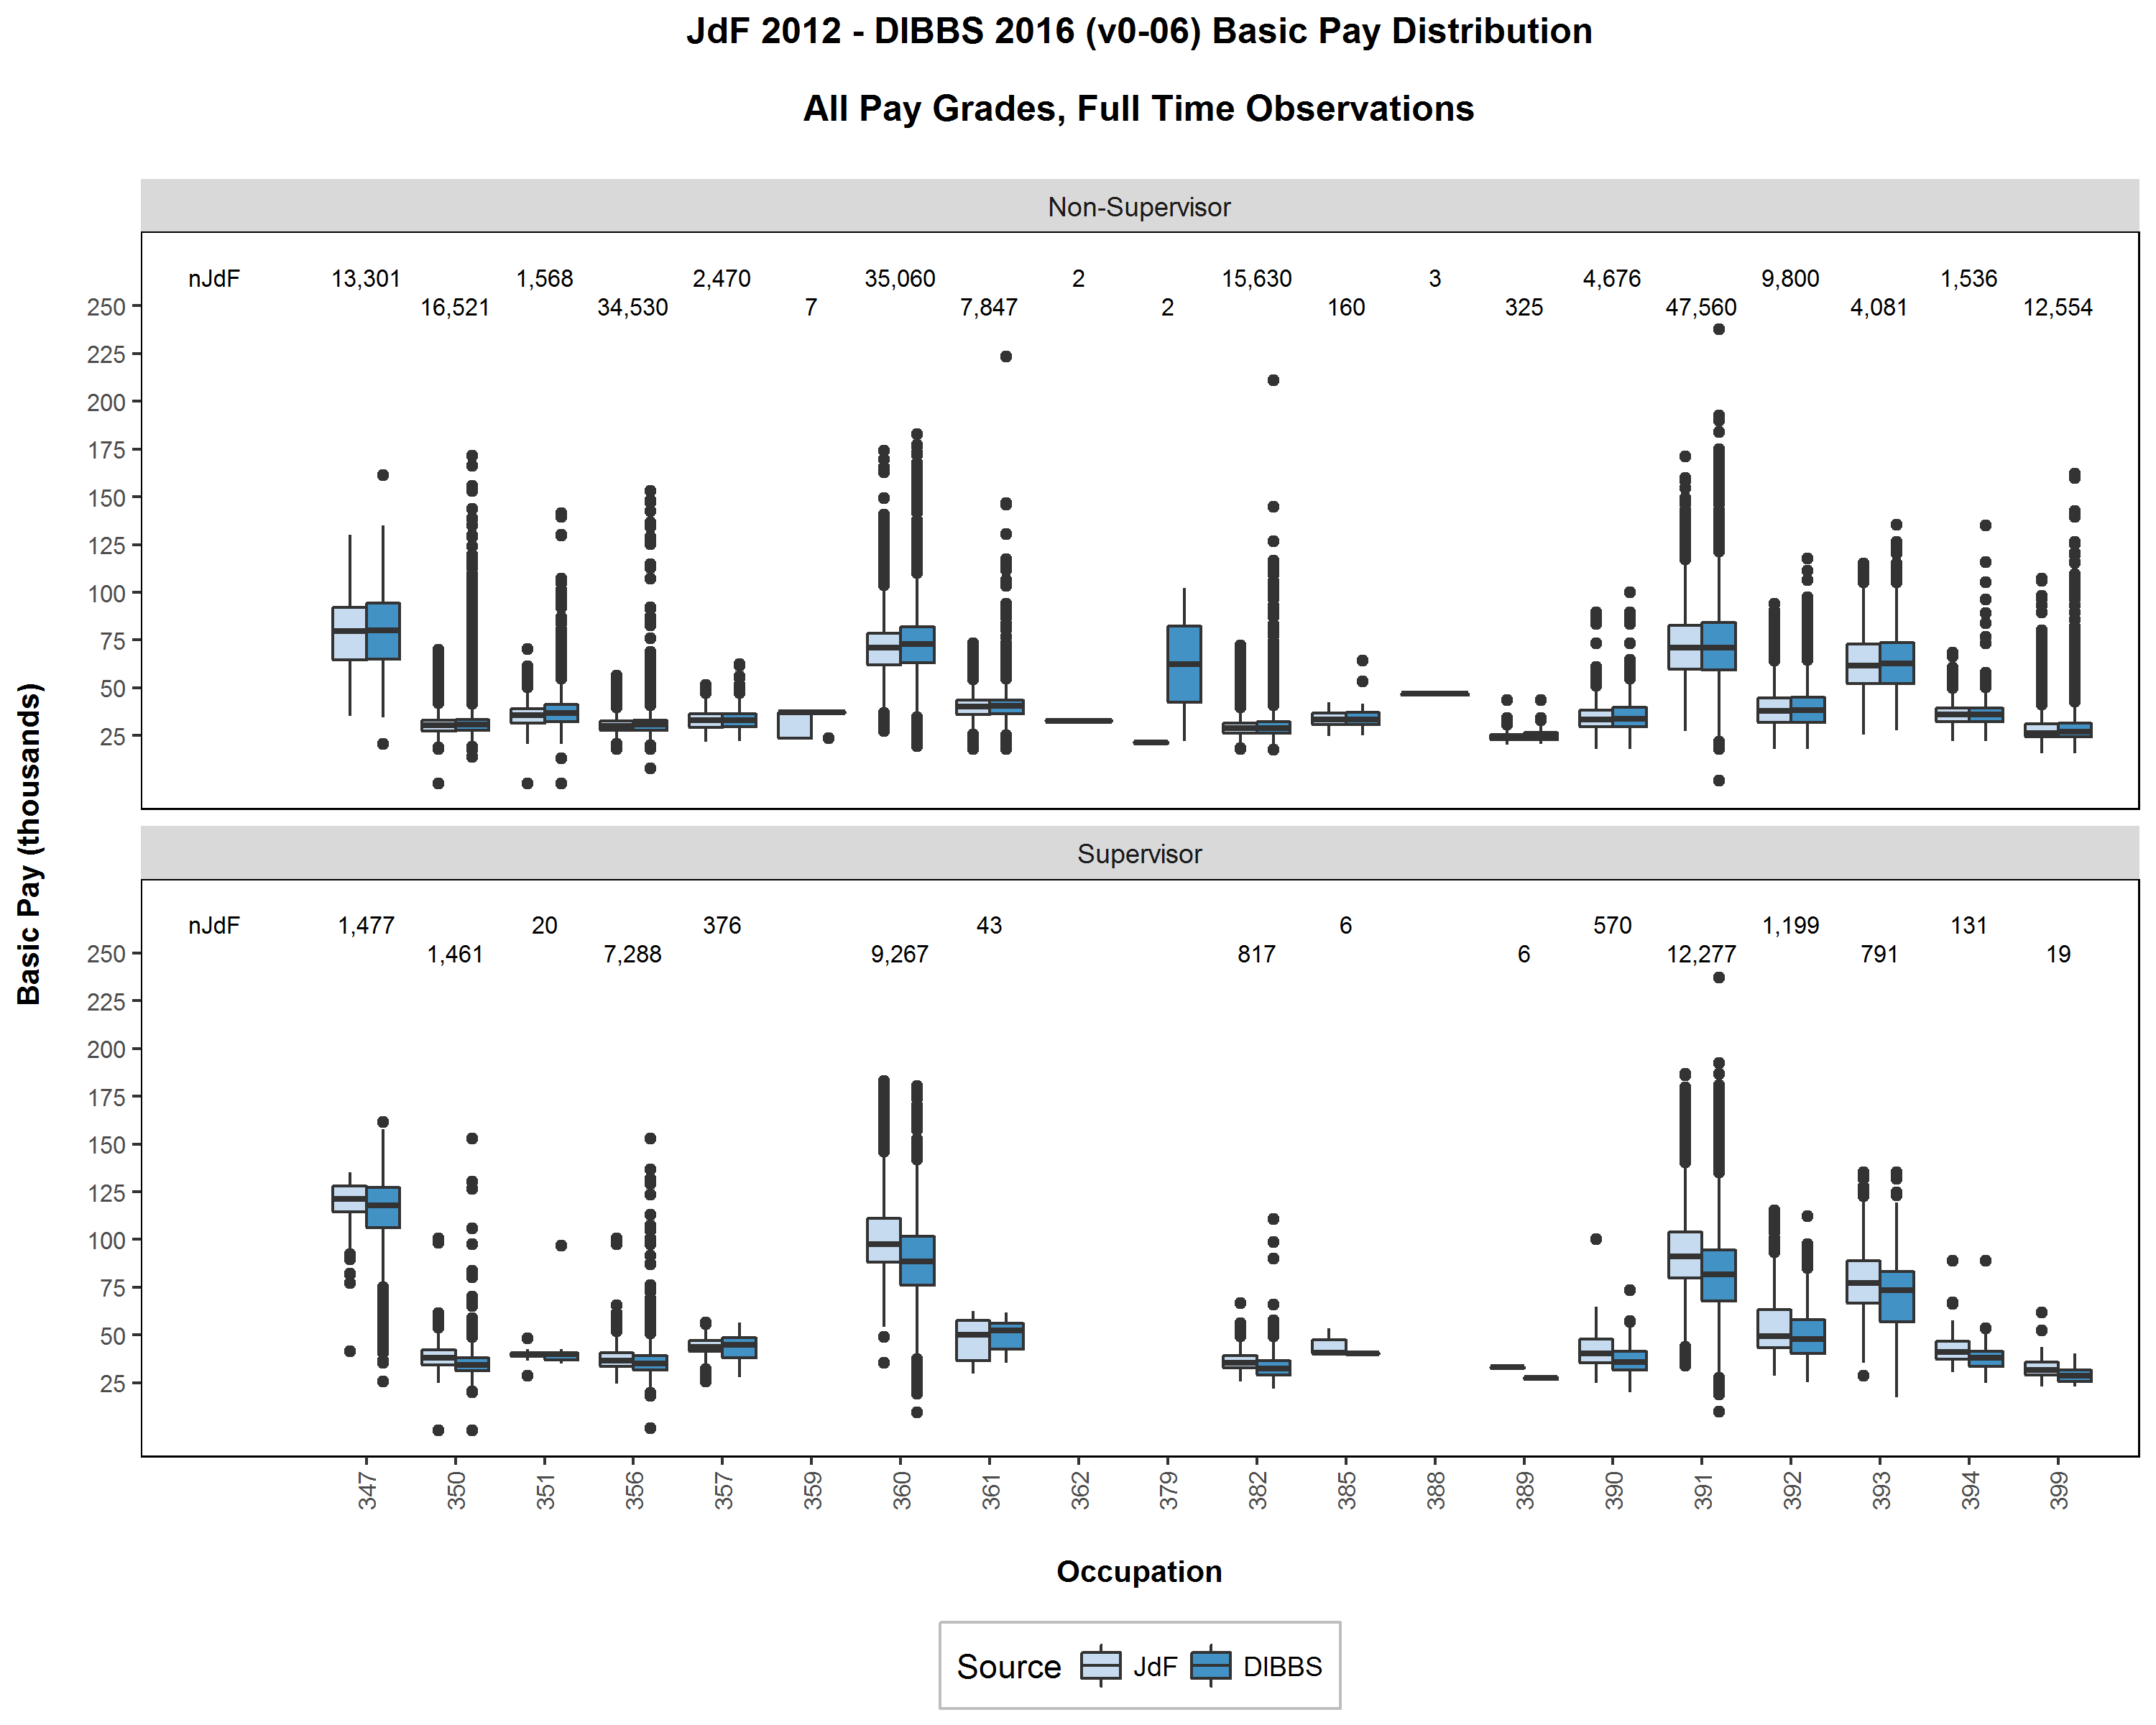
\includegraphics[width=6in, trim={0 1in 0 0.75in}, clip]{JdFDIBBSBasicPaySupervisoryStatusOccupation101.png}
        \caption{Occupations 0347 through 0399}
        \vspace{10pt}
    \end{subfigure}
    \caption{Basic pay distribution by occupation and supervisor status.  All agencies combined.  Authentic boxes on left, synthetic on right.  Occupation on x-axis.}
    \label{figure:JdFDIBBSBasicPaySupervisoryStatusOccupation3}
\end{figure}

\begin{figure}[h]
    \centering
    \begin{subfigure}{1\textwidth}
        \centering
        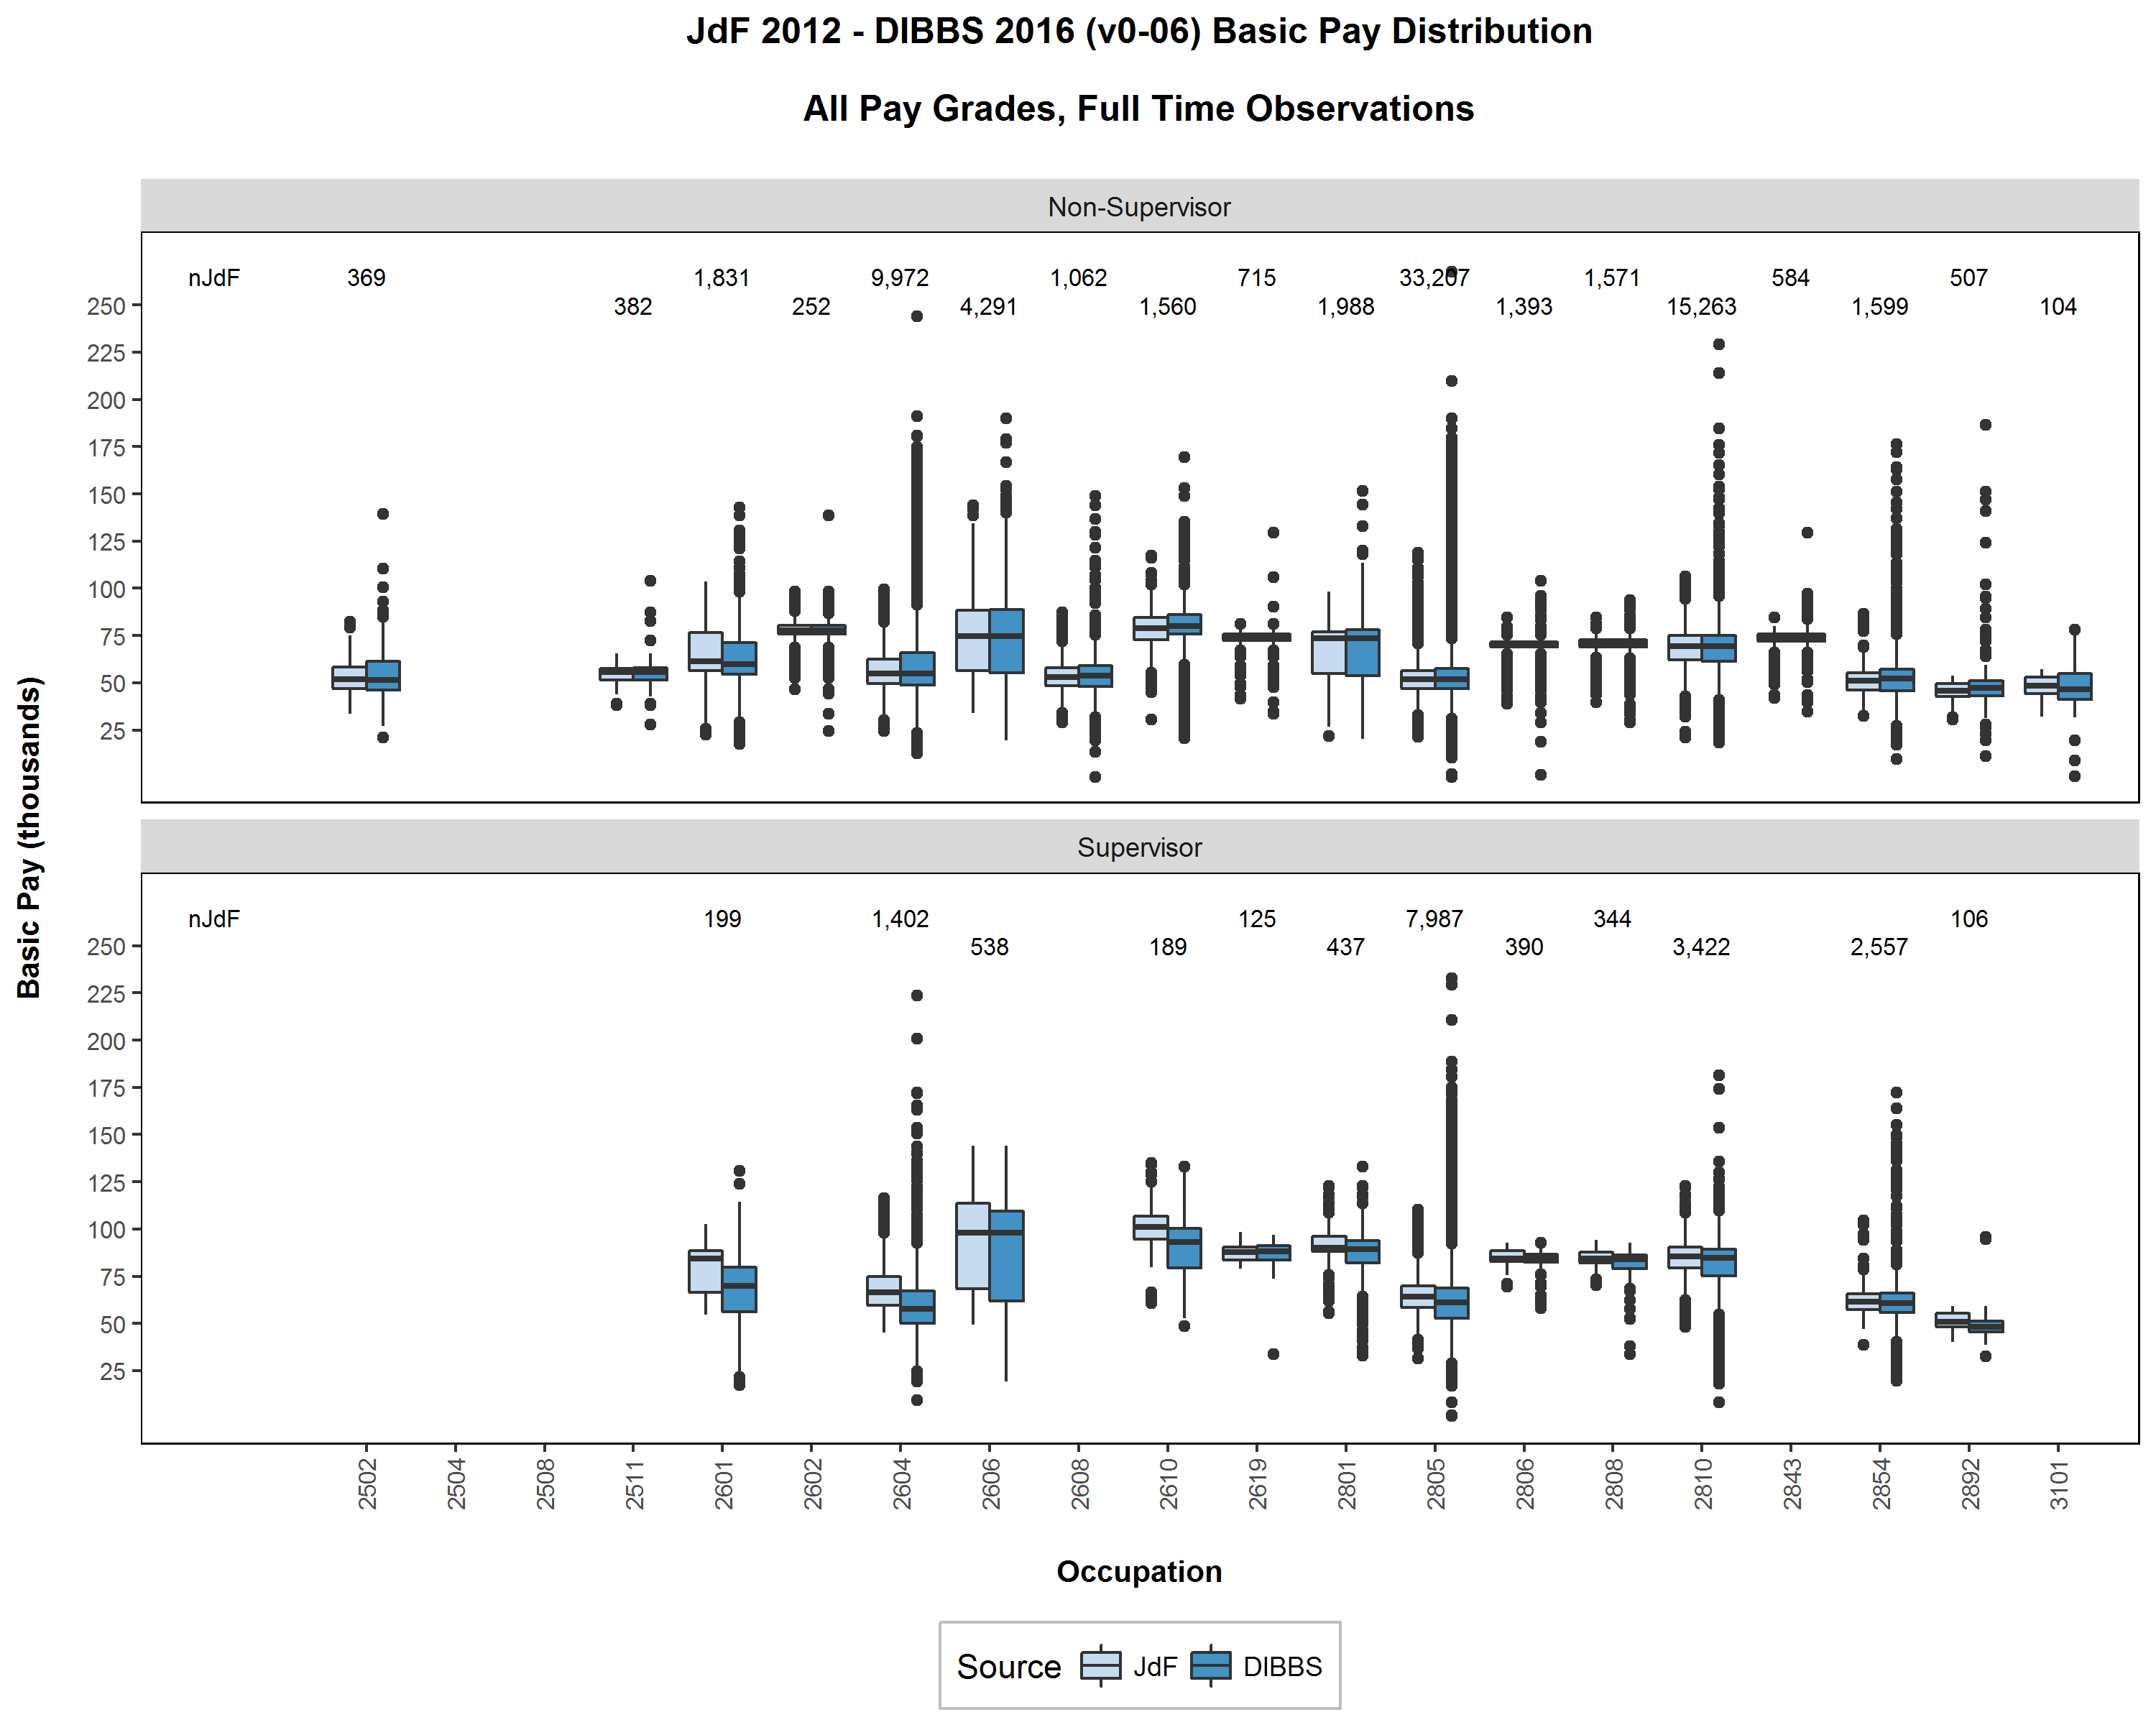
\includegraphics[width=6in, trim={0 1in 0 0.75in}, clip]{JdFDIBBSBasicPaySupervisoryStatusOccupation481.png}
        \caption{Occupations 2502 through 3101 (trades)}
        \vspace{10pt}
    \end{subfigure}
    \begin{subfigure}{1\textwidth}
        \centering
        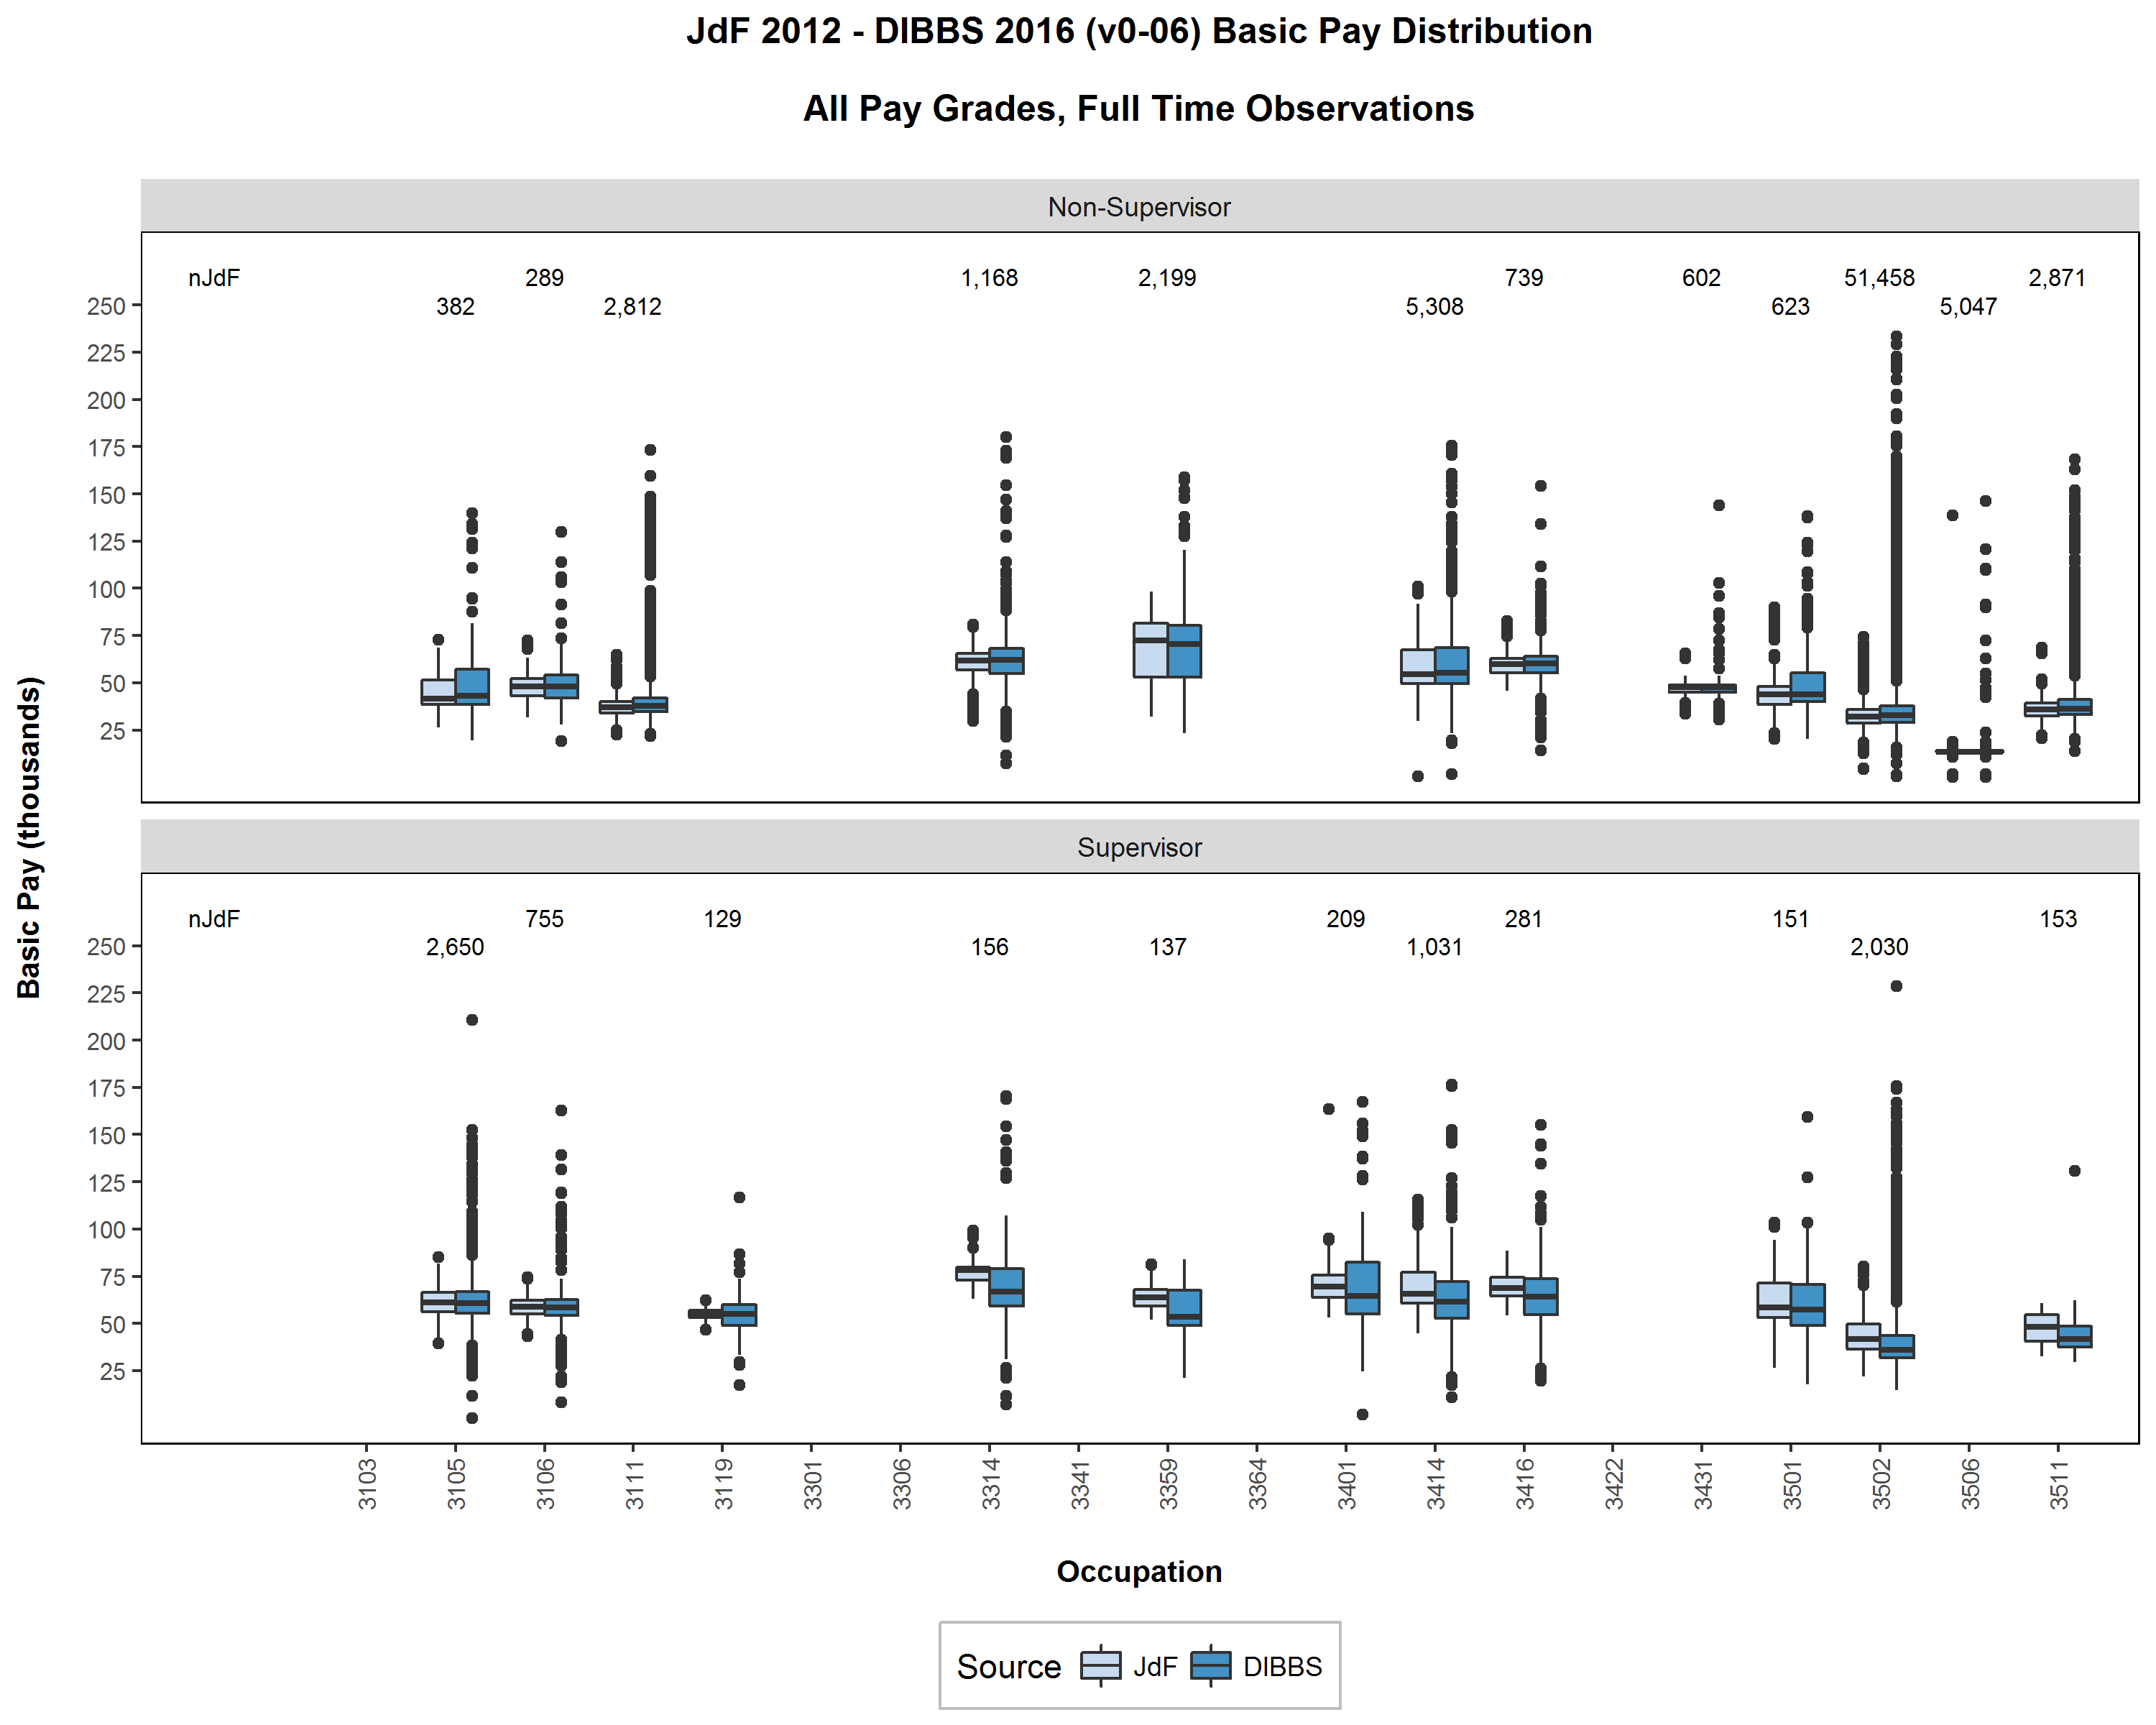
\includegraphics[width=6in, trim={0 1in 0 0.75in}, clip]{JdFDIBBSBasicPaySupervisoryStatusOccupation501.png}
        \caption{Occupations 3103 through 3511 (trades)}
        \vspace{10pt}
    \end{subfigure}
    \caption{Basic pay distribution by occupation and supervisor status.  All agencies combined.  Authentic boxes on left, synthetic on right.  Occupation on x-axis.}
    \label{figure:JdFDIBBSBasicPaySupervisoryStatusOccupation4}
\end{figure}

\clearpage

\begin{figure}[h]
    \centering
    \begin{subfigure}{1\textwidth}
        \centering
        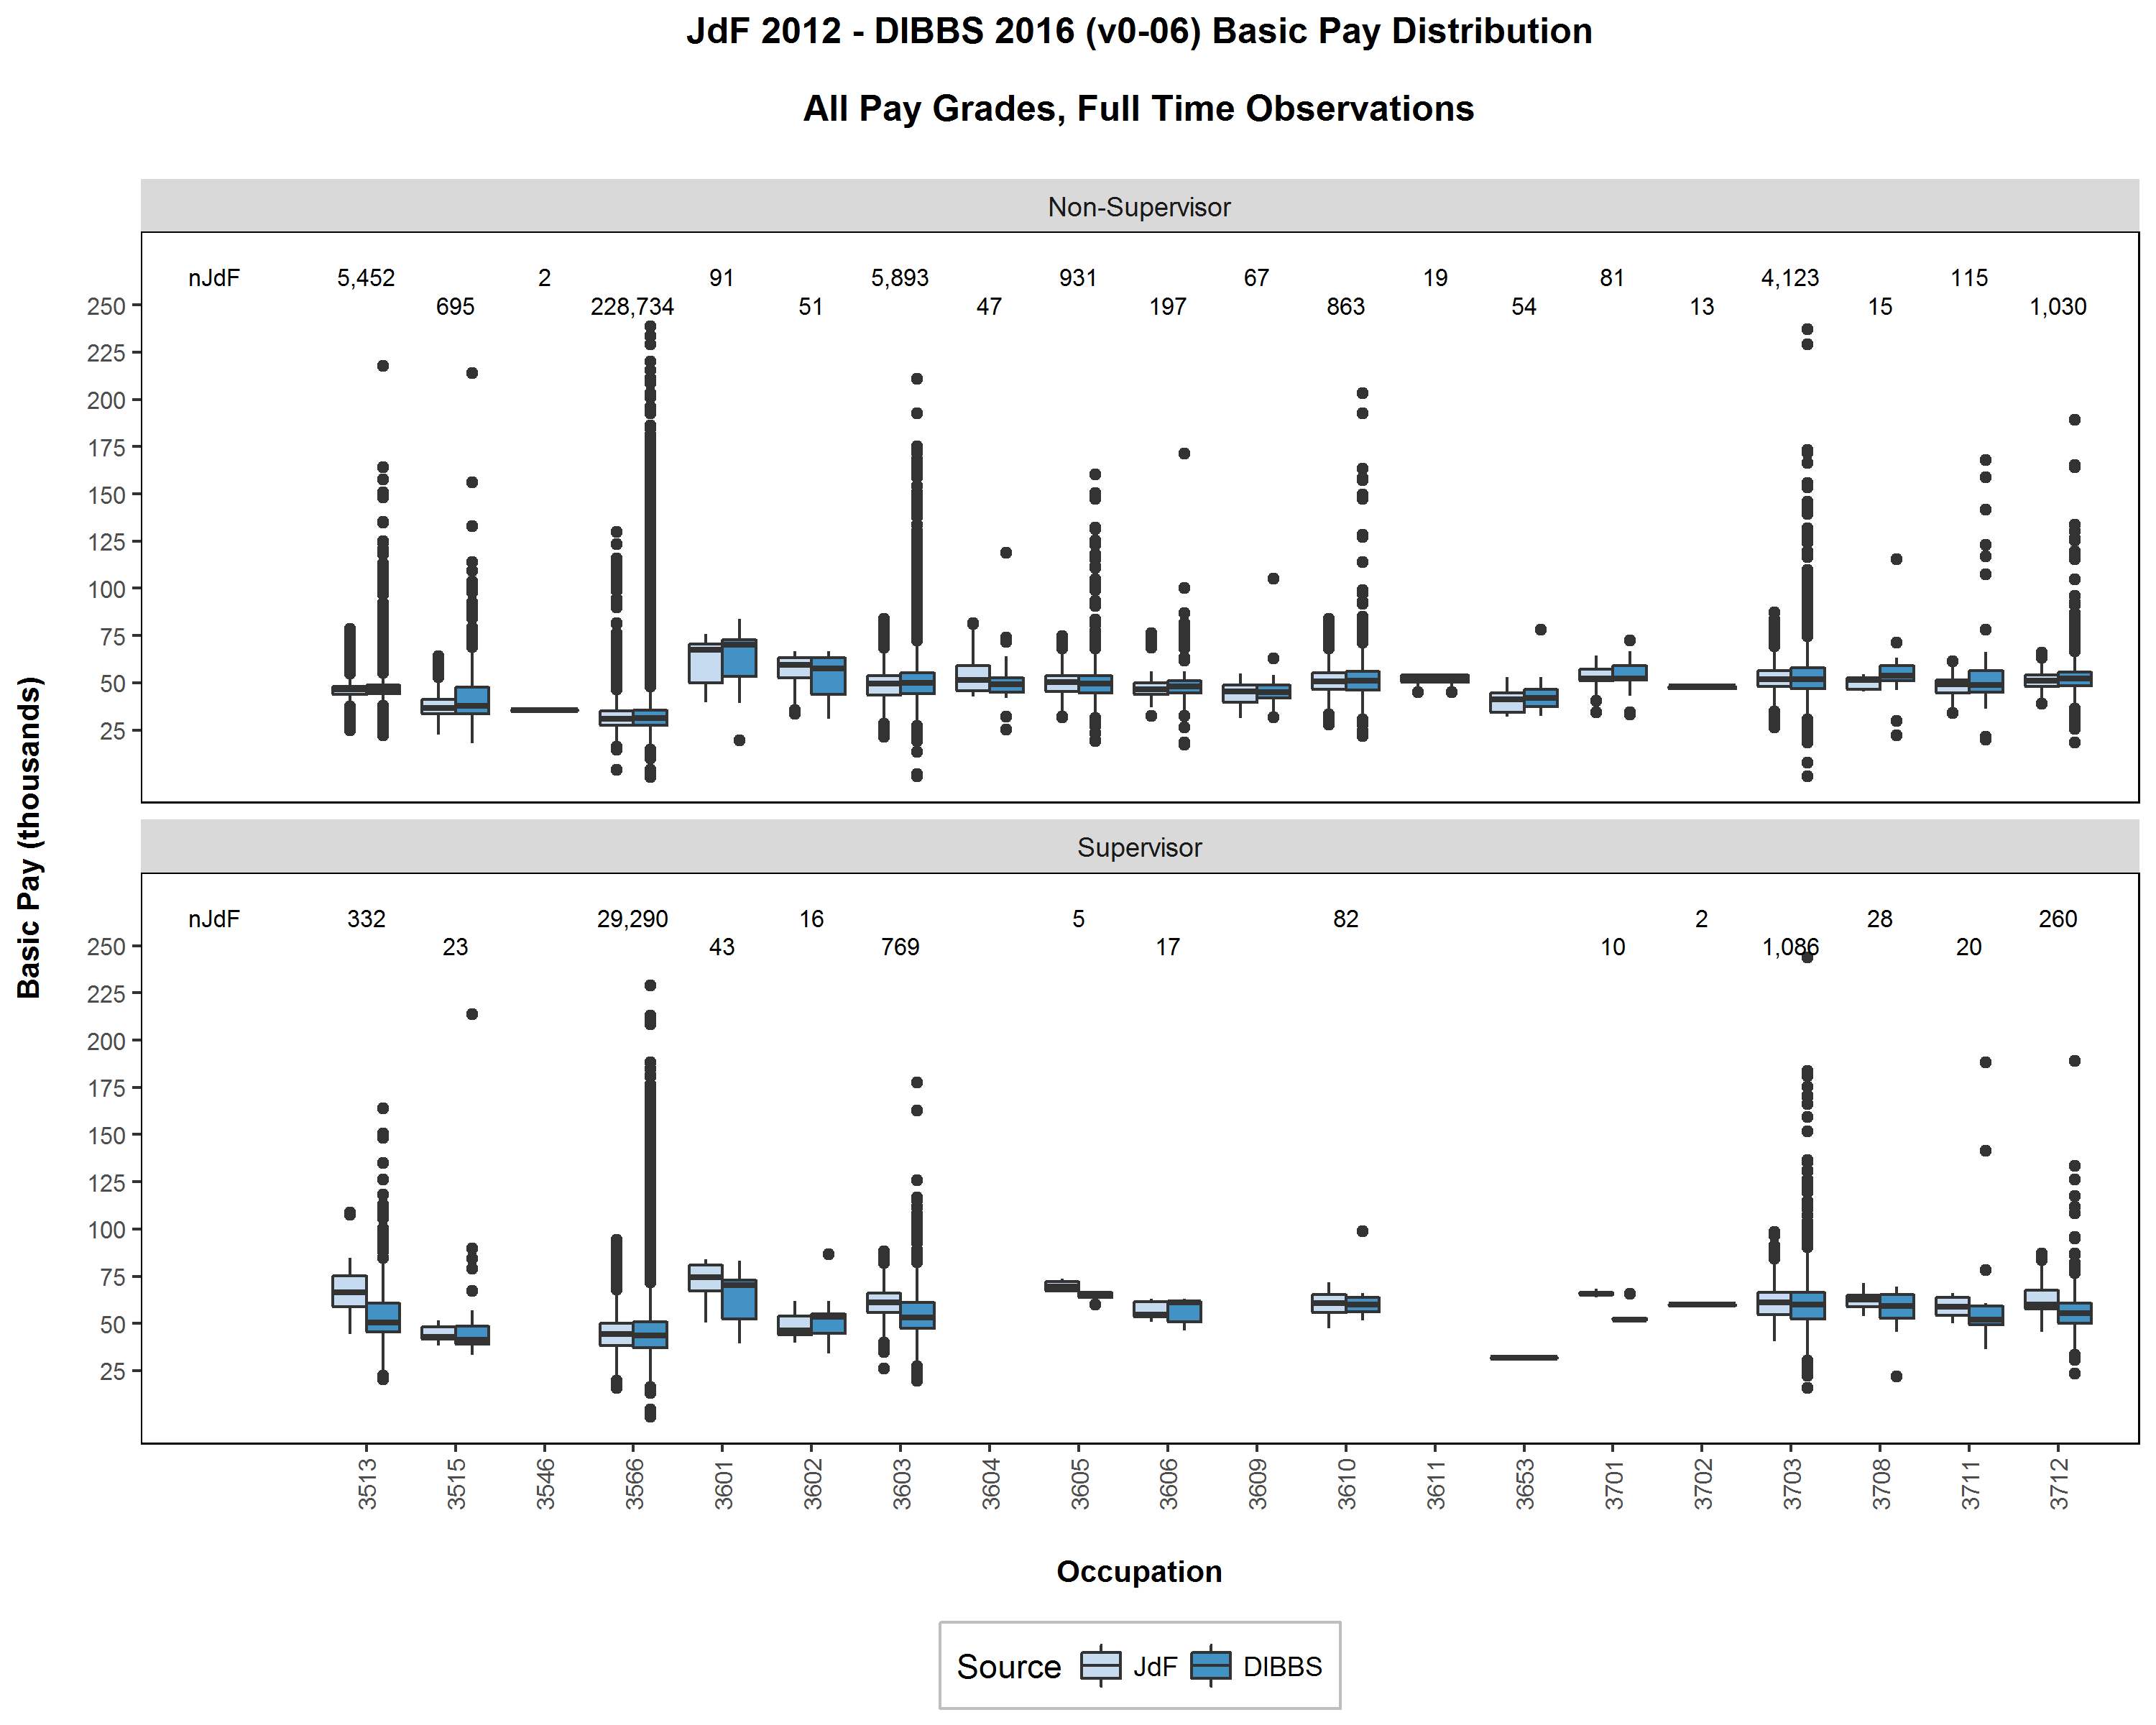
\includegraphics[width=6in, trim={0 1in 0 0.75in}, clip]{JdFDIBBSBasicPaySupervisoryStatusOccupation521.png}
        \caption{Occupations 3513 through 3712 (trades)}
        \vspace{10pt}
    \end{subfigure}
    \begin{subfigure}{1\textwidth}
        \centering
        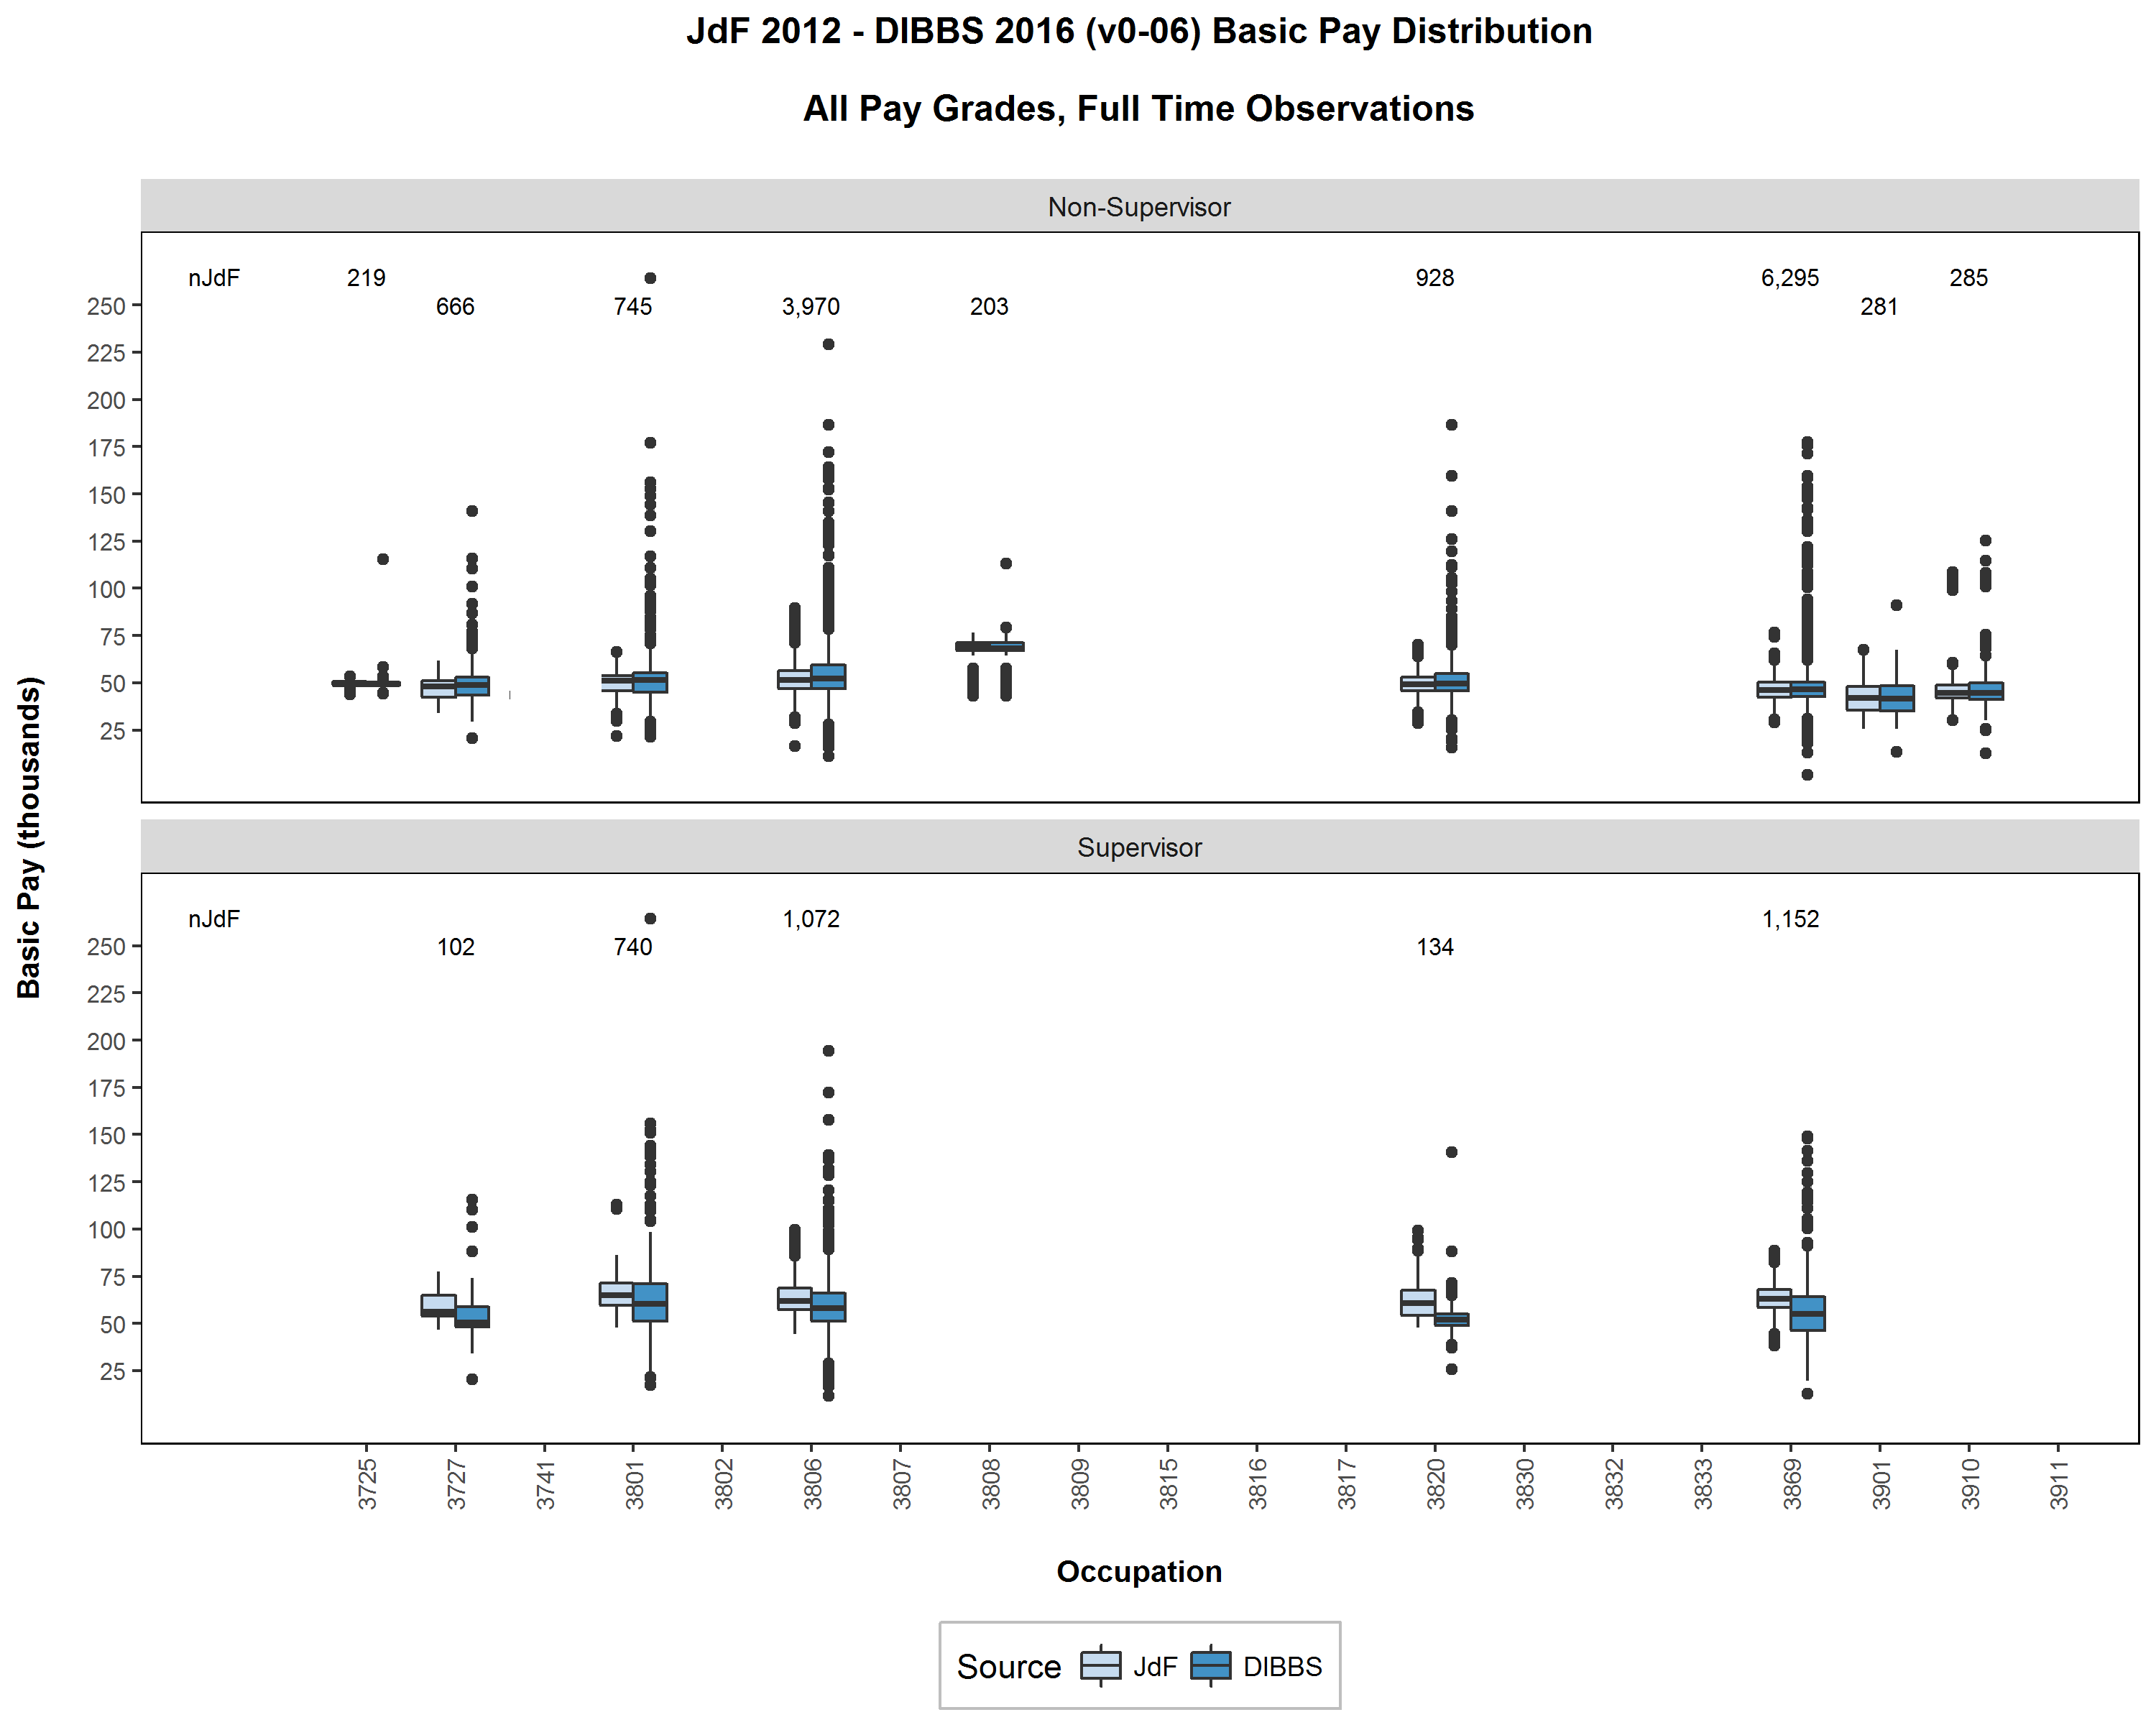
\includegraphics[width=6in, trim={0 1in 0 0.75in}, clip]{JdFDIBBSBasicPaySupervisoryStatusOccupation541.png}
        \caption{Occupations 3725 through 3911 (trades}
        \vspace{10pt}
    \end{subfigure}
    \caption{Basic pay distribution by occupation and supervisor status.  All agencies combined.  Authentic boxes on left, synthetic on right.  Occupation on x-axis.}
    \label{figure:JdFDIBBSBasicPaySupervisoryStatusOccupation5}
\end{figure}

\clearpage

\subsection{Mean log(basic pay) by Gender, Race, and Year}

The relationship of mean basic basic pay to joint combinations of sex, race, and year is important in human capital research and must be maintained in the synthetic data.  Figure \ref{figure:RaceLogPayBySex-FY} plots mean log(pay) by year for females (on left) and males (on right) for races Native American (A), Asian (B), black (C), Hispanic (D), and white (E).  Dashed lines for synthetic data, solid lines for authentic.\\

Observation:  Differentiating colors may not be visible, but apparent pairings of lines (dashed near solid following similar trends) form race pairs.  Although some systematic difference appears between data sets, inter-year and overall trends are very similar.\\

\begin{figure}[h]
    \centering
    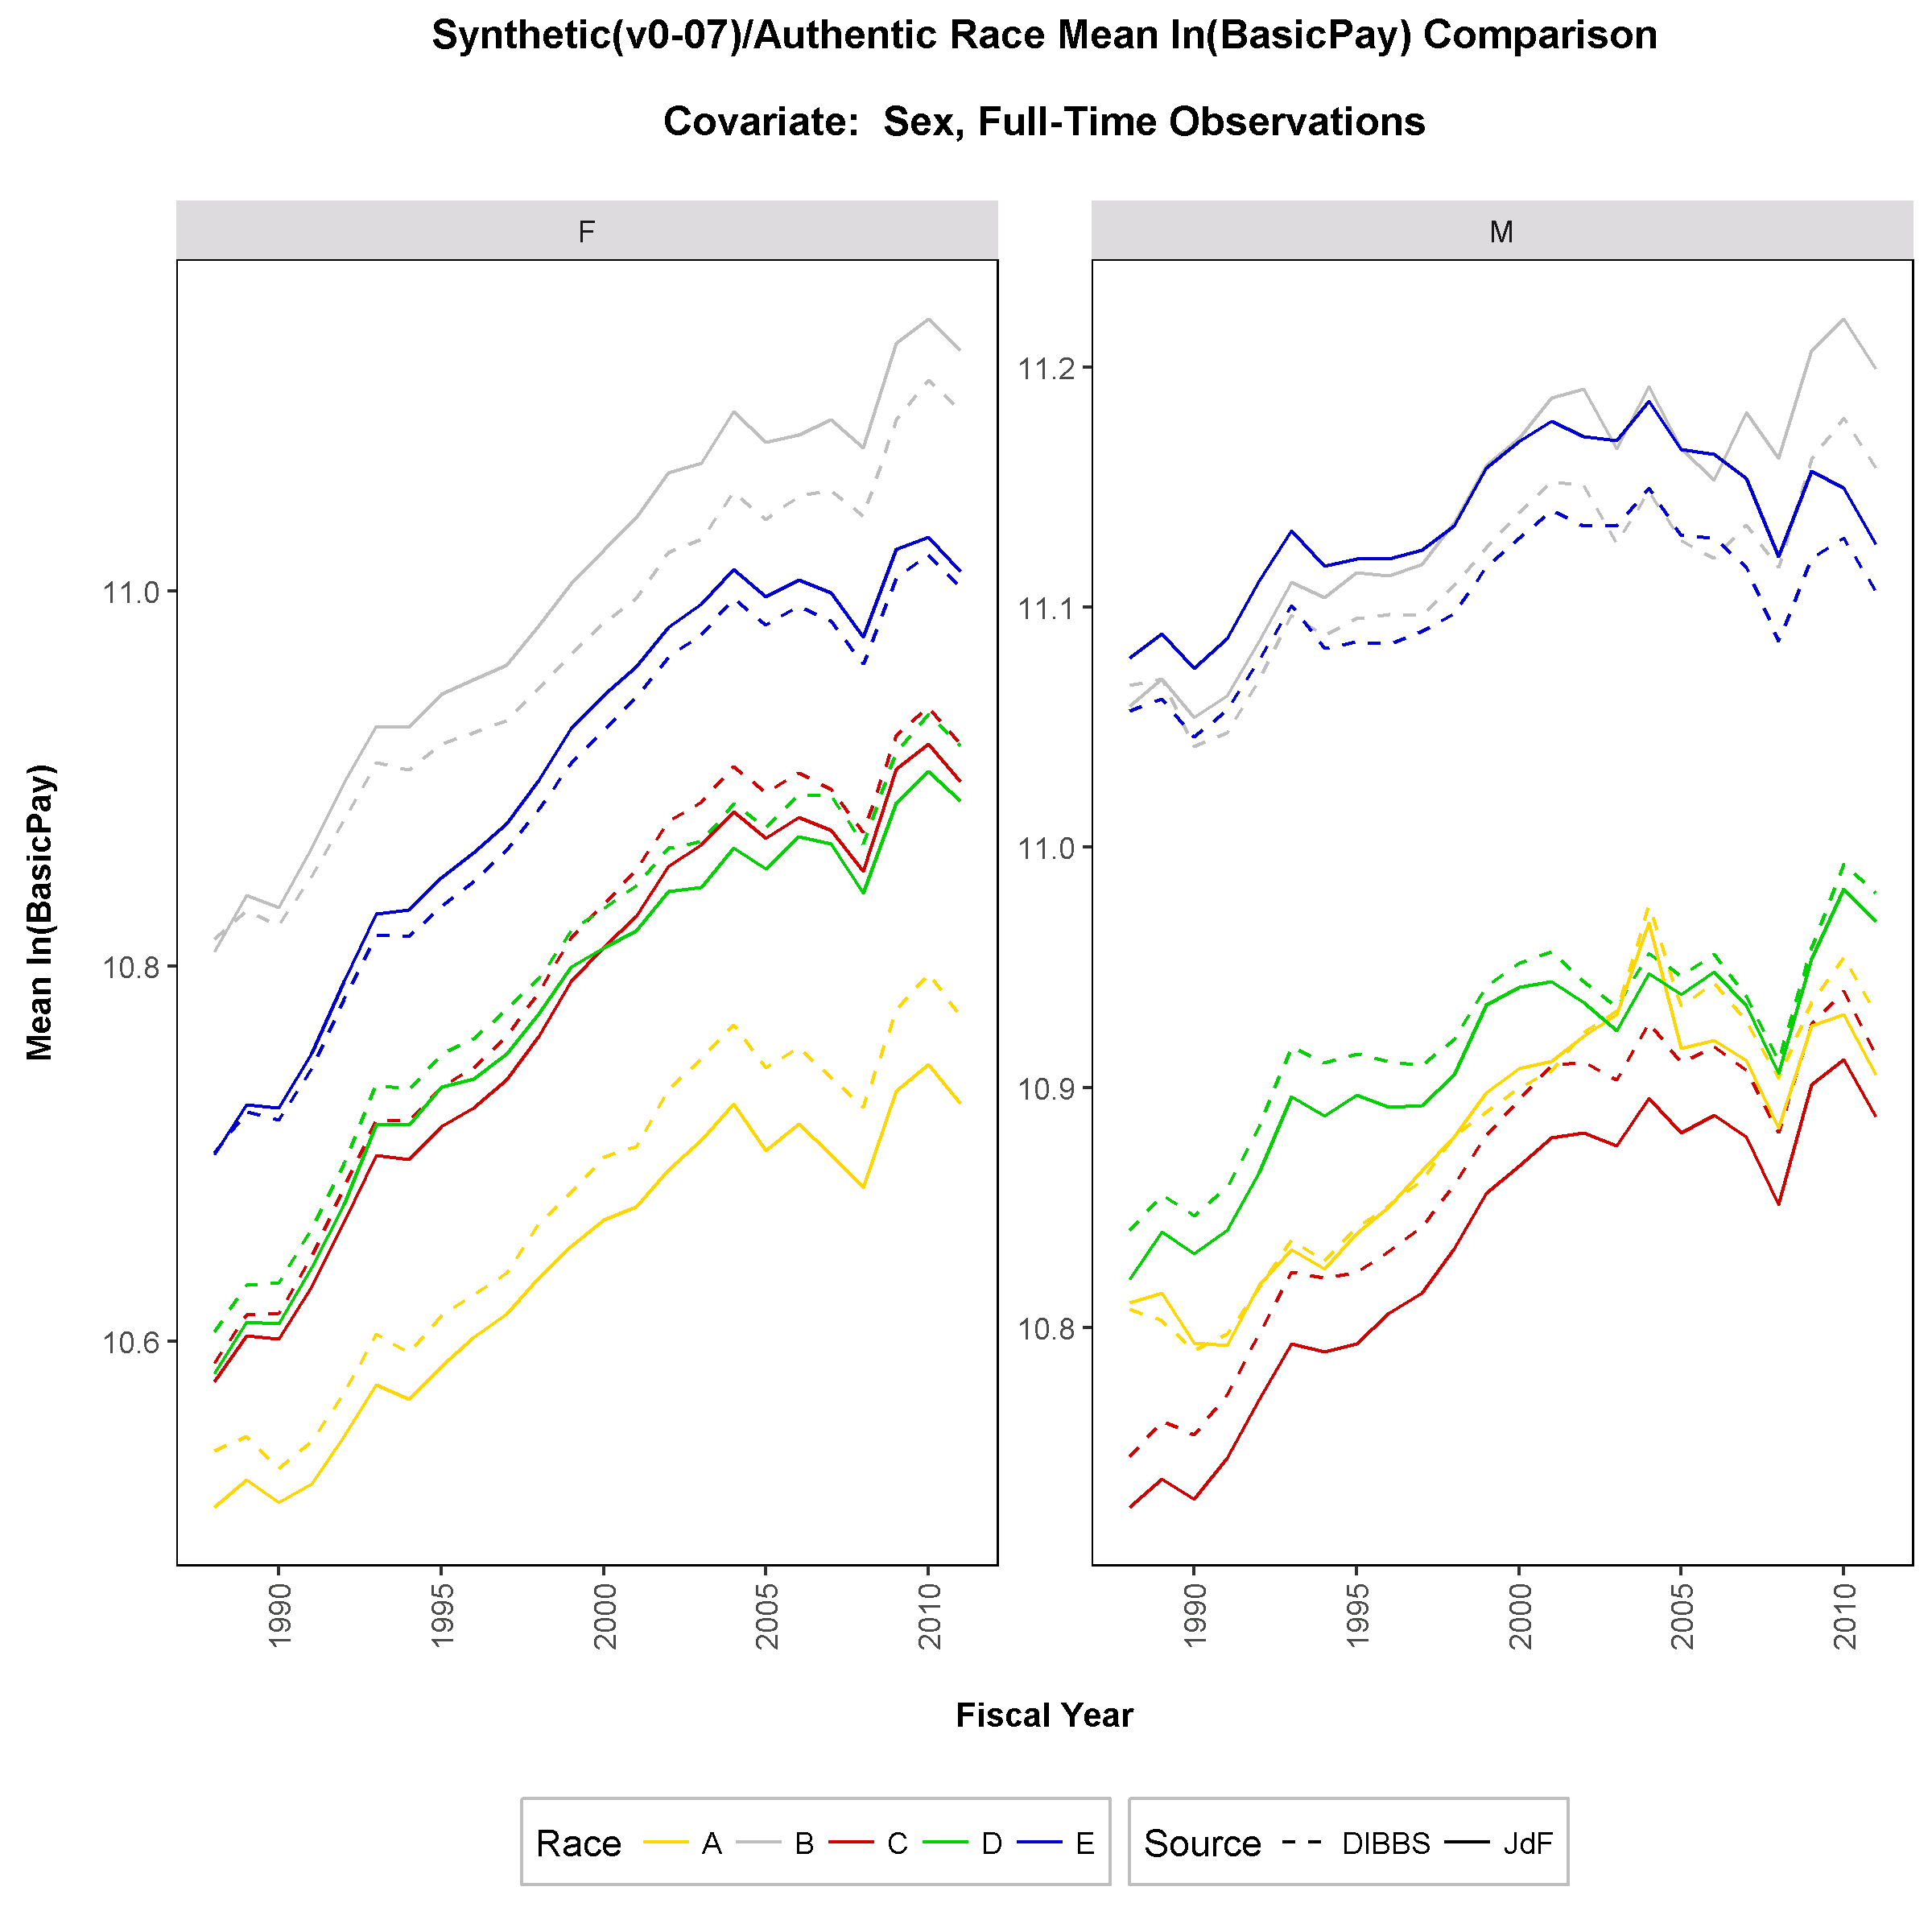
\includegraphics[width=6.5in, trim={0 0 0 0.75in}, clip]{RaceLogPayBySex-FY.png}
    \caption{Mean basic pay by sex, race, and year.  Female on left, male on right.  Race codes:  A = Native American, B = Asian, C = black, D = Hispanic, E = white.  Dashed line for synthetic data, solid line for authentic.}
    \label{figure:RaceLogPayBySex-FY}
\end{figure}

\clearpage

\section{Distribution of Gender}

Disparities in pay, job placement, and promotion with respect to gender are important and common topics in human capital research.  For synthetic data to produce meaningful results, proportion observations by gender must reflect those observed in corresponding authentic data.  This section compares proportions by gender using joint combinations of important organizational and human capital variables.

\subsection{Gender Proportion by Race, Education, and Year}

Accurate proportion observations by gender is critical in reproducing authentic results with models that include gender as an independent variable.  Figure \ref{figure:GenderProportionLogisticModelEducationRaceFYScaleFixedv0-06} plots proportion female employees by race, education, and year.  Fitted lines are logistic regression models.\\

Observation:  This four-way comparison (sex, race, education, and year) confirms good representation in synthetic data of gender proportion among important variable combinations in the authentic data.  Fitted logistic regression models have nearly identical trends through fiscal years.  Note the slight degradation in fit as observation count (n) decreases.\\

\begin{figure}[h]
    \centering
    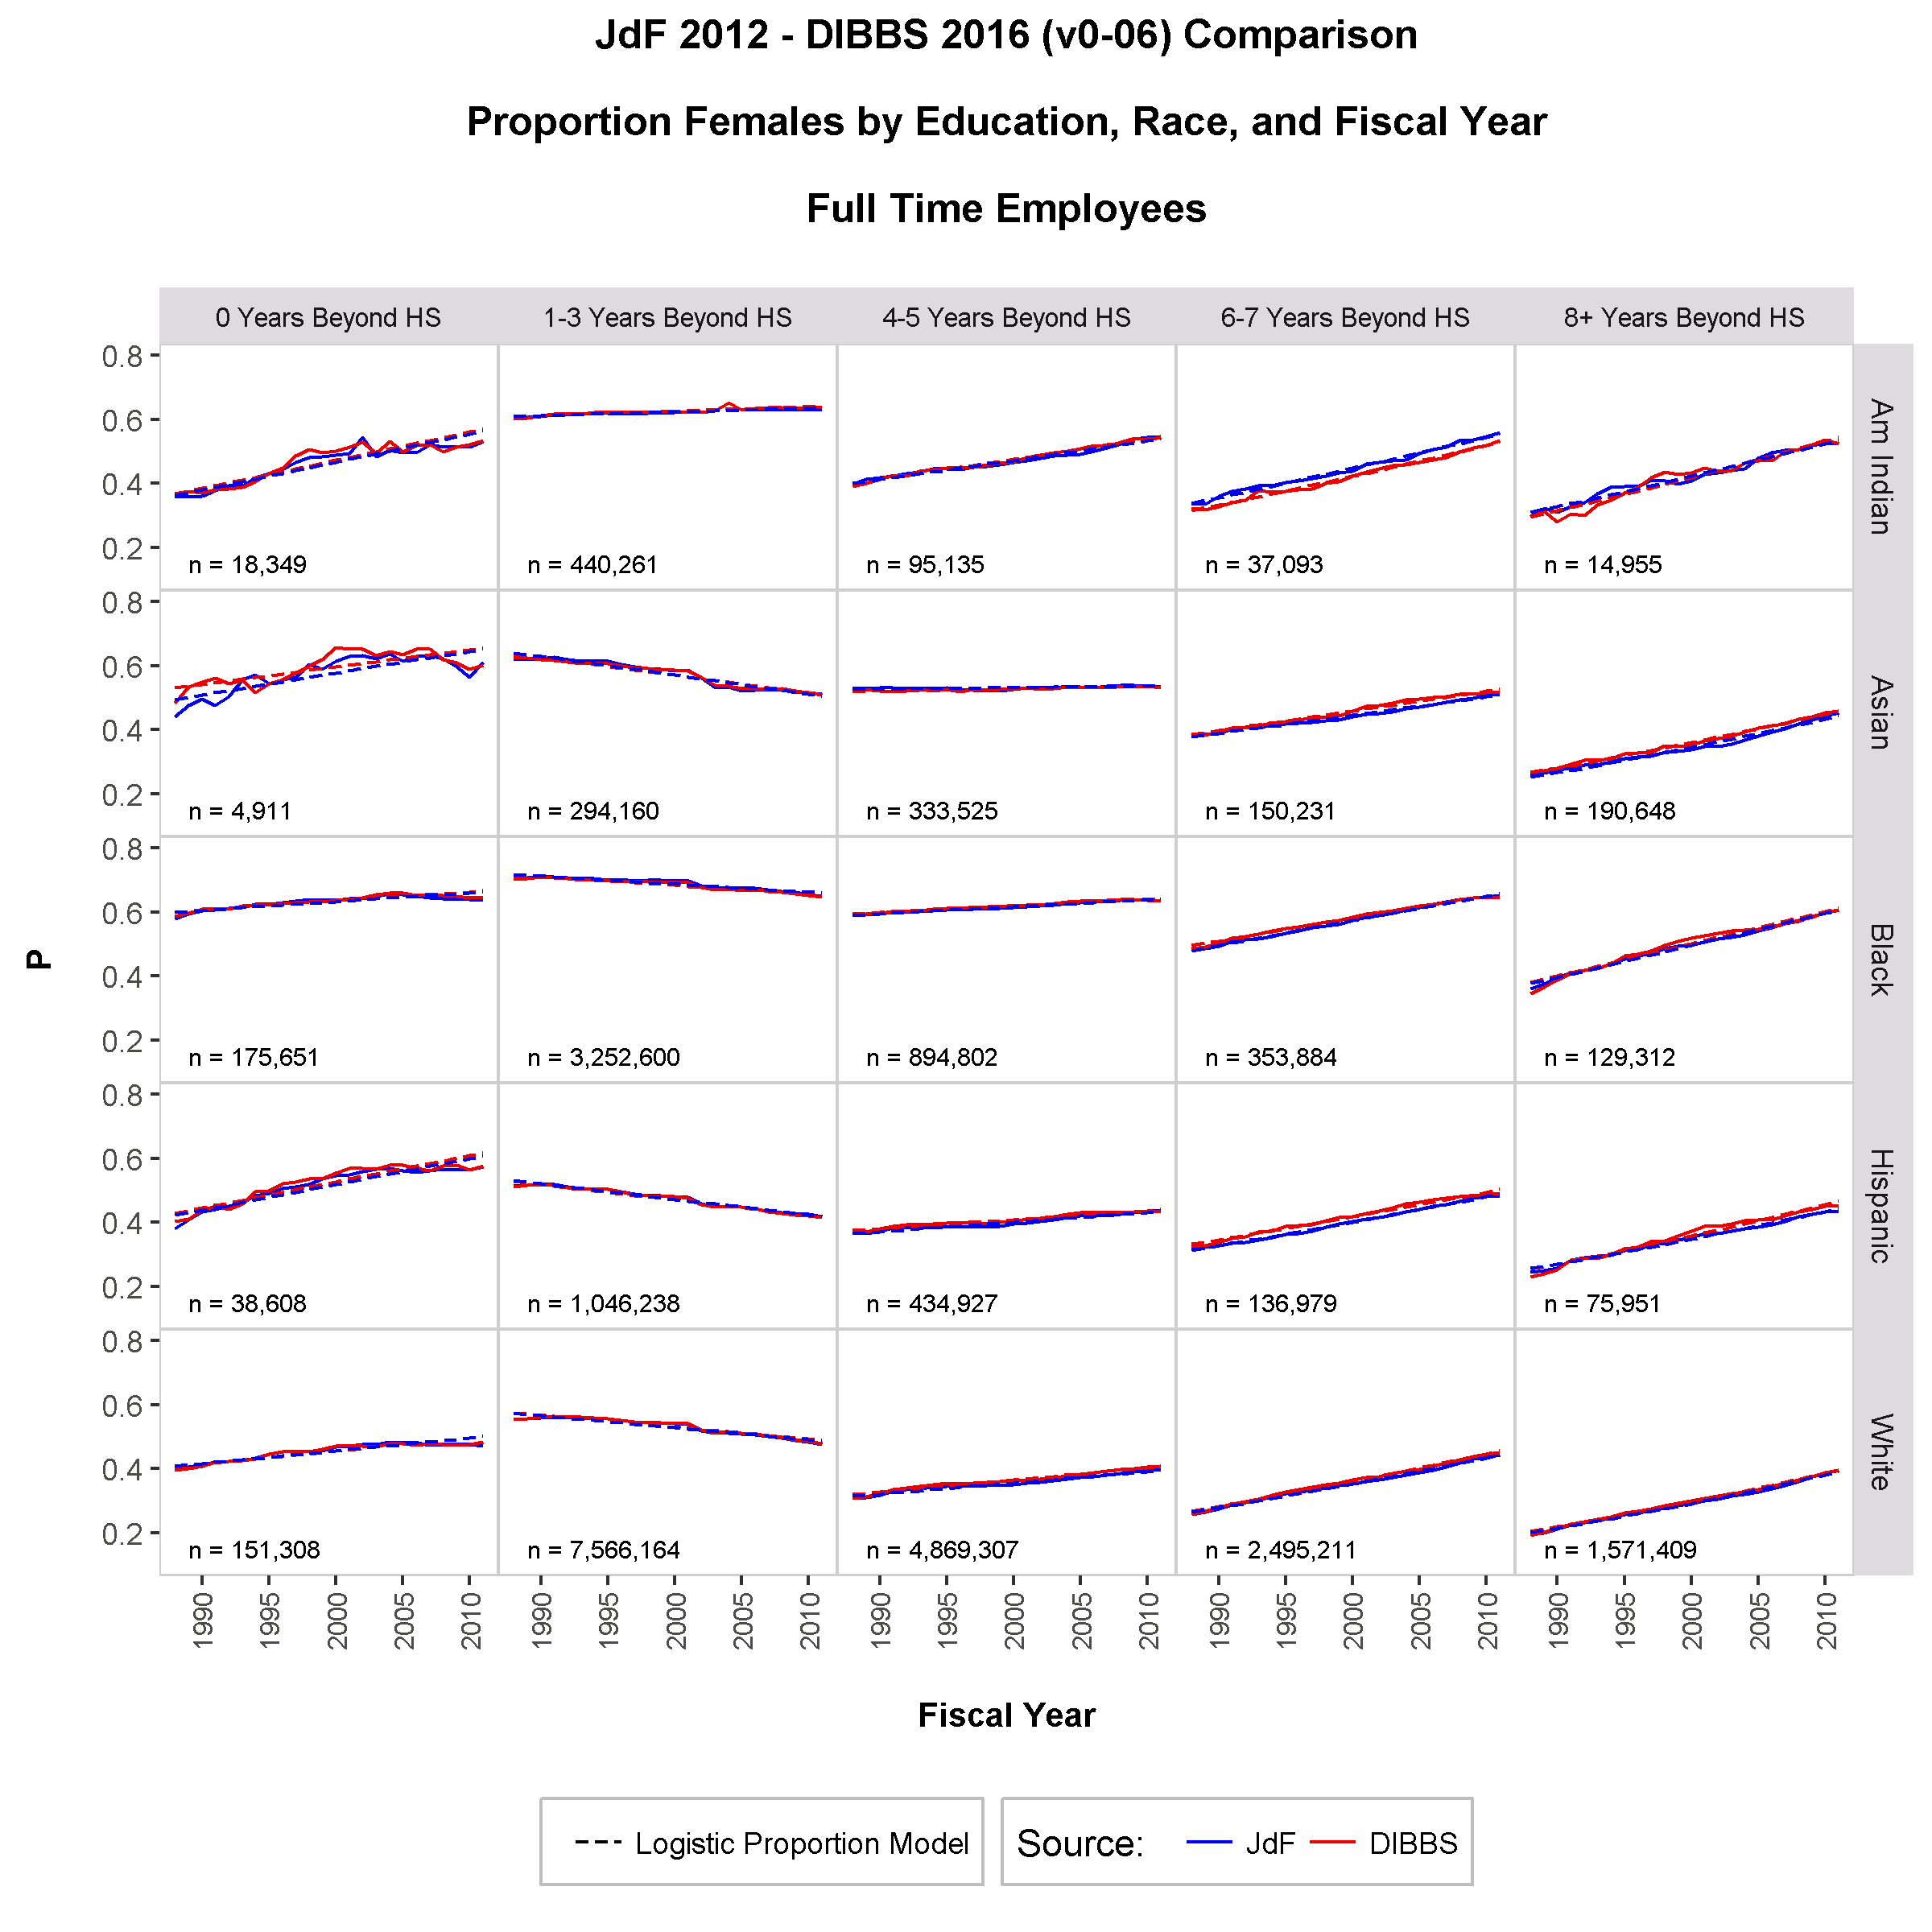
\includegraphics[width=6.25in, trim={0 0 0 1in}, clip]{GenderProportionLogisticModelEducationRaceFYScaleFixedv0-06.png}
    \caption{Proportion female observations by race, education, and year.  Fitted lines are logistic regression estimates.}
    \label{figure:GenderProportionLogisticModelEducationRaceFYScaleFixedv0-06}
\end{figure}

\clearpage

\subsection{Gender Proportion by Race, Age, and Year}

Figures \ref{figure:GenderProportionLogisticModelFYRaceAgeA} through \ref{figure:GenderProportionLogisticModelFYRaceAgeE}, show for each race, proportion female employees by age and year.  Fitted lines are logistic regression models.\\

Observation:  These four-way comparisons (sex, race, age, and year) confirm good representation in synthetic data of gender proportion among important variable combinations in the authentic data.  Through the entire range of fiscal years, logistic regression models derived from synthetic data closely approximate those obtained using authentic data.\\

\vspace{20pt}

\begin{figure}[h]
    \centering
    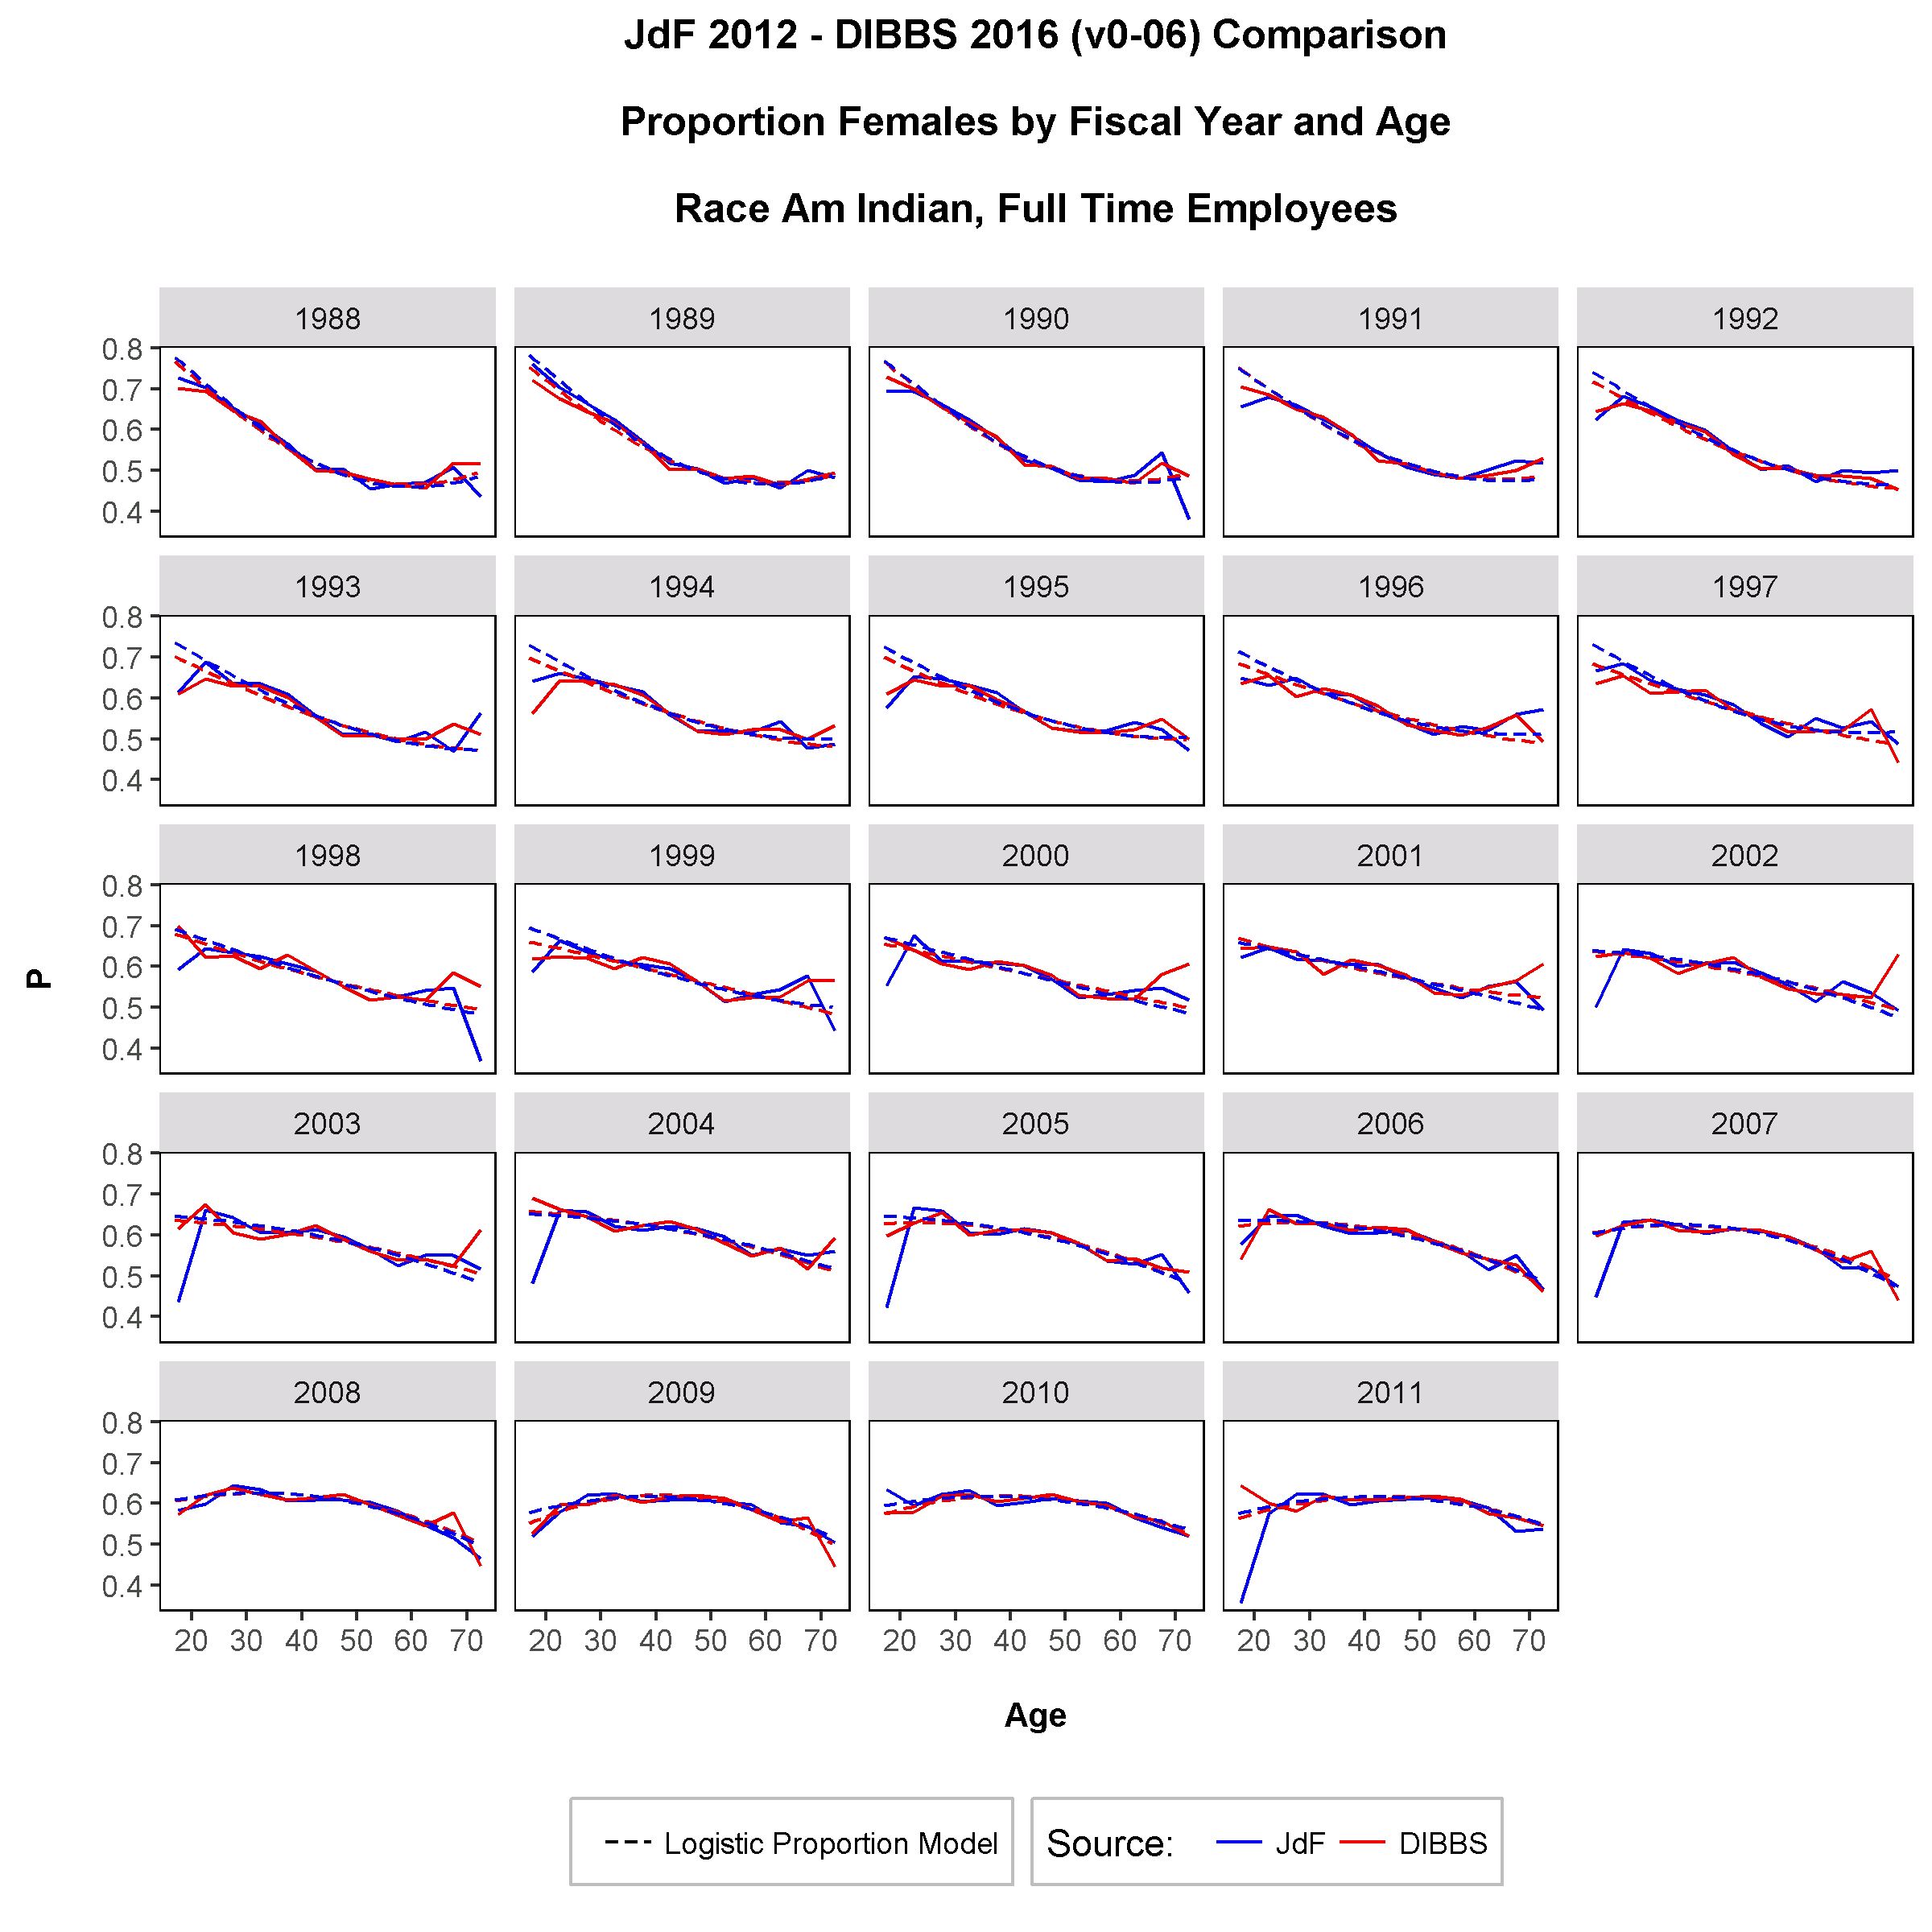
\includegraphics[width=6.5in, trim={0 0 0 1in}, clip]{GenderProportionLogisticModelFYRaceAgeAv0-06.png}
    \caption{Proportion female observations by education and year.  Race Native American.  Fitted lines are logistic regression estimates.}
    \label{figure:GenderProportionLogisticModelFYRaceAgeA}
\end{figure}

\clearpage

\begin{figure}[]
    \centering
    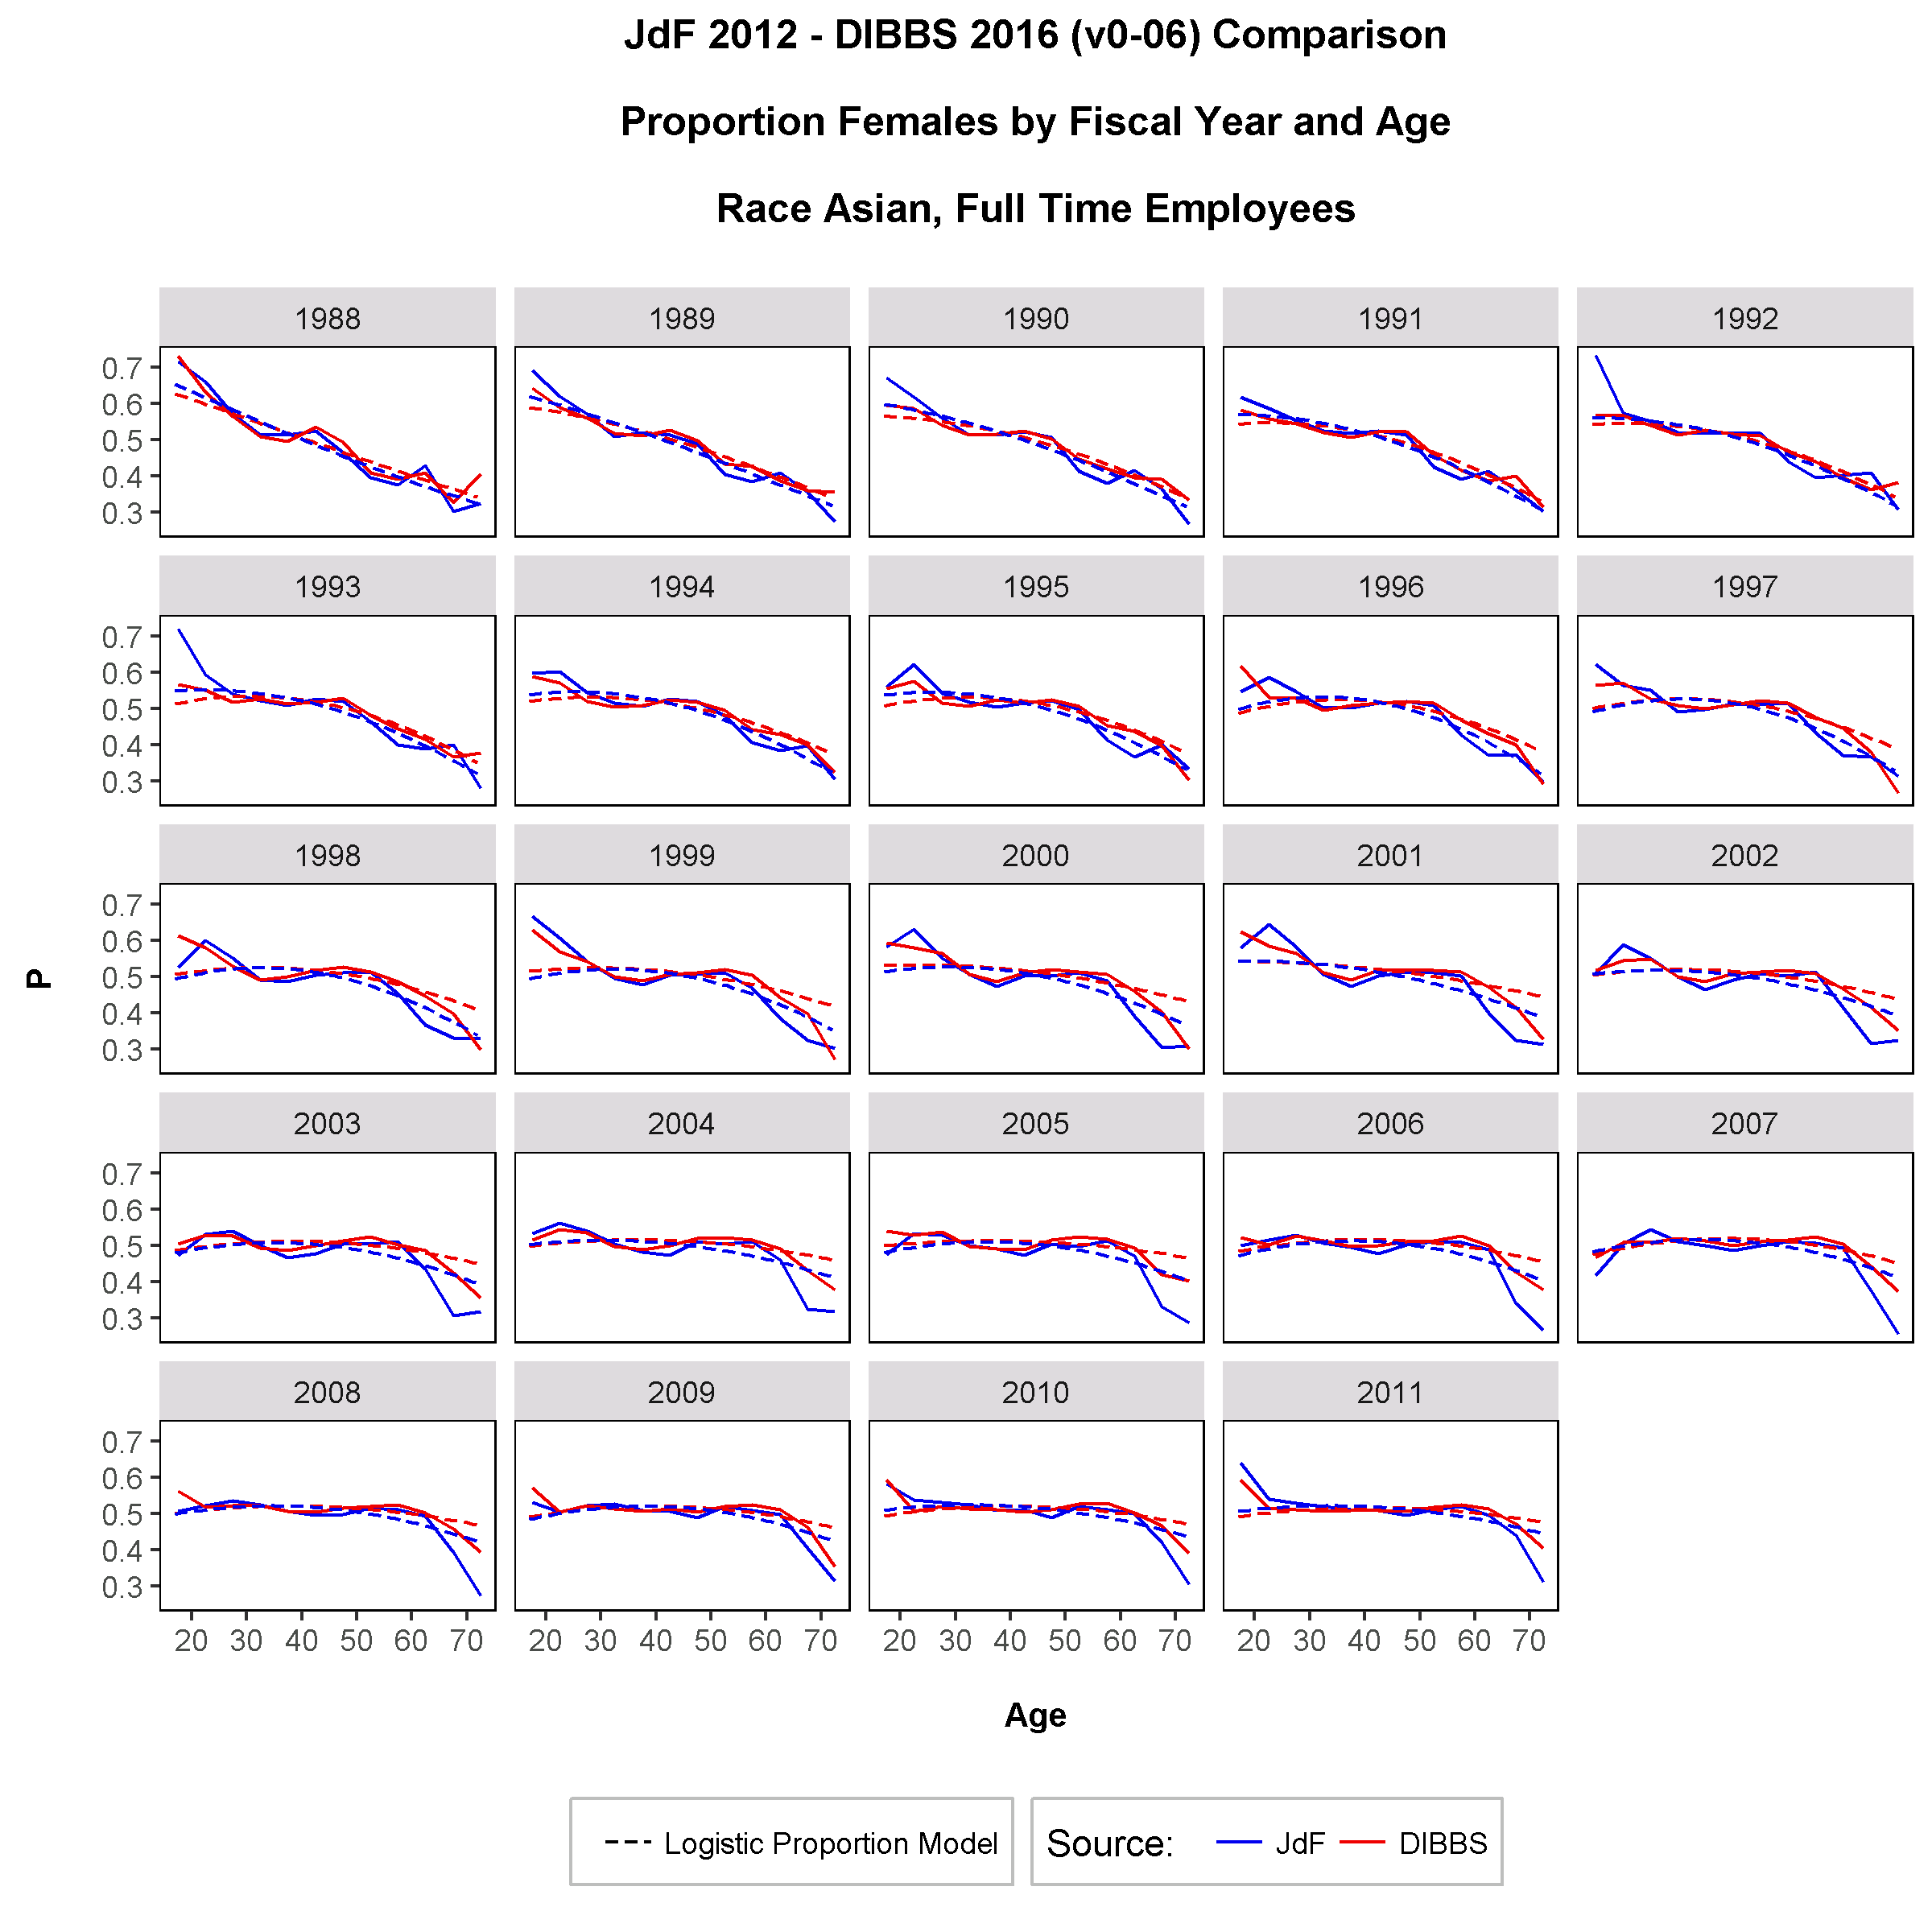
\includegraphics[width=6.5in, trim={0 0 0 1in}, clip]{GenderProportionLogisticModelFYRaceAgeBv0-06.png}
    \caption{Proportion female observations by education and year.  Race Asian.  Fitted lines are logistic regression estimates.}
    \label{figure:GenderProportionLogisticModelFYRaceAgeB}
\end{figure}

\clearpage

\begin{figure}[]
    \centering
    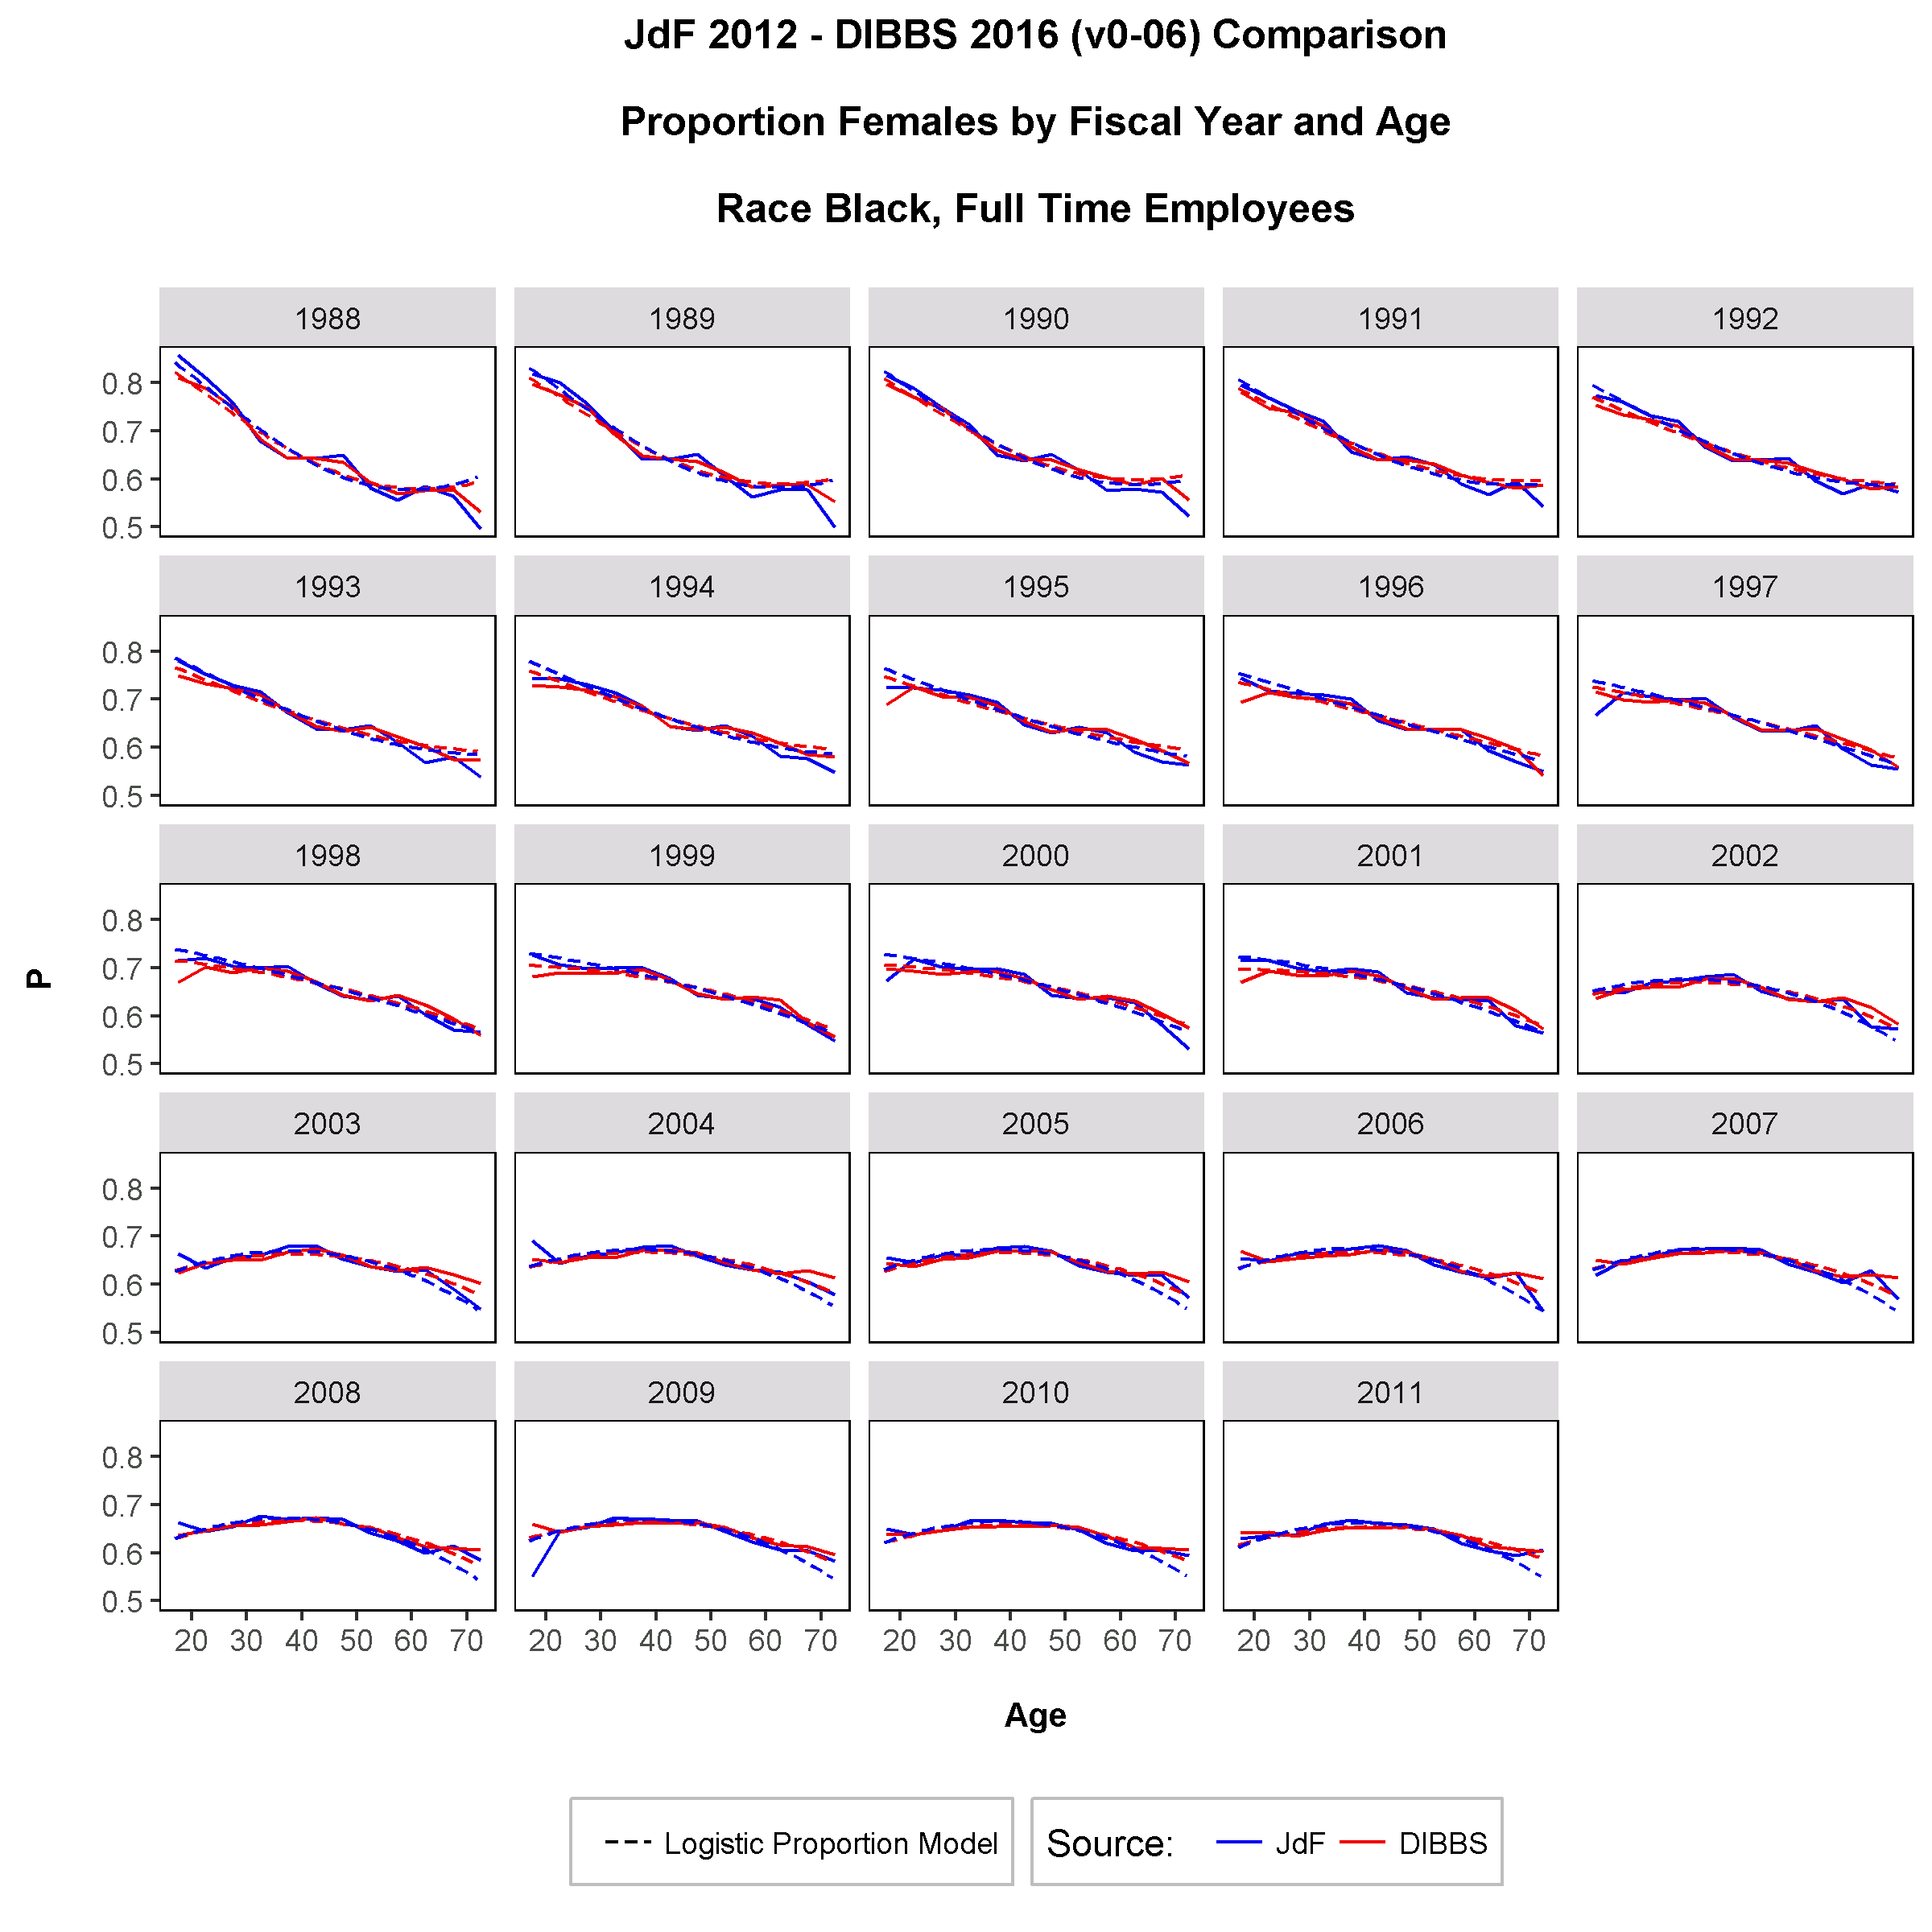
\includegraphics[width=6.5in, trim={0 0 0 1in}, clip]{GenderProportionLogisticModelFYRaceAgeCv0-06.png}
    \caption{Proportion female observations by education and year.  Race black.  Fitted lines are logistic regression estimates.}
    \label{figure:GenderProportionLogisticModelFYRaceAgeC}
\end{figure}

\clearpage

\begin{figure}[]
    \centering
    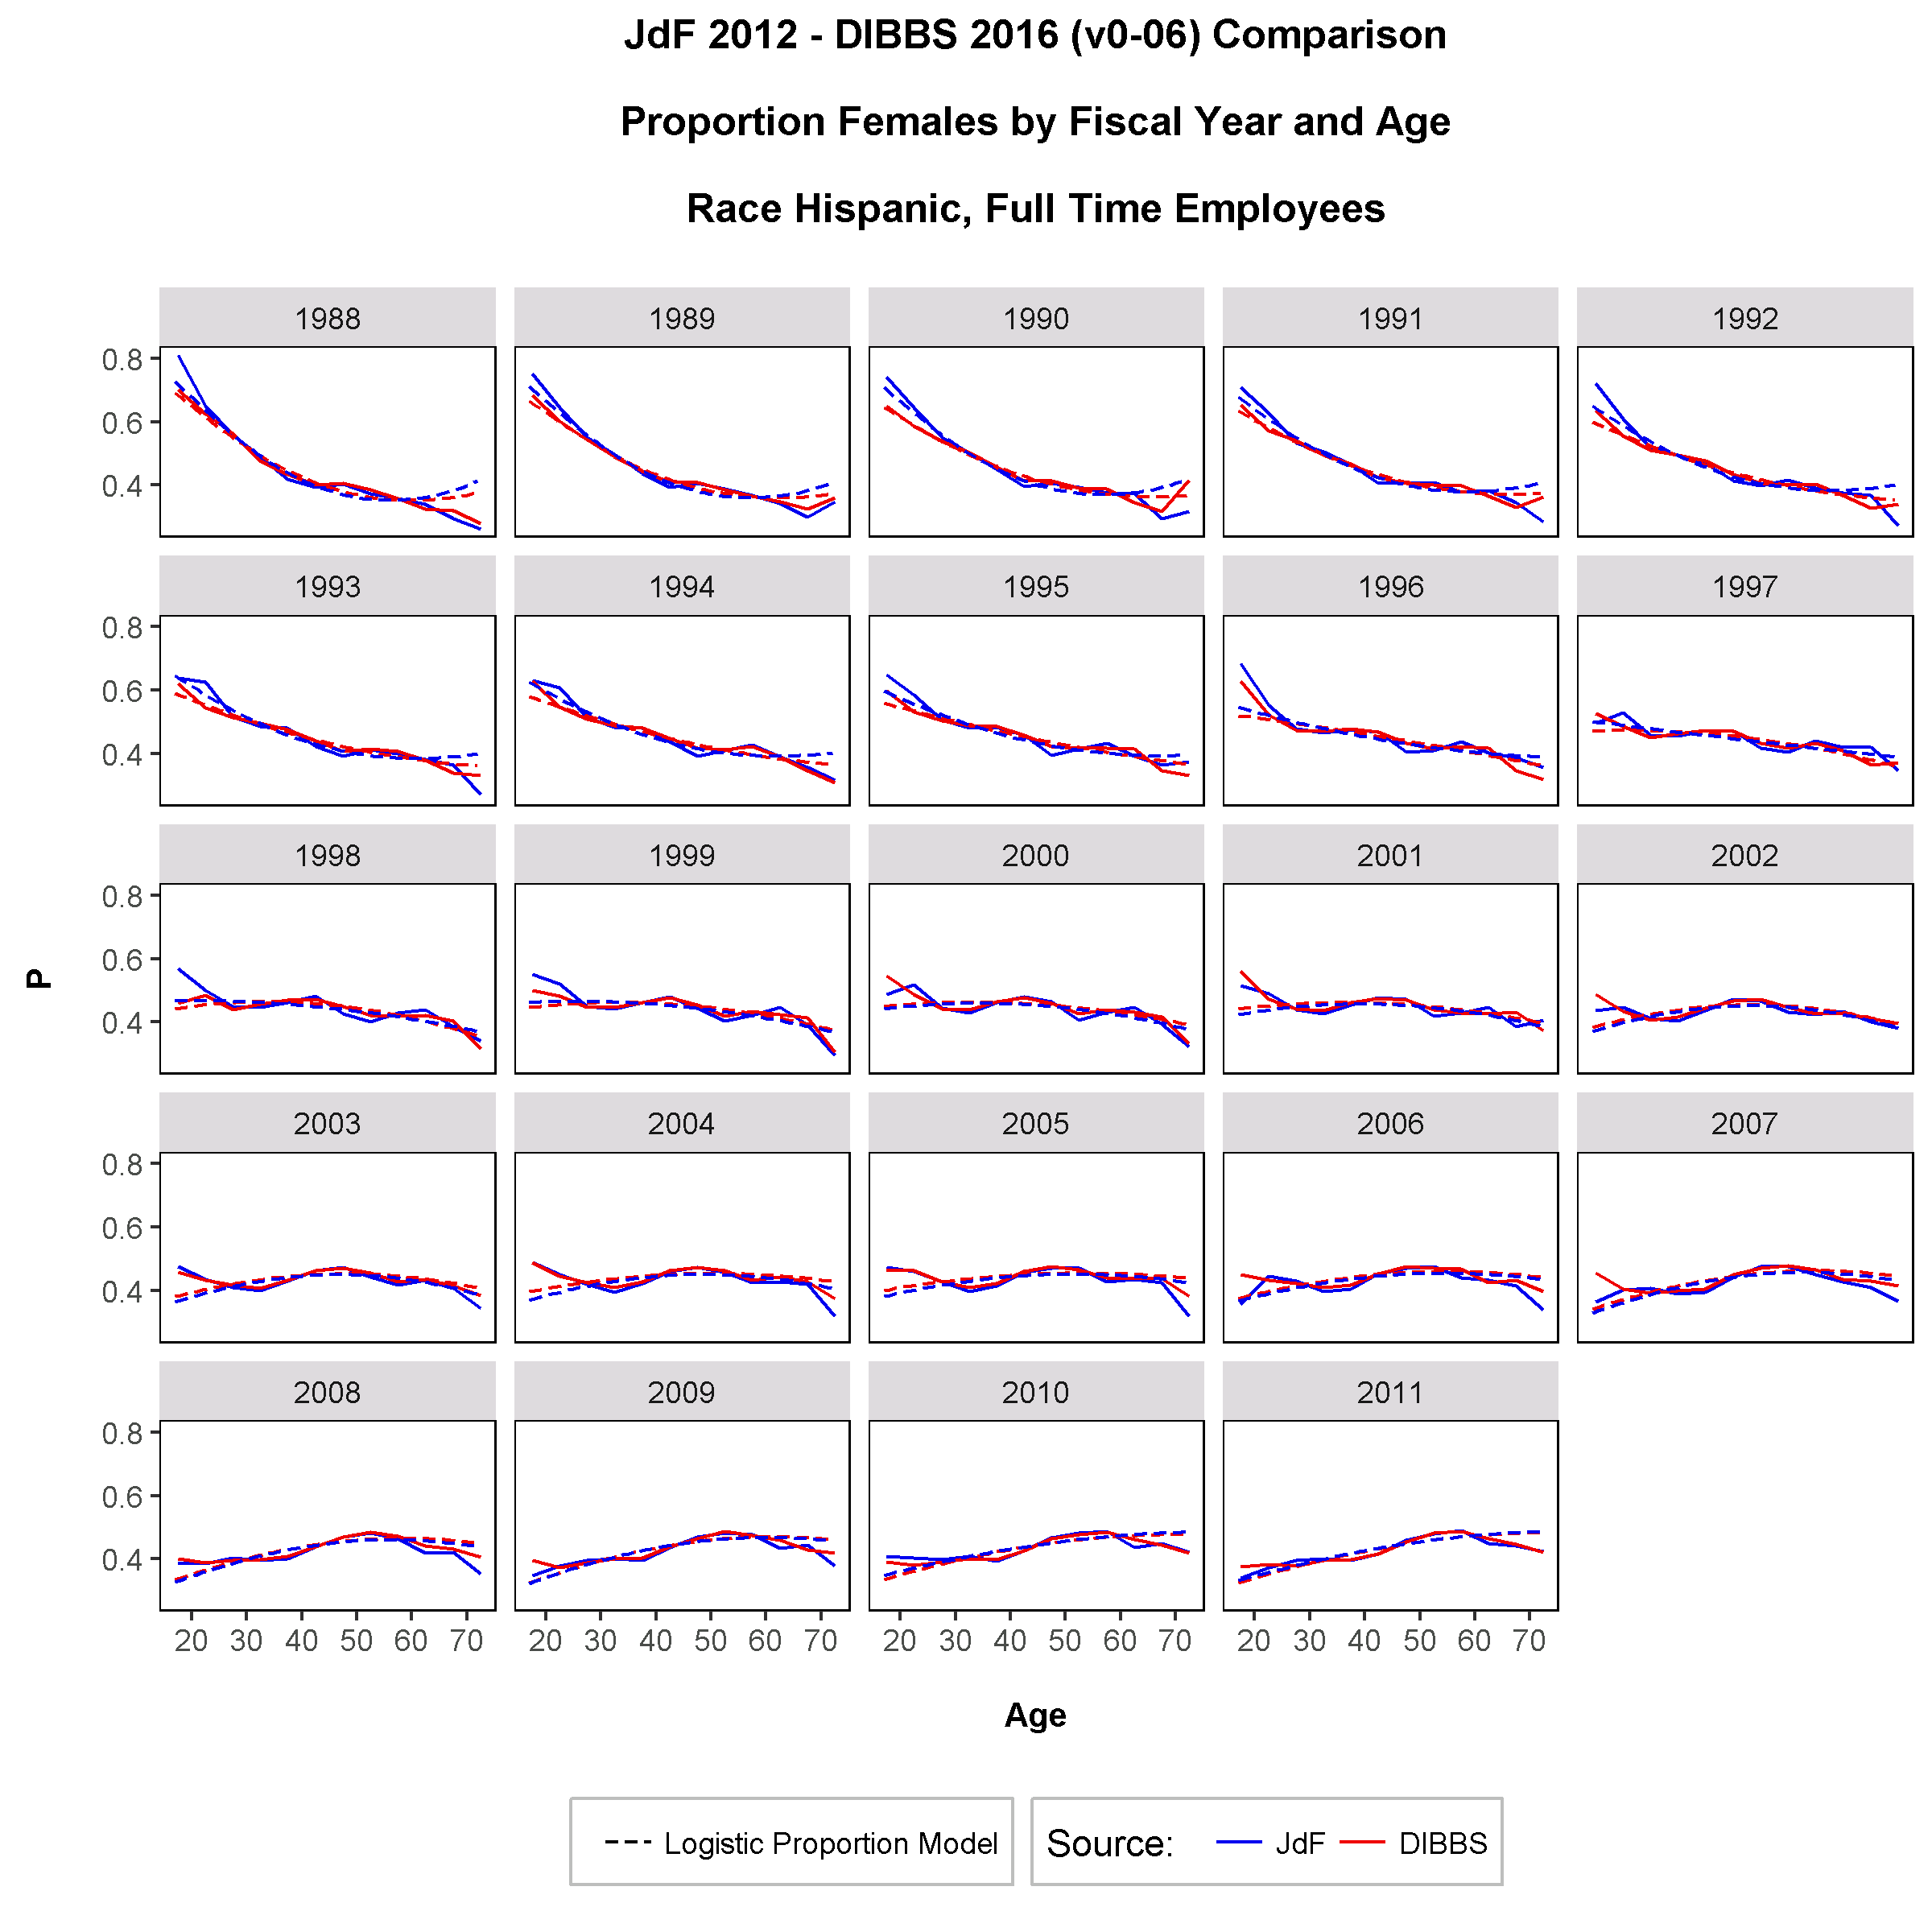
\includegraphics[width=6.5in, trim={0 0 0 1in}, clip]{GenderProportionLogisticModelFYRaceAgeDv0-06.png}
    \caption{Proportion female observations by education and year.  Race Hispanic.  Fitted lines are logistic regression estimates.}
    \label{figure:GenderProportionLogisticModelFYRaceAgeD}
\end{figure}

\clearpage

\begin{figure}[]
\centering
\includegraphics[width=6.5in, trim={0 0 0 1in}, clip]{GenderProportionLogisticModelFYRaceAgeEv0-06.png}
\caption{Proportion female observations by education and year.  Race white.  Fitted lines are logistic regression estimates.}
\label{figure:GenderProportionLogisticModelFYRaceAgeE}
\end{figure}

\clearpage

\subsection{Gender Proportion by Occupation}

In the data supplied by OPM, 205 occupations (more than 25\%) have proportion female observations below 0.05.  12 have proportion female observations greater than 0.95.  Of these occupations, 148 have fewer than 1,000 total observations and 30 haver fewer than 10 observations.  This presents challenges for accurate representation of authentic proportions in synthetic observations, while reducing the risk of individual employee identification.  Figures \ref{figure:JdFDIBBSOccupationProportionBar1} and \ref{figure:JdFDIBBSOccupationProportionBar2} compare proportion female for the first 120 occupation codes.  Figures \ref{figure:JdFDIBBSOccupationProportionBar3} and \ref{figure:JdFDIBBSOccupationProportionBar4} compare proportions for the first 120 trade occupations, which begin at code 2500.  ``n-DIBBS" indicates synthetic observation count, ``n-JdF" indicates corresponding authentic observation count.\\

Observation:  Agreement for large count occupations is indicated by proximity of points.  Departure increases with decrease in observation count.  Trade occupations, having generally low observation count and low proportion female in the authentic data, exhibit greater discrepancies than those observed in non-trade occupations.\\

\begin{figure}[h]
    \centering
    \begin{subfigure}{1\textwidth}
        \centering
        \includegraphics[width=6in, trim={0 1in 0 1in}, clip]{JdFDIBBSOccupationProportionBar1.png}
        \caption{Occupations 0006 through 0135}
        \vspace{10pt}
    \end{subfigure}
    \begin{subfigure}{1\textwidth}
        \centering
        \includegraphics[width=6in, trim={0 1in 0 1in}, clip]{JdFDIBBSOccupationProportionBar41.png}
        \caption{Occupations 0136 through 0302}
        \vspace{10pt}
    \end{subfigure}
    \caption{Proportion female observations by occupation.  All agencies combined.  One synthetic and one authentic point per occupation.  Occupation on x-axis.}
    \label{figure:JdFDIBBSOccupationProportionBar1}
\end{figure}

\clearpage

\begin{figure}[h]
    \centering
    \begin{subfigure}{1\textwidth}
        \centering
        \includegraphics[width=6in, trim={0 1in 0 1in}, clip]{JdFDIBBSOccupationProportionBar81.png}
        \caption{Occupations 0303 through 0399}
        \vspace{10pt}
    \end{subfigure}
    \begin{subfigure}{1\textwidth}
        \centering
        \includegraphics[width=6in, trim={0 1in 0 1in}, clip]{JdFDIBBSOccupationProportionBar121.png}
        \caption{Occupations 0401 through 0512}
        \vspace{10pt}
    \end{subfigure}
    \caption{Proportion female observations by occupation.  All agencies combined.  One synthetic and one authentic point per occupation.  Occupation on x-axis.}
    \label{figure:JdFDIBBSOccupationProportionBar2}
\end{figure}

\clearpage

\begin{figure}[h]
    \centering
    \begin{subfigure}{1\textwidth}
        \centering
        \includegraphics[width=6in, trim={0 1in 0 1in}, clip]{JdFDIBBSOccupationProportionBar481.png}
        \caption{Occupations 2502 through 3511 (trades)}
        \vspace{10pt}
    \end{subfigure}
    \begin{subfigure}{1\textwidth}
        \centering
        \includegraphics[width=6in, trim={0 1in 0 1in}, clip]{JdFDIBBSOccupationProportionBar521.png}
        \caption{Occupations 3513 through 3911 (trades)}
        \vspace{10pt}
    \end{subfigure}
    \caption{Proportion female observations by occupation.  All agencies combined.  One synthetic and one authentic point per occupation.  Occupation on x-axis.}
    \label{figure:JdFDIBBSOccupationProportionBar3}
\end{figure}

\clearpage

\begin{figure}[h]
    \centering
    \begin{subfigure}{1\textwidth}
        \centering
        \includegraphics[width=6in, trim={0 1in 0 1in}, clip]{JdFDIBBSOccupationProportionBar561.png}
        \caption{Occupations 3940 through 4605 (trades)}
        \vspace{10pt}
    \end{subfigure}
    \begin{subfigure}{1\textwidth}
        \centering
        \includegraphics[width=6in, trim={0 1in 0 1in}, clip]{JdFDIBBSOccupationProportionBar601.png}
        \caption{Occupations 4607 through 5306 (trades)}
        \vspace{10pt}
    \end{subfigure}
    \caption{Proportion female observations by occupation.  All agencies combined.  One synthetic and one authentic point per occupation.  Occupation on x-axis.}
    \label{figure:JdFDIBBSOccupationProportionBar4}
\end{figure}

\clearpage

\subsection{Occupation Gender Proportion Kernel Density}

Figure \ref{figure:JdFDIBBSProportionFemaleDistributionByOccupation-v0-06} superimposes synthetic and authentic kernel density plots of proportion female employees by occupation.\\

Observations:  There is some discrepancy in density for synthetic proportions near 0 and above 0.75, which is compensated for near more central proportions.  Since very low or very high proportion observations within important identifiers (sex in this case) can promote individual identification, discrepancies in extremes may be expected.\\

\vspace{20pt}

\begin{figure}[h]
    \centering
    \includegraphics[width=6in, trim={0 0 0 1in}, clip]{JdFDIBBSProportionFemaleDistributionByOccupation-v0-06.png}
    \caption{Occupation proportion female kernel density.  Synthetic and authentic distributions superimposed.  Trade occupations slightly over-represented near zero and above 0.75 in authentic data.  Slight discrepancy in synthetic proportions at extremes.  Compensated for near central proportions.}
    \label{figure:JdFDIBBSProportionFemaleDistributionByOccupation-v0-06}
\end{figure}

\clearpage

\subsection{Gender Proportion Logistic Regression Classifier for Trade Occupations}

A gender classifier for occupations with code greater 2500 (trades) using the logistic regression model
\begin{center} $\mest{p}=f(\mest{\beta}_{race}race+\mest{\beta}_{age}age+\mest{\beta}_{age^2}age^2+
    \mest{\beta}_{ed}ed+\mest{\beta}_{ed^2}ed^2+\mest{\beta}_{occ}occ)$,\\
\end{center}
where $f()$ estimates proportion female observations by race, age, education, and occupation, was used to classify sex, such that all observations associated with combinations of independent variables with $\mest{p}\ge$0.5 are classified as female.  Figure \ref{figure:GenderProportionROCAgeAgeSqEdEdSqRaceOccGE2500ByFYv0-06} plots, for fiscal years 1988-2011 (all years supplied by OPM) and $\mest{p}$ values from 0 to 1.0, the proportion of accurate female observation classification (y-axis) against the proportion accurate male classification (x-axis).\\

Observation:  Although the classifiers, exhibiting somewhat flat ROC curves (near the $\mest{p}$=0.5 reference line of slope 1.0) appear to be of limited utility, those derived from synthetic data are nearly identical their counterparts derived from authentic data, including an apparent reduction in utility (nearer to the reference line) as fiscal years advance.  Incidentally, the reduced utility with year may reflect structural changes in proportion female for trade occupations during this period.\\

\begin{figure}[h]
    \centering
    \includegraphics[width=5in, trim={0 0.75in 0 1in}, clip]{GenderProportionROCAgeAgeSqEdEdSqRaceOccGE2500ByFYv0-06.png}
    \caption{Proportion female race, age, education, occupation classifier ROC curves.  One curve per data set per by fiscal.  Agreement in classifier accuracy indicated by overlapping curves. Pattern of decreased accuracy as years progress captured in both data sets. }
    \label{figure:GenderProportionROCAgeAgeSqEdEdSqRaceOccGE2500ByFYv0-06}
\end{figure}

\clearpage

\section{Gender Pay Disparity Fixed Effects Models}

\subsection{Fixed Effects Ordinary Least Squares Regression Model}

In their study of pay disparity in the federal government, Alexander Bolton and John de Figueiredo report an effect of gender on difference in basic pay using fixed effects regression models that control for important human capital factors \citep{BoltondeFigGenderPayGap2017}.  An example model is

\vspace{-10pt}
\begin{equation} y=\beta_0+\beta_ffemale+\beta_rrace+\beta_{ag}age+\beta_{ag^2}age^2+\beta_{ed}education+\beta_{bur}bureau+\beta_{occ}occupation+\beta_{yr}year
\label{model:GenderPayOLS}
\end{equation}

where $y$ is the expected value of log(basic pay), given specific levels of race, age, years of education, bureau (proxy for agency), occupation, and year.  Using \textit{male} as the sex reference level, $\mest{\beta}_f$, estimated from model (\ref{model:GenderPayOLS}), measures the difference in pay between females and males after correcting for the remaining variables.  Table \ref{table:GenderPayOLS} lists parameter estimates for model (\ref{model:GenderPayOLS}) fit to full-time, pay plan GS synthetic and authentic observations.  Common reference levels were used for both sets (sex male, race white, highest frequency bureau and occupation, and fiscal year 1988).  Corresponding standard errors appear in parentheses beneath each estimate.\footnote{Although Bolton and de Figueiredo compute robust standard errors clustered about employee, for simplicity we ignore potential heteroskedasticity of residuals and present here homoskedastic residual based standard errors estimated using the diagonal of the inverse of the covariance matrix.}  Figure \ref{figure:DIBBSEstimateVsJdFEstimateNoInterceptGSPayPlanFixedRefLevel} plots 
synthetic data estimates for model (\ref{model:GenderPayOLS}) against corresponding authentic data estimates, one point for each estimate.  The ``X" group includes estimates for sex, race, education, and age.  Figures \ref{figure:DIBBSEstimateVsJdFEstimateNoInterceptGSPayPlanFixedRefLevel-X}, \ref{figure:DIBBSEstimateVsJdFEstimateNoInterceptGSPayPlanFixedRefLevel-Bureau}, and \ref{figure:DIBBSEstimateVsJdFEstimateNoInterceptGSPayPlanFixedRefLevel-Occupation} plot parameter estimates obtained by fitting model (\ref{model:GenderPayOLS}) to annual subsets of synthetic and authentic data.  These are used to identify potential patterns of change in parameter estimate association throughout the study period.\\

Observations (table):  Although some discrepancies exist between estimates from the two data sets, the close proximity of $\mest{\beta}_f$ estimates confirms the utility of synthetic data results for gender pay disparity research.\footnote{Some deviations in parameter estimates may appear large with respect to corresponding standard errors.  However, due to relatively large observation counts, n, standard errors are small, implying that the data sets are more like populations than samples, which magnifies deviations and calls into question customary notions of parameter estimate distribution.}  In their analysis, Bolton and de Figueiredo conclude that the reported pay disparity of approximately -0.03 is significant.  Using the synthetic data, a researcher would measure very similar disparity and, presumably, reach a similar conclusion of significance.\\

Observations (figure \ref{figure:DIBBSEstimateVsJdFEstimateNoInterceptGSPayPlanFixedRefLevel}):  Points generally lie near the reference line of slope 1.0, indicating overall agreement of synthetic and authentic parameter estimates.  Light dots indicate low frequency bureaus and occupations and represent most of the large deviations from reference lines.\\

Observations (annual figures):  Points generally lie near reference lines in all years for the three groups.  Low frequency bureaus and occupations (light dots) account for deviations from reference.  There does not appear to be any pattern of change in association of estimates between data sets throughout the period.

\begin{table}[h]
    \centering
    \caption{Parameter estimates from gender pay disparity fixed effects model}
    \label{table:GenderPayOLS}
    \begin{tabular}{lrr}
        \hline\\[-10pt]
        Parameter Estimate & OPM & DIBBS \\ 
        \hline\\[-6pt]
        \hspace{10pt} $\mest{\beta}_0$ & 9.3973 & 9.6167 \\ 
        & (7.19e-04) & (7.23e-04) \\ 
        \hspace{10pt} $\mest{\beta}_f$ & -0.0319 & -0.0296 \\ 
        & (1.10e-04) & (1.17e-04) \\ 
        \hspace{10pt} $\mest{\beta}_{age}$ & 0.0352 & 0.0269 \\ 
        & (2.93e-05) & (2.85e-05) \\ 
        \hspace{10pt} $\mest{\beta}_{age^2}$ & -0.0003 & -0.0002 \\ 
        & (3.29e-07) & (3.19e-07) \\ 
        \hspace{10pt} $\mest{\beta}_{ed}$ & 0.0186 & 0.0122 \\ 
        & (2.69e-05) & (2.78e-05) \\ 
        \hspace{10pt} $\mest{\beta}_{raceAmInd}$ & -0.0370 & -0.0161 \\ 
        & (4.03e-04) & (4.12e-04) \\ 
        \hspace{10pt} $\mest{\beta}_{raceAsian}$ & -0.0320 & -0.0253 \\ 
        & (2.53e-04) & (2.70e-04) \\ 
        \hspace{10pt} $\mest{\beta}_{raceBlack}$ & -0.0095 & -0.0057 \\ 
        & (1.25e-04) & (1.34e-04) \\ 
        \hspace{10pt} $\mest{\beta}_{raceHisp}$ & -0.0202 & -0.0137 \\ 
        & (1.85e-04) & (1.99e-04) \\ 
        \hspace{10pt} $\mest{\beta}_{bureau}$ & & 332 fixed effect levels \\ 
        \hspace{10pt} $\mest{\beta}_{occupation}$ & & 466 fixed effect levels \\ 
        \hspace{10pt} $\mest{\beta}_{year}$ & & 23 fixed effect levels \\
        \hspace{10pt} n & 18,165,075 & 18,714,815 \\[4pt]
        \hline
    \end{tabular}
\end{table}

\clearpage

\begin{figure}[]
    \centering
    \includegraphics[width=6in, trim={0 0 0 1.5in}, clip]{DIBBSEstimateVsJdFEstimateNoInterceptGSPayPlanFixedRefLevel.png}
    \caption{Pay disparity fixed effects regression model parameter estimates.  X group includes estimates for sex, race, education, and age.  Points lie near reference line of slope 1.0, indicating general agreement of synthetic and authentic parameter estimates.  Light dots represent low frequency bureaus and occupations.  They are associated with large deviations from reference line.}
    \label{figure:DIBBSEstimateVsJdFEstimateNoInterceptGSPayPlanFixedRefLevel}
\end{figure}

\clearpage

\begin{figure}[]
    \centering
    \includegraphics[width=6in, trim={0 0 0 1in}, clip]{DIBBSEstimateVsJdFEstimateNoInterceptGSPayPlanFixedRefLevel-X.png}
    \caption{Sex (female), race, age, $\text{age}^2$, and years of education parameter estimates from annual pay disparity fixed effects regression model.  Points near reference line, indicating similarity.  No pattern of change throughout study period.}
    \label{figure:DIBBSEstimateVsJdFEstimateNoInterceptGSPayPlanFixedRefLevel-X}
\end{figure}

\clearpage

\begin{figure}[]
    \centering
    \includegraphics[width=6in, trim={0 0 0 1in}, clip]{DIBBSEstimateVsJdFEstimateNoInterceptGSPayPlanFixedRefLevel-Bureau.png}
    \caption{Bureau (agency) parameter estimates from annual pay disparity fixed effects regression model.  Points near reference line, indicating similarity.  Light points away from reference represent low frequency bureaus.  No pattern of change throughout study period.}
    \label{figure:DIBBSEstimateVsJdFEstimateNoInterceptGSPayPlanFixedRefLevel-Bureau}
\end{figure}

\begin{figure}[]
    \centering
    \includegraphics[width=6in, trim={0 0 0 1in}, clip]{DIBBSEstimateVsJdFEstimateNoInterceptGSPayPlanFixedRefLevel-Occupation.png}
    \caption{Occupation parameter estimates from annual pay disparity fixed effects regression model.  Points near reference line, indicating similarity.  Light points away from reference represent low frequency bureaus.  No pattern of change throughout study period.}
    \label{figure:DIBBSEstimateVsJdFEstimateNoInterceptGSPayPlanFixedRefLevel-Occupation}
\end{figure}

\clearpage

\subsection{Fixed Effects Quantile Regression Model}

Disparity in pay attributed to gender is an important and common topic in human capital research.  Ordinary least squares regression estimates the effect of gender on expected values of difference in pay, but also of interest is the effect of gender on estimates of particular quantiles, pay values below which a given proportion of observations reside.  Of additional interest is the change in this effect over time, if any.  An example model used to estimate the effect of gender on pay quantiles for a given year, controlling for race, age, education, agency, and occupation is\\[-16pt]

\begin{equation} y=\beta_0+\beta_ssex+\beta_rrace+\beta_{ag}age+\beta_{ag^2}age^2+\beta_{ed}education+\beta_{agcy}agency+\beta_{occ}occupation
\label{model:GenderPayQuantile}
\end{equation}

where $y$ is a particular quantile of log(basic pay).  Figure \ref{figure:GenderPayDifferentialQuantileRegressionAgeRaceEdPanelv0-06} plots estimates of gender effect ($\mest{\beta}_s$) from model (\ref{model:GenderPayQuantile}) fit to annual subsets of observations for quantiles 0.1, 0.5, and 0.9.\\

Observations:  Estimates of gender effect ($\mest{\beta}$) tend to be greater for quantiles 0.5 and 0.9 than for 0.1 in all years.  This indicates a tendency, for median and high pay positions, of greater disparity between women and men with common occupation, education, and experience (age) profiles and, although with some systematic difference to authentic estimates, estimates from the synthetic data identify this important feature.  Additionally, the gradual trend toward parity ($\mest{\beta}$ estimates approach 0 as years advance) that is observed in the authentic data is also represented in the synthetic data.  Although parity appears to have been achieved in the final year for quantile 0.1, it remains at approximately -0.01 and -0.02 for quantiles 0.5 and 0.9, respectively, indicating an increasing lag of disparity at higher pay levels.  This important result is also apparent in the synthetic data.

\begin{figure}[h]
    \centering
    \includegraphics[width=4.85in, trim={0 0.75in 0 1.5in}, clip]{GenderPayDifferentialQuantileRegressionAgeRaceEdPanelv0-06.png}
    \caption{Pay disparity gender effect quantile estimates.  Change over time.  Upper line represents synthetic data, lower line authentic data.}
    \label{figure:GenderPayDifferentialQuantileRegressionAgeRaceEdPanelv0-06}
\end{figure}

\clearpage

\section{Race Pay Disparity Fixed Effects Model - Effect of Sub-setting on Regression Coefficients}

The study of wage disparity by race is an important topic in human capital research and, by using subsets of OPM data, analysts are able to  measure disparity within specific years, agencies, occupations, or combinations of factors.\footnote{Example models and verification measures presented in the main paper analyze wage disparity by race, controlling for factors such as year, agency, occupation, age, and education.}  Since, with regression models, an increase in parameter estimate variance is expected as subset observation count decreases, an assessment of nearness of estimates obtained using compatible subsets of synthetic and authentic data is of interest.\footnote{Recall that, assuming homoskedasticity of residuals, the variances of regression parameter estimates are on the diagonal of the covariance matrix,  $\text{Cov}(\mest{\beta})=\sigma^2(\mtm{X}{X})^{-1}$.  Given two random samples of observations from a single data set, $\bm{X}_1$ with \textit{n} rows and $\bm{X}_2$ with \textit{kn} rows, $[\mtm{X}{X}]_2\approx k[\mtm{X}{X}]_1$, giving $[\mtm{X}{X}]_1[\mtm{X}{X}]^{-1}_1 = k[\mtm{X}{X}]_1(\frac{1}{k})[\mtm{X}{X}]^{-1}_1 = \textbf{I} \Rightarrow [\mtm{X}{X}]_2(\frac{1}{k})[\mtm{X}{X}]^{-1}_1 \approx \textbf{I} \Rightarrow [\mtm{X}{X}]^{-1}_2 \approx (\frac{1}{k})[\mtm{X}{X}]^{-1}_1$, so that parameter estimate variances are expected to increase for $k<1$ (smaller subset size) and decrease for $k>1$ (larger subset size).}  A general modeling strategy follows.\footnote{Excerpted from section 5.2 of the main paper.  Additional material and references appear there.}  
Following conventions in the literature on pay disparities, the race wage gap is estimated using linear regression techniques with a standard set of demographic and human capital predictors, running the same models on both the synthetic and confidential datasets.  The dependent variable is the natural logarithm of an employee's inflation adjusted basic pay in a given year. Basic pay is an individual's base salary and excludes any additional pay related to geographic location, award payments, or other monetary incentives paid out to employees.  The central independent variable is the race with which individual employees identify.\footnote{Regression models include indicator variables for four racial groups: American Indian/Alaska Native (AI/AN), Asian, black, and Hispanic. The omitted reference category is white.}  Also included are other variables plausibly correlated with race and pay. These include the employee's age as well as its square, and years of educational attainment after high school.  Fixed effects for the bureau (agency) in which an individual works is included to account for time-constant organizational factors that may affect wages, along with indicators for an individual's occupation to account for differences in pay structures across occupations.\\

A model to estimate wage disparity by race within bureau, controlling for sex, age, education, occupation, and year is\\[-16pt]

\begin{equation} y=\beta_0+\beta_{sex}+\beta_{race}+\beta_{age}age+\beta_{ag^2}age^2+\beta_{ed}education+\beta_{occ}+\beta_{year}
\label{model:RaceDisparityFEBureau}
\end{equation}

where $y$ is the logarithm of basic pay.\footnote{Disparity is defined as the expected difference in log(basic pay) between a given race and that of the reference race.  $\mest{\beta}_{race}$ estimates this difference.}  When fit to a subset of data for a given bureau, the $\mest{\beta}_{race}$ estimates from this model (there are four, one for each non-reference race), measure wage disparity observed within that bureau.  The difference in corresponding $\mest{\beta}_{race}$ estimates obtained from corresponding synthetic and authentic bureau subsets provides insight into the utility of the synthetic data for race wage disparity analysis.  Figure \ref{figure:dibbs_agency_diff_lnn} plots, for each bureau having more than one hundred observations in the entire authentic data set, differences in synthetic and authentic $\mest{\beta}_{race}$ estimates against the logarithm of number of authentic observations for a bureau.  It is seen that, for low frequency bureaus, the difference in estimates is significant.\footnote{Recall that $\mest{\beta}_{race}$ estimates the expected difference in the logarithm of basic pay between a given race and the reference race.  Therefore, a $\mest{\beta}_{race}$ estimate near 0.5 implies an expected pay ratio of 1.65 between these races.  Differences in synthetic and authentic estimates of 0.5, then, indicate errors of 65\%}  However, deviations decrease as observation frequency increases and are near zero for the largest bureaus.  There does not appear to be any bias toward positive or negative deviations; it appears that change in deviation magnitude is a function of observation count.

\begin{figure}[]
    \centering
    \includegraphics[width=6in]{dibbs_agency_diff_lnn.pdf}
    \caption{Differences in synthetic and authentic $\mest{\beta}_{race}$ coefficients for race disparity model (\ref{model:RaceDisparityFEBureau}) fit to bureau subsets.  Bureaus with more than one hundred observations in authentic data.  Logarithm of bureau observation frequency on x-axis.}
    \label{figure:dibbs_agency_diff_lnn}
\end{figure}

\clearpage

A model to estimate wage disparity by race within occupation, controlling for sex, age, education, bureau, and year is\\[-16pt]

\begin{equation} y=\beta_0+\beta_{sex}+\beta_{race}+\beta_{age}age+\beta_{ag^2}age^2+\beta_{ed}education+\beta_{bur}+\beta_{year}
\label{model:RaceDisparityFEOcc}
\end{equation}

This is similar to model (\ref{model:RaceDisparityFEBureau}), but with occupation omitted and bureau included.  It is fit to synthetic and authentic occupation subsets for occupations with more than one hundred observations in the authentic data.  Figure \ref{figure:dibbs_occ_diff_lnn} plots the difference in computed race disparity estimates against log(authentic observation count).  Again, we see significant differences for small subsets with decreasing magnitude of difference as observation count increases.  There does not appear to be any bias toward positive or negative differences throughout the range of subset sizes.\\

\vspace{20pt}

\begin{figure}[h!]
    \centering
    \includegraphics[width=6in]{dibbs_occ_diff_lnn.pdf}
    \caption{Differences in synthetic and authentic $\mest{\beta}_{race}$ coefficients for race disparity model (\ref{model:RaceDisparityFEOcc}) fit to occupation subsets.  Occupations with more than one hundred observations in authentic data.  Logarithm of occupation observation frequency on x-axis.}
    \label{figure:dibbs_occ_diff_lnn}
\end{figure}

\clearpage

A model to estimate wage disparity by race within bureau, occupation, and year, controlling for sex, age, and education is\\[-16pt]

\begin{equation} y=\beta_0+\beta_{sex}+\beta_{race}+\beta_{age}age+\beta_{ag^2}age^2+\beta_{ed}education
\label{model:RaceDisparityFEBurOccYear}
\end{equation}

This is similar to models (\ref{model:RaceDisparityFEBureau}) and (\ref{model:RaceDisparityFEOcc}), but without parameters for \textit{bureau}, \textit{occupation}, and \textit{year}.  It is fit to synthetic and authentic subsets for combinations of bureau, occupation, and year with more than one hundred observations in the authentic data.  Figure \ref{figure:dibbs_agencyoccyear_diff_lnn} plots the difference in computed race disparity estimates against log(authentic observation count).  Magnitudes of differences for smaller subsets are larger than in figures \ref{figure:dibbs_agency_diff_lnn} and \ref{figure:dibbs_occ_diff_lnn} due, presumably, to increased restriction of subsets (three variables instead of one), resulting in fewer observations and associated increase in parameter estimate variance.\\

\vspace{20pt}

\begin{figure}[h!]
    \centering
    \includegraphics[width=6in]{dibbs_agencyoccyear_diff_lnn.pdf}
    \caption{Differences in synthetic and authentic $\mest{\beta}_{race}$ coefficients for race disparity model (\ref{model:RaceDisparityFEBurOccYear}) fit to bureau, occupation, year subsets.  Combinations with more than one hundred observations in authentic data.  Logarithm of observation frequency on x-axis.}
    \label{figure:dibbs_agencyoccyear_diff_lnn}
\end{figure}

\clearpage

Figures \ref{figure:dibbs_agency_diff_lnn}, \ref{figure:dibbs_occ_diff_lnn}, and \ref{figure:dibbs_agencyoccyear_diff_lnn} reveal a visual pattern of reduction in absolute difference in synthetic and authentic $\mest{\beta}_{race}$ estimates as subset size increases, but a more objective method is to estimate, from a regression model, the slope of these differences with respect to subset size.  Table \ref{table:RaceSubsetDifferenceSlope} contains, for bureau, occupation and bureau, occupation, year subsets with more than one hundred observations in the authentic data, the slope of log(absolute value of difference in $\mest{\beta}_{race}$) with respect to log(authentic subset size).  An initial observation is that all coefficients (slopes) are negative, confirming the reduction in difference with subset size.  Secondly, although t-statistics are not provided, all coefficients are more than nine times greater in magnitude than their corresponding standard errors, indicating statistical significance.  Lastly, all coefficients are on the interval [-0.488, -0.239], which means that per positive unit change in log(n), the corresponding logarithms of absolute differences $d_1$ and $d_2$ are bounded in difference by $-0.488 \le \text{log}(d_2)-\text{log}(d_1) \le -0.239$, giving $0.61 \le \frac{d_2}{d_1} \le 0.79$, indicating a change in difference of at least -21\%.  Recalling that $\mest{\beta}_{race}$ estimates are logarithms, a $d_1$ value of 0.5 indicates a 1.65 ratio of pay values and reducing this by 21\% results in a ratio of 1.30, which a significant reduction. 

\vspace{20pt}

\begin{table}[h]
    \centering
    \caption{Relationship of difference in synthetic and authentic $\mest{\beta}_{race}$ estimates to subset size.  Three subset categories, subsets with more than one hundred observations in authentic data.  Slopes computed using log(absolute value of difference in $\mest{\beta}_{race}$) as dependent variable and log(authentic subset size) as independent variable.  Standard errors in parentheses. The number of subsets (n) for each regression is different because some of the cells do not contain employees from all five races in the data, leading to no estimates for those cells.}
    \label{table:RaceSubsetDifferenceSlope}
    \begin{tabular}{llrrrr}
        \hline\\[-10pt]
        Subset-Variables & & AI/AN & Asian & Black & Hispanic \\
        \hline\\[-6pt]
        Bureau     & & & & & \\
        slope      & & -0.394  & -0.351  & -0.338  & -0.373  \\
        s.e        & & (0.032) & (0.028) & (0.024) & (0.028) \\
        n          & &   356   &   429   &   453   &   427   \\[10pt]
        Occupation & & & & & \\
        slope      & &  -0.267 &  -0.320 &  -0.239 &  -0.287 \\
        s.e.       & & (0.026) & (0.024) & (0.025) & (0.024) \\
        n          & &   563   &   585   &   650   &   620   \\[10pt]
        Bureau, Occupation, Year & & & & & \\
        slope                    & &  -0.328 &  -0.429 &  -0.451 &  -0.488 \\
        s.e.                     & & (0.008) & (0.008) & (0.008) & (0.008) \\
        n                        & &  20,477 &  25,450 &  28,734 &  28,498 \\[4pt]
        \hline
    \end{tabular}
\end{table}

\clearpage

\section{The Rise of Grade in the U.S. Federal Government}

This section uses results from a study of trends in human capital and pay within the U.S. federal government, conducted by the Human Capital Project at Duke University \citep{BoltondeFigGradeInflation2016}.  Each sub-section compares the fit of a model used in the study to corresponding sub-sets of synthetic and authentic data.  Some figures include graphs that were constructed using corresponding data from OPM's on-line FedScope data repository  \citep{OPMFedScope} and are identified as ``FedScope."

\subsection{Federal Wage Bill Decomposition}

Figure \ref{figure:WageChangePromotionVsFYAllPayPlans} shows the annual change in the total federal employee wage bill, as reflected in the authentic OPM data set, categorized by source:  change in grade, change in step rate, and other changes.  Synthetic data are represented by a dashed line, authentic data by a solid line.\\

Observation:  Although highly aggregated, each graph is informative and the synthetic data provide near identical insight into overall wage change patterns as do the authentic data.\\

\vspace{20pt}

\begin{figure}[h]
    \centering
    \includegraphics[width=6in, trim={0 0.6in 0 1.5in}, clip]{WageChangePromotionVsFYAllPayPlans.png}
    \caption{Change in U.S. federal government total wage bill.  Millions of 2011 dollars by change in grade, change in step rate, and other changes.  Fiscal years 1988 through 2011. }
    \label{figure:WageChangePromotionVsFYAllPayPlans}
\end{figure}

\clearpage

\subsection{Change in GS Grade Distribution 2011 vs. 1988}

GS pay plan, full-time observations represent approximately 75\% of the data provided by OPM.  Accordingly, change in distribution of grade within this pay plan is an important consideration when conducting human capital research with these data.  Figure \ref{figure:GSGradeDistribution1988-2011} shows the change in grade distribution from fiscal years 1988 (solid line) to 2011 (dashed line).\\

Observation:  Although highly aggregated, each graph is informative and the synthetic data provide near identical insight into overall and local change patterns as do the authentic data.\\

\vspace{20pt}

\begin{figure}[h]
    \centering
    \includegraphics[width=6in, trim={0 0.6in 0 0.6in}, clip]{GSGradeDistribution1988-2011.png}
    \caption{Change in GS grade distribution.  Fiscal years 1988 (solid line) and 2011 (dashed line).  Near identical distribution in synthetic and authentic data.}
    \label{figure:GSGradeDistribution1988-2011}
\end{figure}

\clearpage

\subsection{90/10 Pay Percentile Ratio}

In addition to a general increase in wages over their study period, Bolton and de Figueiredo show, for the GS pay plan, that wages for employees at the top end increased at a greater rate than for lower paid employees.  Figure \ref{figure:BasicPayQuantile9010Ratio} plots the ratio of 90th and 10th basic pay percentiles for the GS pay plan, grade less than or equal to 15.  Synthetic data are represented by a dashed line, authentic data by a solid line.\\

Observations:  The rise of nearly 0.2 measured in the authentic data is informative and, along with very close tracking of local trends throughout the period, is apparent in the synthetic data.\\

\vspace{12pt}

\begin{figure}[h]
    \centering
    \includegraphics[width=6in, trim={0 0.6in 0 1in}, clip]{BasicPayQuantile9010Ratio.png}
    \caption{Ratio of 90th and 10th basic pay percentiles by year.  GS pay plan, grade $leq$ 15.  Synthetic data dashed line, authentic data solid.}
    \label{figure:BasicPayQuantile9010Ratio}
\end{figure}

\clearpage

\subsection{Basic Pay Quantile Regression}

Ordinary least squares regression estimates the effect of independent, or predictor, variables on the expected value of a response.  Of interest may be the association of time (fiscal year) with mean basic pay.  Also of interest, when measuring increase in income, are the associations of time with key income quantiles, estimates of the effect of fiscal year on pay values below which a given proportion of observations are estimate to reside. Figure \ref{figure:BasicPayQuantileYearRegression} plots, for pay plan GS, grade less than or equal to 15, the slopes estimated from the linear quantile regression of the logarithm of basic pay on fiscal year (1988-2011).  These slopes represent change in corresponding quantile per year.  One model is fit for each quantile from 0.1 through 0.9 in 0.1 increments.  Synthetic data are represented by a dashed line, authentic data by a solid line.\\

Observation:  Similar trends in slope of log(pay) quantile with respect to year are revealed by both data sets.\\

\vspace{20pt}

\begin{figure}[h]
    \centering
    \includegraphics[width=6in, trim={0 0.6in 0 1in}, clip]{BasicPayQuantileYearRegression.png}
    \caption{Coefficients (change per year) from quantile regression of log(pay) on year.  GS pay plan, grade $\leq$ 15.  1988-2011.  Synthetic data dashed line, authentic data solid.}
    \label{figure:BasicPayQuantileYearRegression}
\end{figure}

\clearpage

\subsection{Trend:  Age of the U.S. Federal Employee}

As a proxy for experience, employee age is an important independent variable in human capital research.  Two aspects of age that Bolton and de Figueiredo measure are change, throughout their study period, in mean age of all employees and in mean age of first year employees.  Figure \ref{figure:AgeVsFYAllPayPlans} plots these means against fiscal year.   Synthetic data are represented by a dashed line, authentic data by a solid line.\\

Observations:  Mean age of all employees and first year employees increases throughout the study period, indicating an increasingly experienced workforce and apparent hiring of employees with increasing levels of experience.  Although actual means of first year age are slightly underestimated in the synthetic data, overall and local authentic trends are accurately represented in the synthetic data.\\

\vspace{20pt}

\begin{figure}[h]
    \centering
    \includegraphics[width=6in, trim={0 0.6in 0 1in}, clip]{AgeVsFYAllPayPlans.png}
    \caption{Change in mean age of all and first year federal employees.  1988-2011.  Synthetic data dashed line, authentic data solid.  Authentic trends accurately reflected in synthetic data.}
    \label{figure:AgeVsFYAllPayPlans}
\end{figure}

\clearpage

\subsection{Trend:  Education Level of the U.S. Federal Employee}

Employee education is an important independent variable in human capital research.  Two aspects of education that Bolton and de Figueiredo measure are change, throughout their study period, in mean years of education for all employees and for first year employees.  Figure \ref{figure:EdVsFYAllPayPlans} plots these means against fiscal year.   Synthetic data are represented by a dashed line, authentic data by a solid line.\\

Observations:  Mean years of education for all employees and first year employees increases throughout the study period, indicating an increasingly educated workforce.  Although showing slight deviations from authentic annual means, means in the synthetic data accurately represented overall and local trends.  The major reduction in 2002 is attributed to establishment of the Transportation Security Administration.\\

\vspace{20pt}

\begin{figure}[h]
    \centering
    \includegraphics[width=6in, trim={0 0.6in 0 1in}, clip]{EdVsFYAllPayPlans.png}
    \caption{Change in mean years of education for all and first year federal employees.  1988-2011.  Synthetic data dashed line, authentic data solid.  Authentic trends accurately reflected in synthetic data.}
    \label{figure:EdVsFYAllPayPlans}
\end{figure}

\clearpage

\subsection{Occupational Category Distribution}

Bolton and de Figueiredo identify changes in the experience, education, and pay of federal employees over their study period and, additionally, a concurrent change in job classification, or occupational category.  OPM classifies occupations as one of five types:  professional, administrative, technical, clerical, other white collar, and blue collar.  Figure \ref{figure:OccCatVsFYAllPayPlans} plots proportions of observations in the data by occupational category and fiscal year.  Synthetic data are represented by a dashed line, authentic data by a solid line.\\

Observations:  Throughout the study period, a significant increase in proportion professional and administrative positions occurs with corresponding reduction in clerical and blue collar positions, indicating major restructuring of occupations in the federal government.  Reclassification may account for the increase in proportion technical occupations with concurrent decreases in proportion professional and clerical between 2000 and 2005.  Although showing slight deviations from proportions in the authentic data, the synthetic data accurately represent overall and local trends, including corrections in the 2000-2005 period.\\

\vspace{20pt}

\begin{figure}[h]
    \centering
    \includegraphics[width=6.5in, trim={0 0.6in 0 1in}, clip]{OccCatVsFYAllPayPlans.png}
    \caption{Change in structure of occupational categories in the U.S. federal government.  1988-2011.  Synthetic data dashed line, authentic data solid.  Authentic trends accurately reflected in synthetic data.}
    \label{figure:OccCatVsFYAllPayPlans}
\end{figure}

\clearpage

\subsection{Job Switchers vs. Non-switchers, Age}

The data supplied by OPM enable longitudinal career analysis.  To study mobility within the federal government, Bolton and de Figueiredo measure mean difference in age (as a proxy for experience) between employees who who transition to a different occupational category and those who remain in their occupation, using a fixed effects regression model that controls for agency, occupation, and year.  Figure \ref{figure:OccCatTransitionVsNonTransAllPayPlansAge} plots, for occupational categories P, A, T, C, and O, mean difference in age between employees who changed occupations in a given year and those who remain in their occupation that year.\\

Observations:  All means are at or below zero, indicating a younger, less experienced sub-population of mobile workers in all occupational categories.  This is reflected in both data sets.  Although some discrepancies exist between means measured in the synthetic data and authentic data, the largest involve transition to category O, which are the lowest frequency.  Interestingly, all means from synthetic data are greater than corresponding authentic means.\\

\vspace{20pt}

\begin{figure}[h]
    \centering
    \includegraphics[width=6.5in, trim={0 0 0 1.5in}, clip]{OccCatTransitionVsNonTransAllPayPlansAge.png}
    \caption{Mean difference in age between employees with change in occupational category and those who they join and who remained in their occupation.  Non-positive means observed in both data sets.}
    \label{figure:OccCatTransitionVsNonTransAllPayPlansAge}
\end{figure}

\clearpage

\subsection{Job Switchers vs. Non-switchers, Education}

Continuing their study of mobility, Bolton and de Figueiredo measure mean difference in years of education between employees who who transition to a different occupational category and those who remain in their occupation, using a fixed effects regression model that controls for agency, occupation, and year.  Figure \ref{figure:OccCatTransitionVsNonTransAllPayPlansEd} plots, for occupational categories P, A, T, C, and O, mean difference in education (years) between employees who changed occupations in a given year and those who remain in their occupation that year.\\

Observations:  Mean difference in years of education appears to be associated with occupational category transitioned from, with nearly all means for categories T, C, and O being positive  and all for categories P and A being negative.  This indicates that mobile employees in technical, clerical, and other white collar occupations tend to have higher levels of education than those who they join (employees who remained) in their new occupation.  All but one mean from the P and A categories are negative, indicating a less educated group who transition from professional and administrative occupations, when compared to their new coworkers.  Bolton and de Figueiredo offer compelling explanations for these patterns that the reader may find interesting.  Although with different specific values, means from the synthetic data inform on the important general findings from the authentic data.\\

\begin{figure}[h]
    \centering
    \includegraphics[width=6.5in, trim={0 0 0 1.5in}, clip]{OccCatTransitionVsNonTransAllPayPlansEd.png}
    \caption{Mean difference in years of education between employees with change in occupational category and those who they join and who remained in their occupation.  Positive means associated with categories T, C, and O, negative means associated with categories P and A.}
    \label{figure:OccCatTransitionVsNonTransAllPayPlansEd}
\end{figure}

\clearpage

\section{Logistic Regression Promotion Model}

In addition to studying disparities in pay, human capital researchers are interested in measuring possible disparities in promotion that are associated with gender or race.  For the federal employee, OPM defines promotion as a positive change in grade and, since their data set has one observation per employee per year, proportion employees promoted per year within a given category (of, say, sex, race, grade, and age) can be computed as the ratio of the number of observations (employees) with increase in grade since their most recent work year to the total number of observations in the category for a given year.  Limiting data to full-time observations within the GS pay plan, the logistic regression model\\[-14pt]

\begin{equation} \mest{p}=f(\mest{\beta}_{sex}sex+\mest{\beta}_{race}race+\mest{\beta}_{grade}grade+\mest{\beta}_{age}age)
\label{model:LogisticPromotion}
\end{equation}\\[-20pt]

estimates the proportion of employees promoted per year within each distinct group of sex, race, grade and age.\footnote{The GS pay plan has numeric grades, which are convenient for identifying increases.  Also, GS, full-time observations account for approximately 75\% of observations supplied by OPM.} \footnote{Since observations are restricted to those for the GS pay plan, promotions to or from other pay plans are excluded here.} \footnote{Age is used as a proxy for work experience.}  Figures \ref{figure:PromotionSexRaceageGS3-7Observed} through \ref{figure:PromotionSexRaceageGS13-17Observed} plot observed proportion employees promoted per year as a function of age, given sex, race, and grade for grades 3 through 7, grades 8 through 12, and grades 13 through 17, respectively.  Figures \ref{figure:PromotionSexRaceageGS3-7Model} through \ref{figure:PromotionSexRaceageGS13-17Model} plot proportions estimated from model (\ref{model:LogisticPromotion}) fit to observed proportions for grades 3 through 7, grades 8 through 12, and grades 13 through 17, respectively.\\

Observations:
\begin{itemize}
    \item Patterns of proportion promoted as measured in the authentic data are generally maintained in corresponding sex, race, and grade categories within the synthetic data.  Male proportions for the two data sets (x symbols) generally appear in the same vicinity, as do female proportions (circle symbols).
    \item Decrease in proportion promoted with respect to age is similar between data sets in most sex, race, and grade categories.  Rates for younger employees are relatively high and trends appear asymptotic with increase in age.
    \item Important findings, such as greater rates of promotion to grades 5 and 6 for males in all races, as observed in the authentic data, are reproduced in the synthetic data.
    \item The feature of interaction between sex and age observed for races Hispanic and white for grade 3 in the authentic data is also present in the synthetic data.
    \item The unusually flat curves for all races in grade 8, with more typical asymptotic curves for grades 7 and 9, as observed in the authentic data, is apparent in the synthetic proportions.
    \item The gradual flattening of proportion promoted with respect to age in all races for grades beyond 9, as observed in the authentic data, is represented in synthetic proportions.
    \item The logistic regression estimates (plotted in figures \ref{figure:PromotionSexRaceageGS3-7Model} through \ref{figure:PromotionSexRaceageGS13-17Model}) generated from synthetic data generally provide meaningful insight into authentic relationships of promotion rates to sex, race, age, grade, and age.  This is illustrated by the general proximity of lines for male categories (dashed, one for authentic, one for synthetic) and general separation from those for female categories (solid lines, one for each data set).
    \item Using the synthetic models, important findings of increased proportion promoted by sex (males in all races, grade 5) and interaction of sex and age (all races, grades 3, 4, 8, and 9), as measured in the authentic data, are also observed in the synthetic data.
    \item General asymptotic trends and flattening with respect to age for higher grades are replicated in the synthetic data models.
    
\end{itemize}

\clearpage

\begin{figure}[]
    \centering
    \includegraphics[width=6in, trim={0 0 0 1in}, clip]{PromotionSexRaceageGS3-7Observed.png}
    \caption{Observed proportion employees promoted per year as a function of age (experience) given sex, race, and grade.  1989-2011.  GS pay plan, grades 3 through 7.}
    \label{figure:PromotionSexRaceageGS3-7Observed}
\end{figure}

\clearpage

\begin{figure}[]
    \centering
    \includegraphics[width=6in, trim={0 0 0 1in}, clip]{PromotionSexRaceageGS8-12Observed.png}
    \caption{Observed proportion employees promoted per year as a function of age (experience) given sex, race, and grade.  1989-2011.  GS pay plan, grades 8 through 12.}
    \label{figure:PromotionSexRaceageGS8-12Observed}
\end{figure}

\clearpage

\begin{figure}[]
    \centering
    \includegraphics[width=6in, trim={0 0 0 1in}, clip]{PromotionSexRaceageGS13-17Observed.png}
    \caption{Observed proportion employees promoted per year as a function of age (experience) given sex, race, and grade.  1989-2011.  GS pay plan, grades 13 through 17.}
    \label{figure:PromotionSexRaceageGS13-17Observed}
\end{figure}

\clearpage

\begin{figure}[]
    \centering
    \includegraphics[width=6in, trim={0 0 0 1in}, clip]{PromotionSexRaceageGS3-7Model.png}
    \caption{Logistic regression estimates of proportion employees promoted per year as a function of age (experience) given sex, race, and grade.  1989-2011.  GS pay plan, grades 3 through 7.}
    \label{figure:PromotionSexRaceageGS3-7Model}
\end{figure}

\clearpage

\begin{figure}[]
    \centering
    \includegraphics[width=6in, trim={0 0 0 1in}, clip]{PromotionSexRaceageGS8-12Model.png}
    \caption{Logistic regression estimates of proportion employees promoted per year as a function of age (experience) given sex, race, and grade.  1989-2011.  GS pay plan, grades 8 through 12.}
    \label{figure:PromotionSexRaceageGS8-12Model}
\end{figure}

\clearpage

\begin{figure}[]
    \centering
    \includegraphics[width=6in, trim={0 0 0 1in}, clip]{PromotionSexRaceageGS13-17Model.png}
    \caption{Logistic regression estimates of proportion employees promoted per year as a function of age (experience) given sex, race, and grade.  1989-2011.  GS pay plan, grades 13 through 17.}
    \label{figure:PromotionSexRaceageGS13-17Model}
\end{figure}

\clearpage

\section{Longitudinal Employee Careers}

Relationships of human capital factors such as experience, education, and demographics to agency and occupation employed in, along with patterns of change through time, are important areas of study.  To assess the U.S. federal employee's readiness to develop and execute policy, along with associated costs, researchers model promotion, changes in distribution of professional class and grade within subpopulations, and patterns of mobility between agencies and occupations.  Some models include ancillary data to compare human capital profiles of public sector employees to compatible workers in the private sector.  Some measure interaction between events or conditions within and without official governmental programs.  For the synthetic data to be useful in these contexts, longitudinal relationships must be maintained and, in fact, it is with agency and year that the synthesis algorithm begins.  As seen earlier, in table \ref{table:DataSetReview}, the synthetic data have slightly more observations than the authentic data, but with slightly fewer employees and no new year, agency, occupation combinations.  Figure \ref{figure:TotalObsProportions} plots the ratio, by year, of synthetic observations to corresponding authentic observations.  The dotted line is the ratio of total synthetic to total authentic observations.  The solid line is the accumulated proportion, by year, of authentic observations within agency that appear in the synthetic data.  These ratios deduct for under-representation and omit over-represented observations by agency.  Note that duplicate year, employee ID, and agency in the authentic data are reduced to a single instance.\\

Observations:  There exists an additional, approximate 1.25\% total synthetic records per year, but frequency proportions within year and agency remain high at approximately 98\% of authentic counts.  Although cross-sectional, since annual totals are independent, it appears that the volume of synthetic observations by agency and year is consistent with that needed to accurately represent authentic careers.  A slight, gradual decrease in proportion observations by agency and year is apparent from 1988 to 2000, followed by gradual increase. 

\vspace{2pt}

\begin{figure}[h]
    \centering
    \includegraphics[width=5.25in, trim={0 0.85in 0 0.5in}, clip]{TotalObsProportions.png}
    \caption{Annual ratios of synthetic to authentic observations.  year on x-axis.  Dotted line is the ratio of total synthetic to total authentic observations.  Solid line is the accumulated proportion, by year, of authentic observations within agency that appear in the synthetic data.}
    \label{figure:TotalObsProportions}
\end{figure}

\clearpage

\subsection{Careers by Consecutive Year Agencies}

Figure \ref{figure:CareerProportionsAgency} plots the proportion of authentic employee career segments, agencies employed in during n consecutive years, that appear in the synthetic data.  One line is plotted for each n from one to twenty four, with points on each line indicating the proportion of n-length agency tuples beginning in the corresponding year on the x-axis.  In computing proportions, observation frequencies are accumulated in each data set for each unique sequence of consecutive year agencies.  Synthetic observations in excess of corresponding authentic observations are omitted, so that over and under representation reduce proportions.  We should expect proportions to decrease as the number of consecutive years increases, indicating less agreement between data sets for lengthier careers that involve unique patterns of agency mobility.  Extremely high rates of agreement for long career segments would pose privacy disclosure risks, something the synthetic data are intended to reduce.\\

Observations:  The line corresponding to n=1 is identical to the solid line of figure \ref{figure:TotalObsProportions}.  This is because single year career segments are equivalent to cross-sectional proportions by year.  The shape of lines for years beyond a given n are influenced by the shape of the line for n.  This is because smaller segments (lesser n) compose sub-segments of lines for larger n; patterns of agreement (annual sequences of high or low proportion) for larger n are constrained by those observed in lines for lower n.  We do observe a general reduction in proportion agreement as n increases, but proportions remain near or above 0.9, indicating reasonable utility of synthetic agency based careers, even for lengthy career segments.  A curious ridge is apparent, composed of one to three year local increases appearing approximately 75\% into the line for most n.\\

\begin{figure}[h]
    \centering
    \includegraphics[width=5.25in, trim={0 0.25in 0 0.75in}, clip]{CareerProportionsAgency.png}
    \caption{Proportion of authentic n-year agency based careers represented in synthetic data.  One line for each n from one to twenty four.  Points on lines represent proportion for n-year segment beginning in corresponding year on the x-axis.}
    \label{figure:CareerProportionsAgency}
\end{figure}

\clearpage

\subsection{Careers by Agency and Occupation in Consecutive Years}

Figure \ref{figure:CareerProportionsAgencyOcc} plots the proportion of authentic employee career segments, agencies and occupations employed in during n consecutive years, that appear in the synthetic data.  One line is plotted for each n from one to twenty four, with points on each line indicating the proportion of n-length agency, occupation tuples beginning in the corresponding year on the x-axis.  In computing proportions, observation frequencies are accumulated in each data set for each unique sequence of consecutive year agency, occupation combinations.  Synthetic observations in excess of corresponding authentic observations are omitted, so that over and under representation reduce proportions.  We should expect, for corresponding n, proportions to be below those observed for simple agency based careers, since agreement in both agency and occupation incurs greater difficulty.  We also expect a decrease in proportion as n increases, indicating less agreement between data sets for lengthier careers that involve unique patterns of agency and occupation mobility.  Extremely high rates of agreement for long career segments would pose privacy disclosure risks, something the synthetic data are intended to reduce.\\

Observations:  As with agency based careers, the shape of lines for years beyond a given n are influenced by the shape of the line for n years.  We do observe n-year proportions below corresponding agency based career proportions along with the expected reduction in proportion agreement as n increases.  Proportions for all n, except 1 and 2, are below 0.9, indicating a limit to synthetic data utility in modeling careers, particularly lengthy ones.  The ridge mentioned in the previous section appears more pronounced when occupation is included in the definition of career.\\

\begin{figure}[h]
    \centering
    \includegraphics[width=5.25in, trim={0 0.25in 0 0.75in}, clip]{CareerProportionsAgencyOcc.png}
    \caption{Proportion of authentic n-year agency, occupation based careers represented in synthetic data.  One line for each n from one to twenty four.  Points on lines represent proportion for n-year segment beginning in corresponding year on the x-axis.}
    \label{figure:CareerProportionsAgencyOcc}
\end{figure}

\clearpage

\end{spacing}

\newpage

\begingroup
\begin{spacing}{1.0}
    \raggedright
    \bibliography{DataUtilityBibliography}
\end{spacing}
\endgroup

\end{document}